%%
%% This is file `template.tex',
%% generated with the docstrip utility.
%%
%% The original source files were:
%%
%% nddiss2e.dtx  (with options: `template')
%% 
%% This is a generated file.
%% 
%%  Copyright (C) 2004-2005 Sameer Vijay
%% 
%%  This file may be distributed and/or modified under the
%%  conditions of the LaTeX Project Public License, either
%%  version 1.2 of this license or (at your option) any later
%%  version. The latest version of this license is in
%%     http://www.latex-project.org/lppl.txt
%% 
%% 
%% ==============================================================
%% 
%% Notre Dame's Dissertation document class by Sameer Vijay
%% that adheres to the University of Notre Dame guidelines
%% published in Spring 2004. Updated by Megan Patnott to adhere
%% to the University of Notre Dame guidelines as of Spring 2013.
%% 
%% Please send any improvements/suggestions to :
%%     Shari Hill, Graduate Reviewer.
%%     shill2@nd.edu
%% 
%% For documentation on how to use nddiss2e class, process the
%% file nddiss2e.dtx through LaTeX.
%% 
%% ==============================================================
%% 
\ProvidesFile{template.tex}
    [2013/04/16 v3.2013^^J%
     Template file for NDdiss2e class by Sameer Vijay and updated by Megan Patnott^^J]
\documentclass[final,numrefs,compress]{nddiss2e}
\usepackage{ragged2e}
                     % One of the options draft, review, final must be chosen.
                     % One of the options textrefs or numrefs should be chosen
                     % to specify if you want numerical or ``author-date''
                     % style citations.
                     % Other available options are:
                     % 10pt/11pt/12pt (available with draft only)
                     % twoadvisors
                     % noinfo (should be used when you compile the final time
                     %         for formal submission)
                     % sort (sorts multiple citations in the order that they're
                     %       listed in the bibliography)
                     % compress (compresses numerical citations, e.g. [1,2,3]
                     %           becomes [1-3]; has no effect when used with
                     %           the textrefs option)
                     % sort&compress (sorts and compresses numerical citations;
                     %           is identical to sort when used with textrefs)
\begin{document}

\frontmatter         % All the items before Chapter 1 go in ``frontmatter''

\title{ SEARCH FOR GAUGE-MEDIATED SUPERSYMMETRY BREAKING}            % TITLE OF WORK. It must be in all caps, and ensuring this is your
 % responsiblity.
\author{Allison Reinsvold Hall }           % Author's name
\work{Dissertation}             % ``Dissertation'' or ``Thesis''
\degaward{ Doctor of Philosophy}         % Degree you're aiming for. Should be one of the following options:
 % ``Doctor of Philosophy'' (do NOT include ``in Subject'')
 % ``Master of Science // in // Subject''
\advisor{Michael Hildreth}          % Advisor's name
 % \secondadvisor{ } % Second advisor, if used option ``twoadvisors''
\department{Physics}       % Name of the department

%\tracingall
\maketitle           % The title page is created now

 % You must use either the \makecopyright option or the \makepublicdomain option.
 % \copyrightholder{ } % If you're not the copyright holder
 % \copyrightyear{ }   % If the copyright is not for the current year
 % \makecopyright      % If not making your work public domain
                       % uncomment out \makecopyright
 % \makepublicdomain   % Uncomment this to make your work public domain

 % Including an abstract is optional for a master's thesis, and required for a
 % doctoral dissertation.
 % \begin{abstract}
%  \end{abstract}
 %                         % Either place the text between begin/end, or
  This dissertation describes a search for gauge-mediated supersymmetry breaking (GMSB) 
in final states with two photons and missing transverse momentum, $E_{\mathrm{T}}^{\text{miss}}$. 
Supersymmetry (SUSY) is an attractive extension to the standard model of particle physics. 
It addresses several known limitations of the standard model, 
including solving the hierarchy problem and providing potential dark matter candidates. 
In GMSB models, the lightest supersymmetric particle is the gravitino, and the next-to-lightest supersymmetric particle is often taken to be the neutralino. The neutralino decays predominantly to a photon and a gravitino, leading to final state signatures with one or more photons and significant $E_{\mathrm{T}}^{\text{miss}}$. 
The search described in this dissertation was performed using proton-proton collisions at a center-of-mass energy $\sqrt{s} = 13$ TeV. The data were collected with the Compact Muon Solenoid (CMS) detector at the CERN LHC in 2016. The total integrated luminosity of the data set is 35.9 fb$^{-1}$. 
After providing an overview of the standard model and the theory behind GMSB models, I will introduce the LHC and the CMS detector, describing in detail how the triggering and event reconstruction are performed.
More importantly, the standard model backgrounds and corresponding data-driven estimation methods will be outlined.
No excess above the expected standard model backgrounds is observed, and 
limits were placed on the masses of SUSY particles in two simplified GMSB models. 
Gluino masses below 1.90 TeV and squark masses below 1.62 TeV are excluded at a 95\% confidence level.
  % put it in a file to be included

 % Including a dedication is optional.
 % \renewcommand{\dedicationname}{\mbox{}} % Replace \mbox{} if you want
                                           % something else. It must be in
                                           % all caps, and doing so is your
                                           % responsibility.
 % \begin{dedication}
 % \end{dedication}
 %                       % Use one of the two choices to add dedication text
 % \include{dedication}

\tableofcontents
\listoffigures
\listoftables

 % Including a list of symbols is optional.
\newcommand{\ETmiss}{\ensuremath{E_{\mathrm{T}}^{\text{miss}}}\xspace}
\newcommand{\ET}{\ensuremath{E_{\mathrm{T}}}\xspace}
\newcommand{\ptvec}{\ensuremath{{\vec p}_{\mathrm{T}}}\xspace}
\newcommand{\pt}{\ensuremath{p_{\mathrm{T}}}\xspace}
\newcommand{\pT}{\ensuremath{p_{\mathrm{T}}}\xspace}
\newcommand{\gravitino}{\ensuremath{\widetilde{\mathrm{G}}}\xspace} % gravitino
%\newcommand{\gg}{\ensuremath{\gamma\gamma}\xspace}
\newcommand{\diempt}{di-EM \ensuremath{p_{\mathrm{T}} }\xspace}
\newcommand{\Diempt}{Di-EM \ensuremath{p_{\mathrm{T}} }\xspace}
\newcommand{\neutralino}{\ensuremath{\widetilde{\chi}^{0}_{1}}\xspace} % neutralino
\newcommand{\antiquark}{\ensuremath{\overline{\mathrm{q}}}\xspace} %antiquark
\newcommand{\squark}{\ensuremath{\widetilde{\mathrm{q}}}\xspace} % squark
\newcommand{\gluino}{\ensuremath{\widetilde{\mathrm{g}}}\xspace} % gluino
\newcommand{\MCATNLO} {\textsc{mc@nlo}\xspace}
\newcommand{\PYTHIA} {{\textsc{pythia}}\xspace}
\newcommand{\dR} {\ensuremath{\Delta\mathrm{R}}}
\newcommand{\sigmaietaieta} {\ensuremath{\sigma_{i\eta i \eta} } }
\newcommand{\antikt}{\ensuremath{\mathrm{anti-}p_{\mathrm{T}}}\xspace}
\newcommand{\fbinv}{\mbox{\ensuremath{\,\text{fb}^\text{$-$1}}}\xspace}



 %% \renewcommand{\symbolsname}{newsymname} % Replace ``newsymname'' with
                                            % the name you want, and uncomment
                                            % The name must be in all caps,
                                            % and ensuring this is your
                                            % responsibility
 % \begin{symbols}
 % \end{symbols}
 %                       % Use one of the two choices to add symbols text
 % \include{symbols}

 % Including a preface is optional.
 %% \renewcommand{\prefacename}{ } % If you want another Preface name, add
                                   % something else, and uncomment.
                                   % The name must be in all caps, and
                                   % ensuring this is your responsibility.
 % \begin{preface}
 % \end{preface}
 %                       % Use one of the two choices to add preface text
 % \include{preface}

 % Including an acknowledgements section may or may not be optional. It's hard to
 % tell from the information available in Spring 2013.
 %% \renewcommand{\acknowledgename}{ } % If you want another Acknowledgement name
                                       % add something else, and uncomment
                                       % The name must be in all caps, and
                                       % ensuring this is your responsiblity.
 % \begin{acknowledge}
 % \end{acknowledge}
 %                       % Use one of the two choices to add acknowledge text
 % \include{acknowledgement}

\mainmatter

 % Place the text body here.
 \chapter{INTRODUCTION}

The Large Hadron Collider (LHC) at the European Organization for Nuclear Research (CERN) is the largest machine in the world and an incredible feat of engineering and science. This machine is used to study elementary particles and their interactions. Proton At the LHC, proton-proton collisions occur at center-of-mass energies up to 13 TeV. 

The Standard Model of particle physics describes fundamental particles and their interactions to an incredible level of precision. This is described in more detail in  Chapter XX. 

The CMS detector and various subsystems will be described in Chapter~\ref{chap:Detector}. Finally, Chapter XX will include a discussion of the results of this analysis and suggestions for future work.

Introduction

Chapter 1: Theory Motivation
	Standard Model
	Why we need BSM
	SUSY
	GMSB
Chapter 2: LHC
	About CERN
	How the accelerator works
Chapter 3: CMS Detector

Chapter 4: Object Reconstruction

Chapter 5: Trigger

Chapter 6: Event Selection
	Including object cleaning
	
 \chapter{THE STANDARD MODEL AND SUPERSYMMETRY}
\label{chap:theory}

\section{The standard model of particle physics}
\label{sec:StandardModel}
The standard model (SM) of particle physics is a Lorentz-invariant quantum field theory that describes elementary particles and their allowed interactions
The first piece of the standard model was developed in 1961 with the unification of the electromagnetic and weak interactions 
\cite{GLASHOW1961579,Glashow:1970gm}. 
The Higgs mechanism was incorporated a few years later 
\cite{PhysRev.127.965,PhysRevLett.13.508,PhysRevLett.13.321,Guralnik:1964eu}, and 
the standard model took on the form we know today with the inclusion of the strong force and quantum chromodynamics (QCD) in the 1970's \cite{PhysRevLett.19.1264}.
The standard model is incredibly successful, and it has made absurdly precise predictions that have held up to experimental scrutiny. 

The standard model is a non-Abelian gauge theory. The symmetry group of the standard model is 
\begin{equation}
G_{SM} = SU(3)_C \otimes SU(2)_L \otimes SU(1)_\Upsilon
\label{equ:symm}
\end{equation}
where $SU(3)_C$ is responsible for mixing the 3 \textit{colors} of quarks and antiquarks in QCD, $SU(2)_L$ represents \textit{weak isospin}, and $U(1)_\Upsilon$ couples to the \textit{weak hypercharge $\Upsilon$}. The combination $SU(2)_L \otimes SU(1)_\Upsilon$ corresponds to the electroweak interactions. 

%%%%%%%%%%%%%%%%%%%%%%%%%%%%%%%%%%%%%%%
\subsection{Particle content of the standard model}
\label{sec:SMparts}
The fields in the SM are identified by their representation in the symmetry group of Equation~\ref{equ:symm}. These are listed for the SM fermions in Table~\ref{tab:fermions} and for the gauge bosons in Table~\ref{tab:bosons}. There are three generations of quarks and three generations of leptons in the SM. The quarks are in a non-trivial representation of all three SM symmetries, and therefore interact via the strong, weak, and electromagnetic interactions. The three ``up-type" quarks are the up quark $u$, the charm quark $c$, and the top quark $t$. The three ``down-type" quarks are the down quark $d$, the strange quark $s$, and the bottom quark $b$. 

The three generations of leptons include the electron $e$, muon $\mu$, and tau $\tau$ and the corresponding neutrinos. In the SM, the neutrinos are massless, even though it has been experimentally established that at least two of the neutrinos must have non-zero mass 
\cite{PhysRevLett.81.1562,PhysRevLett.87.071301,PhysRevLett.89.011301}. 
The electron, muon and tau particles participate in the weak interaction and the electromagnetic interaction, but the neutrinos, being electromagnetically neutral, only participate in the weak interaction. 

As can be seen in Table~\ref{tab:fermions}, the weak interaction does not respect parity. The left-handed quarks and leptons belong to $SU(2)_L$ doublets, whereas the right-handed quarks and leptons form $SU(2)_L$ singlets.

\begin{table}[ht]
    \caption{FERMIONS IN THE STANDARD MODEL}
    \centering
    \begin{tabular}{|c|c|c|c|}
    \hline
    \hline
    Name  & Symbol & $SU(3)_C,~SU(2)_L,~U(1)_\Upsilon $\\
  	  \hline
           \hline    
quarks        & ($u_L~d_L$)     & (\textbf{3}, \textbf{2}, $\frac{1}{6}$) \\
(3 families) & $u_R^\dagger$ & ($\bar{\textbf{3}}$, \textbf{1}, $-\frac{2}{3}$) \\
                   & $d_R^\dagger$ & ($\bar{\textbf{3}}$, \textbf{1}, $\frac{1}{3}$) \\
                   \hline
leptons       & ($\nu~e_L$)      &  (\textbf{1}, \textbf{2}, $-\frac{1}{2}$) \\
(3 families) & $e_R^\dagger$ &  (\textbf{1}, \textbf{1}, 1) \\
           \hline
           \hline
    \end{tabular}
    \label{tab:fermions}
    \justify{Fermions in the standard model and their representations under $G_{SM}$. }
\end{table}

%%%%%%%%%%%%%%%%%%%%%%%%%%%%%%%%%%%%%%%
The gauge bosons are responsible for mediating the interactions between the fermions. Before electroweak symmetry breaking (EWSB), the three gauge bosons of $SU(2)_L$ are the $W^+,~W^-,$ and $W^0$, and the $U(1)_\Upsilon$ gauge boson is the $B$ boson. After EWSB, the $W^+$ and $W^-$ bosons gain a mass, and the $W_0$ and $B$ bosons mix to form the massive $Z$ boson and the massless photon $\gamma$. EWSB will be described in more detail in Section~\ref{sec:EWSB}.

For the strong force $SU(3)_C$, the gauge bosons are the gluons. Processes involving the interactions of quarks and gluons are referred to as QCD processes. The QCD interaction is different from the electroweak interactions in that the strong force grows in strength at larger distances. This leads to the phenomenon of \textit{confinement}: at low energies and large distances (greater than ~1 GeV$^{-1}$), we cannot identify individual quarks or gluons. Instead, these particles can only be found in $SU(3)_C$ singlets, typically either mesons ($q\bar{q}$) or baryons ($qqq$ or $\bar{q}\bar{q}\bar{q}$). 

\begin{table}[ht]
    \caption{GAUGE BOSONS IN THE STANDARD MODEL}
    \centering
    \begin{tabular}{|c|c|c|c|}
    \hline
    \hline
    Name  & Symbol & $SU(3)_C,~SU(2)_L,~U(1)_\Upsilon $\\
  	  \hline
           \hline    
gluon         & $g$   & (\textbf{8}, \textbf{1}, 0) \\
\hline
$W$ bosons & $W^\pm,~W^0$ & (\textbf{1}, \textbf{3}, 0) \\
\hline
$B$ boson & $B^0$ & (\textbf{1}, \textbf{1}, 0) \\
           \hline
           \hline
    \end{tabular}
    \label{tab:bosons}
    \justify{Gauge bosons in the standard model before electroweak symmetry breaking and their representations under $G_{SM}$. }
\end{table}

%%%%%%%%%%%%%%%%%%%%%%%%%%%%%%%%%%%%%%%

Finally, the only particle not included in Table~\ref{tab:fermions} or \ref{tab:bosons} is the Higgs boson. The Higgs boson was discovered by the CMS and ATLAS collaborations in 2012 \cite{ATLASHiggs,CMSHiggs}, and is responsible for EWSB. It is the only fundamental scalar in the SM and has a mass of approximately 125 GeV. The Higgs boson is in the (\textbf{1}, \textbf{2}, $+\frac{1}{2}$) representation of $G_{SM}$, and is therefore uncharged under the strong and electromagnetic interactions. 

Figure~\ref{fig:SMint} summarizes the SM particles and their allowed interactions.

\begin{figure*}[htbp]
    \centering
    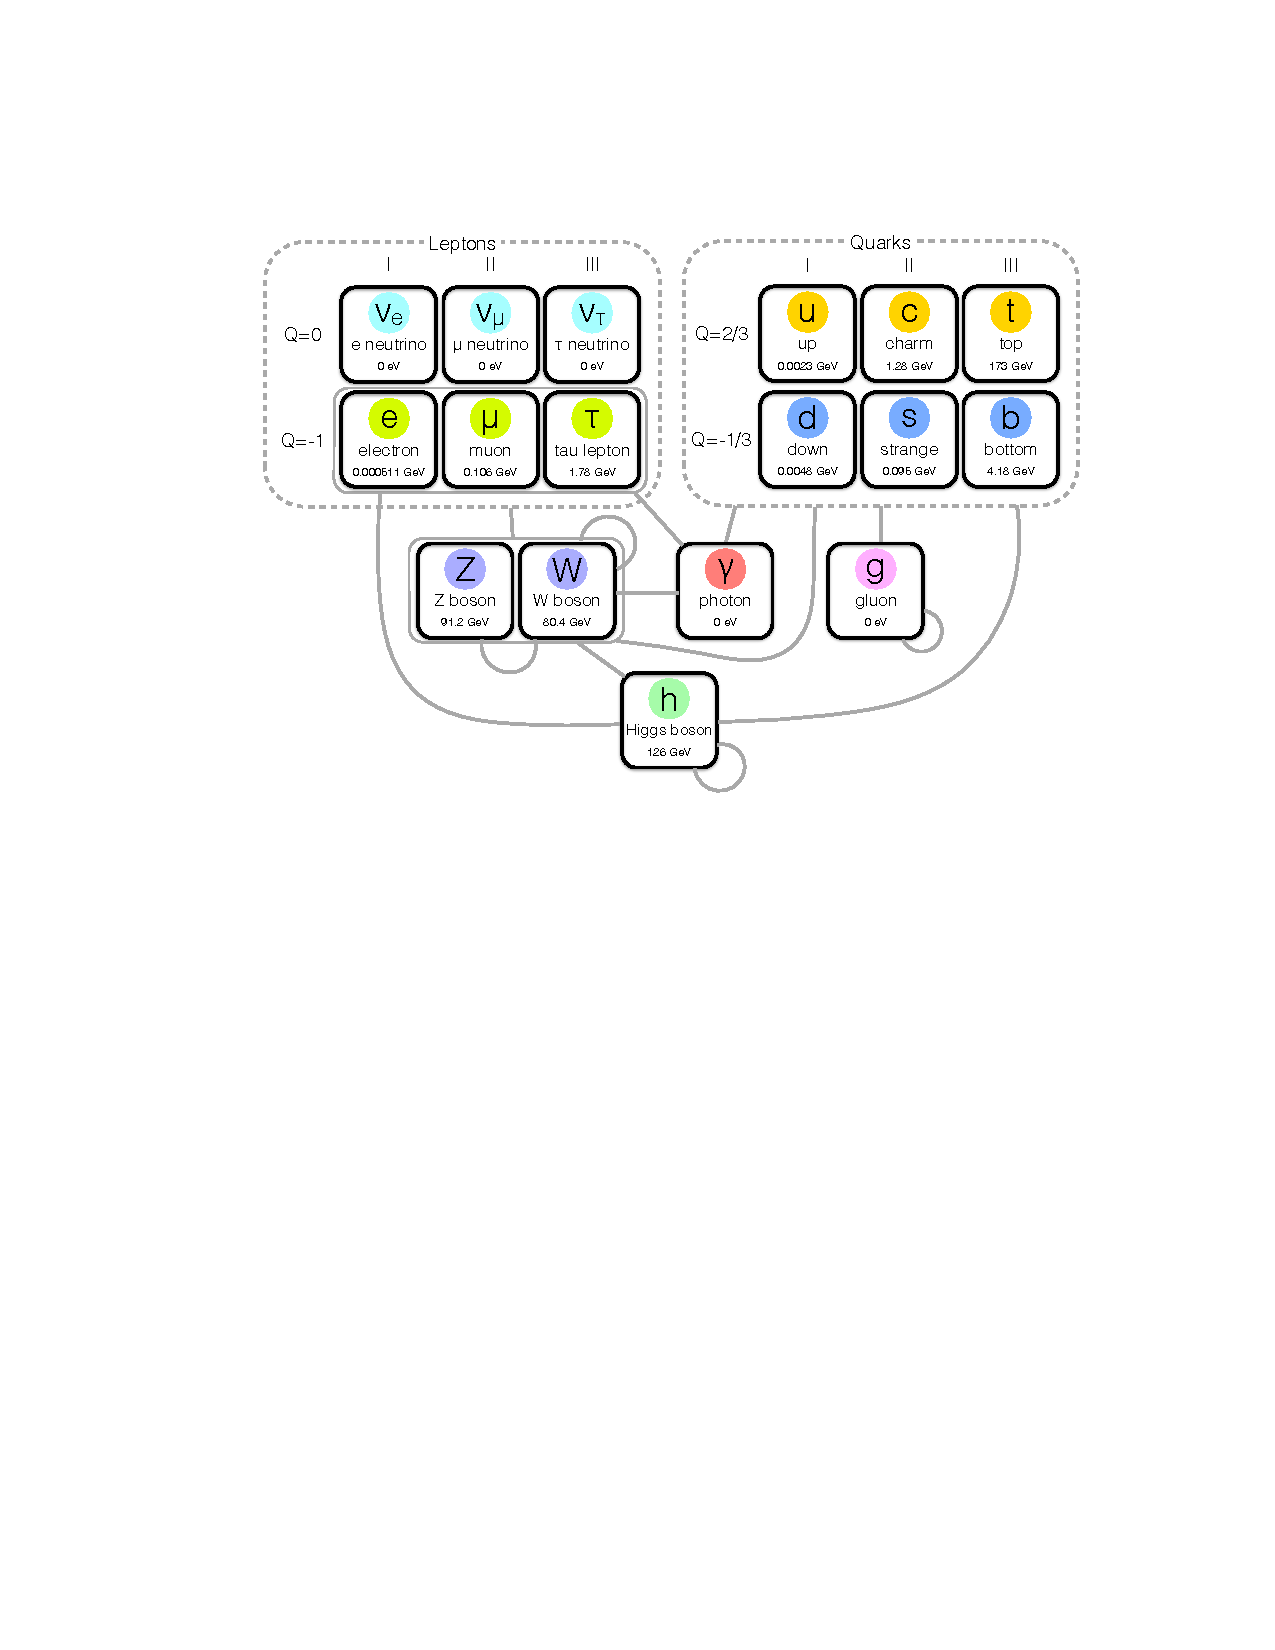
\includegraphics[width=\textwidth]{Figures/Theory/SM_Interactions.pdf}
    \caption{Particle content of the standard model. Allowed interactions are indicated with gray lines between particles or particle groups. The mass of each particle is listed underneath its symbol and name. The electric charge Q of the leptons and quarks is also indicated. Particles connected to themselves can have self-interactions.
    Reprinted from Reference~\cite{Yutaro}.}
    \label{fig:SMint}
\end{figure*}

%%%%%%%%%%%%%%%%%%%%%%%%%%%%%%%%%%%%%%%
%%%%%%%%%%%%%%%%%%%%%%%%%%%%%%%%%%%%%%%

\subsection{Electroweak symmetry breaking}
\label{sec:EWSB}
Electroweak symmetry breaking is a crucial feature of the standard model. The electroweak symmetry is spontaneously broken through the Higgs mechanism. 
The scalar potential of the complex Higgs field $H$ is
\begin{equation}
V(H^\dagger H) =  \mu^2(H^\dagger H) + \lambda(H^\dagger H)^2. 
\label{equ:HiggsV}
\end{equation}

The mass parameter $\mu^2$ is negative, which means that the vacuum expectation value (vev) of the Higgs (written as $\langle H \rangle$ or $v$) is non-zero. The Higgs potential is illustrated in Figure~\ref{fig:HiggsV}. Spontaneous symmetry breaking occurs when the value of the Higgs field ``rolls" from the unstable position at the origin and comes to rest at the stable minima:
\begin{equation}
\langle H \rangle= v = \sqrt{\frac{-\mu^2}{2\lambda}}.
\end{equation}
The value of $v$ has been measured in electroweak interactions to be about 174 Gev. 

\begin{figure*}[htbp]
    \centering
    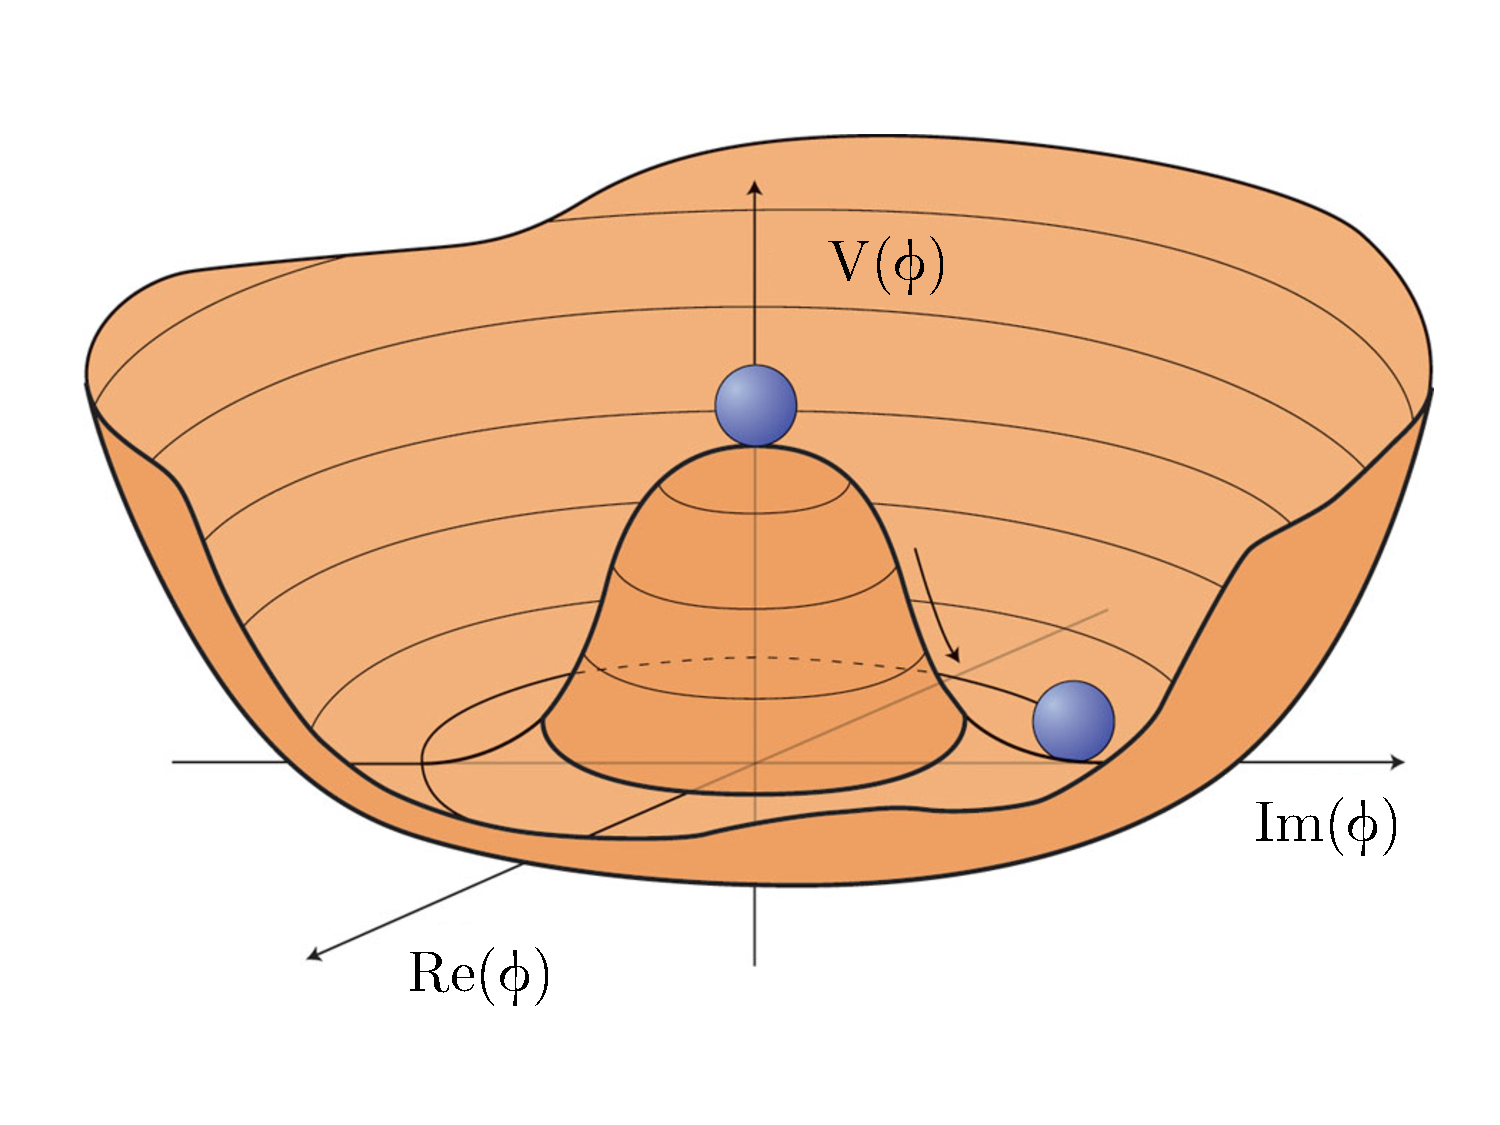
\includegraphics[width=0.8\textwidth]{Figures/Theory/improvedMexicanHat.pdf}
    \caption{Cartoon illustrating the Higgs potential. The Higgs field during spontaneous symmetry breaking can be thought of as the ball, which ``rolls" from the unstable point to the stable minima.
    Reprinted from Reference~\cite{mexicanHat}.}
    \label{fig:HiggsV}
\end{figure*}

During EWSB, three of the four degrees of freedom in the Higgs complex scalar doublet get ``eaten" to give mass to the $W^\pm$ and $Z$ bosons. The last degree of freedom becomes the 125 GeV scalar Higgs boson. The mass $m_H$ of the Higgs boson can be written in terms of the parameters $\mu$ and $\lambda$: 
\begin{equation}
m_H = \sqrt{-\mu^2} = v\sqrt{2\lambda}.
\label{equ:HiggsMass}
\end{equation}

The remaining symmetry is $U(1)_{\textrm{EM}}$, which corresponds to the electromagnetic interaction. The massless photon is the gauge boson of $U(1)_{\textrm{EM}}$ and couples to the electric charge Q: 
\begin{equation}
Q = T^3 + \Upsilon
\end{equation}
where $\Upsilon$ is the weak hypercharge and $T^3$ is the isospin. The short-range weak interactions are mediated by the $W^\pm$ and $Z$ bosons, and the photon mediates the long-range electromagnetic interactions.

%%%%%%%%%%%%%%%%%%%%%%%%%%%%%%%%%%%%%%%
\subsection{Limitations of the standard model}
\label{sec:SMweakness}
It is undeniable that the standard model has been a huge triumph of modern physics. However, there are known limitations. These fall into two categories: 
\begin{enumerate}
	\item Experimentally-established phenomena which are not incorporated into the standard model
	\item Unsettling questions that the standard model cannot answer but which perhaps would be explained by some more fundamental theory
\end{enumerate}

Neutrino masses---an example of the first category---have already been mentioned. The prevalence of matter over antimatter is another observed contradiction to the standard model as it exists today. The only SM source of CP violation is quark mixing, which is not nearly large enough to explain why the universe is more than just a bath of radiation from the annihilation of particles and antiparticles. 

The existence of dark matter also falls into the first category. A wealth of evidence, including galaxy cluster velocity dispersions, gravitational lensing studies, and measurements of the Cosmic Microwave Background, indicates that approximately 25\% of the energy budget of the universe is contained in dark matter (see Reference~\cite{DarkMatterReview} for a review). We know that dark matter interacts gravitationally, and stringent limits have been placed on the strength of its other interactions. However, so far there is no conclusive evidence as to the nature of dark matter.

The second category includes questions about why the 19 free parameters in the standard model have the values that they do. For instance, it could be seen as disconcerting that the masses of the particles in Figure~\ref{fig:SMint} cover such a large range, from $m_e = 0.000511$ GeV to $m_t = 173$ GeV. The problem of ``fine-tuning" is often discussed in this context. A theory is said to be fine-tuned if several free parameters have to take on precise values and interact in a convenient way in order to explain the observed results. While nothing is inherently wrong with fine-tuning, it as an unsatisfying way to solve a problem. Many people use fine-tuned parameters as sign-posts pointing to the existence of a broader theory in which the coincidences are explained.

The hierarchy problem\footnote{Much of the description here and in Section~\ref{sec:SUSY} is derived from the excellent pedagogical paper ``A Supersymmetry Primer" by Stephen P. Martin \cite{SUSYprimer}.} is a particularly worrisome fine-tuning problem. The squared mass parameter $\mu^2$ in the Higgs potential receives huge quantum corrections from loop diagrams. As already stated in Equation~\ref{equ:HiggsMass}, $\mu^2$ can be written in terms $v$ and $\lambda$, and $v$ has been measured to be approximately 174 GeV. Some fantastic cancellation must occur to counteract these quantum corrections, but there is no motivation for such cancellations in the standard model. 

Every particle that couples directly or indirectly to the Higgs field contributes to the quantum corrections to $\mu^2$. For a fermion $f$, the loop-level contributions come from the Feynman diagram of Figure~\ref{fig:hierarchy}a:
\begin{equation}
\Delta\mu^2 = -\frac{|\lambda_f|^2}{8\pi^2}\Lambda^2_\mathrm{UV} + ....
\label{equ:corrFermion}
\end{equation}
where the relevant term in the Lagrangian is $-\lambda_fH\bar{f}f$ and $\Lambda_\mathrm{UV}$ is the ultraviolet momentum cutoff of the theory \cite{SUSYprimer}. 

\begin{figure*}[htbp]
    \centering
    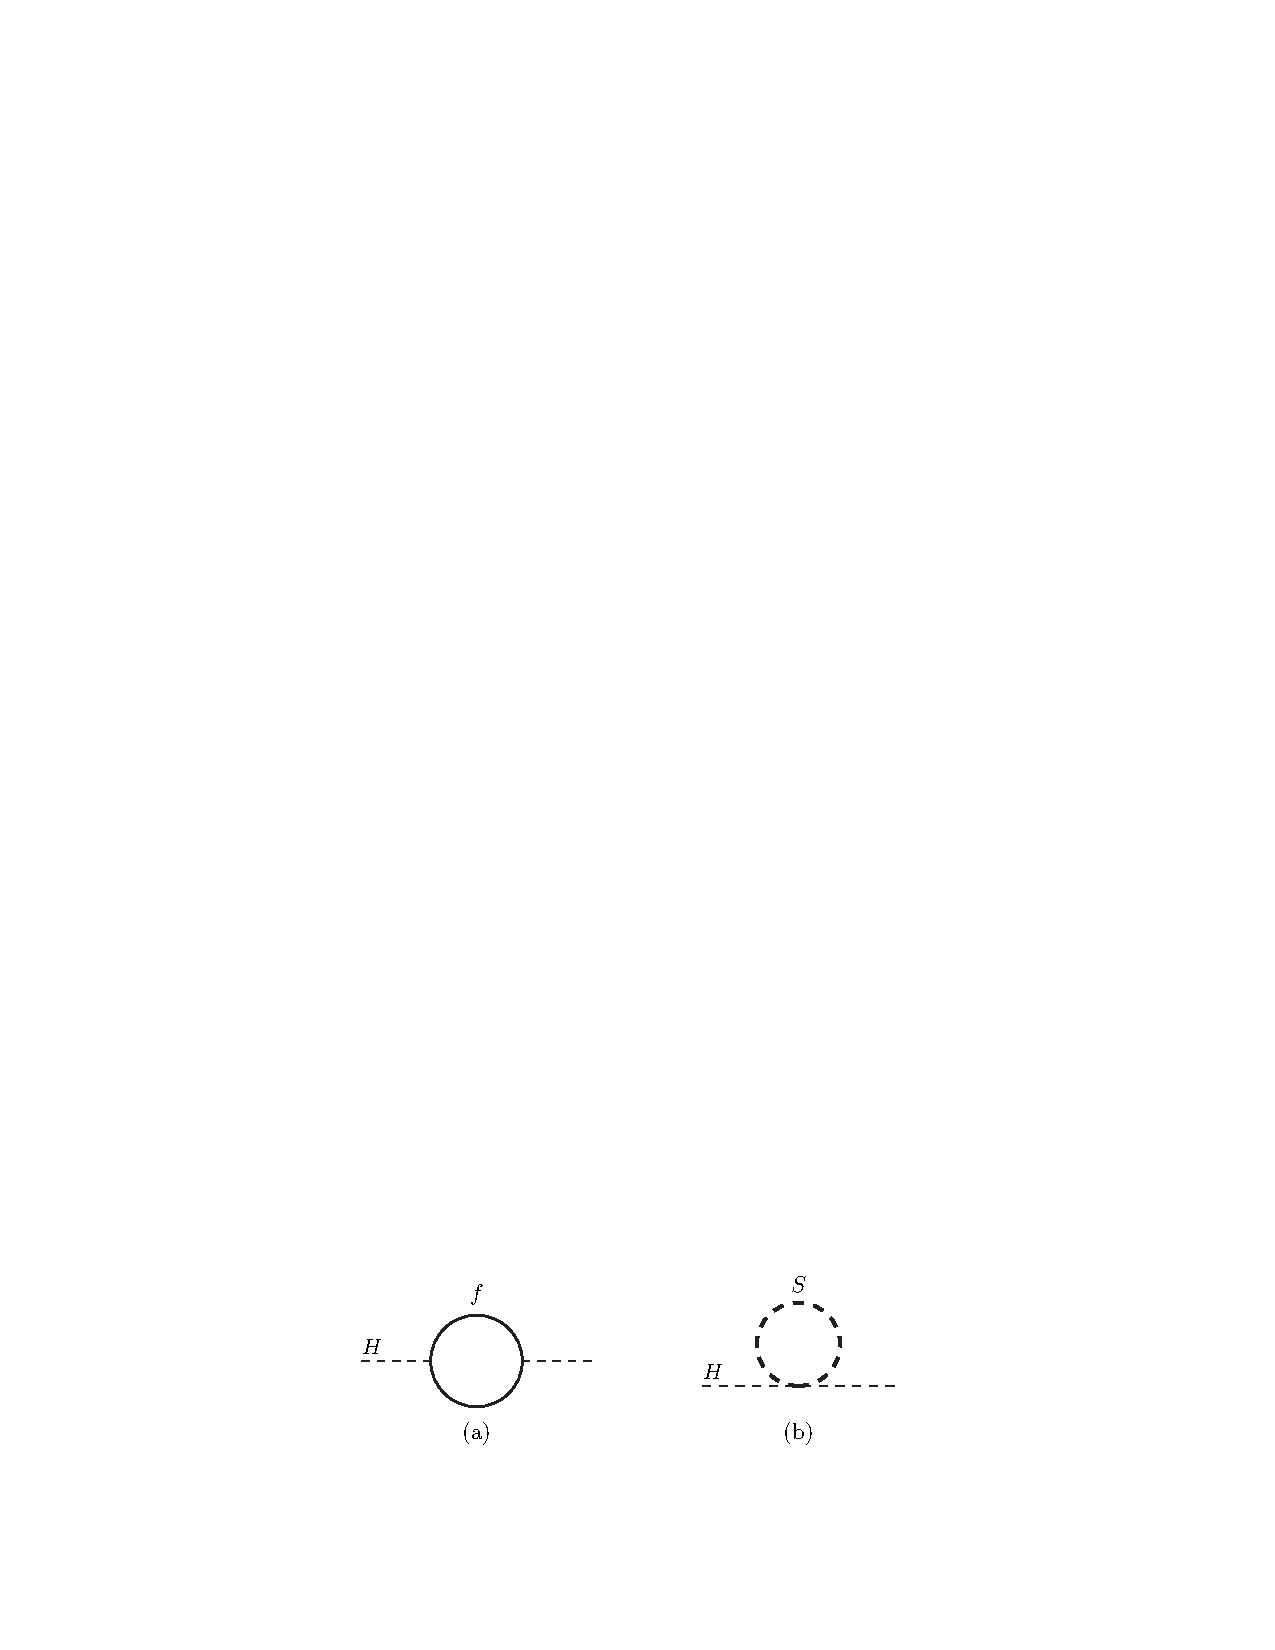
\includegraphics[width=0.7\textwidth]{Figures/Theory/hierarchyLoop.pdf}
    \caption{One-loop quantum corrections to the Higgs mass parameter $\mu^2$ from a Dirac fermion $f$ (left) and a scalar $S$ (right).
    Reprinted from Reference~\cite{SUSYprimer}.}
    \label{fig:hierarchy}
\end{figure*}


Even if it does not couple directly to the Higgs, any new particle would also contribute to $\mu^2$ at the two-loop level if it participates in the SM gauge interactions. For example, consider a heavy fermion $F$ with mass $m_F$ that only couples indirectly to the Higgs. Example two-loop Feynman diagrams are shown in 
\ref{fig:hierarchyFermi}. For such a fermion, the quantum corrections will be given by
\begin{equation}
\Delta\mu^2 = C(\frac{g^2}{16\pi^2})^2 [a \Lambda^2_\mathrm{UV} + 24m_F^2 \ln(\Lambda_\mathrm{UV}/m_F) +...]
\label{equ:corrTwoLoopFermi}
\end{equation}
where the constant $C$ represents several group theory factors, $a$ depends on the renormalization method, and $g$ is the gauge coupling. 

\begin{figure*}[htbp]
    \centering
    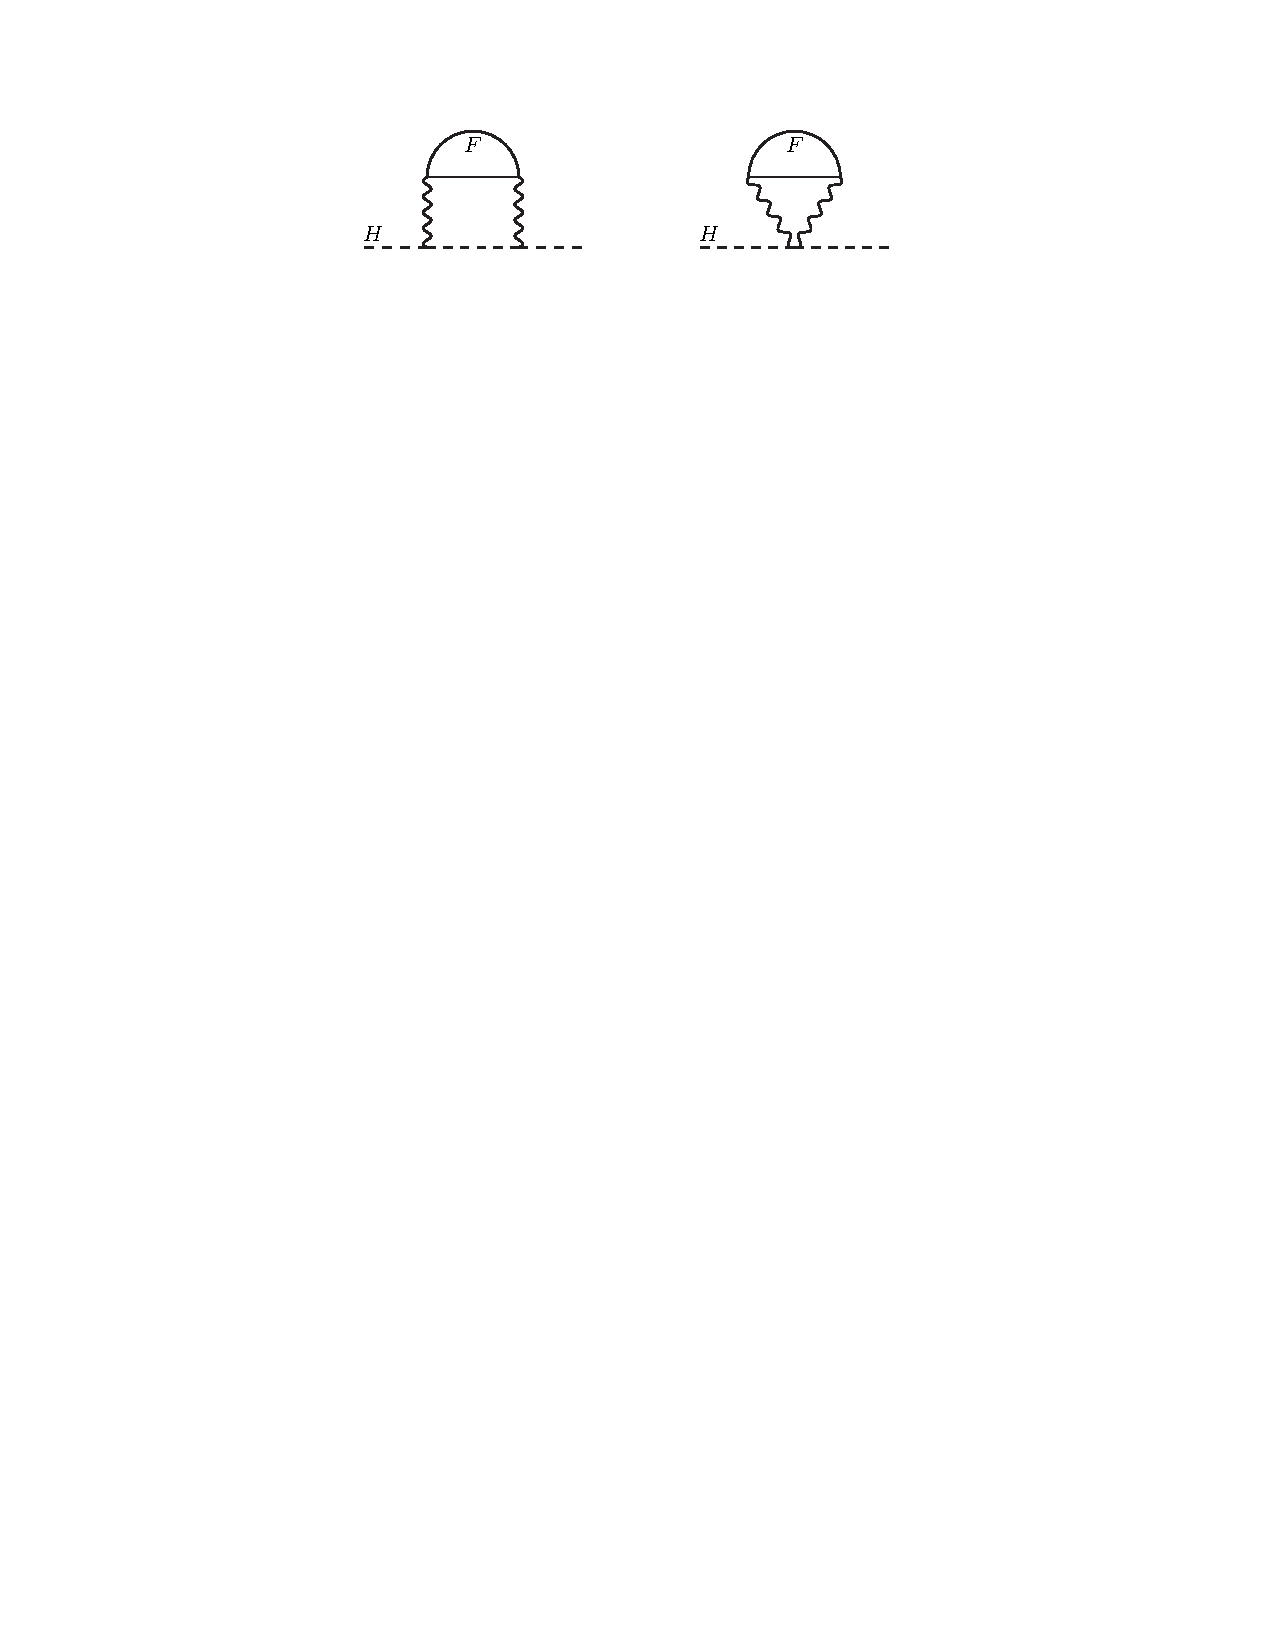
\includegraphics[width=0.7\textwidth]{Figures/Theory/hierarchyLoopFermi.pdf}
    \caption{Two-loop quantum corrections to the Higgs mass parameter $\mu^2$ from a fermion $F$ that couples indirectly to the Higgs through gauge interactions.
    Reprinted from Reference~\cite{SUSYprimer}.}
    \label{fig:hierarchyFermi}
\end{figure*}

The root of the hierarchy problem is the presence of $\Lambda^2_\mathrm{UV}$ in both Equations~\ref{equ:corrFermion} and \ref{equ:corrTwoLoopFermi}. If $\Lambda^2_\mathrm{UV}$ is near the Planck scale ($M_P = 2 \times 10^{18}$ GeV), then the corrections to $\mu^2$ are an unbelievable 30 orders of magnitude above its observed value. If we use dimensional regularization, it is possible to get rid of the $\Lambda^2_\mathrm{UV}$ terms in Equations~\ref{equ:corrFermion} and \ref{equ:corrTwoLoopFermi}, but the term proportional to $m_F^2$ remains \cite{SUSYprimer}. Since it seems incredibly unlikely that there are no new particles to be found in the 16 orders of magnitude between the electroweak and Planck scales, there is a tension between the experimentally-preferred and the theoretically-preferred values.

As will be discussed next, this observation has motivated many proposed extensions to the standard model, including supersymmetry.

%%%%%%%%%%%%%%%%%%%%%%%%%%%%%%%%%%%%%%%

%12 vector fields (spin 1)- gauge fields of the SU(3) x SU(2) x U(1)
%45 Weyl fermion fields: [21 Dirac spinors  (3 colors x 6 quarks) + 3 charged leptons] x2 to get to  weyl+ 3 neutrinos
%complex doublet H of scalar fields

%Left-handed Weyl components of quark Dirac spinors form 9 doublets of $SU(2)_W$ (3 flavor doublets per 3 color)
%Right-handed Weyl components of quark Dirac spinors are 18 $SU(2)_W$ singlets. Weak interactions can break parity

%Left-handed leptons form 3 $SU(2)_W$ doublets 
%right-handed leptons form singlets. If right-handed neutrinos exist, they are sterile and we have no evidence (can't have evidence?) for them
%Dirac spinor $\Psi$ and conjugate $\bar{\Psi}$ are equivalent to two left-handed Weyl spinors ($\chi$ and $\tilde{\chi}$)
%and their right-handed conjugates ($\chi^\dagger$ and $\tilde{\chi}^\dagger$).Tilde = anti


%http://bolvan.ph.utexas.edu/~vadim/Classes/2011f/SM.pdf

\section{Supersymmetry}
\label{sec:SUSY}

Supersymmetry (SUSY) is a particularly beautiful theoretical framework that addresses several of the standard model limitations described above. A ``supersymmetry" is a symmetry relating bosons and fermions. The supersymmetric operator $Q$ turns a bosonic state into a fermionic state:
\begin{equation}
Q|\mathrm{boson}\rangle = |\mathrm{fermion}\rangle, \hspace{35pt} Q|\mathrm{fermion}\rangle = |\mathrm{boson}\rangle
\label{equ:SUSYdef}
\end{equation}

The immediate consequence is that the number of elementary particles is at least double that in the standard model. For each SM boson, there will be a fermion ``superpartner" and vice versa. The deeper implications of Equation~\ref{equ:SUSYdef}, however, have many interesting effects, some of which 
provide attractive solutions to the issues with the SM listed above.

\subsection{Supersymmetric solution to the hierarchy problem}
\label{sec:SUSYhierarchy}

The key to solving the hierarchy problem with supersymmetry appears if we consider a heavy complex scalar $S$ with mass $m_S$. If the interaction term between $S$ and $H$ in the Lagrangian is $-\lambda_S|H|^2|S|^2$, then diagrams such as those in Figure~\ref{fig:hierarchy}b give rise to the following quantum corrections:
\begin{equation}
\Delta\mu^2 = -\frac{\lambda_S^2}{16\pi^2} [ \Lambda^2_\mathrm{UV} - 2 m_S^2 \ln{\Lambda_\mathrm{UV} / m_S) }+ ... ]
\label{equ:corrScalar}
\end{equation}

Upon close inspection of Equations~\ref{equ:corrFermion} and \ref{equ:corrScalar}, it becomes clear that if
there are two complex scalars per fermion that satisfy $\lambda_S = |\lambda_f|^2$, then the contributions to $\mu^2$ proportional to $ \Lambda^2_\mathrm{UV}$ cancel exactly. 
Less obvious is whether the contributions from diagrams with more loops also cancel. The good news is that it can be shown that 
the contributions to $\mu^2$ cancel to all orders in a supersymmetric theory. Any new particles, even extremely massive ones, would be
accompanied by their superpartners and $\mu^2$ would remain unaffected.

%%%%%%%%%%%%%%%%%%%%%%%%%%%%%%%%%%%%%%%
%%%%%%%%%%%%%%%%%%%%%%%%%%%%%%%%%%%%%%%
%%%%%%%%%%%%%%%%%%%%%%%%%%%%%%%%%%%%%%%

\subsection{Particles in minimal SUSY models}
\label{sec:SUSYparticles}
In a supersymmetric theory, the SM particles shown in Tables~\ref{tab:fermions} and \ref{tab:bosons} must be arranged into ``supermultiplets" containing the SM fermions and bosons and their superpartners. There must be an equal number of bosonic and fermionic degrees of freedom in each supermultiplet ($n_b$ and $n_f$, respectively). The SM particles fall into two types of supermultiplets:
\begin{itemize}
\item The standard model fermions belong to \textbf{chiral supermultiplets}. Each chiral supermultiplet contains one Weyl fermion ($n_f = 2$) and a complex scalar field ($n_b = 2$).
\item The spin-1 gauge bosons belong to \textbf{gauge supermultiplets}. Before EWSB, the gauge bosons are massless and have $n_b = 2$. Their superpartners are massless spin-1/2 Weyl fermions with $n_f = 2$. 
\end{itemize}

The Minimal Supersymmetric Standard Model (MSSM) is the most basic SM extension that incorporates SUSY. Table~\ref{tab:SUSY_fermions} lists the chiral supermultiplets in the MSSM, and the gauge supermultiplets are listed in Table~\ref{tab:SUSY_bosons}. Note that all particles in a supermultiplet are in the same representation of $G_{SM}$. 

There must be two Higgs chiral supermultiplets in the MSSM to avoid gauge anomalies in the electroweak gauge symmetry, one with hypercharge $\Upsilon = 1/2$ and one with $\Upsilon = -1/2$. The $\Upsilon = 1/2$ chiral supermultiplet $H_u$ has the Yukawa couplings necessary to give masses to the up-type quarks, and the Yukawa couplings of the $\Upsilon = -1/2$ chiral supermultiplet $H_d$ give masses to the down-type quarks. The 125 GeV standard model Higgs boson is a linear combination of $H_u^0$ and $H_d^0$.

%popular proposed SM extensions to solve the hierarchy problem. 
%%%%%%%%%%%%%%%%%%%%%%%%%%%%%%%%%%%%%%%

\begin{table}[ht]
    \caption{CHIRAL SUPERMULTIPLETS IN MSSM}
    \centering
    \begin{tabular}{|c|c|c|c|c|}
    \hline
    \hline
    \multicolumn{2}{|c|}{Names} & Spin 0 & Spin 1/2 &$SU(3)_C,~SU(2)_L,~U(1)_\Upsilon $\\
  	  \hline
           \hline    
squarks, quarks  & Q & ($\tilde{u}_L~\tilde{d}_L$) & ($u_L~d_L$)  & (\textbf{3}, \textbf{2}, $\frac{1}{6}$) \\
(3 families) & $\bar{u}$ & $\tilde{u}_R^\ast$ & $u_R^\dagger$ & ($\bar{\textbf{3}}$, \textbf{1}, $-\frac{2}{3}$) \\
                   & $\bar{d}$ & $\tilde{d}_R^*$     & $d_R^\dagger$ & ($\bar{\textbf{3}}$, \textbf{1}, $\frac{1}{3}$) \\
                   \hline
sleptons, leptons  & $L$ & ($\tilde{\nu}~\tilde{e}_L$) & ($\nu~e_L$)      &  (\textbf{1}, \textbf{2}, $-\frac{1}{2}$) \\
(3 families) & $\bar{e}$ & $\tilde{e}_R^\ast$  & $e_R^\dagger$ &  (\textbf{1}, \textbf{1}, 1) \\
\hline
Higgs, higgsinos & $H_u$  & ($H_u^+ ~ H_u^0$) & ($\tilde{H}_u^+ ~ \tilde{H}_u^0$) & ($\textbf{1}$, \textbf{2}, $+\frac{1}{2}$) \\
                           & $H_d$  & ($H_d^0 ~ H_d^-$) & ($\tilde{H}_d^0 ~ \tilde{H}_d^-$) & ($\textbf{1}$, \textbf{2}, $-\frac{1}{2}$) \\
           \hline
           \hline
    \end{tabular}
    \label{tab:SUSY_fermions}
    \justify{List of chiral supermultiplets in the MSSM. Reprinted from Reference~\cite{SUSYprimer}.}
\end{table}
%%%%%%%%%%%%%%%%%%%%%%%%%%%%%%%%%%%%%%%

\begin{table}[ht]
    \caption{GAUGE SUPERMULTIPLETS IN THE MSSM}
    \centering
    \begin{tabular}{|c|c|c|c|c|}
    \hline
    \hline
    Names & Spin 1/2 & Spin 1 &$SU(3)_C,~SU(2)_L,~U(1)_\Upsilon $\\
  	  \hline
           \hline    
gluino, gluon & $\tilde{g}$ & $g$   & (\textbf{8}, \textbf{1}, 0) \\
\hline
wino, $W$ bosons & $\widetilde{W}^\pm,~\widetilde{W}^0$ & $W^\pm,~W^0$ & (\textbf{1}, \textbf{3}, 0) \\
\hline
bino, $B$ boson & $\widetilde{B}^0$ & $B^0$ & (\textbf{1}, \textbf{1}, 0) \\
           \hline
           \hline
    \end{tabular}
    \label{tab:SUSY_bosons}
    \justify{List of gauge supermultiplets in the MSSM. Reprinted from Reference~\cite{SUSYprimer}.}
\end{table}

The names of the MSSM superpartners are very creatively derived from their SM counterparts. For fermions, the SM names are prefixed with ``s" to get the superpartner name: electrons to selectrons, quarks to squarks, etc. For bosons, the suffix ``ino" is added: $W$ to wino, gauge boson to gaugino, etc. The symbols for supersymmetric particles are given simply by adding a tilde to the SM symbol. For example, $\tilde{e}$ is the symbol for the selectron.

After EWSB, the neutral higgsinos ($\widetilde{H}_u^0$ and $\widetilde{H}_d^0$) and the neutral electroweak gauginos ($\widetilde{W}_0$ and $\widetilde{B}_0$) form four mass eigenstates known as neutralinos $\widetilde{\chi}^0$. The charged higgsinos ($\widetilde{H}_u^+$ and $\widetilde{H}_d^-$) and charged winos ($\widetilde{W}^\pm$) form four mass eigenstates known as charginos $\widetilde{\chi}^\pm$. 


%%%%%%%%%%%%%%%%%%%%%%%%%%%%%%%%%%%%%%%
%%%%%%%%%%%%%%%%%%%%%%%%%%%%%%%%%%%%%%%

\subsection{$R$-parity}
\label{sec:Rparity}
Phenomenologically, an important feature of many SUSY models is $R$-parity conservation.
$R$-parity is a new symmetry introduced in the MSSM to get rid of interactions that violate lepton number $L$
or baryon number $B$. 
Experimentally, we know that if $B$- and $L$-violating processes occur, they must be extremely suppressed. 
In particular, the lifetime of the proton must be greater than $10^{32}$ years \cite{SUSYprimer}. 
Without $R$-parity conservation, however, it is possible to write down terms in the MSSM Lagrangian 
that would allow the proton to decay to $e^+\pi^0$ or other 
lepton + meson combinations with a lifetime of less than one second.

$R$-parity (also known as matter parity) is a conserved quantum number:
\begin{equation}
P_R = (-1)^{3(B-L)+2s}
\end{equation}
where $s$ is the spin of the particle. All terms in the Lagrangian are required to satisfy $\prod P_{R} = +1$, where the product
is over all fields in the term. The SM particles and the Higgs bosons have $P_R = +1$, and
all SUSY particles---squarks, sleptons, gauginos, and higgsinos---have $P_R = -1$.

Most models of SUSY, including those explored in this analysis, assume $R$-parity conservation.
One immediate consequence is that each vertex must have an even number of supersymmetric particles (``sparticles").
In a collider experiment 
%where there are no SUSY particles initially, 
this means that sparticles must be pair-produced.
Additionally, $R$-parity conservation implies that the lightest supersymmetric particle (LSP) must be absolutely stable.
All other sparticles will eventually decay to the LSP. From the high energy experimentalist's point of view, this means that the 
primary signature of SUSY production in colliders will be significant missing transverse momentum. 
From the cosmologist's point of view, this means that the LSP, if electrically neutral, 
is a potential dark matter candidate

%%%%%%%%%%%%%%%%%%%%%%%%%%%%%%%%%%%%%%%
%%%%%%%%%%%%%%%%%%%%%%%%%%%%%%%%%%%%%%%
%%%%%%%%%%%%%%%%%%%%%%%%%%%%%%%%%%%%%%%
%%%%%%%%%%%%%%%%%%%%%%%%%%%%%%%%%%%%%%%
%%%%%%%%%%%%%%%%%%%%%%%%%%%%%%%%%%%%%%%
%cite http://pdg.lbl.gov/2015/reviews/rpp2015-rev-susy-2-experiment.pdf

\section{Gauge-mediated supersymmetry breaking}
\label{sec:gmsb}

So far no SUSY particles have been observed. If SUSY were an unbroken symmetry, then the masses of the superpartners
would be the same as their SM counterparts. The lack of experimental detection means that SUSY must be a broken symmetry.
Theorists have come up with many different mechanisms by which SUSY can be broken. 
The SUSY breaking mechanism and the SUSY breaking scale 
determine the phenomenology of the model, including the SUSY particle masses and their allowed decay modes.

In gauge-mediated supersymmetry breaking (GMSB), SUSY is spontaneously broken in a ``hidden" sector that is decoupled from the SM interactions. 
New chiral supermultiplets known as messengers interact with the hidden sector and 
also interact with the ``visible" sector (ie, SM particles and their superpartners) through the normal
SM gauge interactions. The messengers are said to communicate between the two sectors and relay the information about the SUSY breaking.
From the lack of experimental observation, we know that the masses of the messenger particles must be very high. 

One of the nice features of GMSB is that the flavor symmetry of the SM is preserved, because the gauge interactions are flavor-blind. 
The messengers give mass to the sparticles through loop diagrams such as those shown in 
Figure~\ref{fig:GMSBgaugino} for gauginos and Figure~\ref{fig:GMSBscalars} for the squarks and sleptons. 

\begin{figure*}[htbp]
    \centering
    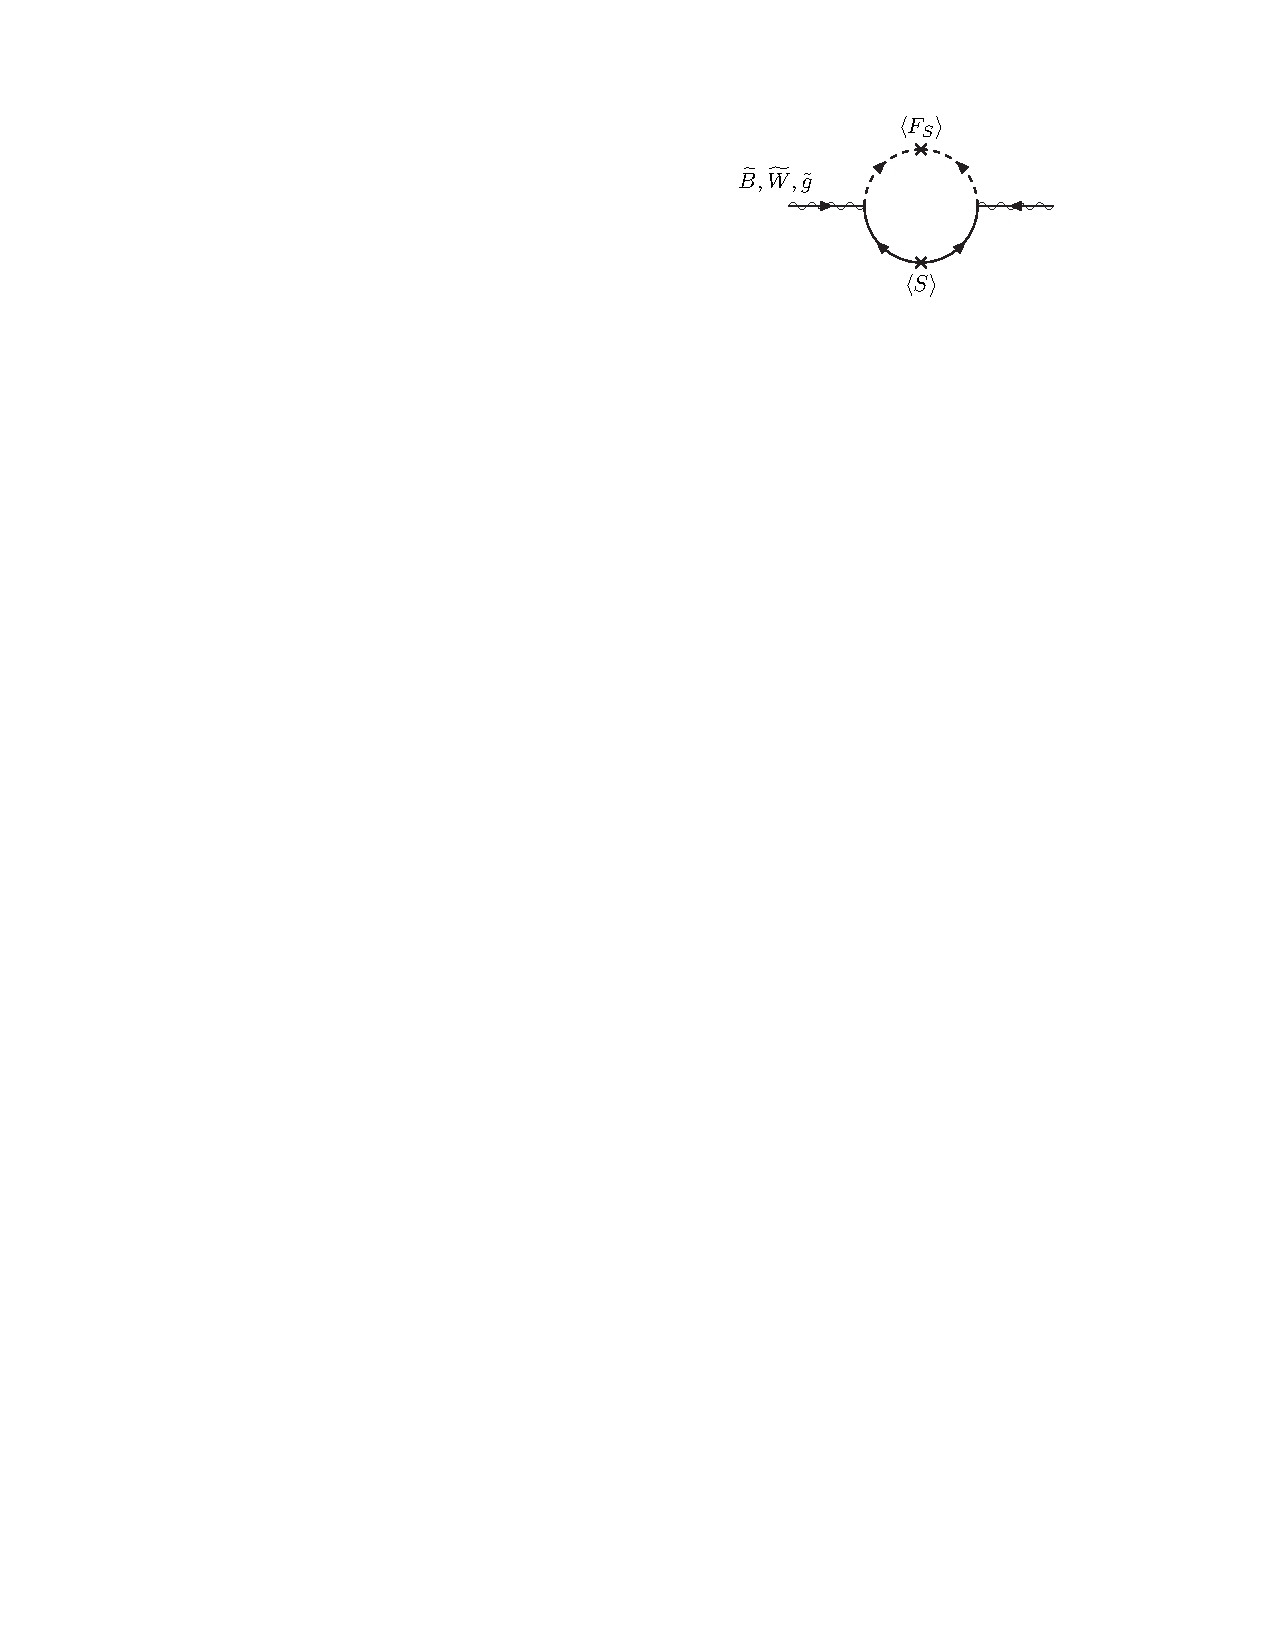
\includegraphics[width=0.4\textwidth]{Figures/Theory/GMSBgaugino.pdf}
    \caption{Feynman diagram illustrating how the messenger particles in SUSY models
    with general gauge mediation give rise to mass terms for the MSSM gauginos. 
    Wavy lines superimposed on straight lines represent the gauginos, and 
    $\langle F_S \rangle$ and $\langle S \rangle$ represent messenger particles.
    Reprinted from Reference~\cite{SUSYprimer}.}
    \label{fig:GMSBgaugino}
\end{figure*}

\begin{figure*}[htbp]
    \centering
        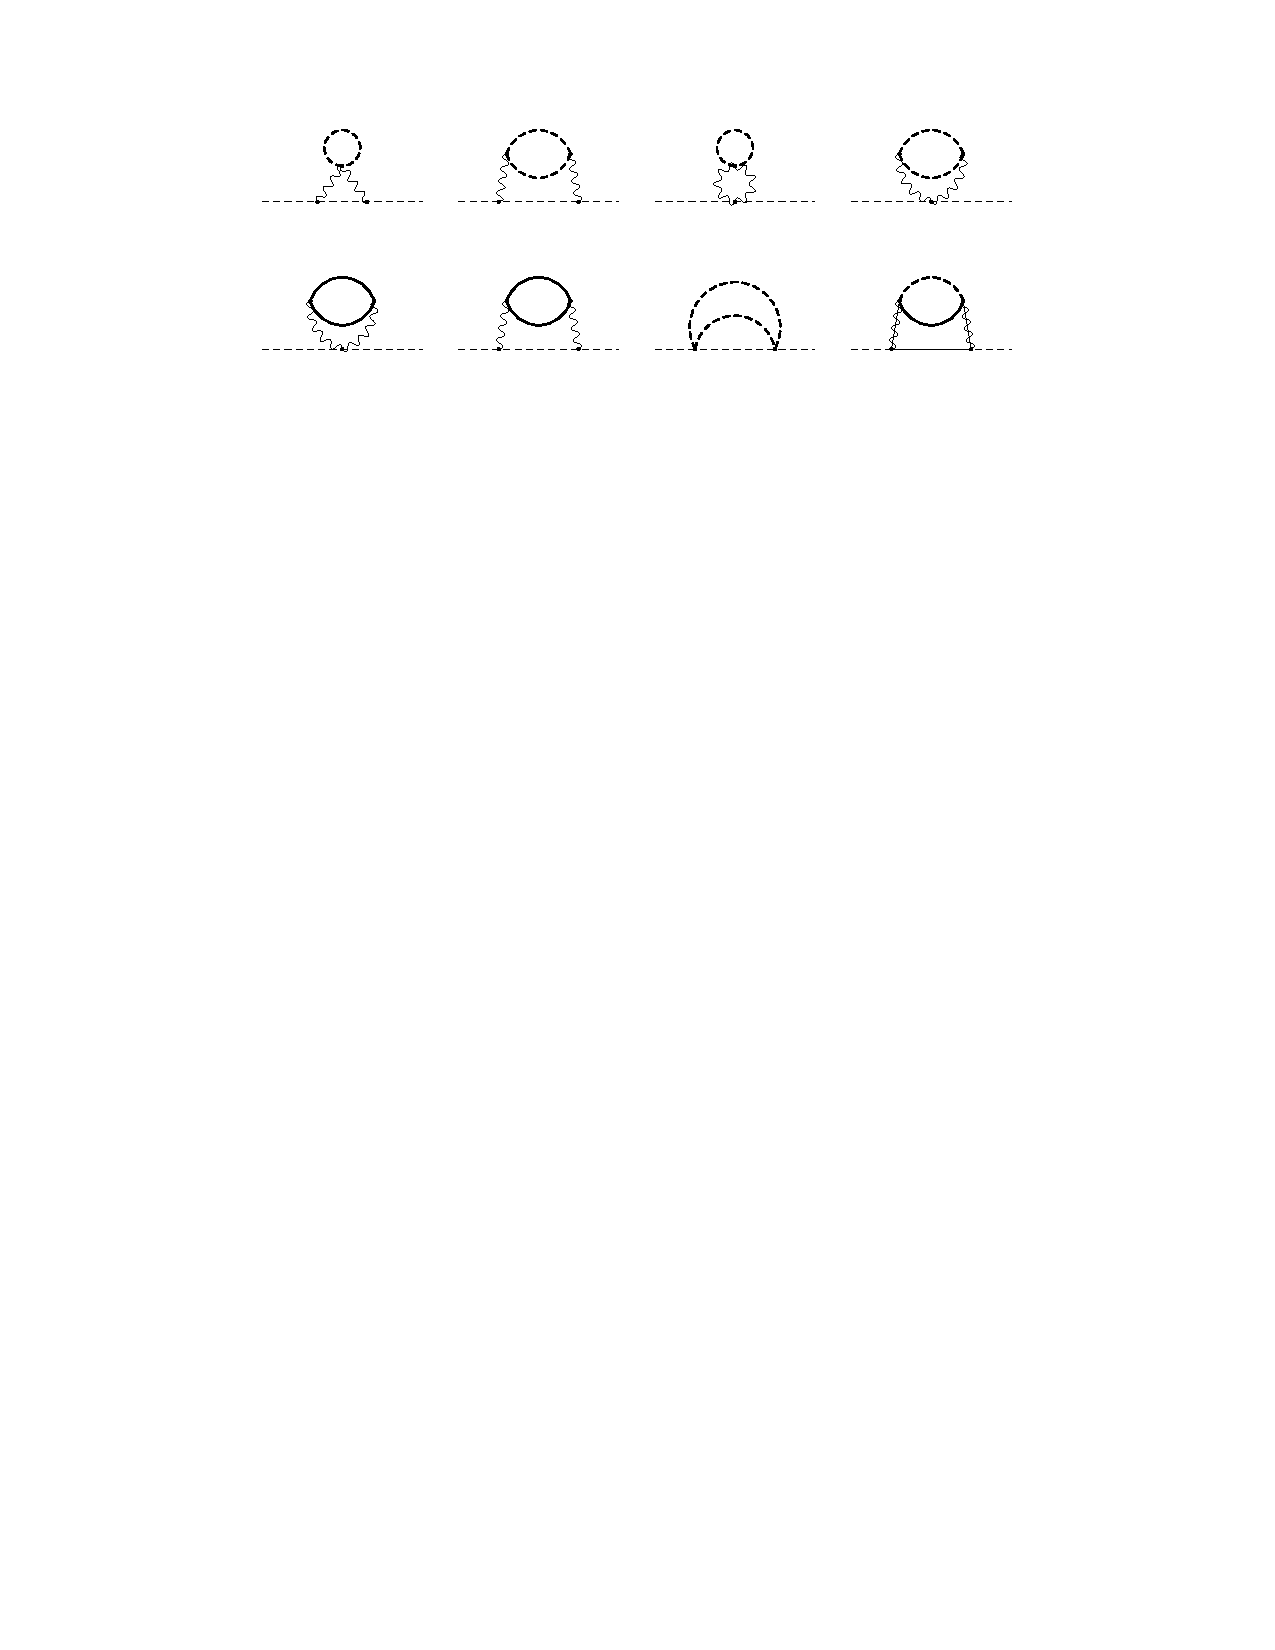
\includegraphics[width=\textwidth]{Figures/Theory/GMSBscalar.pdf}
    \caption{Example Feynman diagrams illustrating how the messenger particles in SUSY models
    with general gauge mediation give rise to mass terms for 
    the MSSM scalars. Wavy lines superimposed on straight lines represent the MSSM gauginos, 
    dotted lines represent the MSSM scalars, wavy lines represent the SM gauge bosons, heavy dashed lines
    represent messenger scalars, and solid lines represent messenger fermions.
    Reprinted from Reference~\cite{SUSYprimer}.}
    \label{fig:GMSBscalars}
\end{figure*}

GMSB usually refers to the minimal version of the theory, where the hidden sector includes a single field $S$ that is a singlet under $G_{SM}$. 
The more general framework is referred to as general gauge mediation (GGM). 

The GGM phenomenology is independent from the exact SUSY-breaking mechanism in the hidden sector. In particular, 
in all GGM models, the lightest supersymmetric particle is the gravitino \gravitino, the superpartner of the graviton. 
The graviton is a spin-2 particle, which means the graviton and gravitino can not belong to either the chiral or gauge supermultiplets described in Section~\ref{sec:SUSYparticles}. Instead, the gravitino is a spin-3/2 particle.

In GGM, the gravitino must be significantly lighter than all other sparticles, on the order of eV to keV. The gravitino only interacts
gravitationally with SM particles and therefore escapes the detector without depositing its energy. This causes 
an imbalance in the reconstructed momentum in the transverse plane of the detector and is referred to as missing 
transverse momentum $\vec{\pt}^{\mathrm{miss}}$. The magnitude of $\vec{\pt}^{\mathrm{miss}}$ is called the
missing transverse energy, or \ETmiss.

The next-to-lightest supersymmetric particle (NLSP) is either the lightest chargino or the lightest neutralino.
In this analysis, we will only consider models where the NLSP is the neutralino. We further constrain 
ourselves to models where the neutralino decays promptly. In general, the allowed neutralino decays are
$\neutralino \rightarrow \gamma\gravitino$, $\neutralino \rightarrow H\gravitino$, or $\neutralino \rightarrow Z\gravitino$,
but the first case normally dominates. We will assume 100\% branching fraction of $\neutralino \rightarrow \gamma\gravitino$
for the interpretation of our results.

If we assume $R$-parity conservation, then sparticles must be pair-produced and eventually decay to a gravitino. 
In a $p$-$p$ collider such as the LHC, the dominant production modes for SUSY particles are either gluino pair production
or squark pair production. Example decay chains are shown in Figure~\ref{fig:gluinoSquarkDecay1}. The final state 
signature is characterized by two photons and significant \ETmiss.

\begin{figure*}[htbp]
    \centering
    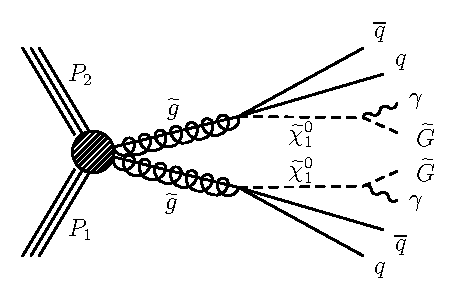
\includegraphics[width=0.45\textwidth]{Figures/Results/gluinoDecay.pdf}
    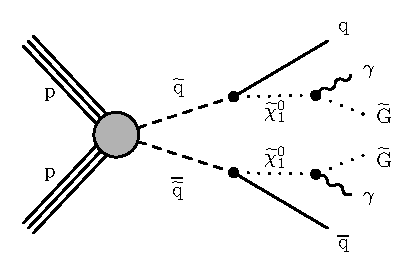
\includegraphics[width=0.45\textwidth]{Figures/Results/squarkDecay.pdf}
    \caption{Diagrams showing the production of signal events in the collision
        of two protons with four momenta ${P}_{1}$ and ${P}_{2}$. 
        The diagram on the left illustrates the decay chain for gluino pair production, and 
        the diagram on the right illustrates it for squark pair production. In both cases, 
        two neutralinos \neutralino are produced that each subsequently decay to a photon $\gamma$~and a gravitino \gravitino.
        In the diagram on the right, we do not distinguish between squarks and
        antisquarks.}
    \label{fig:gluinoSquarkDecay1}
\end{figure*}

\section{Experimental bounds on supersymmetry}
\label{sec:SUSYlimits}

So far, there has been no experimental evidence for supersymmetry. In the absence of evidence, limits
are placed on the allowed sparticle masses and SUSY process cross sections. 
During Run I of the LHC at CERN,
protons were collided at a center-of-mass energy $\sqrt{s} = 8$ TeV, setting a new record for high energy
collisions. No signs of physics beyond the standard model were observed. In 2015, the LHC successfully 
restarted at an even higher center-of-mass-energy, $\sqrt{s} = 13$ TeV. The increase in energy corresponded
to a large jump in discovery potential, but evidence for SUSY has still eluded us. 

Figure~\ref{fig:CMSexclusions} shows the excluded mass regions for EWK gauginos, squarks, and gluinos
from a wide variety of $\sqrt{s} = 13$ TeV CMS analyses \cite{SUSYtwiki}. Gluino masses below approximately 1800 GeV and 
squark masses below approximately 1000 GeV have been excluded at the 95\% confidence level. 
Figure~\ref{fig:CMSexclusions} does not contain any results interpreted in the context of GGM models.
The difference between the orange and blue bars illustrate the effect of nearly tripling the size of the
data set, from 12.9 \fbinv to 35.9 \fbinv. See Reference~\cite{pdgReview} for an full overview of SUSY 
limits from both colliders and precision measurements.

\begin{figure*}[htbp]
    \centering
    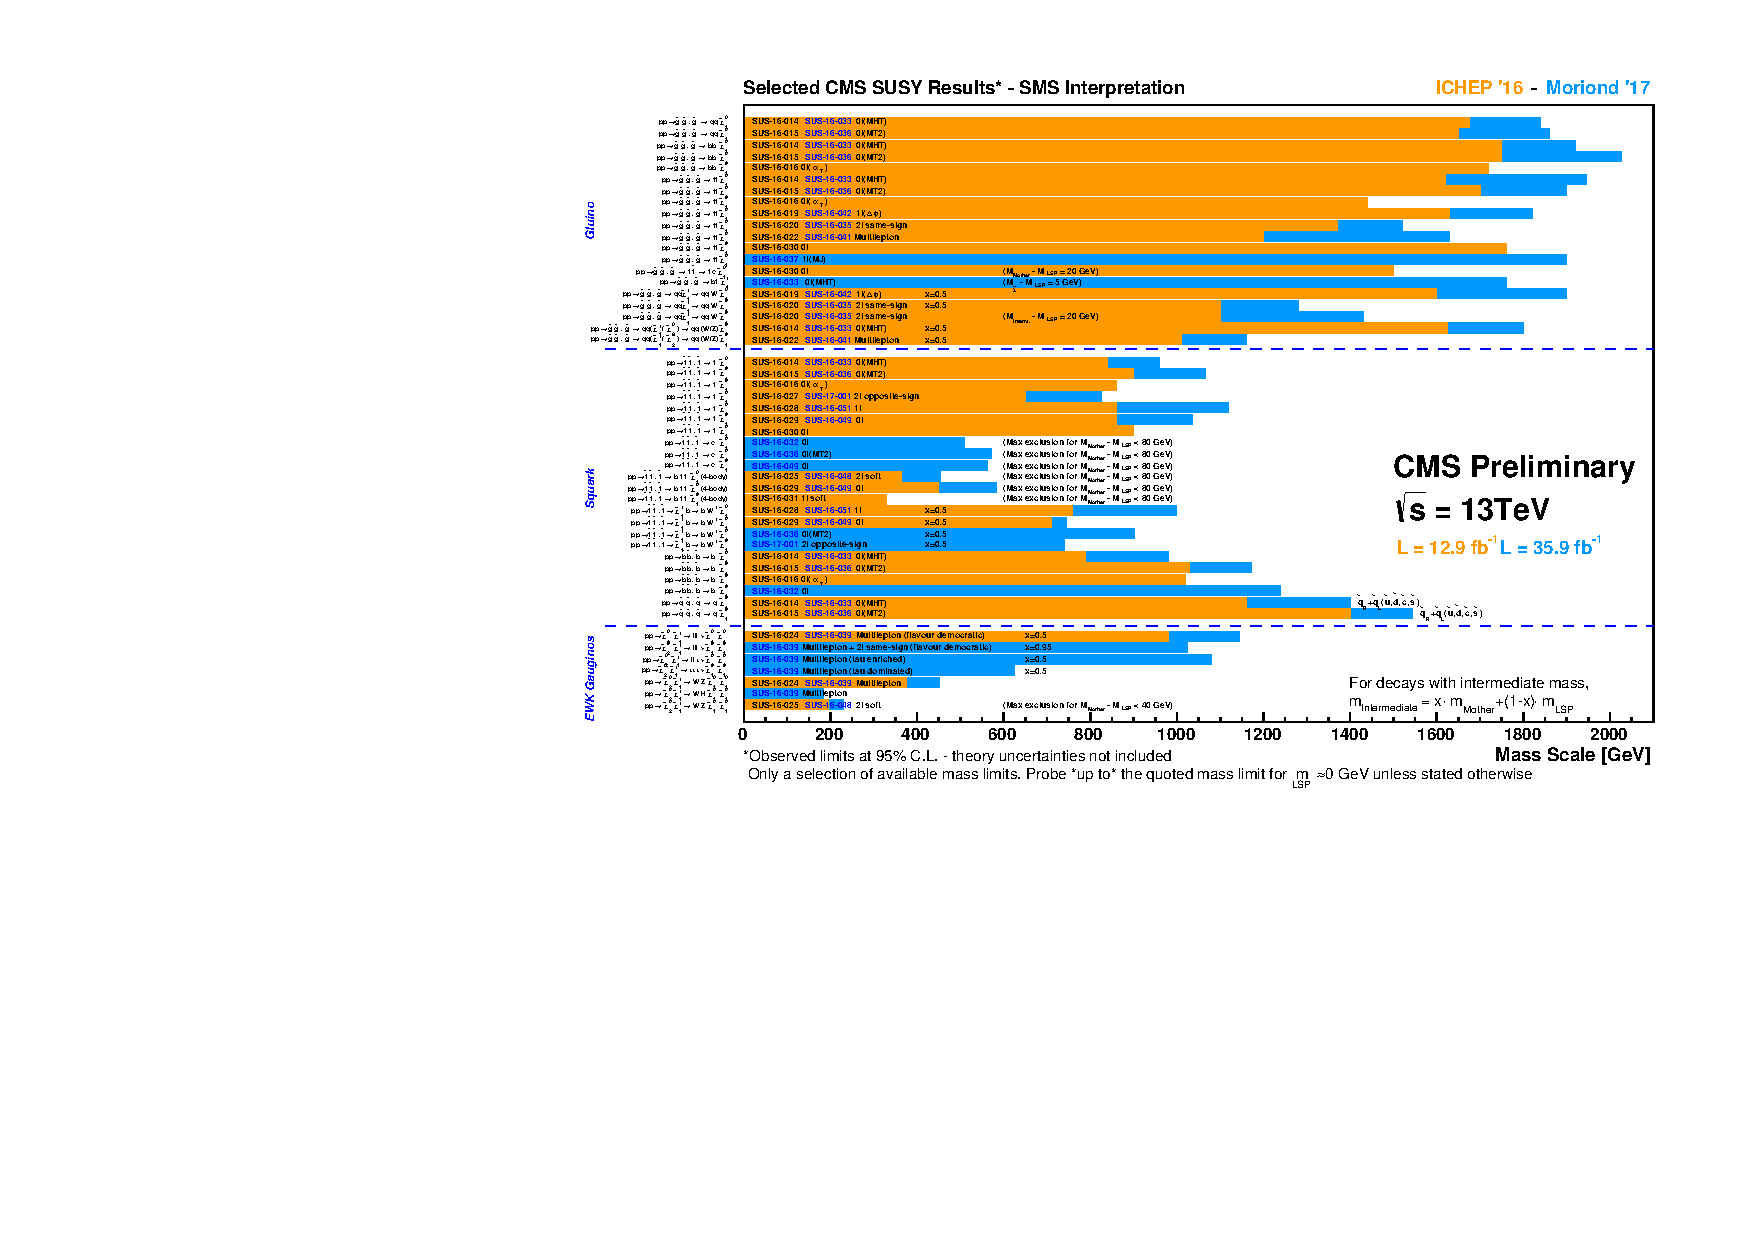
\includegraphics[angle=90,origin=c,width=.9\textwidth]{Figures/Theory/Moriond2017_BarPlot.pdf}
    \caption{ Excluded sparticle mass ranges for a selection of CMS results using the 2016 data set \cite{SUSYtwiki}.}
    \label{fig:CMSexclusions}
\end{figure*}

\subsection{Exclusion contours for GGM in the diphoton final state}
\label{sec:GMSBlimits}
Both CMS and ATLAS have published searches for GGM models in the diphoton final state, both at 8 TeV \cite{Aad:2015hea,Khachatryan:2015exa} and at 13 TeV \cite{ATLAS:2016aa,CMS:2015_anal}. Figure~\ref{fig:Limits2015CMS} shows the 95\% confidence level limits in the gluino versus neutralino and the squark versus neutralino mass planes using 2.3 \fbinv of 13 TeV data collected with the CMS detector in 2015. 
Gluino masses below 1.65 TeV and squark masses below 1.37 TeV have been excluded.
The simplified models used for the interpretation of results in Figure~\ref{fig:Limits2015CMS} will be described in more detail in Section~\ref{sec:SimplifiedModels}.

\begin{figure*}[h]
\begin{center}
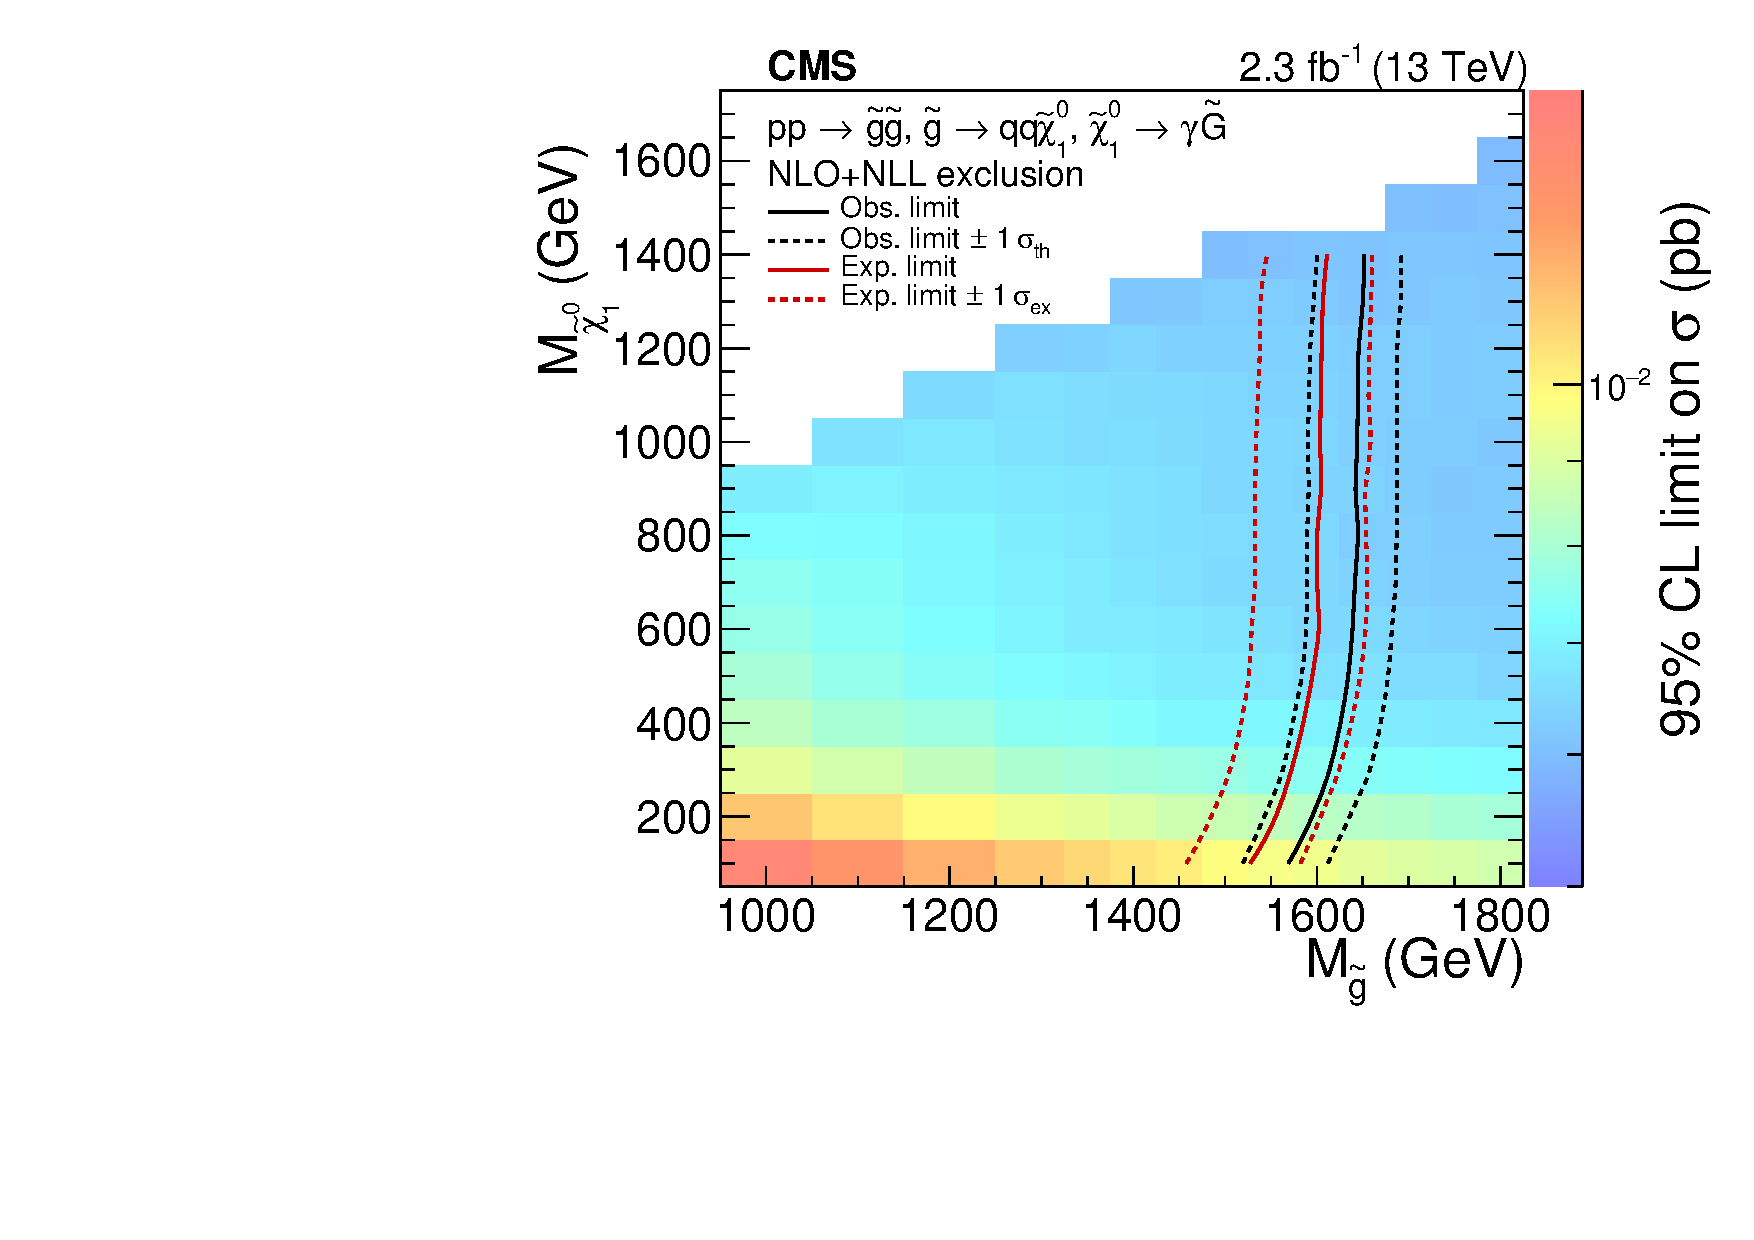
\includegraphics[width=0.49\textwidth]{Figures/Theory/2015gg.pdf}
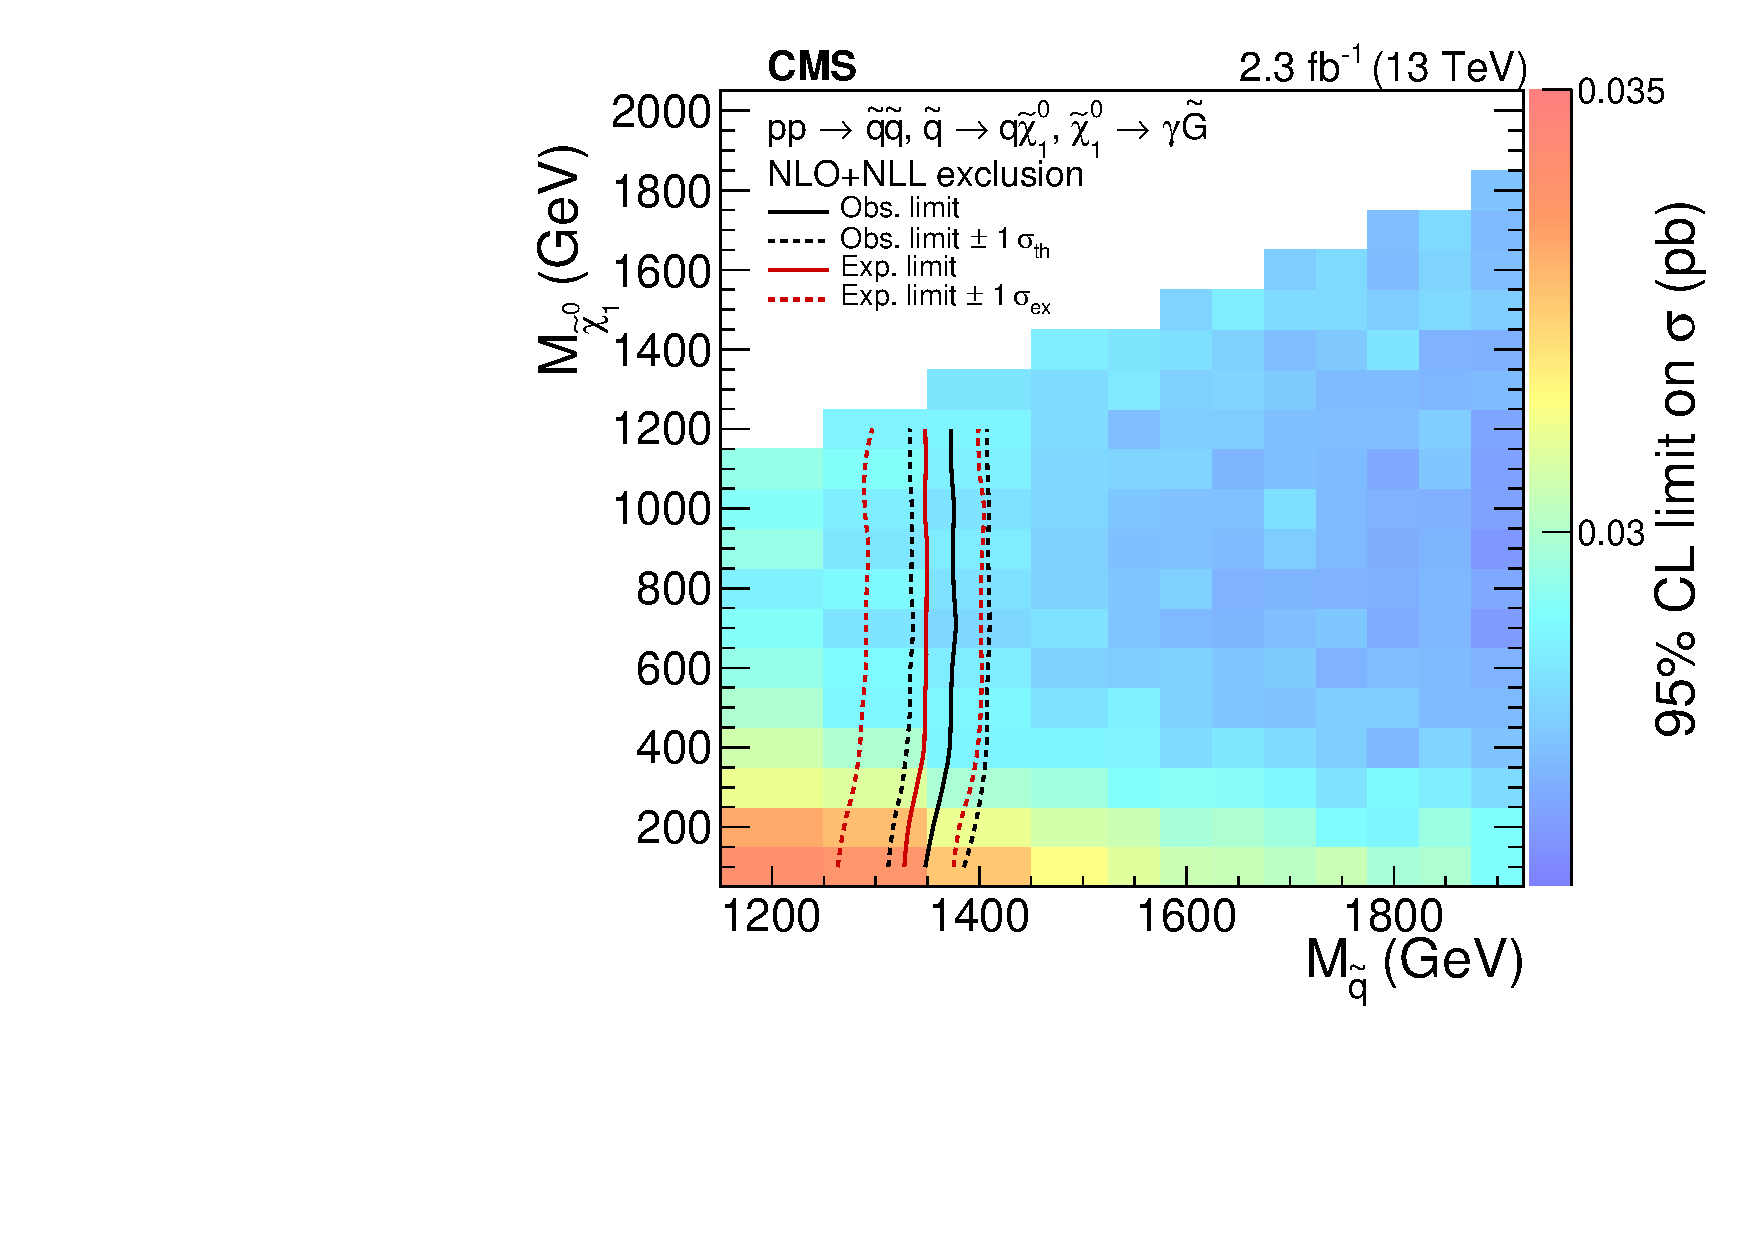
\includegraphics[width=0.49\textwidth]{Figures/Theory/2015qq.pdf}
\end{center}
    \caption{The 95\% CL upper limits on the gluino (left) and squark (right)
        pair production cross sections as a function of neutralino versus
	gluino or squark mass. The contours show the observed and median
        expected exclusions with their one
        standard deviation uncertainties. Reprinted from \cite{CMS:2015_anal}.}
    \label{fig:Limits2015CMS}
\end{figure*}

The 2015 ATLAS results are shown in Figure~\ref{fig:Limits2015ATLAS}. 
Limits were placed only on the masses of particles in a gluino pair production model. 
Gluino masses below 1.65 TeV were excluded at a 95\% confidence level.
The search strategy of the ATLAS analysis is similar to the CMS strategy. 
The primary difference is that ATLAS defines their signal regions so that the expected SM background is close to zero. 
This is the source of the asymmetric expected limits in Figure~\ref{fig:Limits2015ATLAS}.
The CMS methodology as applied to the 2016 data set is the main focus of this dissertation and 
will be described in detail, particularly in Chapter~\ref{chap:DataAnalysis}. 


\begin{figure*}[h]
\begin{center}
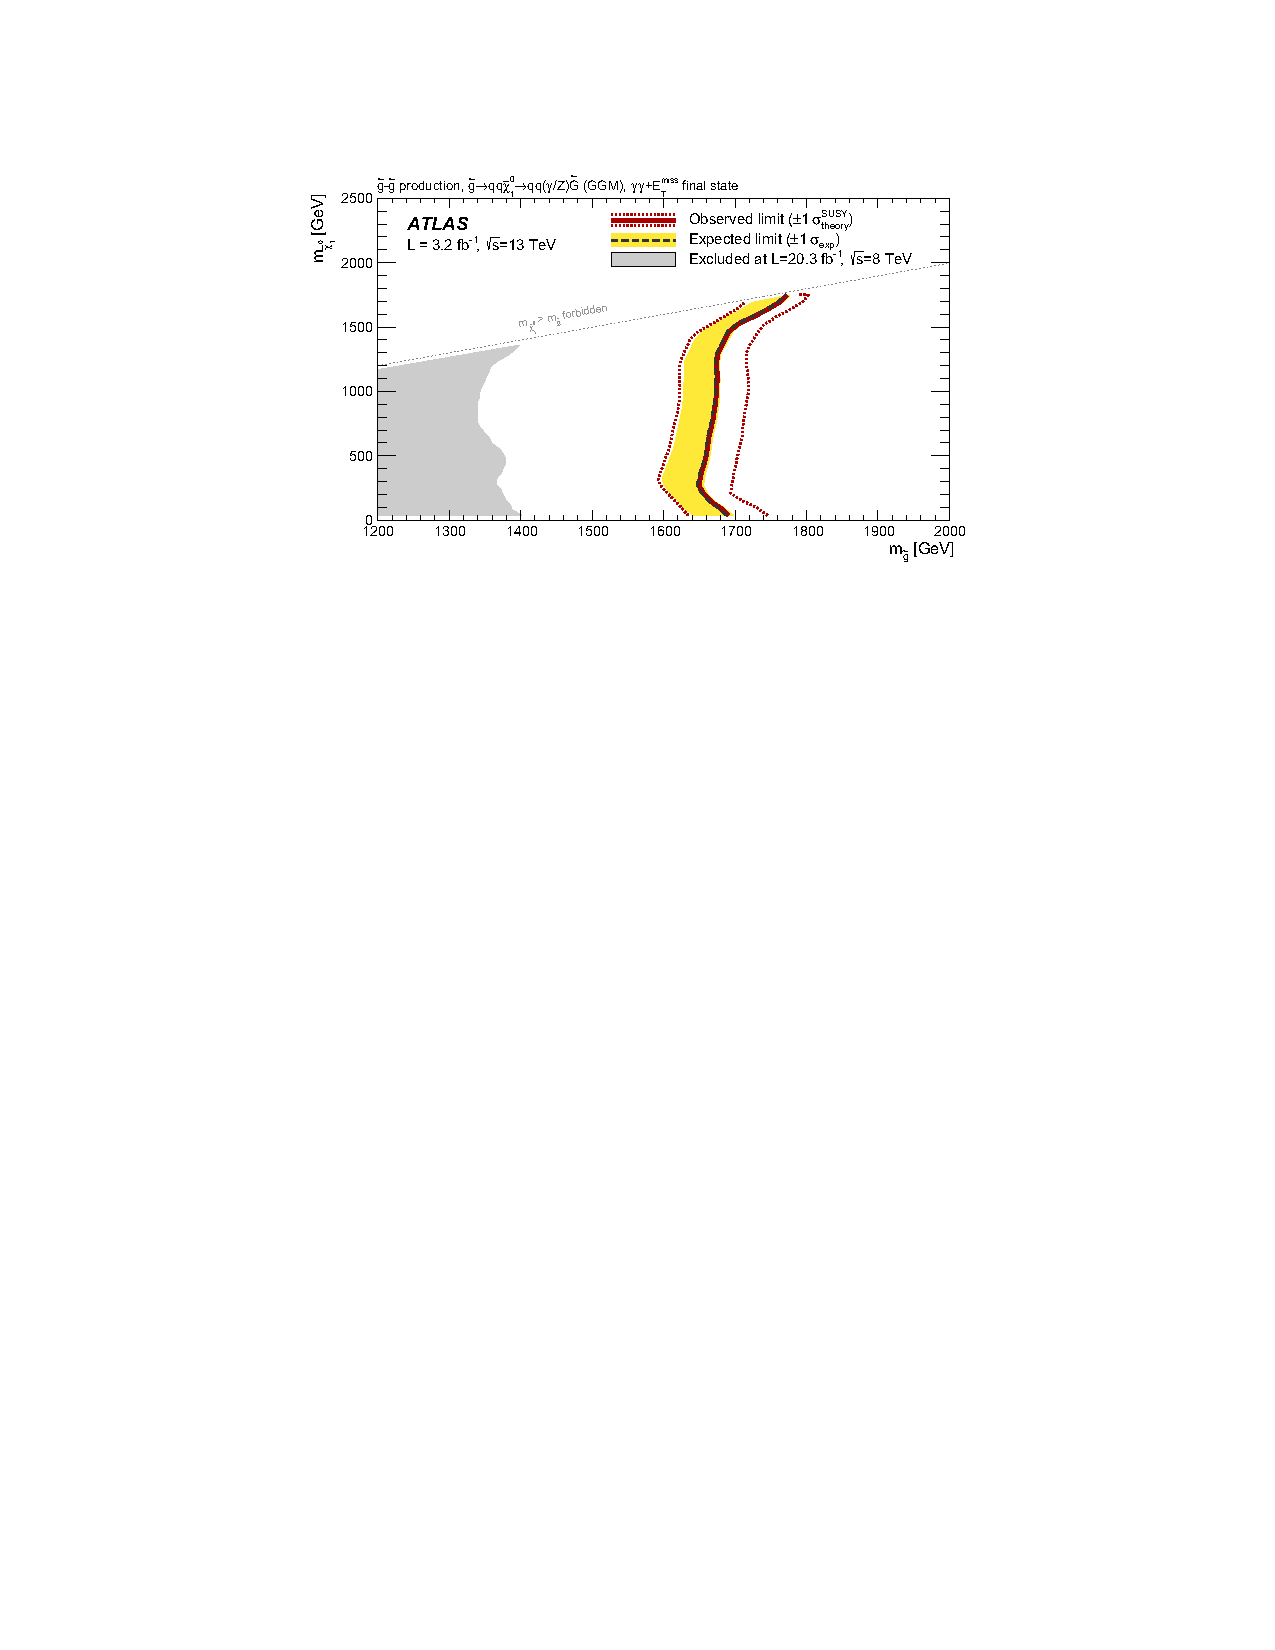
\includegraphics[width=0.8\textwidth]{Figures/Theory/2015ATLAS.pdf}
\end{center}
    \caption{95\% confidence level exclusion contours in the neutralino-gluino mass plane derived using 3.2 \fbinv of data collected with the ATLAS detector in 2015. The expected limits are shown in black, with a yellow band representing $\pm~1\sigma$, and the observed limits are shown in red, with dotted red lines representing $\pm~1\sigma$. The gray area is the region previously excluded by 8 TeV ATLAS analyses. Reprinted from \cite{ATLAS:2016aa}.}
    \label{fig:Limits2015ATLAS}
\end{figure*}



 \chapter{THE LARGE HADRON COLLIDER}
\label{chap:LHC}

\section{Introduction}
\label{sec:LHCintro}
The Large Hadron Collider (LHC) is a particle accelerator at CERN, the European Organization for Nuclear Research. It is the world's largest accelerator and hosts several experiments, including the all-purpose Compact Muon Solenoid (CMS) and A Toroidal LHC ApparatuS (ATLAS) experiments, the $b$-physics experiment LHC beauty (LHCb), and the heavy-ion experiment A Large Ion Collider Experiment (ALICE). The LHC is located 40 to 170 m underground in the countryside outside Geneva, Switzerland on the Switzerland-France border. A full description of the collider can be found in Reference~\cite{LHCMachine}.

The LHC consists of two counter-rotating beams of protons that collide at the four interaction points (IP) of the experiments listed above. It can also be used for heavy-ion collisions, in particular $^{208}$Pb-$p$ or $^{208}$Pb-$^{208}$Pb collisions. In Run I of the LHC (2010 - 2012), a maximum center-of-mass energy $\sqrt{s}$ = 8 TeV was achieved. After a two-year shutdown, the LHC restarted in 2015 at a center-of-mass energy $\sqrt{s}$ = 13 TeV, close to its design value of $\sqrt{s}$ = 14 TeV. Run II extends to the end of 2018, when another long shutdown will allow upgrades for the High-Luminosity LHC era to begin.

\section{Injector chain}
\label{sec:injector}
A series of smaller accelerators are required to bring protons from rest to the collision energy of 6.5 TeV. The full CERN accelerator complex is shown in Figure~\ref{fig:accelerator}. The journey of a proton in the LHC begins in a small tank of hydrogen. The hydrogen gets ionized and is accelerated to 50 MeV in the Linear Accelerator 2 (Linac 2). Next it enters the Proton Synchrotron Booster and the Proton Synchrotron (PS), which increase the energy to 1.4 GeV and 25 GeV, respectively. 
The next step is the Super Proton Synchrotron (SPS), which is nearly 7 km in circumference and accelerates the protons to 450 GeV before injecting them into the LHC. 

\begin{figure*}[h!]
	\centering
	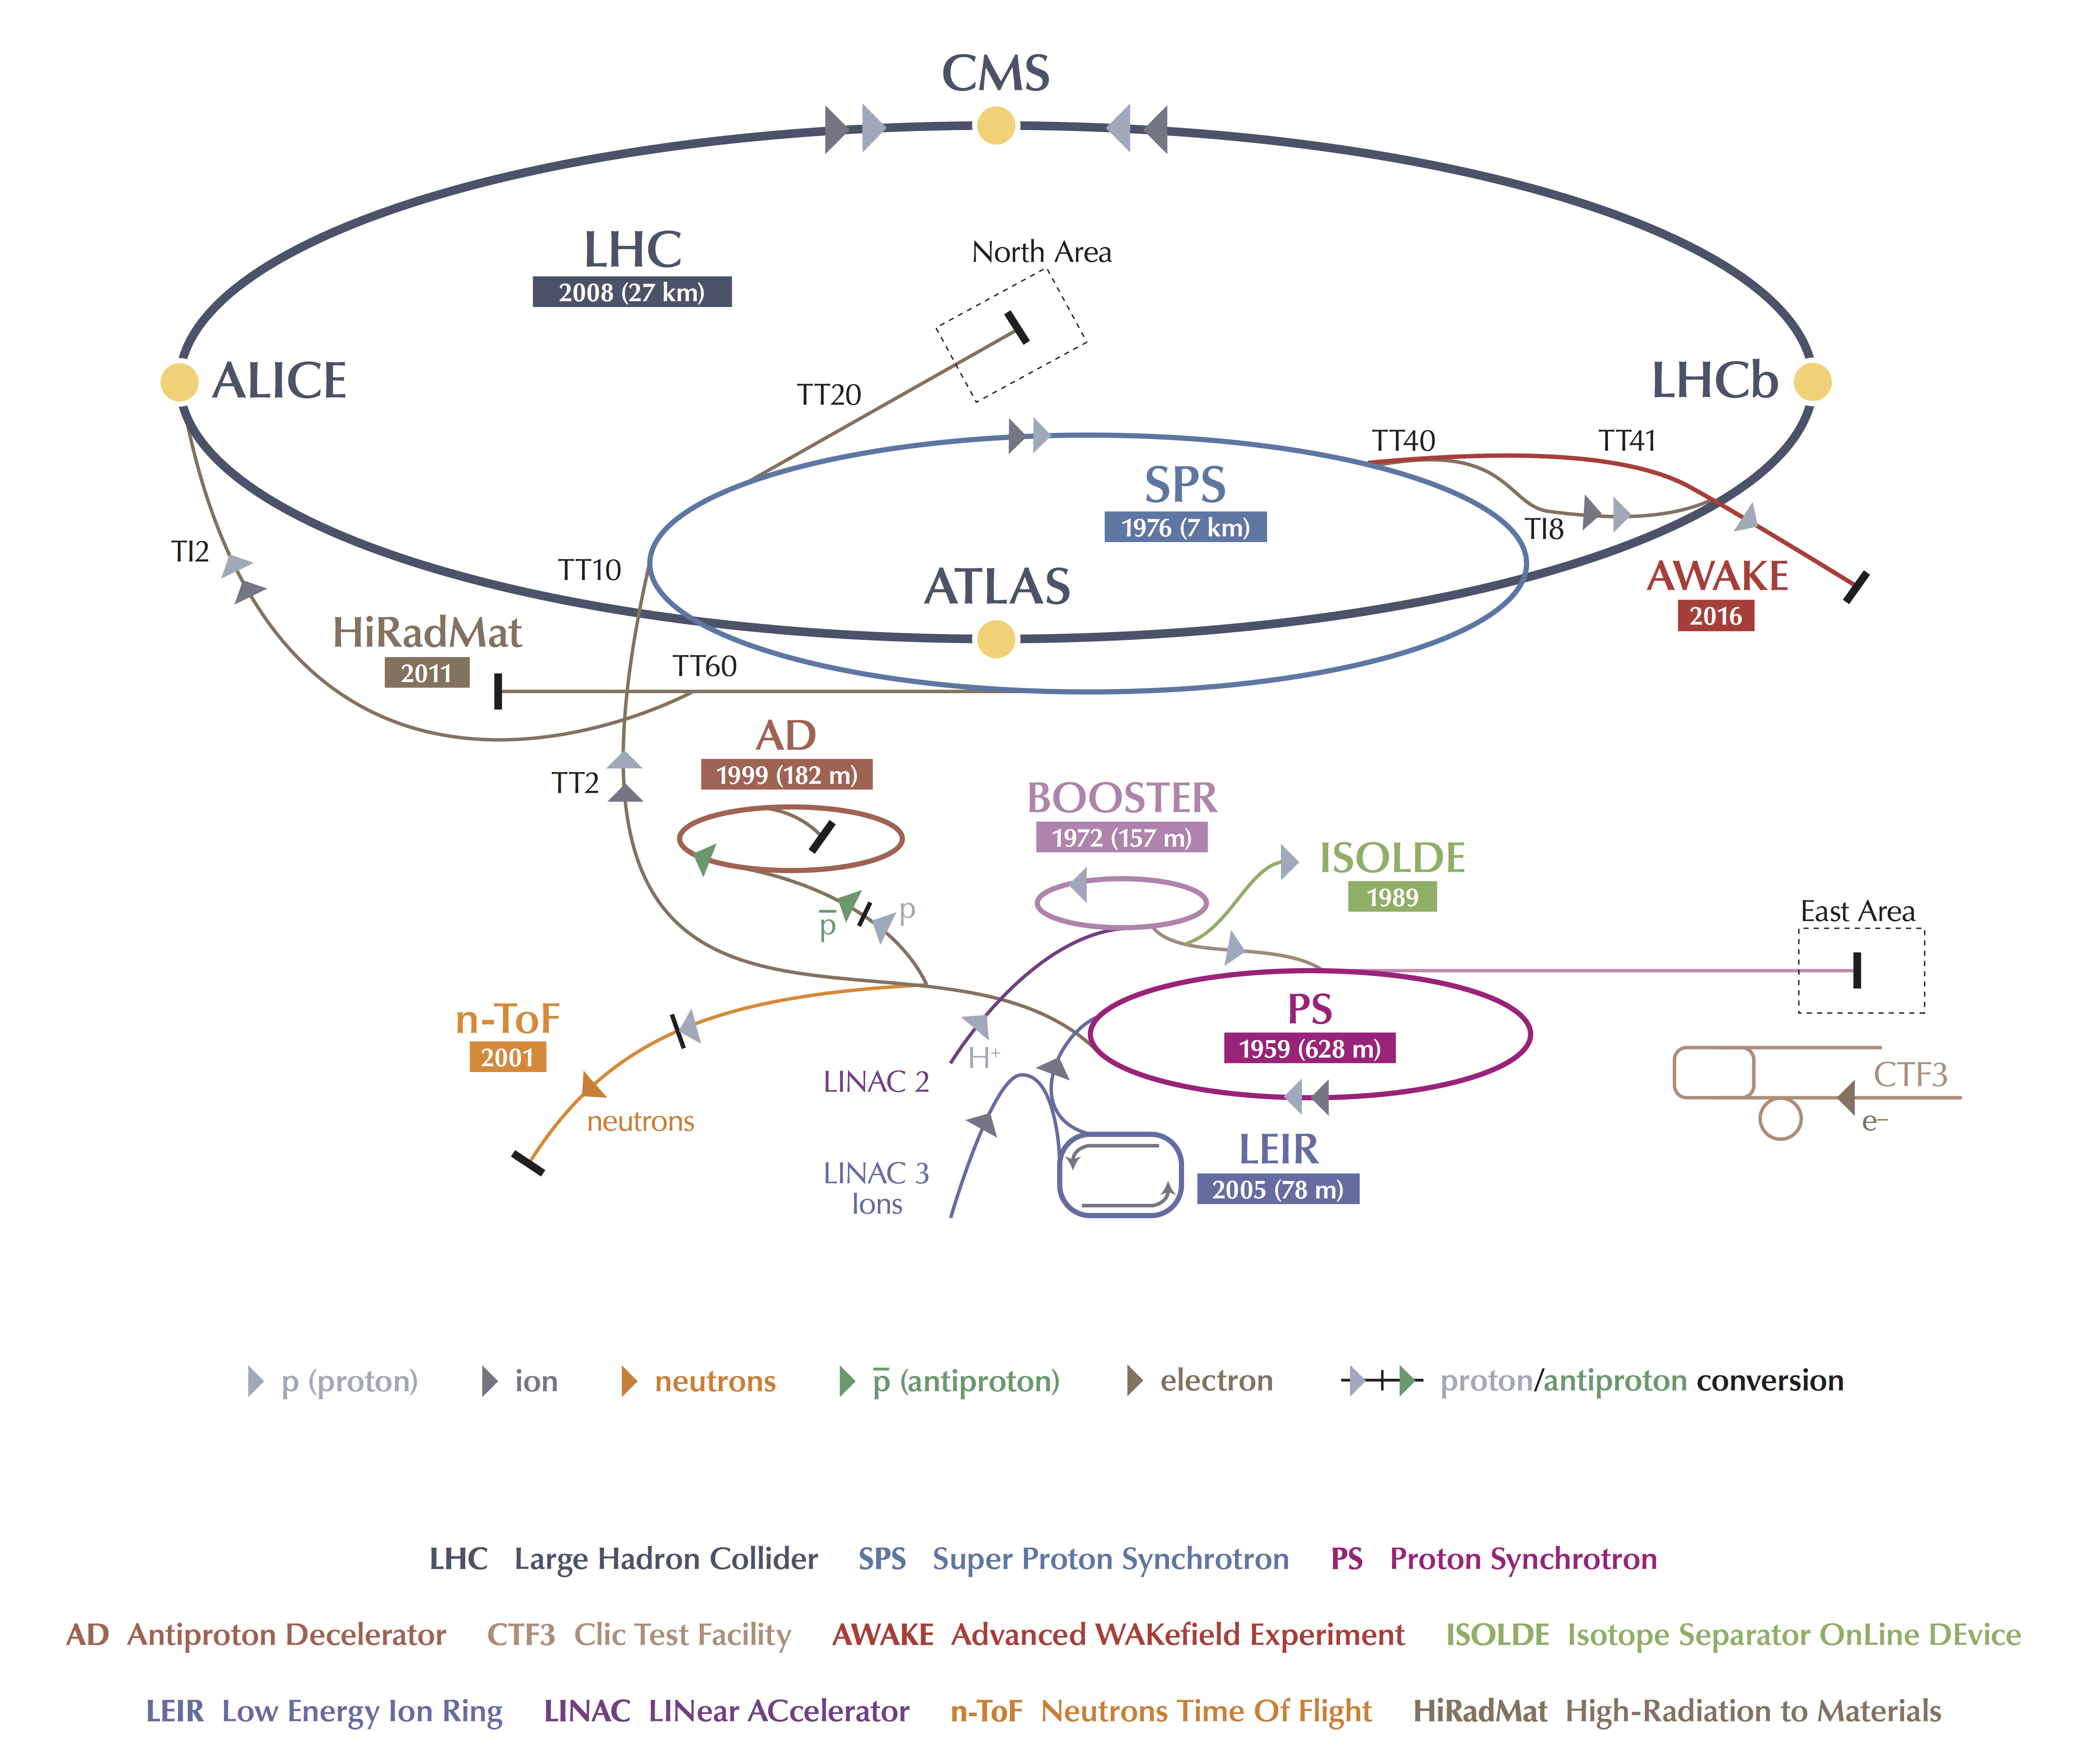
\includegraphics[width=\linewidth]{Figures/LHC/accelerator.jpg}
       \caption{Schematic of the CERN accelerator complex. The LHC is shown in dark grey and includes four interaction points: one each for the CMS, ATLAS, LHCb, and ALICE experiments. Prior to being injected into the LHC, the protons are accelerated through the Linear Accelerator 2 (Linac 2), the Proton Synchrotron Booster, the Proton Synchrotron (PS), and the Super Proton Synchrotron (SPS). Reprinted from Reference~\cite{CDS}.}
       \label{fig:accelerator}
\end{figure*}

\section{LHC tunnel and magnets}
\label{sec:tunnel}

Due to the prohibitive cost of building a new tunnel, the LHC uses the same tunnel as the one previously occupied by the Large Electron-Positron (LEP) Collider. This placed several constraints on the design of the accelerator. Because of the large synchrotron radiation losses that occur when accelerating light particles such as electrons, the LEP tunnel included eight straight sections where the electrons and positrons could be accelerated. For a hadron collider such as the LHC, however, the losses due to synchrotron radiation are less than 7 keV per rotation. The straight sections of the tunnel mean that the arced sections have a smaller radius of curvature $R$ than if the tunnel was perfectly circular. This directly affects the maximum attainable momentum $p$ of a particle with charge $q$ for a given magnetic field $B$:
\begin{equation}
B = \frac{p}{qcR}
\end{equation}

To reach the design energy $\sqrt{s} = 14$ TeV, the LHC dipoles must be able to operate at a magnetic field $B = 8.33$ TeV. This requires the magnets to be superconducting. The LHC includes 1232 dipole magnets that are cooled to 1.9 K using liquid helium. The solenoid of each magnet is made of stacked niobium-titanium (NbTi) filaments of thickness 6-7 $\mu$m. The LEP tunnel is too narrow (3.7 m radius) to fit two magnet systems and the associated cryogenics and insulation. Therefore, the LHC magnets use a ``twin-bore" design, where both of the beams are embedded in a single magnet system.

The LHC has only one accelerating sector. In the sector, there are eight superconducting RF cavities per beam that operate at a frequency of 400 MHz. The RF cavities add 485 keV per rotation. The beams consist of ``bunches" of protons with a spacing of 25 ns separating consecutive bunches. Each collision between two bunches is referred to as a bunch crossing. 

\section{Machine luminosity}
\label{sec:tunnel}

The number of events $N_{\mathrm{event}}$ produced every second for a particular process with cross section $\sigma_{\mathrm{event}}$ is given by
\begin{equation}
N_{\mathrm{event}} = L\sigma_{\mathrm{event}}
\end{equation}
where $L$ is the instantaneous luminosity of the collider. 

The instantaneous luminosity depends only on machine parameters: 
\begin{equation}
L = \frac{N_b^2 n_b f_{rev} \gamma_r}{4\pi\epsilon_n\beta\ast}F
\end{equation}
The variables in the above equation include the number of particles per bunch $N_b$, the number of bunches per beam $n_b$, the revolution frequency $f_{rev}$, and the relativistic factor $\gamma_r$. For the LHC, $n_b$ is 2808 for the nominal bunch spacing of 25 ns. The number of protons per bunch $N_b$ is limited to 1.15$\times 10^{11}$ by the nonlinear beam-beam interactions between protons at each IP. 

The normalized transverse beam emittance $\epsilon_n$ is a measure of the average spread of particles in the beam in position-momentum phase space. In the transverse direction the beam is assumed to have a Gaussian shape with width $\sigma$. The beta function is then given by $\beta = \sigma^2 /\epsilon$, and $\beta\ast$ refers to the value of the beta function at the interaction point. Finally, $F$ is a geometric factor that depends on the crossing angle at the IP. 

The design instantaneous luminosity of the LHC is 10$^{34}$ cm$^{-2}$ s$^{-1}$. This goal is only attainable because the LHC is a $p$-$p$ collider, rather than a $p$-$\bar{p}$ collider. During the 2016 data-taking period, the LHC met and surpassed its luminosity target, achieving a maximum value of 1.53$\times 10^{34}$ cm$^{-2}$ s$^{-1}$. This is almost double the maximum value of 7.7 $\times 10^{33}$ cm$^{-2}$ s$^{-1}$ that was achieved during Run I. The peak luminosity per day in 2016 is shown in Figure~\ref{fig:instLumi}. The measurement of instantaneous luminosity is described in more detail in Section~\ref{sec:lumi}. 

\begin{figure*}[h!]
	\centering
	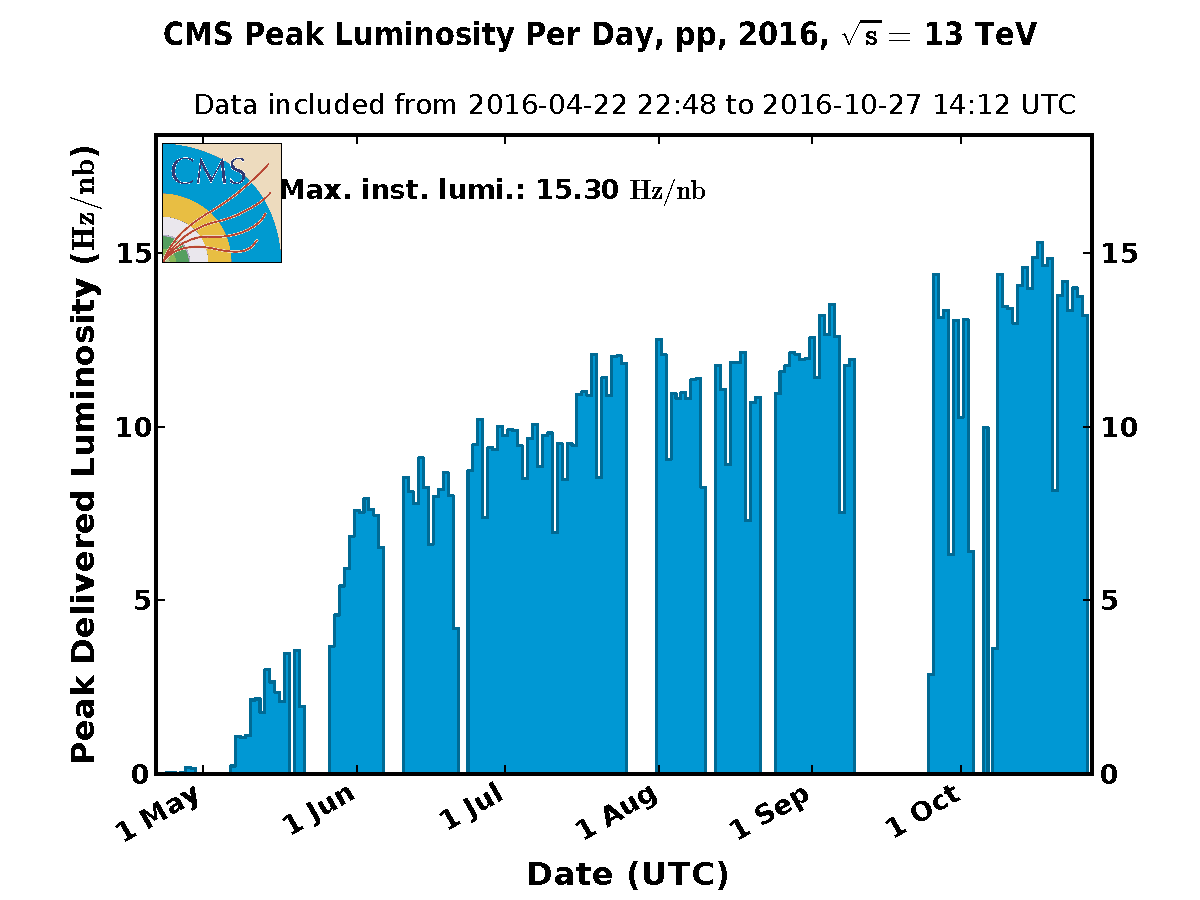
\includegraphics[width=\linewidth]{Figures/LHC/peak_lumi_per_day_pp_2016.pdf}
       \caption{Peak instantaneous luminosity per day achieved by the LHC during the 2016 data-taking period. 
       The maximum luminosity was 15.3 Hz/nb, or 1.53$\times 10^{34}$ cm$^{-2}$ s$^{-1}$. }
       \label{fig:instLumi}
\end{figure*}


%20 minutes to ramp the magnets down after abort
%Minimum LHC injection time is 16 minutes for PS into SPS into LHC
%20 minutes to make sure everything is okay.
%20 minutes to ramp back up

%Improvements between Run I and Run II: 
%https://press.cern/backgrounders/stronger-machine

%Three vacuum systems: 
%insulation vacuum for cryostat, insulation vacuum for helium,  10$^{-1}$ mb
%beam vacuum: more important. Affects beam lifetime (how long one fill lasts) and background from protons scattering off other nonsense in the beam. Must be better than $10^{-10}$ mb at room temp
%"below 1015H2m?3 at cryogenic temperatures (expressed as a gas density normalized to hydrogen, taking into account the ionization cross sections for each gas species)."


  \chapter{CMS DETECTOR}
\label{chap:Detector}

The Compact Muon Solenoid (CMS) detector is a multi-purpose detector designed to accurately measure the energy and momentum of all particles produced in proton-proton or heavy ion collisions. Figure~\ref{fig:CMS} shows a schematic of the detector as a whole. The CMS detector is 21.6 m long, 14.6 m in diameter, and weighs 12500 t. 
Moving radially outward from the interaction point, the sub-detectors are the silicon pixel and strip tracker (Section~\ref{sec:Tracker}), the electromagnetic calorimeter (Section~\ref{sec:ECAL}), the hadron calorimeter (Section~\ref{sec:HCAL}), and the muon system (Section~\ref{sec:Muon}). For a full description of the CMS detector, see Reference~\cite{Chatrchyan2008zzk}. 

\begin{figure}[h!]
	\centering
	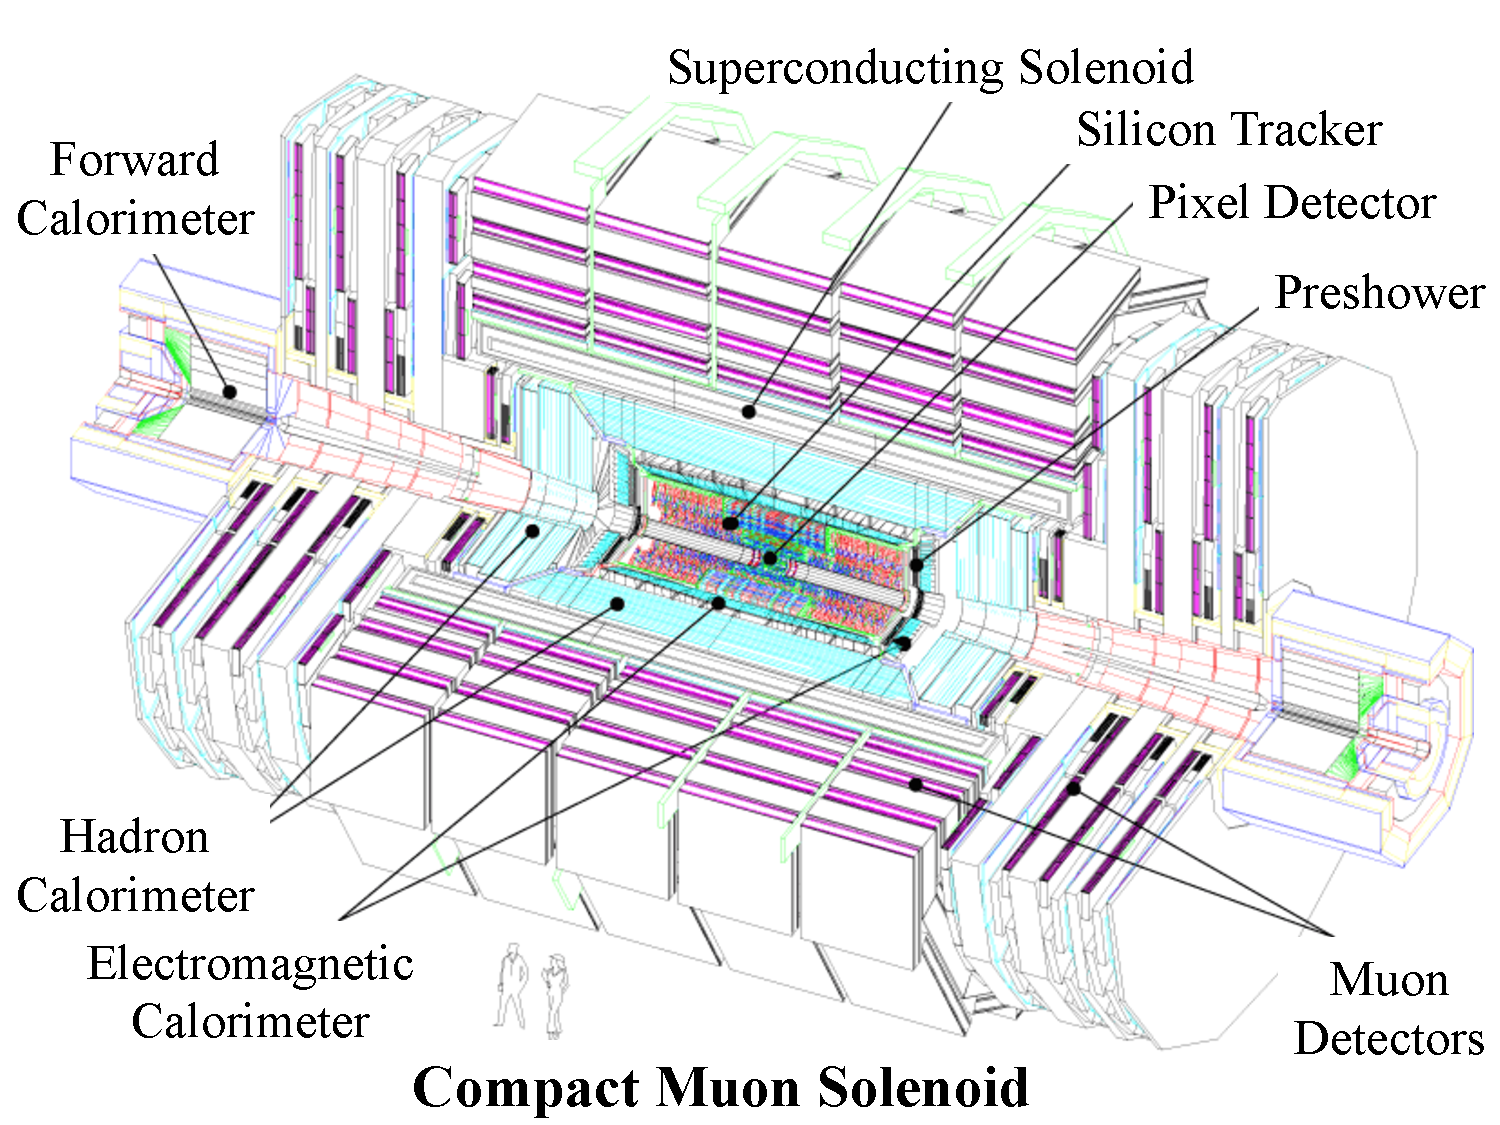
\includegraphics[width=0.8\textwidth]{Figures/Detector/cms_labelled.pdf}
       \caption{Schematic of the CMS detector.
	}
   	\label{fig:CMS}
\end{figure}

%%%%%%%%%%%%%%%%%%%%%%%%%%%%

\section{Coordinate system}
\label{sec:coordinates}
The origin of the CMS detector coordinate system is located at the nominal collision point. The $z$-axis is oriented along the beam direction, with the positive $z$-axis pointing in the counter-clockwise direction when viewing the LHC from above. The $y$-axis points vertically upward, and the $x$-axis points toward the center of the LHC. The $xy$-plane is referred to as the transverse plane.

Due to the nature of particle collisions, however, Cartesian coordinates are often not the most convenient. Because protons are not elementary particles, it is actually the individual quarks or gluons within the proton that interact during the collision. This means that the collision will not be at rest in the lab frame, but will have some non-zero velocity along the $z$-axis. To deal with this, it is beneficial to use coordinates that are invariant under boosts in the $z$-direction. CMS follows the particle physics convention of describing the position of a particle in terms of its transverse momentum, azimuthal angle, and pseudorapidity. The transverse momentum \pt is defined as the magnitude of the momentum in the $xy$-plane. The azimuthal angle $\phi$ is defined in the transverse plane, with $\phi  = 0$ corresponding to the positive $x$-axis. Finally, the pseudorapidity is defined as $\eta = -\ln{\tan{ (\theta / 2 )} } $, where the polar angle $\theta$ is measured from the $z$-axis. 

%%%%%%%%%%%%%%%%%%%%%%%%%%%%

\section{Superconducting solenoid}
\label{sec:magnet}

One of the most important components of the CMS detector is the superconducting solenoid that provides the bending power necessary to precisely measure the momentum of all charged particles produced in the collision. The solenoid is a 4-layer niobium-titanium coil embedded in aluminum and aluminum alloy. The magnet is located between the calorimeters and the muon system. It is 12.5 m long and has an inner diameter of 6 m. It is capable of producing magnetic fields up to 4 T, although the magnet is generally operated at 3.8 T to prolong its lifetime. At full current, the magnet has a stored energy of 2.6~GJ. A 12,000 ton steel yoke made up of 5 wheels in the barrel and 3 endcap disks serves to return the magnetic flux. The solenoid is suspended in a vacuum cryostat and cooled to 4.5 K with liquid helium. A detailed description of the CMS magnet can be found in Reference~\cite{magnetTDR}. Figure~\ref{fig:magnet} shows the calculated magnetic field in a longitudinal slice of the CMS detector.

\begin{figure*}[h!]
	\centering
	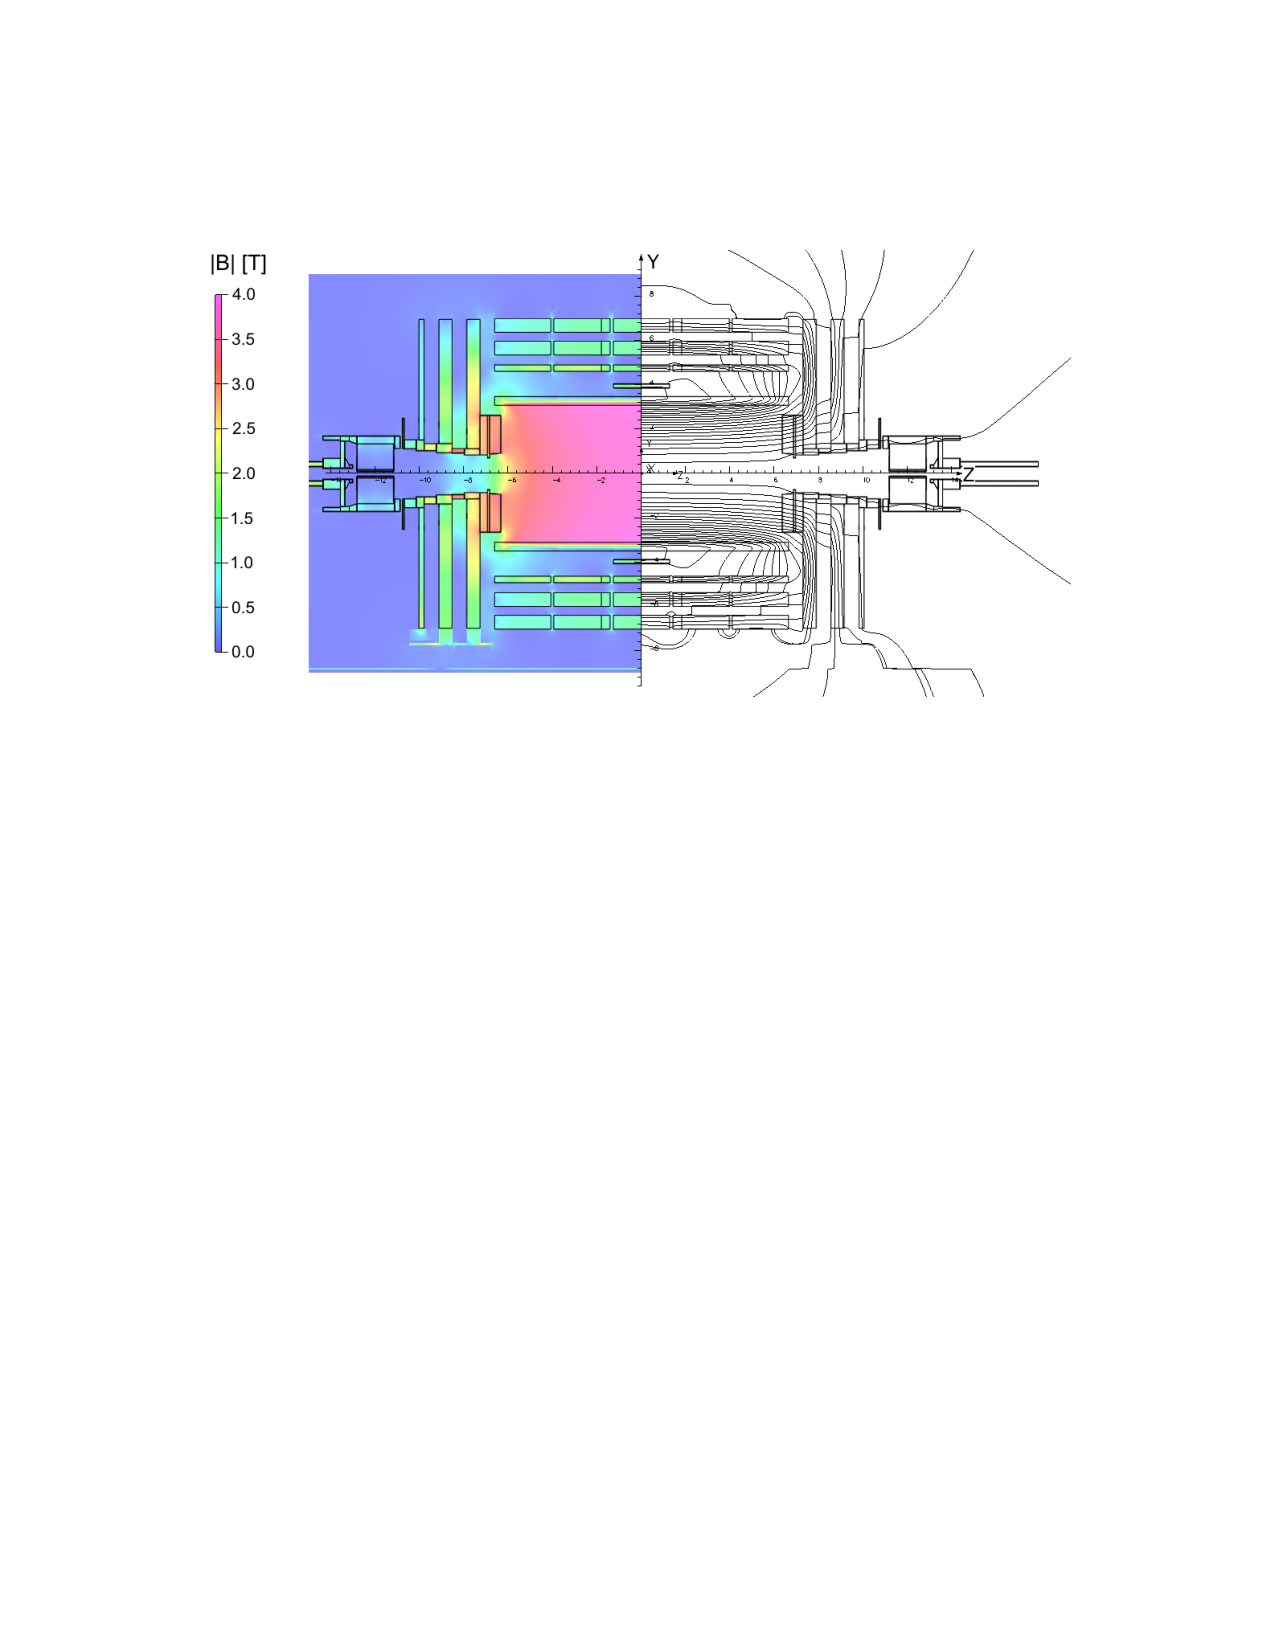
\includegraphics[width=\linewidth]{Figures/Detector/magnet.pdf}
       \caption{Calculated magnetic field $|\vec{B}|$ for a longitudinal slice of the CMS detector when operated at a central magnetic flux density of 3.8 T. In the right-hand portion of the figure, each magnetic field line represents a magnetic flux step of 6 Wb. Reprinted from Reference~\cite{CMSMagnetField}.}
       \label{fig:magnet}
\end{figure*}

%%%%%%%%%%%%%%%%%%%%%%%%%%%%

\section{Tracker}
\label{sec:Tracker}

The innermost sub-detector is the silicon tracker~\cite{trackerTDR,trackerTDRAddendum}. The tracker must provide enough information to accurately reconstruct the trajectories of charged particles to a high level of precision. This is accomplished through the use of silicon semiconductors, which rely on the properties of p-n junctions to detect charged particles. A p-n junction is created by bringing a p-type semiconductor into contact with an n-type semiconductor. For p- and n-type semiconductors, the crystal lattice of the semiconductor is doped to either donate or accept extra electrons, respectively. In a p-n junction, the extra electrons in the n-type semiconductor migrate and combine with the electron holes in the p-type semiconductor. This creates a depletion region in the center of the crystal. Charged particles passing through the depletion region will create electron-hole pairs that move towards either end of the junction when an external electric field is applied. The resulting current is proportional to the energy deposited in the detector.

The overall dimensions of the tracker are 5.6 m long and 1.2 m in radius. The full tracking system is cylindrical in shape and is comprised of a barrel and two endcaps, each of which is split into layers of silicon pixel detectors and layers of silicon micro-strip detectors. In total, there are 48 million $150\times100~\mu$m pixels and 9.6 million strips that are between 80 and 180 $\mu$m wide. Figure~\ref{fig:TrackerLayout} shows a schematic drawing of the layout of the tracker subsystems. For charged hadrons with transverse momentum \pt less than 20 GeV, the \pt can be measured with a resolution of $1\%$. 

\begin{figure*}[h!]
	\centering
	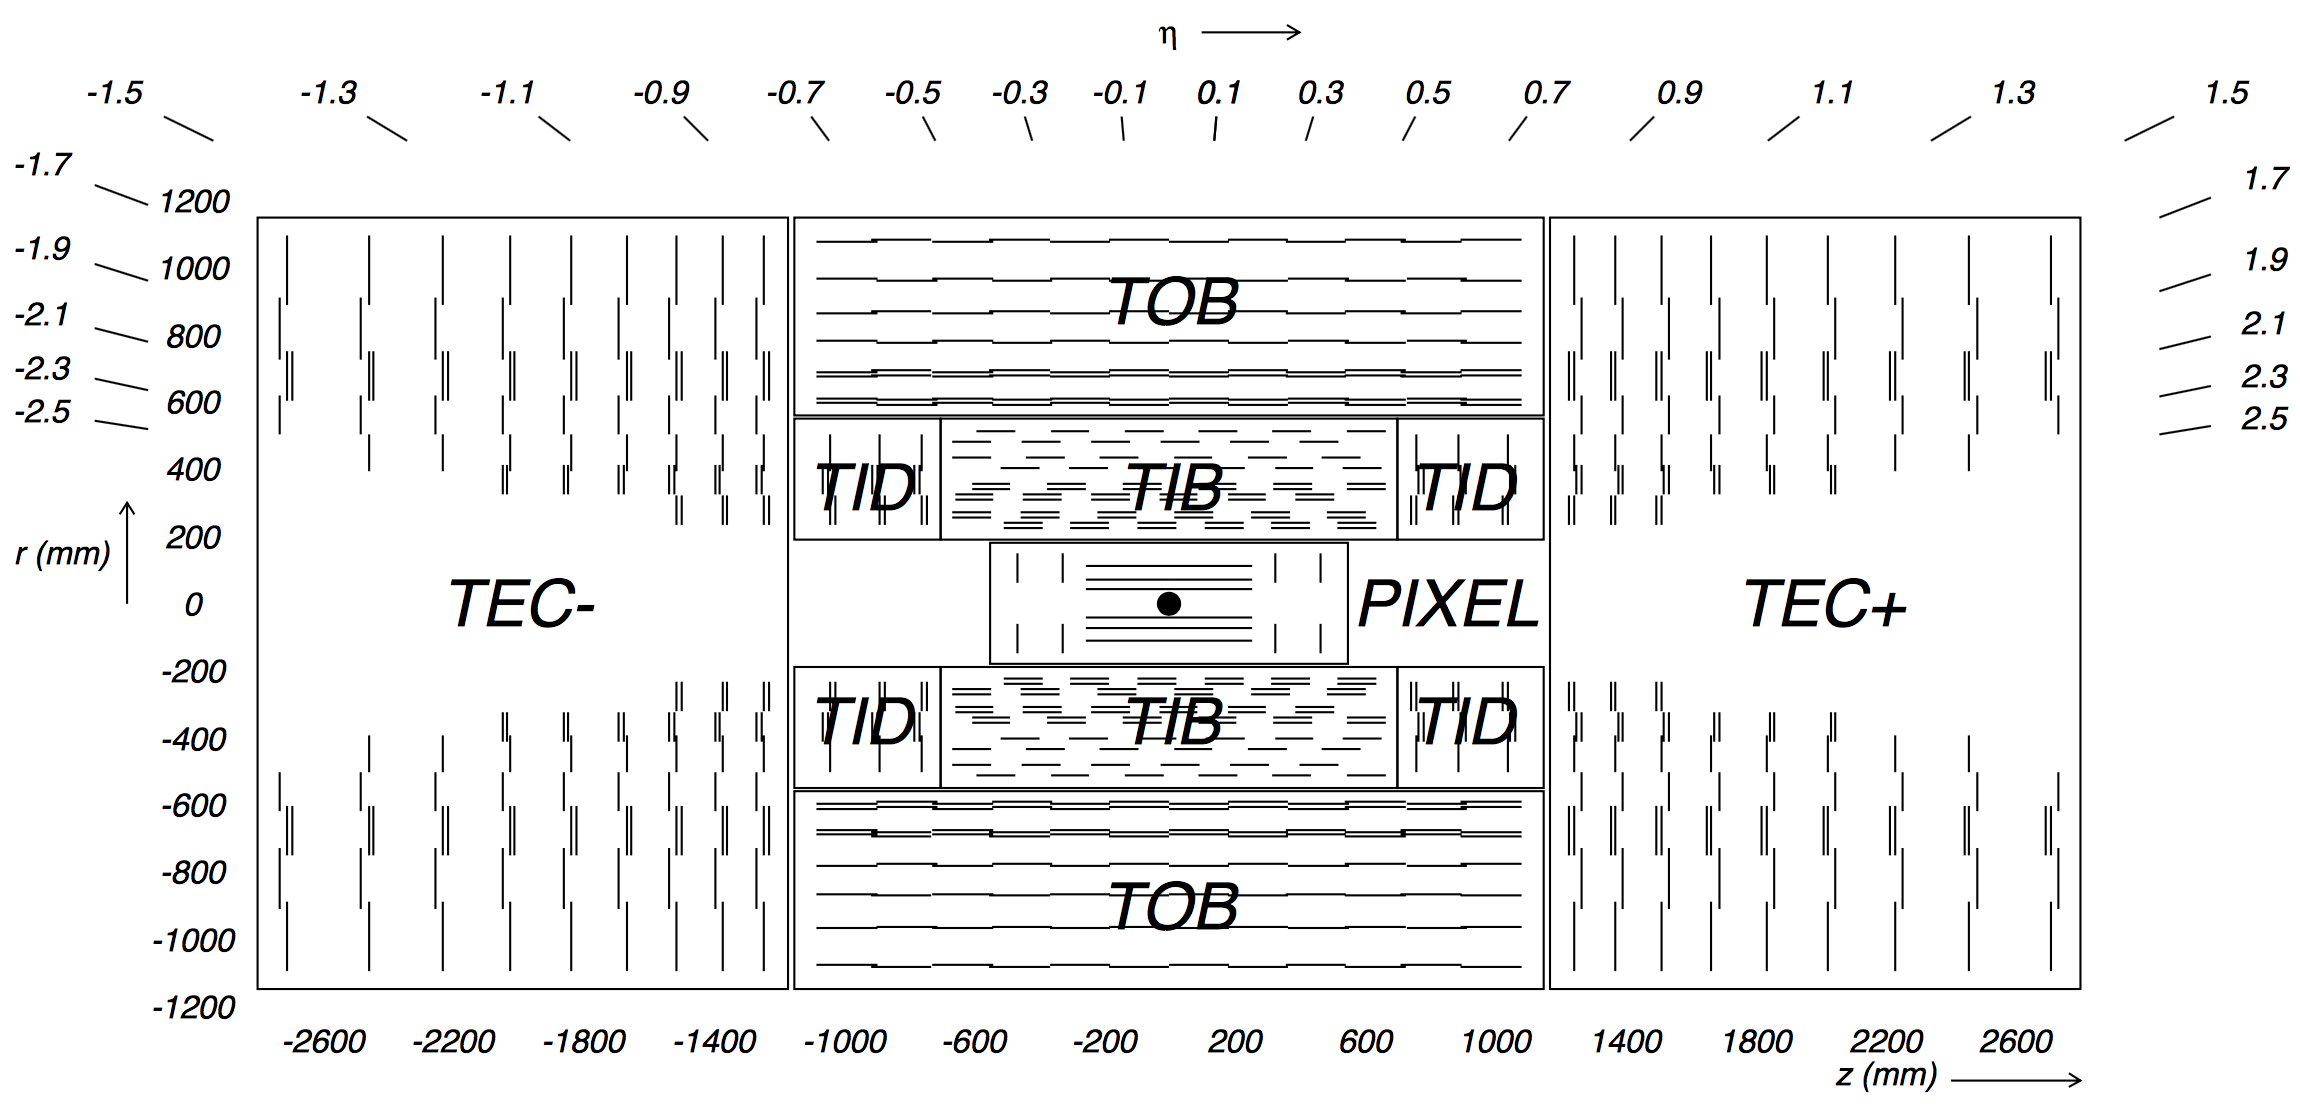
\includegraphics[width=\linewidth]{Figures/Detector/tracker_layout.png}
       \caption{Schematic of the CMS tracker system. Detector modules are represented by single lines, and back-to-back modules are represented by double lines. The strip tracker is further divided into the Tracker Inner/Outer Barrel (TIB/TOB), Tracker Inner Disk (TID) and the Tracker Endcap (TEC). Reprinted from Reference~\cite{Chatrchyan2008zzk}.}
   	\label{fig:TrackerLayout}
\end{figure*}

\subsection{Pixel detectors}
\label{sec:TrackerPixel}

Due to the high occupancy of the tracker within 10 cm of the beam pipe, pixel detectors rather than strip detectors are used as the innermost layers of the tracker. Three layers in the barrel and two disks of pixel detectors in the endcap give three high-precision points for every charged particle moving away from the interaction point. The small pixel size of $150\times100~\mu$m is critical for accurate secondary vertex reconstruction, for forming seed tracks used for high level triggering (see Chapter~\ref{chap:Trigger}), and for the reconstruction of charged particles in the event (see Chapter~\ref{sec:EventReconstruction}). The three barrel layers are 53 cm long and are located at mean radii of 4.4, 7.3 and 10.2 cm. The endcap modules extend radially from 6 to 15 cm and are placed on each side at $z=\pm34.5$ and $z=\pm46.5$~cm. The endcaps extend the coverage of the sub-detector to $|\eta|~<~ 2.5$. 
%Yutaro: An interpolation of the signal amplitudes gives a spacial resolution of 15-20 mum, (because charge is shared between several pixels due to the geometry and the magnetic field)

\subsection{Strip detectors}
\label{sec:TrackStrip}
Moving radially beyond the pixel detectors are the silicon strip trackers. These operate on the same basic principles as the pixel detectors, but each silicon strip is 10 cm $\times~80~\mu$m, giving a precise position measurement along one dimension only. In the barrel, the strips run parallel to the $z$-axis with a pitch, or spacing between strips, between 80 and 183 $\mu$m. Strips in the endcaps are aligned radially with a pitch between 100 and 184 $\mu$m. In total there are 10 layers of strip sensors in the barrel and 12 layers in the endcaps.

The tracker has a spatial resolution of 25-50 $\mu$m perpendicular to the strip direction. In order to improve the precision of the detector in the direction parallel to the strips, several of the layers are arranged in pairs. By aligning the second layer 100 mrad off from the strips in the first layer, a spatial resolution of 230 to 530 $\mu$m can be achieved. These back-to-back modules are represented by double lines in Figure~\ref{fig:TrackerLayout}.

%Yutaro: paragraph on the alignment system for the strips.

%%%%%%%%%%%%%%%%%%%%%%%%%%%%

\section{Electromagnetic Calorimeter (ECAL)}
\label{sec:ECAL}

Beyond the tracker is the electromagnetic calorimeter (ECAL), the most important sub-detector for this analysis~\cite{ECAL_TDR,ECAL_TDRAddendum}. The ECAL measures the energies deposited by photons and electrons when they are stopped by the detector. For energies above 10 MeV, electrons lose energy primarily through the production of photons in bremsstrahlung. Photons lose energy through the production of $e^+e^-$ pairs \cite{Calo}. Therefore, when an energetic electron or photon is incident on one of the crystals of the ECAL, the result is an electromagnetic cascade (``shower") of photons and electrons with successively lower energies.

The CMS ECAL is designed to contain the full electromagnetic shower from electrons and photons with initial energies as high as a few TeV. It is a homogeneous calorimeter made with 75,848 scintillating lead tungstate PbWO$_4$ crystals. The ECAL is divided into a barrel region (EB) covering $|\eta| < 1.479$ and two endcap regions (EE) covering $1.479 < |\eta| < 3.0$.  Each region includes a single layer of PbWO$_4$ crystals. In the barrel, the crystals have a truncated pyramidal shape with a radial depth of 23 cm. The front face of the crystal has dimensions 22 $\times$ 22 mm$^2$, and the rear face has dimensions 26 $\times$ 26 mm$^2$. In the endcap, the crystals are 22 cm long and have a cross-section of 28.62 $\times$ 28.62 mm$^2$ on the front face and 30.0 $\times$ 30.0 mm$^2$ on the rear face. 

Lead tungstate is an inorganic scintillator. The passage of charged particles produce electron-hole pairs in the conduction and valence bands of the material, and light is emitted when the electrons return to the valence band. There are several properties of PbWO$_4$ that make it an ideal choice for the scintillating material of the CMS ECAL. Its Moli\`{e}re radius, defined as the radius of a cylinder containing 90\% of the shower's energy deposition, is only 2.2 cm, allowing for excellent position resolution and separation between showers. The latter is particularly important when trying to distinguish photons from isolated $\pi^0\rightarrow\gamma\gamma$ decays. The fast response time of lead tungstate is also critical. Approximately 80\% of the light is emitted within 15 ns \cite{Calo}, making it possible for each particle to be assigned to the correct bunch crossing. 

Another positive feature of PbWO$_4$ is that it is dense enough (8.3 g/cm$^3$) that the ECAL can fit into a relatively compact area. The depth of material that is needed is quantified by looking at the radiation length of the material ($\chi_0$). The radiation length is the average distance an electron needs to travel to reduce its energy by a factor 1/$e$. The radiation length of PbWO$_4$ is 0.89 cm, which means 24.7 $\chi_0$ fit in the 22 cm radial distance of each EB crystal.

Finally, the last characteristic of PbWO$_4$ that put it ahead of other inorganic scintillators is its radiation hardness. Nuclear reactions caused by prolonged exposure to severe radiation conditions can cause defects in the crystals of inorganic scintillators. This affects the transparency of the crystals, leading to a degradation in the crystal response. This is shown in Figure~\ref{fig:ecal_response} for the 2011, 2012, 2015, and 2016 data-taking periods. To correct for this effect, each crystal is illuminated with laser light. Part of the light is redirected to a silicon photodiode off the detector for a reference measurement. This correction is important both for long-term damage as illustrated in Figure~\ref{fig:ecal_response}, but also for the fast component of the radiation damage that changes the crystal response over the course of a single LHC fill.

\begin{figure*}[h!]
	\centering
	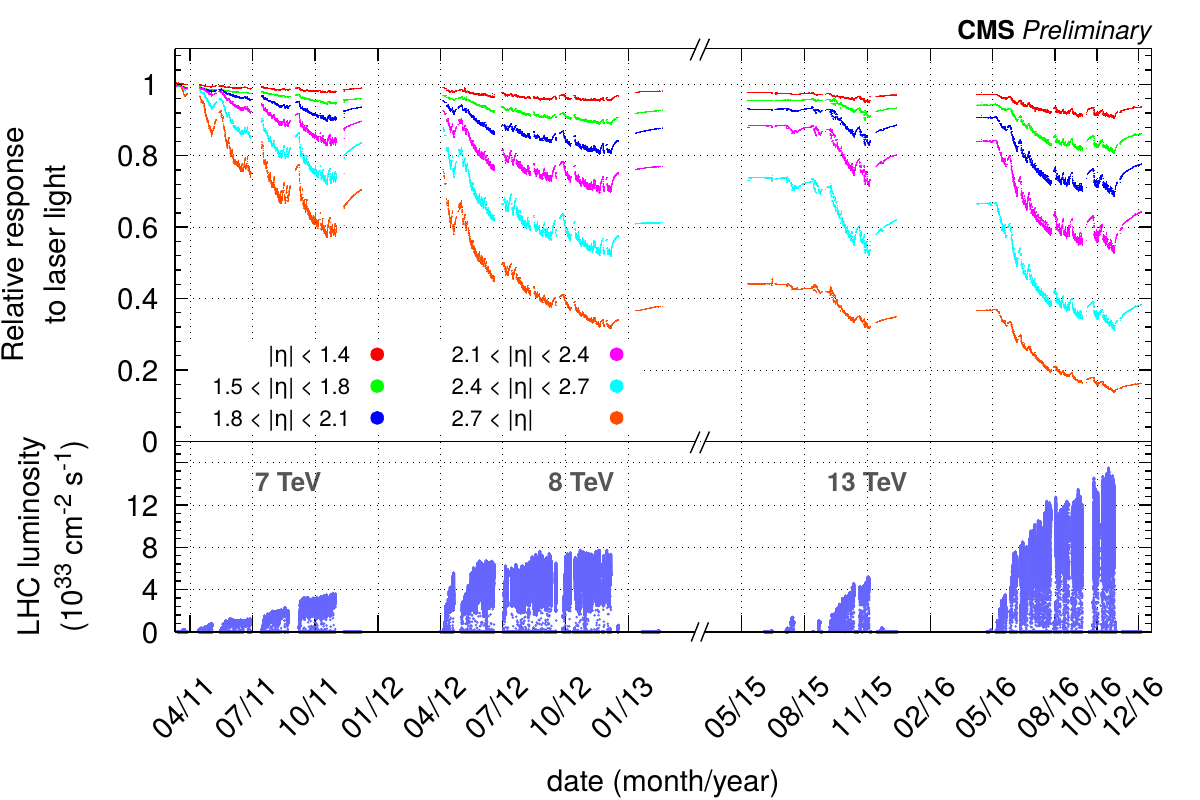
\includegraphics[width=\linewidth]{Figures/Detector/ecal_response.png}
       \caption{ Relative response of the ECAL crystals for the 2011 to 2016 data-taking periods.
       The average observed change in response is up to 10\% in the barrel and 50\% for $|\eta|$ < 2.5. 
       The bottom plot shows the instantaneous luminosity delivered during this period. The crystals recovered 
       some, but not all, of their response during 2013-2014 Long Shutdown 1. Reprinted from Reference~\cite{ECALDPGtwiki}.}
   	\label{fig:ecal_response}
\end{figure*}


The downside to PbWO$_4$ is that it has a relatively low light yield of only 2 photoelectrons per MeV of incident energy. This makes the electronics used to collect the signal especially important. The crystal itself acts as an optical waveguide, and the scintillation light is internally reflected until it reaches the photodetectors glued directly onto the rear face of the crystal. Avalanche photodiodes (APD) are used in the barrel, and vacuum phototriodes (VPT) are used in the more radioactive endcap region. Both of these were chosen to be able to operate within the 3.8 T magnetic field, and both increase the gain by a factor of approximately 1000.
The signal then goes to a Multi-Gain Preamplifier (MGPA), which dynamically changes the gain based on the energy of the incident particle. 
Temperature control of the PbWO$_4$ crystals and the attached APDs is crucial to maintaining an excellent resolution. The crystal response and APD gain change by approximately 2.2\% and 2.4\% per $^\circ$C, respectively. 

The last sections of the ECAL system are two pre-shower detectors located in front of the EE. The pre-shower detector is designed to improve the spatial resolution of the ECAL, so that the two photons from $\pi^0\rightarrow\gamma\gamma$ decays can be distinguished. Each pre-shower detector consists of alternating strips of lead and silicon detectors. The lead forces the photons to interact, and the silicon detector measures the electrons and positrons produced in the shower with high granularity. The pre-shower detector achieves a spatial resolution of 2 mm, compared to the 3 cm resolution of the EB and EE. 


%%%%%%%%%%%%%%%%%%%%%%%%%%%%

\section{Hadron calorimeter (HCAL)}
\label{sec:HCAL}
The Hadron calorimeter (HCAL) is the next sub-detector after the ECAL. It is a brass sampling calorimeter, with alternating layers of plastic scintillator and brass absorbers. 
Heavy particles such as hadrons interact with the brass layers, and the scintillation light from the nuclear showers is collected with wavelength-shifting optical fibers embedded in the plastic scintillator. The light is then guided to pixelated hybrid photodiodes and electronics that amplify the signal. Figure~\ref{fig:HCAL_layout} shows a longitudinal slice of the full HCAL system. 

%Heavy particles such as hadrons interact with the brass layers, and the energy of the resulting nuclear shower is detected in the plastic scintillators. 
%When a charged particle passes through the scintillator, the scintillation light is collected with wavelength-shifting optical fibers. 

\begin{figure*}[h!]
	\centering
	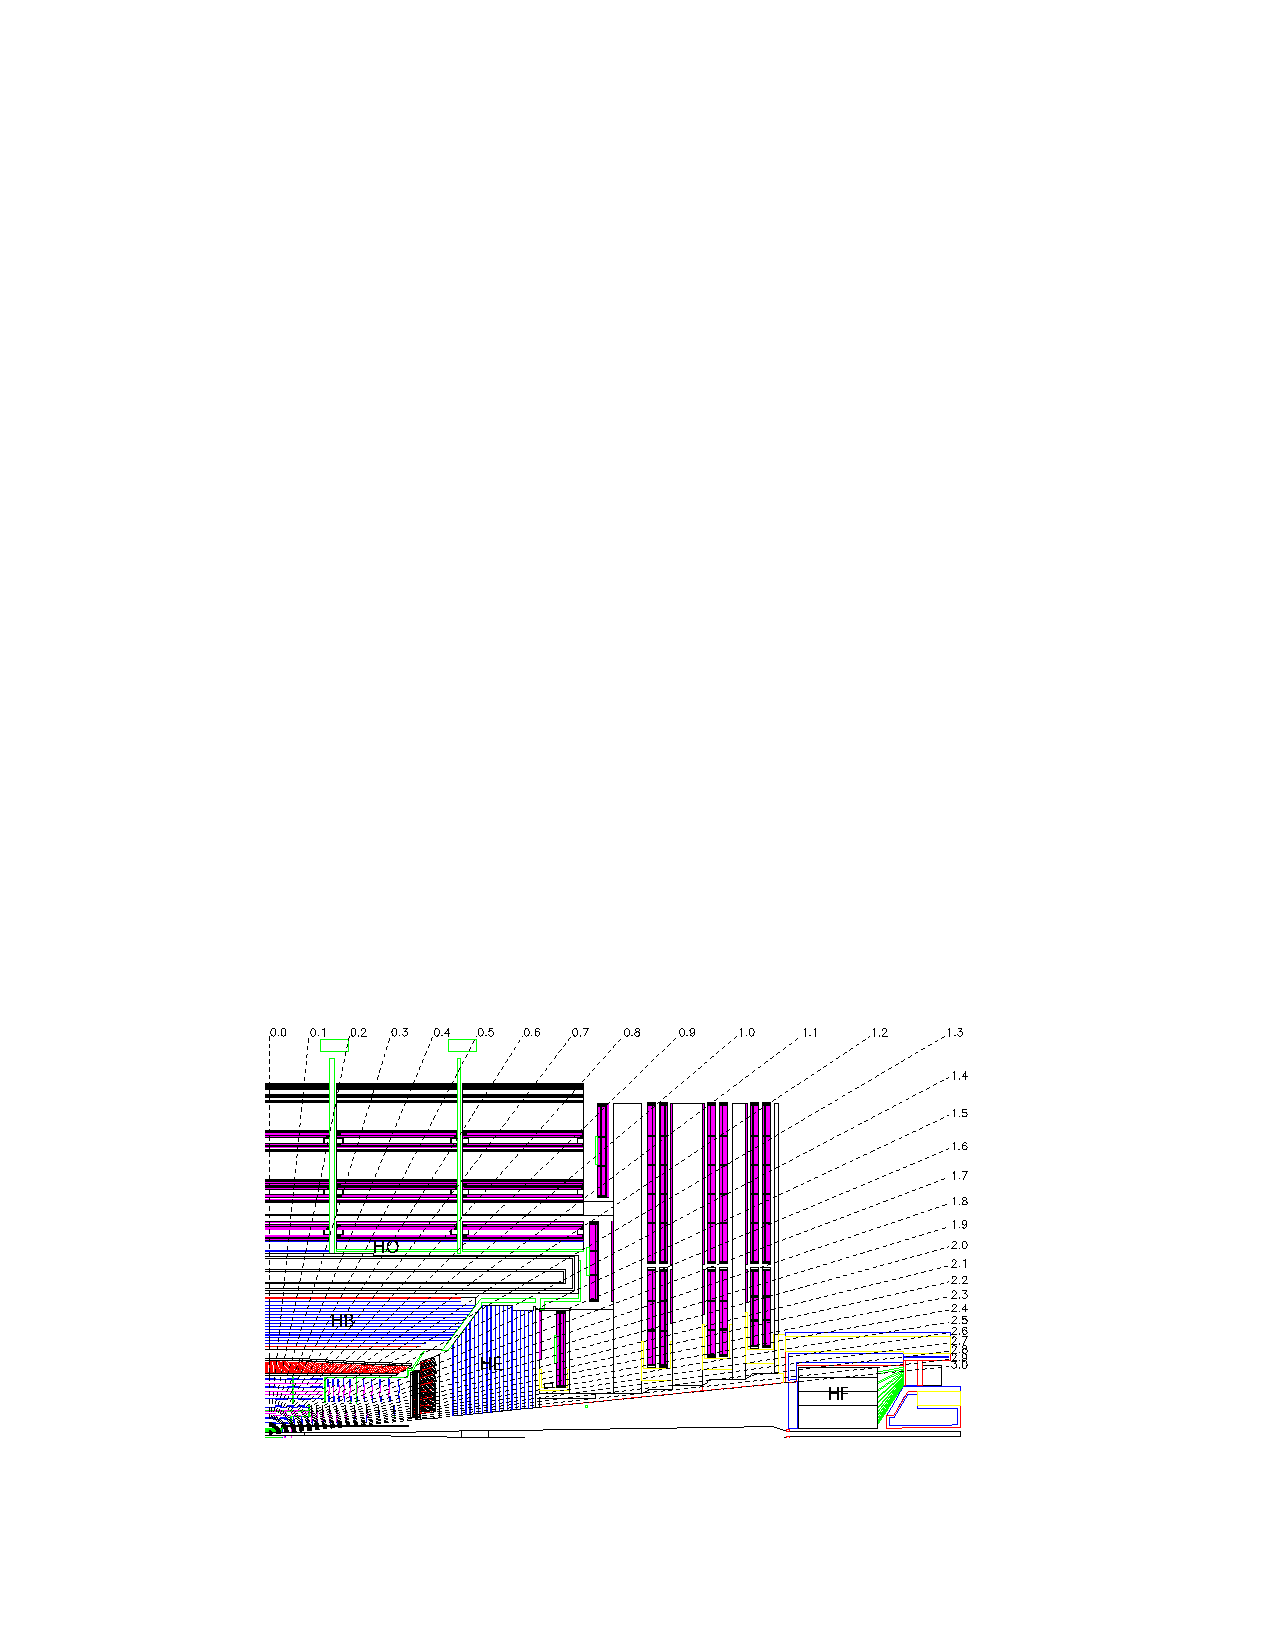
\includegraphics[width=\linewidth]{Figures/Detector/HCAL_layout.pdf}
       \caption{Longitudinal slice of the CMS HCAL, including the barrel HCAL (HB), outer HCAL (HO), endcap HCAL (HE), and forward HCAL (HF). The dashed lines represent lines of constant pseudorapidity. Reprinted from Reference~\cite{Chatrchyan2008zzk}.}
       \label{fig:HCAL_layout}
\end{figure*}

There are 17 scintillator layers in the barrel of the HCAL (HB), which extends radially from 1.77 to 1.95 m and to a pseudorapidity $|\eta| = 1.3$. The first and last layers of absorber are made of steel rather than brass for structural reasons. The scintillation layers are divided into tiles with area $\Delta\phi \times \Delta\eta = 0.87 \times 0.87$. The tiles are further organized into towers that each get a single readout channel. The outer HCAL (HO) is located outside the solenoid and serves to increase the thickness of the calorimeter. 

The HCAL endcap (HE) covers the pseudorapidity range $1.3 < |\eta| < 3$. There are 17 layers of plastic scintillator and 18 layers of absorber in the HE. For $|\eta| < 1.6$, the tile size is the same as those in the barrel, and for $|\eta| >1.6$ the tile size is reduced to $\Delta\phi \times \Delta\eta = 0.17 \times 0.17$. Depending on the pseudorapidity, there are two or three readout channels per tower.
 
The last part of the HCAL system is the forward HCAL (HF) that covers the pseudorapidity range from $3 < |\eta| < 5.2$. Charged particles are detected via Cherenkov radiation in quartz fibers planted in the steel absorber. The quartz fibers were chosen to be able to withstand the high radiation levels of particles emitted close to the beam pipe. 
All three segments of the HCAL are calibrated using radioactive sources $^{136}$Cs or $^{60}$Co mounted on the tip of a moving wire. The radioactive sources produce photons at known energies, allowing for an absolute calibration of each scintillator. 

Because most of the energy from the nuclear showers is deposited in the absorbers rather than the scintillation material, 
the HCAL naturally has a lower energy resolution than the ECAL . In addition, nuclear showers might start 
before particles even reach the HCAL, or charged particles might deposit energy in the ECAL via bremsstrahlung. 
The mean distance travelled by a hadronic particle before undergoing 
an inelastic nuclear interaction is known as the nuclear interaction length. 
The radial depth of the ECAL corresponds to 1.1 nuclear interaction lengths, and
in the HCAL there are 5.82 interaction lengths at $|\eta|=0$ and 10.6 interaction lengths at $|\eta|=1.3$. 


%The relative energy resolution of the two calorimeters together is $\Delta\mathrm{E}/\mathrm{E} \approx 100\% / \sqrt{\mathrm{E}} $. 
%look up energy resolution
%references?
%this is old, but might work https://arxiv.org/pdf/0911.4991.pdf
%conference proceeding http://home.fnal.gov/~chlebana/CMS/PAS/HCALPerformance.pdf


%%%%%%%%%%%%%%%%%%%
\section{Calorimeter performance}
In general, the energy resolution $\sigma/E$ of a calorimeter can be modeled with the following equation where $\oplus$ is used to represent summing in quadrature \cite{Calo}:
\begin{equation}
\frac{\sigma}{E} = \frac{a}{\sqrt{E}} \oplus \frac{b}{E}  \oplus c 
\end{equation}
The first term is a stochastic term that takes into account random fluctuations in the amount of deposited energy for a particle with incident energy $E$. Homogeneous detectors like the ECAL have an excellent intrinsic resolution and a very small stochastic term. Sampling calorimeters such as the HCAL, on the other hand, have larger stochastic terms because the number of charged particles that hit the active layers varies from shower to shower.

The $b/E$ term represents electronic noise from the equipment that is used to collect the signal. This term can depend sensitively on the temperature of the electronics, as already mentioned for the EB APDs. Maximizing the energy yield helps improve this contribution to the energy resolution. The final term is constant and covers any irregularities in the detector response. This can include variations between ECAL crystals, radiation damage effects, or differences in response due to temperature gradients across the detector.

The resolution of the ECAL as measured using $Z\rightarrow ee$ events in the 2015 CMS dataset is shown in Figure~\ref{fig:ecal_resolution}. For the central region of EB. the electron energy resolution is better than 2\%/E. The energy resolution of objects in the HCAL will be described in more detail in Chapter~\ref{sec:EventReconstruction}.

\begin{figure*}[h!]
	\centering
	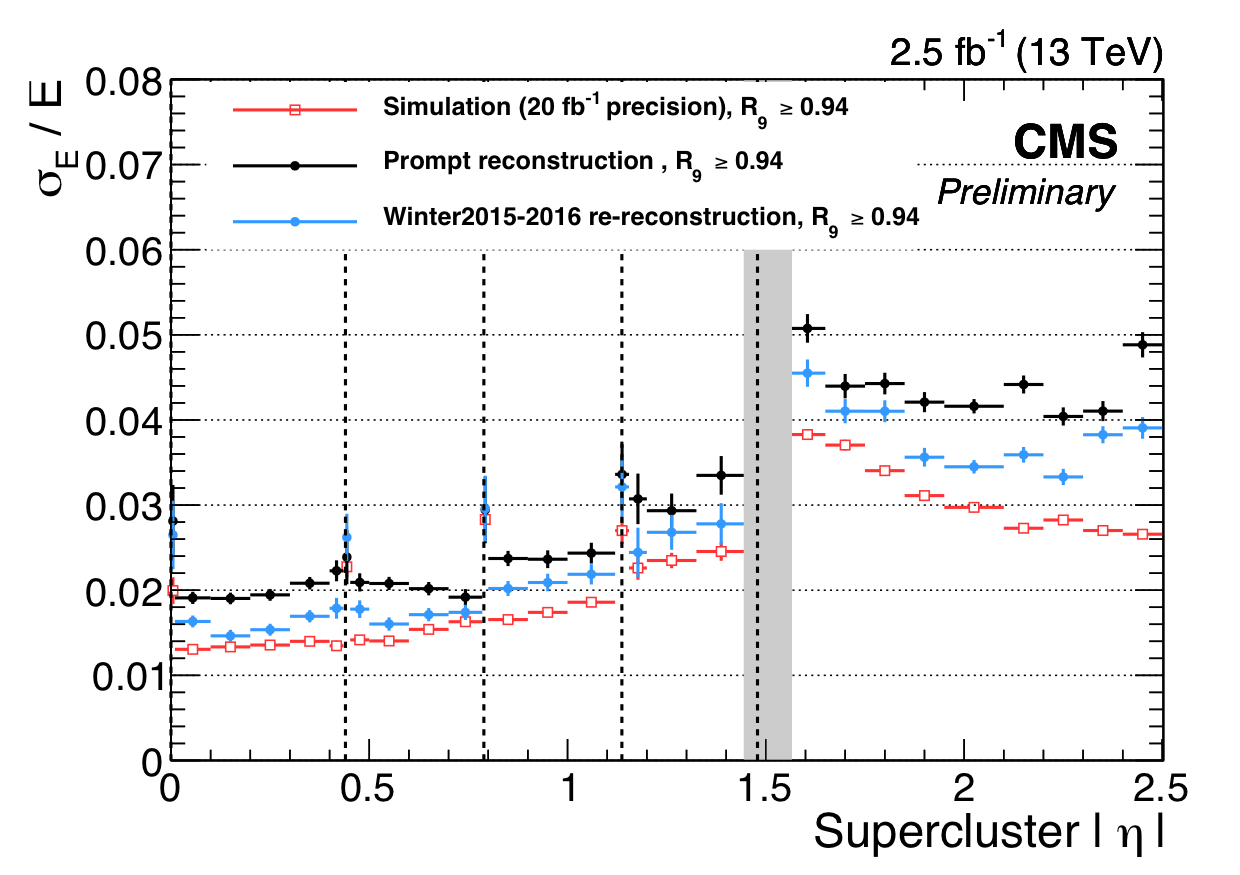
\includegraphics[width=\linewidth]{Figures/Detector/EcalEnergyResolution.png}
       \caption{Relative electron energy resolution in bins of pseudorapidity. 
       The energy resolution was calculated from an unbinned likelihood fit to $Z\rightarrow ee$ events.
        Barrel module boundaries are shown with vertical dashed lines and often correspond to regions where the resolution is somewhat degraded. The gray band at $|\eta|$ = 1.5 represents the boundary between EB and EE.
        The data correspond to 2.5\fbinv collected with the CMS detector in 2015.
        Reprinted from Reference~\cite{ECALDPGtwiki2}.}
         \label{fig:ecal_resolution}
\end{figure*}

%%%%%%%%%%%%%%%%%%%%%%%%%%%%

\section{Muon system}
\label{sec:Muon}
Aside from weakly-interacting particles such as neutrinos, muons are the only particles that make it past the HCAL. Muons do not interact via the strong force and are too heavy to be stopped by electromagnetic interactions alone. For this reason, the muon detector system is the outermost layer of CMS. Three different types of detectors are used in the muon system: drift tube (DT) chambers, cathode strip chambers (CSC), and resistive plate chambers (RPC). The muon system is located at a radial distance $r > 3.5$ m and is embedded in the return yoke for the magnetic flux.

A drift tube consists of a conducting wire held at high positive voltage in the center of a gas cell. When a charged particle passes through the gas, the gas is ionized. The freed electrons are drawn to the positively charged wire, and in turn cause more ionization as they are accelerated. The time between the passage of the initial particle and the resulting electron avalanche can be used to reconstruct the position of the interaction perpendicular to the wire.

Drift tubes are used in the barrel region of the detector and extend to $|\eta| < 1.2$. The CMS drift tubes are are made from aluminum plates and contain a mixture of 85\% Ar and 15\% CO$_2$. A gold-plated stainless steel anode wire is located at the center of each tube. The wires are held at 3.6 kV and have a thickness of 50$\mu$m. Each drift tube has dimensions 1.3 cm $\times$ 4.2 cm $\times$ 2.4 m. Four layers of drift tubes make up a superlayer, and a group of 2 or 3 superlayers makes up one muon chamber.

The endcap system uses cathode strip chambers because of their improved performance in high flux areas and non-uniform magnetic fields. Positively-charged wires are aligned perpendicular to negatively-charged wires in a gas, which gets ionized by passing muons. Electrons produce a signal in the anode wires and positive ions produce a signal in the cathode wires. This provides two position coordinates for each muon. The spatial resolution in the azimuthal direction is 150 $\mu$m. The CSCs extend the pseudorapidity coverage of the muon system to $|\eta| < 2.4$

Finally, resistive plate chambers are used in both the barrel and the endcap for more precise timing measurements. This is important for triggering purposes and to make sure each muon is assigned to the correct bunch crossing. A high voltage is applied to two large plates with a gaseous layer between them. The plates themselves have a high resistance, and the cascade caused by the passage of a muon through the gas is detected via readout strips outside the chamber. The CMS RPCs have a timing resolution of 1 ns. 

%%%%%%%%%%%%%%%%%%%%%%%%%%%%
\section{Instantaneous luminosity measurement}
\label{sec:lumi}

%https://cds.cern.ch/record/2257069?ln=en
Five different detectors (luminometers) are used to measure the instantaneous luminosity $L$ delivered by the LHC \cite{lumiPAS}: the pixel detector, the barrel drift tubes (DT), the forward hadron calorimeter (HF), and two specialized instruments, the Fast Beam Conditions Monitor (BCM1f) and the Pixel Luminosity Telescope (PLT). The last three use a fast readout system that is separate from the rest of the CMS system, and the pixel detector and DT use the standard data acquisition system. 
%cite http://cds.cern.ch/record/2257069/files/LUM-17-001-pas.pdf?version=1

Van der Meer (VdM) scans \cite{VanderMeer} are used to set an absolute calibration of each detector. Dedicated LHC running conditions allow the two beams to be scanned step-wise through one another in the two transverse directions. By finding the optimum beam position in the horizontal and vertical planes, the size of the beams at the collision point can be determined. This in turn is used to calculate the visible cross sections $\sigma_{vis}$ for each detector. The instantaneous luminosity is then given by the following, where $R$ is the measured rate for a given luminometer:
\begin{equation}
L = \frac{R}{\sigma_{vis}}
\end{equation}

The integrated luminosity $\mathcal{L}$ is the integral of all collisions taking place within CMS and represents the total amount of data collected. Figure~\ref{fig:lumi} shows the integrated luminosity delivered to CMS by the LHC and the integrated luminosity recorded by CMS during the 2016 data-taking period for 13 TeV p-p collisions. CMS collected 92.5\% of the 40.76 \fbinv delivered by the LHC. CMS can fail to record events delivered by the LHC if any sub-detector is off or misbehaving. The 2016 ``golden JSON", the full list of runs and events that are certified for use in data analysis, corresponds to 35.92 \fbinv. The total uncertainty on the integrated luminosity is 2.5\% \cite{lumiPAS}.

\begin{figure*}[h!]
	\centering
	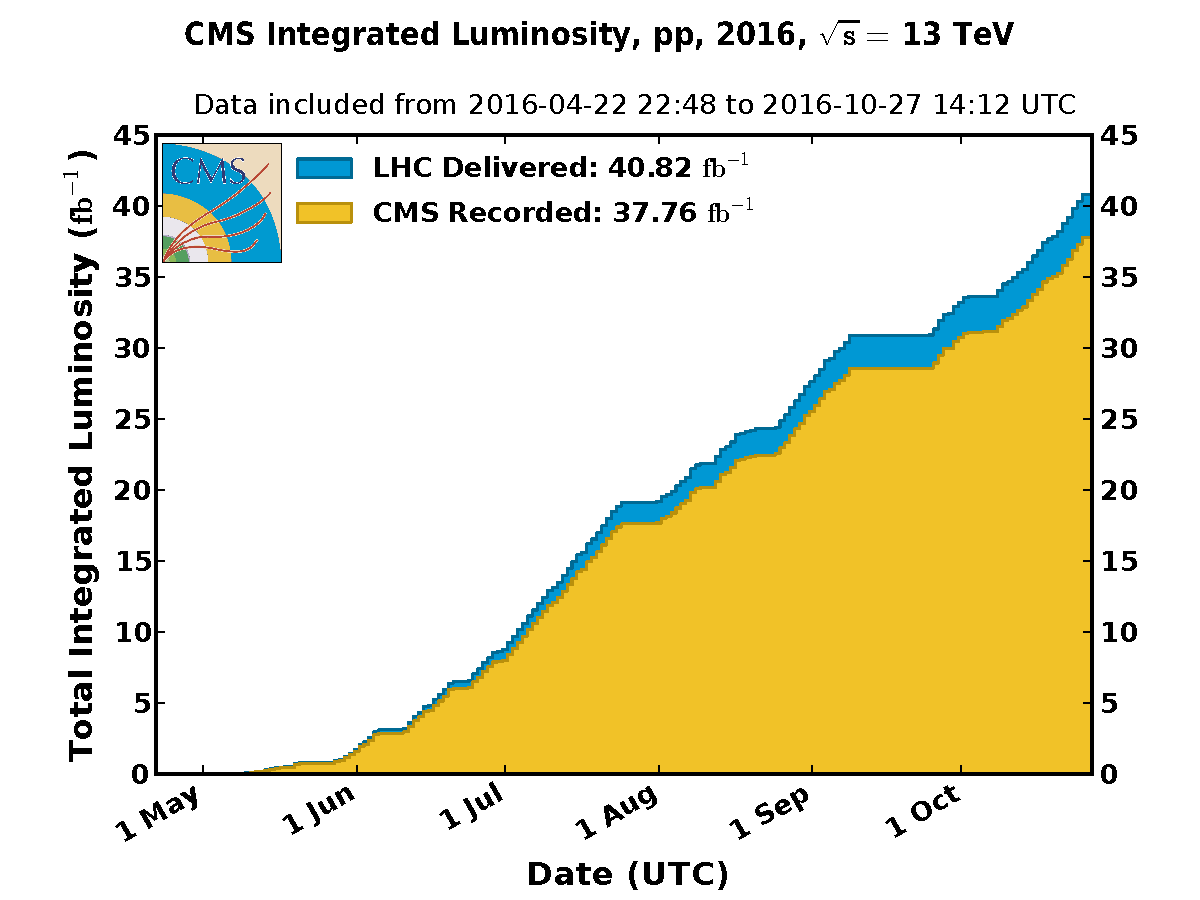
\includegraphics[width=\linewidth]{Figures/Detector/int_lumi_per_day_cumulative_pp_2016.pdf}
       \caption{Integrated luminosity delivered to CMS by the LHC (blue) and the integrated luminosity recorded by CMS (orange) during p-p collisions at $\sqrt{s}$ = 13 TeV in 2016.}
         \label{fig:lumi}
\end{figure*}







  \chapter{CMS RECONSTRUCTION}
\label{sec:EventReconstruction}

\section{Overview of the CMS reconstruction process}
\label{sec:recoOverview}

For each event that passes the trigger, the output from all of the sub-detectors described in Chapter~\ref{chap:Detector} is saved by the data acquisition system (DAQ) and eventually recorded to disk and tape. The data format at this stage is referred to as ``RAW" data. It includes information about the response of each detector, but the data are still unprocessed, aside from the minimal processing done to determine whether the event passed the trigger. ``Reconstruction" is the general term for algorithms that convert the detector response data into lists of object candidates---muons, photons, electrons, jets, etc.---and event quantities such as missing transverse momentum \ptmiss. 

Figure~\ref{fig:cmsSlice} shows how each type of particle interacts with the different layers of the CMS detector. Photons, being neutral, do not interact with the tracker, and deposit their energy in the ECAL. Electrons have a very similar response in the ECAL, but unlike photons, they also leave hits in the tracker. Hadrons deposit their energy in the HCAL, and charged hadrons have an associated track in the tracker. Finally, muons interact with the tracker and the muon system. 

 \begin{figure*}[h!]
	\centering
	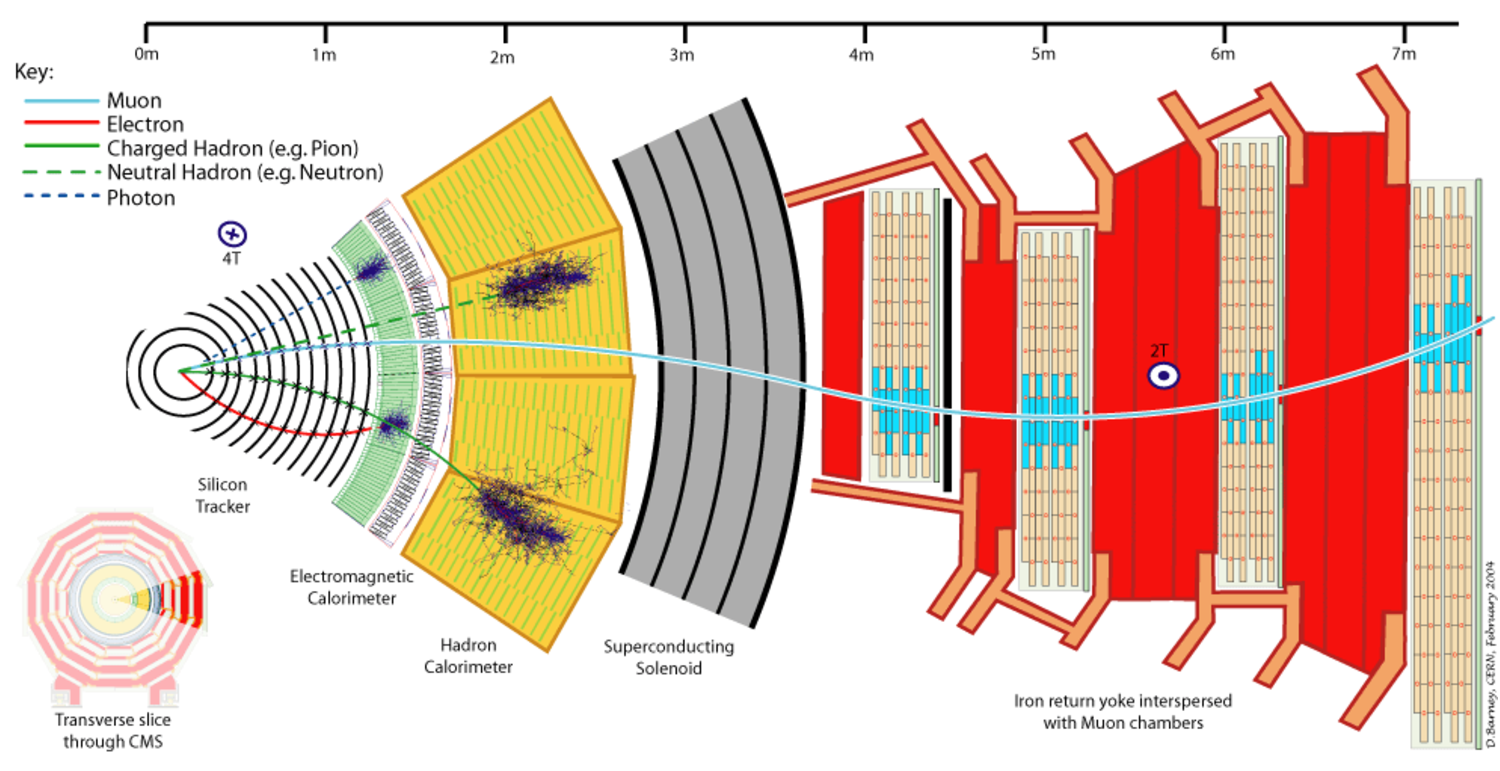
\includegraphics[width=\linewidth]{Figures/EventReconstruction/cms_slice.pdf}
       \caption{Slice of the transverse plane of the CMS detector showing how different particles interact with the detector subsystems. The most important particle for this analysis is the photon (blue dotted line), which interacts only with the ECAL (shown in green).
       Reprinted from Reference~\cite{CDS}.}
       \label{fig:cmsSlice}
\end{figure*}

Of course, the simplified picture in Figure~\ref{fig:cmsSlice} does not cover the full complexity of how particles can interact with the detector. Photons can ``convert" and produce an electron-positron pair. Hadrons can interact with the material of the tracker or ECAL, and begin to shower before reaching the HCAL. The following sections will describe in more detail how physics objects are reconstructed. 

%%%%%%%%%%%%%%%%%%%%%%%%%%%%%%%%%%%%%%%%%

\section{Particle flow algorithm}
\label{sec:ParticleFlow}
CMS uses a ``particle-flow" (PF) reconstruction algorithm \cite{ParticleFlow}. The PF approach seeks to assign each hit in the tracker and each calorimeter energy deposit (known as a cluster) to a final-state particle. This holistic view maximizes our ability to identify particles by using the full set of information provided by the detector. CMS is the first hadron accelerator experiment to use PF for reconstruction. It is made possible through the excellent spatial resolution of the tracker and calorimeters and the large bending power of the magnet. Both of these features are necessary so that signals from nearby particles do not overlap. For example, the ECAL cluster from a charged particle with $\pT =$ 20 GeV will be deviated by 5 cm from the ECAL cluster of a neutral particle emitted in the same direction, allowing the two particles to be reconstructed independently \cite{ParticleFlow}.

The ingredients to the PF algorithm are reconstructed tracks and calorimeter clusters. The relevant algorithms and methods for each of these elements will be discussed first, before describing how they are assembled to form the final lists of candidate photons, electrons, muons, and jets. 

\subsection{Track reconstruction}
\label{sec:trackReco}
Tracking in CMS takes place with a combinatorial track finder that is applied in ten iterations. The iterations use successively more complex algorithms with looser requirements on the track properties. Each iteration includes three basic steps:
\begin{itemize}
\item Seed generation: The first step is to find a track seed consisting of two or three hits compatible with a charged-particle track.
\item Track finding: Pattern recognition is used to identify hits in all layers of the tracker that are compatible with the trajectory implied by the track seed. 
\item Track fitting: A global $\chi_2$ fit is performed to determine the final properties of the track, including origin, direction, and transverse momentum. 
\end{itemize}

Because the charged particles can change direction suddenly through interactions with the tracker material, the track finder uses a Kalman filter method~\cite{Kalman}. The goal of each iteration is to find tracks with as high of a purity as possible, at the cost of moderate efficiency. The high purity is accomplished through quality cuts on the seeds and the $\chi_2$ of the track fit. Any hits that are associated with a track are masked for the subsequent iterations. This reduces the combinatorial possibilities, which in turn reduces the likelihood of random hits being built up into a fake tracks. 

In addition to particle identification and determination of transverse momentum, tracks are also used to reconstruct vertices in the event. 
The vertex with the largest value of $\Sigma\pT^2$ is identified as the primary vertex, associated with the hard-scatter interaction. The other vertices arise from soft-scatter pileup interactions. Thus, the number of reconstructed vertices in an event can be used to approximate the number of pileup interactions. Two of the later iterations of the track finder are applied with reduced constraints on the origin vertex, in order to reconstruct displaced secondary vertices from the decays of long-lived particles. 

Specialized algorithms are used to reconstruct tracks for electrons and muons. Those are described in detail next.

\subsection{Electron track reconstruction}
\label{sec:eleTrackReco}

Electrons have a higher probability of scattering in the tracker than other charged particles, and so electrons are reconstructed using a separate tracking algorithm that is optimized for multiple scatters. In particular, a Gaussian-sum filter (GSF) is used rather than a Kalman filter because it adapts better in the case of sudden and substantial momentum changes. Two approaches are used: an ECAL-driven approach and a tracker-driven approach. In the ECAL-driven method, ECAL clusters are used to infer the hit locations assuming that the cluster came from either a positron or an electron. 

The tracker-driven method is better for electrons in jets and for low-\pt electrons, when the ECAL clusters are overlapping with deposits from other particles or are too spread out to reconstruct fully. In this approach, all tracks with \pt greater than 2 GeV are used as seeds for an electron. Each track is propagated to the surface of the ECAL and checked to see if it is consistent with the position of an ECAL cluster. The final step of the algorithm uses a boosted decision tree (BDT) to quantify the goodness of fit. This last step serves to reduce the misidentification rate, which is especially important in the context of the PF algorithm to avoid double counting energy.

\subsection{Muon track reconstruction}
\label{sec:muonTrackReco}
PF muons are classified into three categories:
\begin{itemize}
\item All reconstructed tracks with $\pt > 0.5$ GeV and $|\vec{p}| > 2.5$ GeV in the inner tracker are propagated to the muon system, and classified as \textbf{tracker muons} if they match at least one hit in the muon section. 
\item \textbf{Standalone muons} are reconstructed using the muon system only. The process starts with seed tracks in the DT or CSC detectors, and a pattern recognition algorithm identifies DT, CSC, and RPC hits corresponding to the muon trajectory.
\item \textbf{Global muons} are standalone muons that are consistent with a track in the inner tracker. 
\end{itemize}

Because of the extensive amount of material that muons must traverse before reaching the muon system, the inner tracker gives the best energy resolution for muons up to 200 GeV \cite{ParticleFlow}.

\subsection{Reconstruction of calorimeter clusters}
\label{sec:clusterReco}
Calorimeter clusters are an important input for the PF algorithm. They are the sole means of detection for photons and neutral hadrons, and they are essential for improving the energy resolution of electrons and high-\pt jets. The reconstruction of a cluster begins with a seed cell (ECAL crystal or HCAL scintillating tile) that corresponds to a local energy maxima above a given threshold. Starting from the seed cell, topological clusters are formed by adding cells that share a side or corner with the cluster and have an energy that is at least twice the noise threshold. For the EB, the seed energy must be greater than 230 MeV, and subsequent crystals must have an energy of at least 80 MeV in order to be added to the topological cluster. Finally, a fit is performed to determine what fraction of the energy in the cell is associated with each PF cluster, where the number of PF clusters is equal to the number of seeds incorporated into the topological cluster.

The ECAL clusters are calibrated for photons and electrons using test beam data and radioactive sources, and residual corrections are derived using simulated single photon events. For hadrons, however, the ECAL must be re-calibrated, since the response of the ECAL to hadrons is significantly different than its response to electrons. A large simulated sample of neutral hadrons is used to derive a simultaneous calibration for the portions of the hadronic shower's energy deposited in the ECAL and HCAL. 

One complication in the reconstruction of ECAL clusters is the presence of signals known as spikes. These occur when a particle directly ionizes an ECAL APD. The result is a signal whose amplitude is $10^5$ times higher than the signal from the scintillation light alone. Because these spikes appear in only one or two crystals, they are rejected by considering the ratio of energy deposited in the central crystal to that deposited in the neighboring 4 crystals. In the case where the spike affects two adjacent crystals, the energy deposited in the two crystals is compared to that of their six neighbors. These ratios are referred to as $E_4/E_1$ and $E_6/E_2$, and are required to be less than 5\% and 10\%, respectively. 

\subsection{Particle identification}
\label{sec:partID}
A ``link" algorithm is used to connect tracks and calorimeter clusters and quantify the likelihood that two elements arose from the same particle. A dedicated procedure is used to link tracks with any ECAL clusters that are consistent with photons from electron bremsstrahlung  and to link two tracks compatible with a photon conversion. A group of linked elements is referred to as a PF block. 

Particle flow is an iterative procedure. As object candidates are identified within a PF block, their corresponding tracks and clusters are removed from further consideration. This makes PF different from more traditional reconstruction algorithms where clusters or hits could be attributed to more than one particle. The object-identification process is repeated until all tracks and clusters have been assigned to a single PF candidate. 

First, muon candidates are identified with two sets of identification criteria: one for isolated muons and one for muons inside or near jets. Next, electron candidates and photon candidates are reconstructed. Finally, any remaining tracks or calorimeter clusters in the PF block are assigned to a neutral hadron, charged hadron, or photon candidates.

%Because photons are the primary object of interest in this analysis, their reconstruction is described in more detail below. 


%%%%%%%%%%%%%%%%%%%%%%%%%%%%%%%%%%%%%%%%%

\section{Jet reconstruction}
\label{sec:Jet}
Jets are reconstructed from PF candidates using the \antikt algorithm with a distance parameter $R =$ 0.4~\cite{antikt}.  The \antikt algorithm is a sequential clustering algorithm where the distance $d_{ij}$ between two particles $i$ and $j$ and the distance $d_{iB}$ between particle $i$ and the beam $B$ are given by the following: 
\begin{equation}
\begin{aligned}
d_{ij} &= \mathrm{min}(k_{ti}^{2p},k_{ti}^{2p})\frac{\Delta^2_{ij}}{R^2} \\
d_{iB} &= k_{ti}^{2p}
\end{aligned}
\end{equation}

The value $\Delta^2_{ij}$ is equal to $(\eta_i - \eta_j)^2 + (\phi_i - \phi_j)^2$, $k_t$ is the transverse momentum of the particle, and $R$ is a distance parameter that determines the final radius of the jet.

The clustering algorithm first finds the smallest value of $d_{ij}$ and $d_{iB}$ for all particles in the event. If the minimum distance is $d_{ij}$, then particles $i$ and $j$ are combined into a single entity. If the minimum distance is $d_{iB}$, then particle $i$ is labeled a jet and removed from the list. For the \antikt algorithm, the parameter $p = -1$. Setting $p=0$ corresponds to the inclusive Cambridge/Aachen algorithm, and $p=1$ is the inclusive $k_t$ algorithm. The result of various jet-clustering algorithms is shown in Figure~\ref{fig:jetAlgorithms}. One obvious feature of the \antikt algorithm is the production of very circular jets compared to jets identified using other clustering algorithms.
 
 \begin{figure*}[h!]
	\centering
	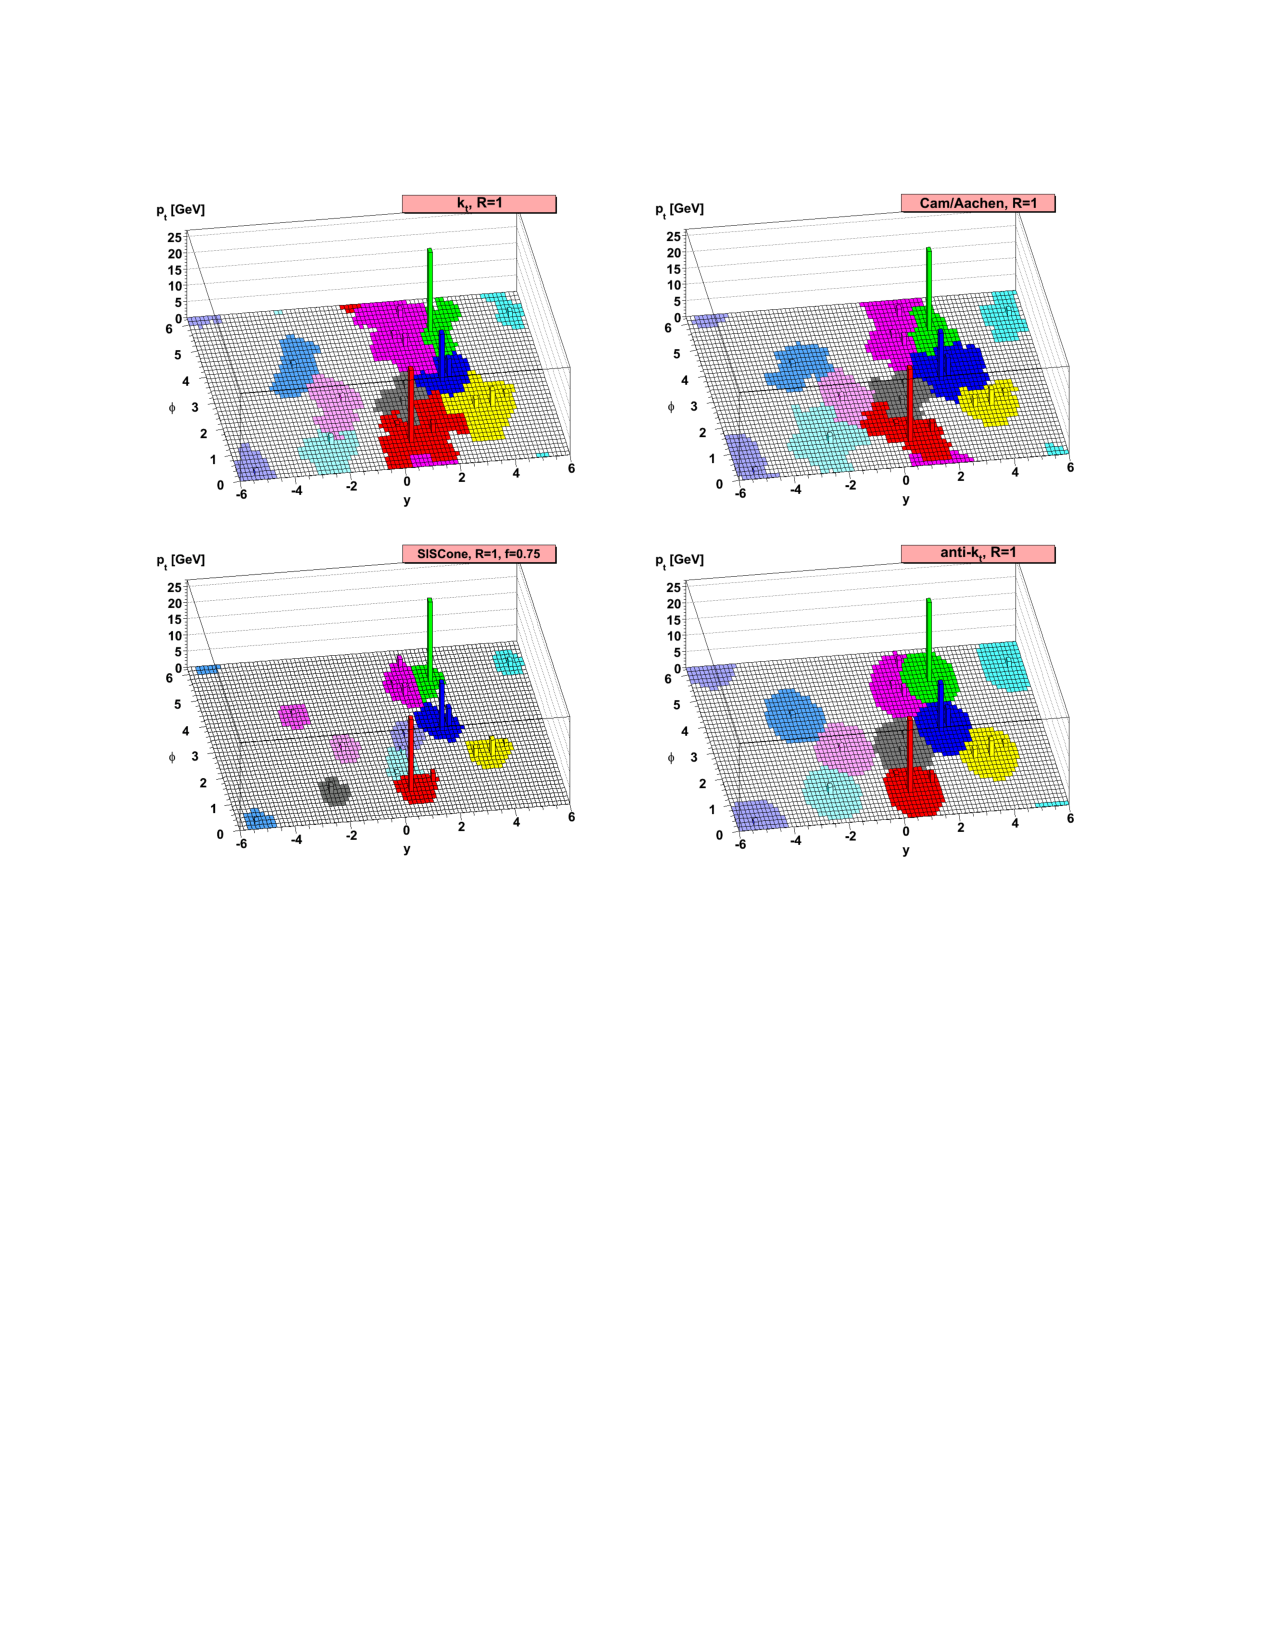
\includegraphics[width=\linewidth]{Figures/EventReconstruction/jetAlgorithms.pdf}
       \caption{Behavior of several jet-clustering algorithms illustrated with a sample parton-level event. 
       CMS uses the \antikt algorithm (bottom right) with a distance parameter $R = 0.4$.
       Reprinted from Reference~\cite{antikt}.}
       \label{fig:jetAlgorithms}
\end{figure*}
 
One benefit of the \antikt algorithm is that it is infrared and collinear (IRC) safe. Infrared safe means that \antikt jets are insensitive to nearby soft particles. In the \antikt algorithm, soft particles (those with $k_t \rightarrow 0$) have a large $d_{ij}$ and are therefore clustered last. This leaves hard jets unaffected. Soft particles could be clustered into many soft jets, but those are simple to remove during the analysis. Being infrared safe is particularly important for the high luminosity environment of the LHC, so that the clustering of the hard jets from the primary interaction is not changed by the many soft particles from pileup interactions.

Collinear safe means that very energetic initial quarks will still get reconstructed as a single jet. In the \antikt algorithm, collinear particles will have a small value of $\Delta^2_{ij}$ and will be clustered together first. Using an IRC safe algorithm is important for comparing theory and experiment, because if jets are not IRC safe, then their cross sections cannot be calculated using perturbation theory.

\subsection{Jet energy corrections}
\label{sec:JEC}

A series of jet energy corrections (JEC) are applied to the jets after clustering to improve the calibration and energy resolution \cite{JEC}. The $L1$ correction is a flat correction designed to remove contributions to the jet energy from pileup (see Section~\ref{sec:pileup} for a more thorough description of pileup mitigation techniques). The $L2$ corrections are $\eta$-dependent and the $L3$ corrections are \pt-dependent. These are calculated in simulation using generator truth information. In data, the correction factors are derived using dijet events and events where a jet is emitted back-to-back with an photon. In the latter case, the superior energy resolution of the ECAL is exploited to provide a handle on the jet energy. The effects of JEC on jet response in QCD simulation is shown in Figure~\ref{fig:JEC}.

 \begin{figure*}[h!]
	\centering
	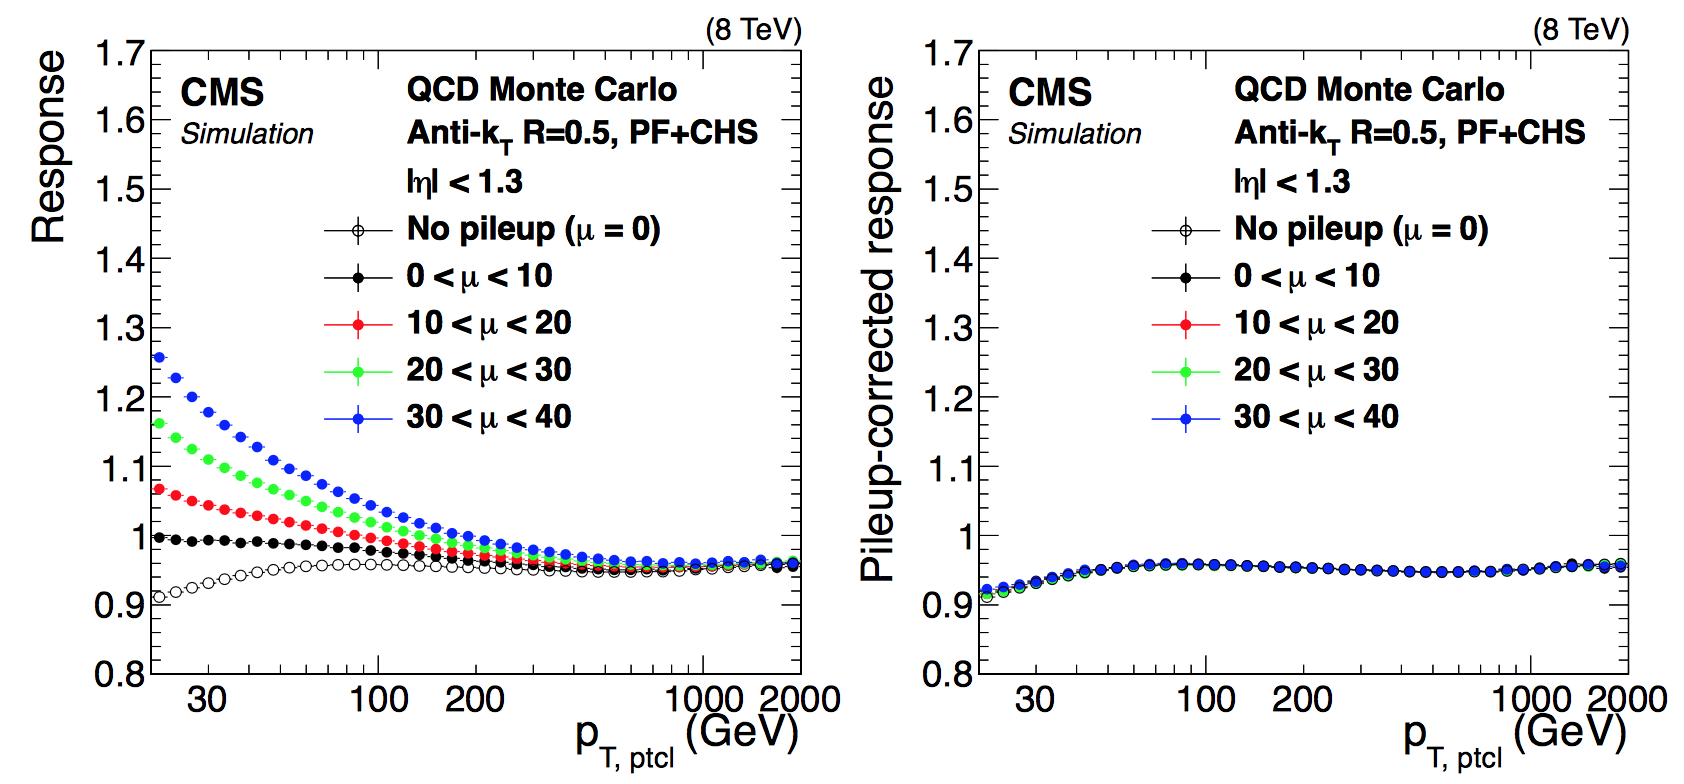
\includegraphics[width=1.0\linewidth]{Figures/EventReconstruction/JEC1.png}
	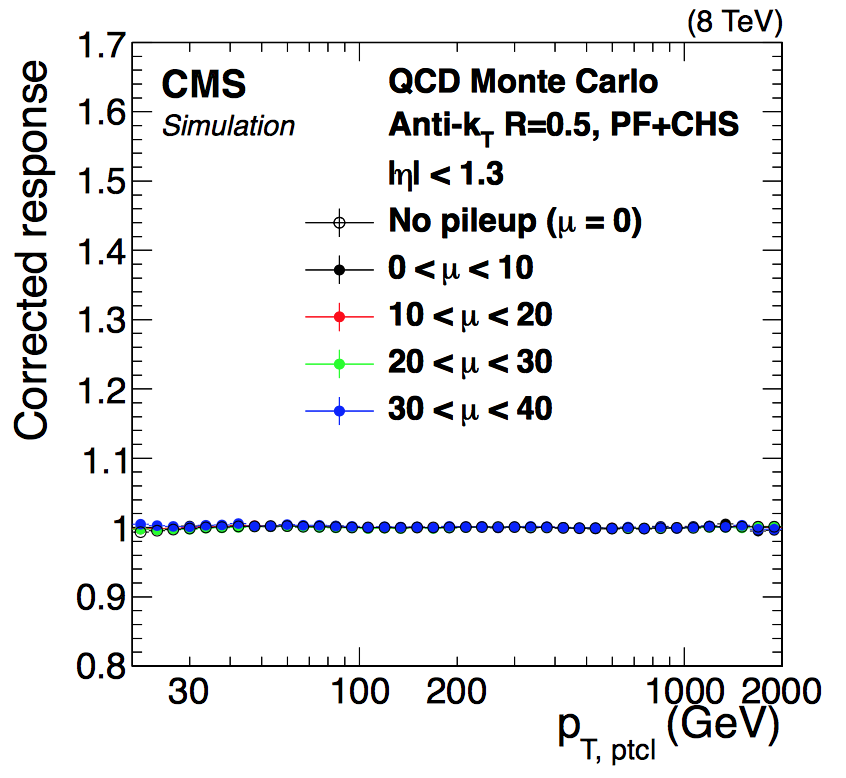
\includegraphics[width=0.5\linewidth]{Figures/EventReconstruction/JEC2.png}
       \caption{Ratio of the average reconstructed jet \pt to the particle-level jet \pt ($p_{\mathrm{T,ptcl}}$) in QCD Monte Carlo simulation.
       The ratio is calculated in bins of $p_{\mathrm{T,ptcl}}$ before applying any JEC (top left), after applying the $L1$ pileup corrections
       (top right), and after all JEC (bottom). The different curves correspond to different numbers of pileup interactions $\mu$.
       Reprinted from Reference~\cite{JEC}.}
       \label{fig:JEC}
\end{figure*}

\subsection{Jet energy resolution}
\label{sec:JER}

After the JEC are applied, resolutions of 10\% and 5\% are achieved for 100 GeV and 1 TeV jets in the barrel, respectively. Figure~\ref{fig:JER} shows the jet energy resolution as a function of jet \pt in 8 TeV simulation. 

 \begin{figure*}[h!]
	\centering
	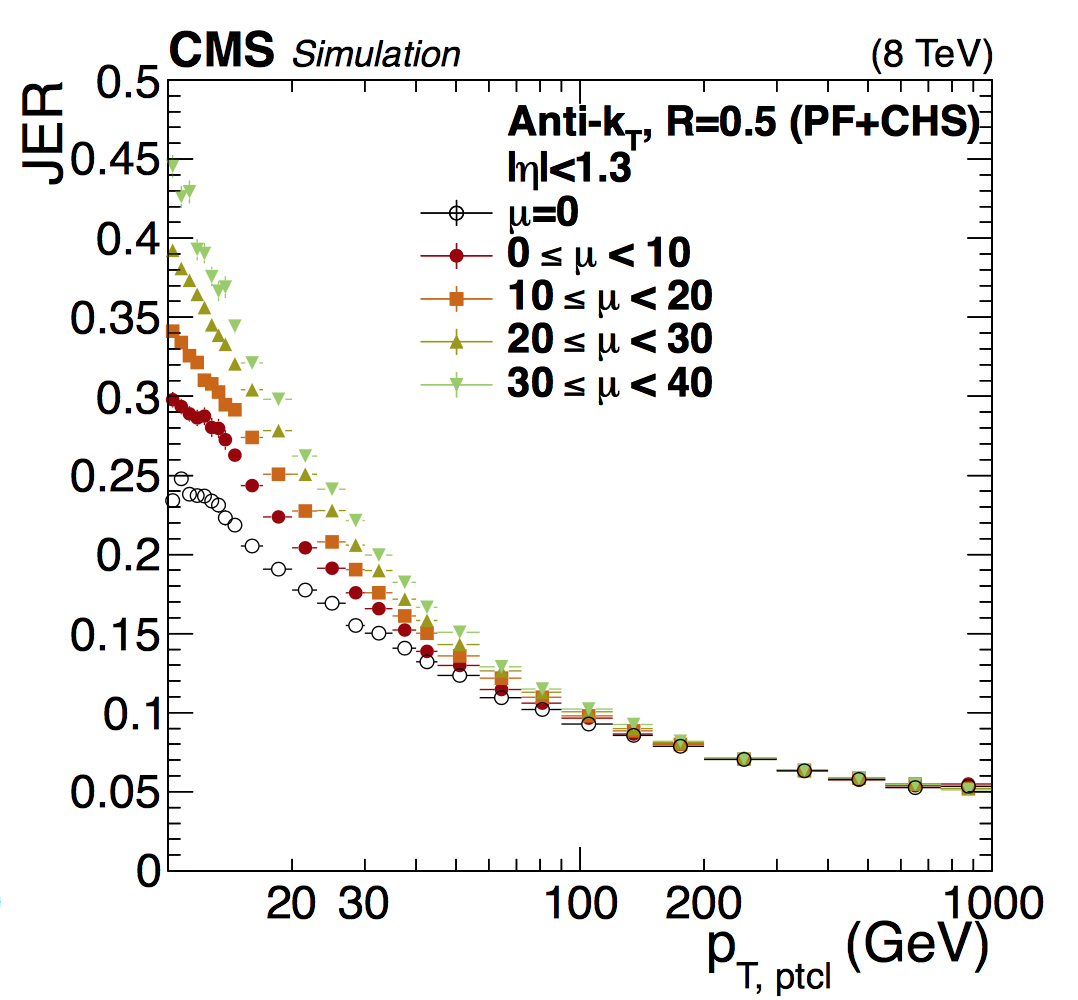
\includegraphics[width=0.65\linewidth]{Figures/EventReconstruction/JER.png}
       \caption{Jet energy resolution (JER) in 8 TeV simulation as a function of particle-level jet \pt ($p_{\mathrm{T,ptcl}}$). PF+CHS refers to particle-flow
       jets with charged hadron subtraction (see Section~\ref{sec:pileup}). Results are shown for various levels of pileup $\mu$. 
       Reprinted from Reference~\cite{JEC}.}
       \label{fig:JER}
\end{figure*}

%%%%%%%%%%%%%%%%%%%%%%%%%%%%%%%%%%%%%%%%%

\section{Missing transverse momentum}
\label{sec:MET_Reco}
After the full set of PF objects have been identified and reconstructed, the missing transverse momentum $\vec{\pt}^{\mathrm{miss}}$ is given by the following, where the sum is over all PF objects:
\begin{equation}
\vec{\pt}^{\mathrm{miss}} = \Sigma \ptvec
\end{equation}
The magnitude of this quantity is referred to as the missing transverse energy \ETmiss. For the calculation of \ETmiss in this analysis, Type-I corrections are applied, which correspond to propagating the JEC described above to the \ETmiss. 

There are several situations that can arise where particle misidentification or poor reconstruction leads to an artificially large value of \ETmiss. These are dealt with in post-processing by substituting the reconstructed particles with alternative hypotheses and checking how the \ETmiss changes. For example, very energetic charged hadrons can occasionally punch through the HCAL and leave tracks in the muon system. In this case, PF will reconstruct a neutral hadron and a muon, leading to a large value of $\vec{\pt}^{\mathrm{miss}}$ pointing in the opposite direction. If replacing the neutral hadron and muon with a charged hadron reduces the \ETmiss by 50\% or more, then that alternative reconstruction is used instead.

In addition to the post-processing corrections just described, a series of \ETmiss filters are applied. The filters are designed to tag events where the \ETmiss is poorly reconstructed. At the analysis stage, if an event fails any of the \ETmiss filters it is removed from consideration. The following \ETmiss filters applied in this analysis:
\begin{itemize}
\item Primary vertex filter
\item CSC beam halo filter
\item HBHE noise filter
\item HBHEiso noise filter
\item ECAL trigger primitive filter
\item ee badSC noise filter
\item Bad PF muon filter
\item Bad charged hadron filter
\item Duplicate muons filter
\end{itemize}

%%%%%%%%%%%%%%%%%%%%%%%%%%%%%%%%%%%%%%%%%

\section{Pileup subtraction}
\label{sec:pileup}

The presence of pileup interactions affects many aspects of the reconstruction process, in particular the jet energy resolution, lepton isolation values, and \ETmiss. Figure~\ref{fig:pileup} shows the observed pileup distribution for the 2016 CMS $p$-$p$ collisions. 

 \begin{figure*}[h!]
	\centering
	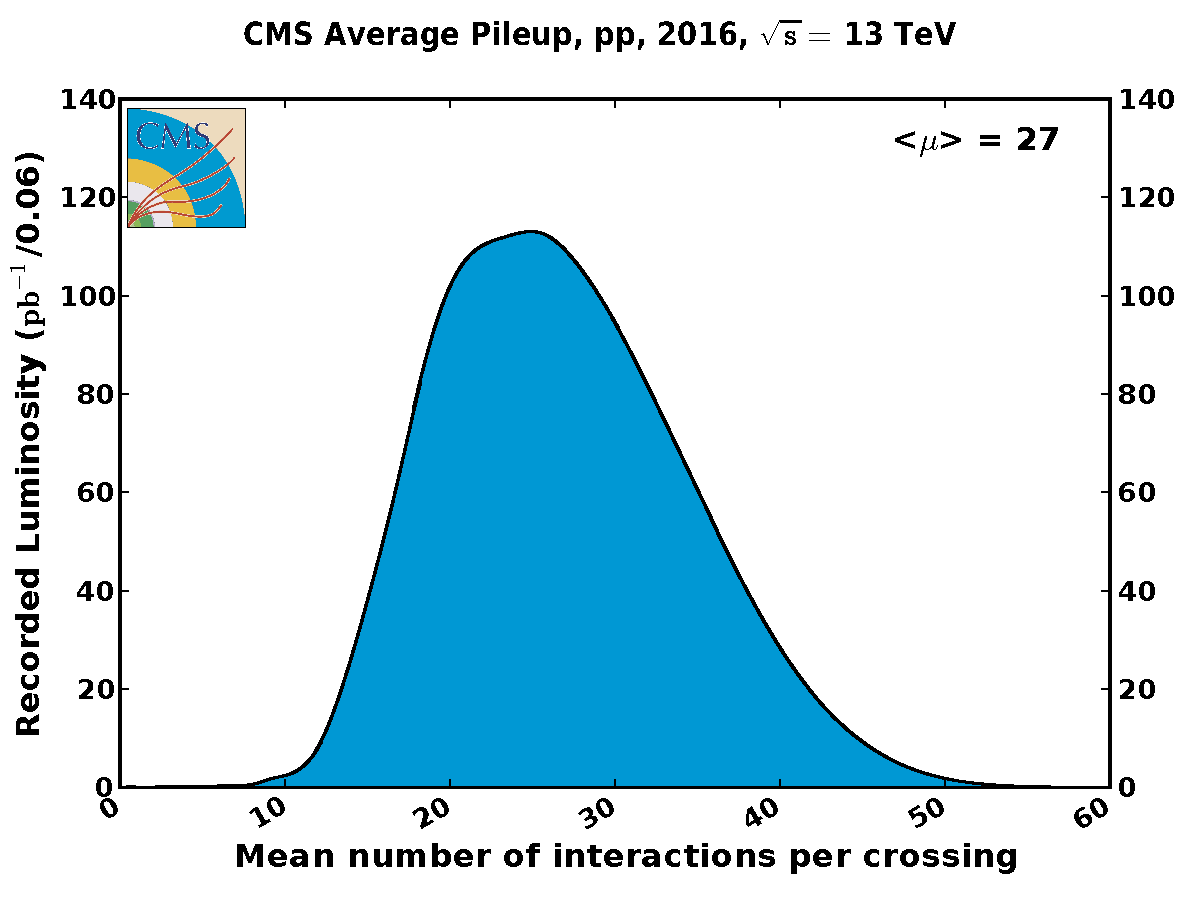
\includegraphics[width=0.65\linewidth]{Figures/EventReconstruction/pileup_pp_2016.pdf}
       \caption{Number of pileup interactions per bunch crossing as observed in $p$-$p$ collisions with the CMS detector in 2016. On average, 27 pileup interactions were observed per bunch crossing. }
       \label{fig:pileup}
\end{figure*}

Fortunately, there are several ways in which the PF algorithm can be used to mitigate the effects from pileup. Charged-hadron subtraction (CHS), for example, is the procedure of removing charged hadrons from consideration if they are associated with a pileup vertex rather than the hard-scatter vertex. Figure~\ref{fig:jetComp} shows the composition of jets in data and simulation as a function of the number of pileup interactions $\mu$. For an event with $\mu = 30$, 10\% of the uncorrected jet energy is due to charged hadrons from pileup interactions. 

 \begin{figure*}[h!]
	\centering
	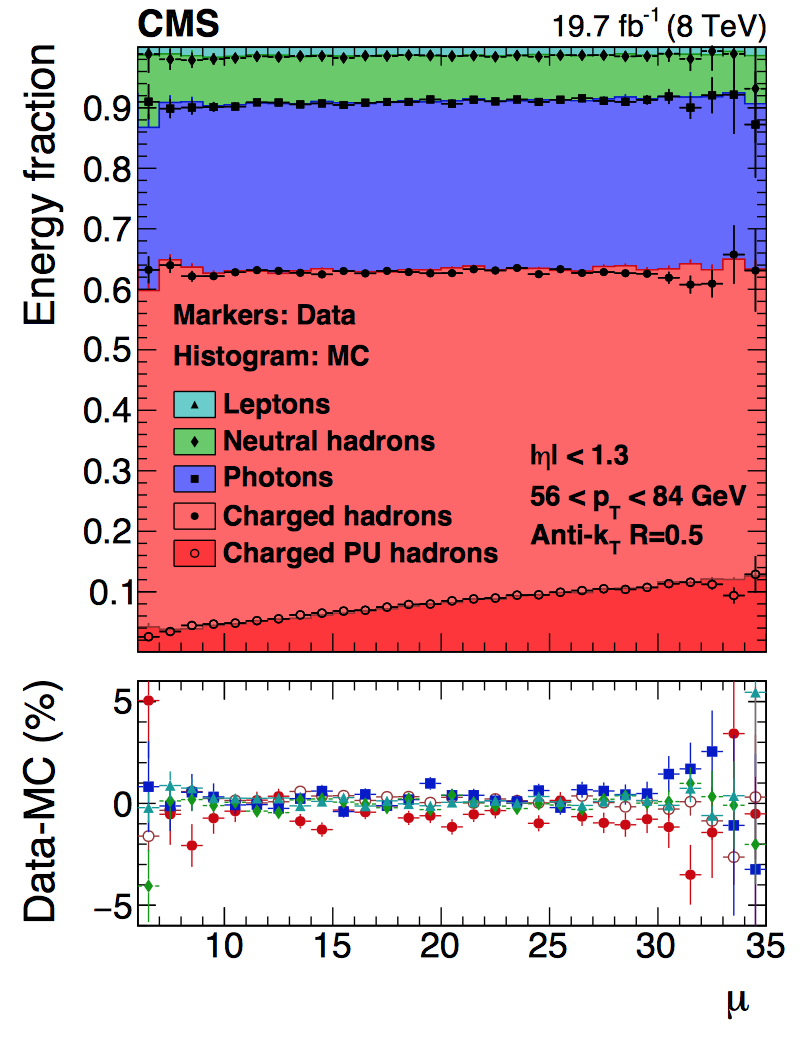
\includegraphics[width=0.8\linewidth]{Figures/EventReconstruction/jetComp.png}
       \caption{Energy composition as a function of the number of pileup (PU) interactions $\mu$ for jets in 
       data (markers) and simulation (histogram). The data distributions correspond to 19.7\fbinv collected at 
       $\sqrt{s} = 8$ TeV with the CMS detector in 2012.
       The contribution from charged hadrons from pileup is shown in dark red.
       The bottom pane shows the agreement between data and simulation for each category.
       Reprinted from Reference~\cite{ParticleFlow}.}
       \label{fig:jetComp}
\end{figure*}

The pileup contributions from photons and neutral hadrons, however, cannot be subtracted on an object-by-object basis, since there is no good way to identify whether these neutral particles were produced in the primary interaction or in a pileup interaction. These effects can only be subtracted from the event on average. 
For lepton and photon isolation, this is done by calculating $\rho$, the average \pt density due to pileup interactions. Figure~\ref{fig:rho} shows the average value of $\rho$ for events passing the primary analysis trigger. To calculate $\rho$, the \pT of all PF candidates in a fixed grid in $\eta$ and $\phi$ is summed. The value $\rho$ is defined as the median energy of the grid divided by the area in $\eta \times \phi$. 

The average contribution to the isolation sum from pileup is then given by $\rho$ times the effective area $A_{\mathrm{eff}}$ of the object under consideration. The calculation of $A_{\mathrm{eff}}$ for photons and electrons is done in a data-driven way by plotting the isolation versus $\rho$ and fitting the distribution:
\begin{equation}
I_{\mathrm{ave}}  = I_0 + A_{\mathrm{eff}}\rho
\end{equation}
where $I_0$ is an offset value and $I_{\mathrm{ave}}$ is the average isolation for a given value of $\rho$. The values for $A_{\mathrm{eff}}$ are calculated in bins of $\eta$. 

 \begin{figure*}[h!]
	\centering
	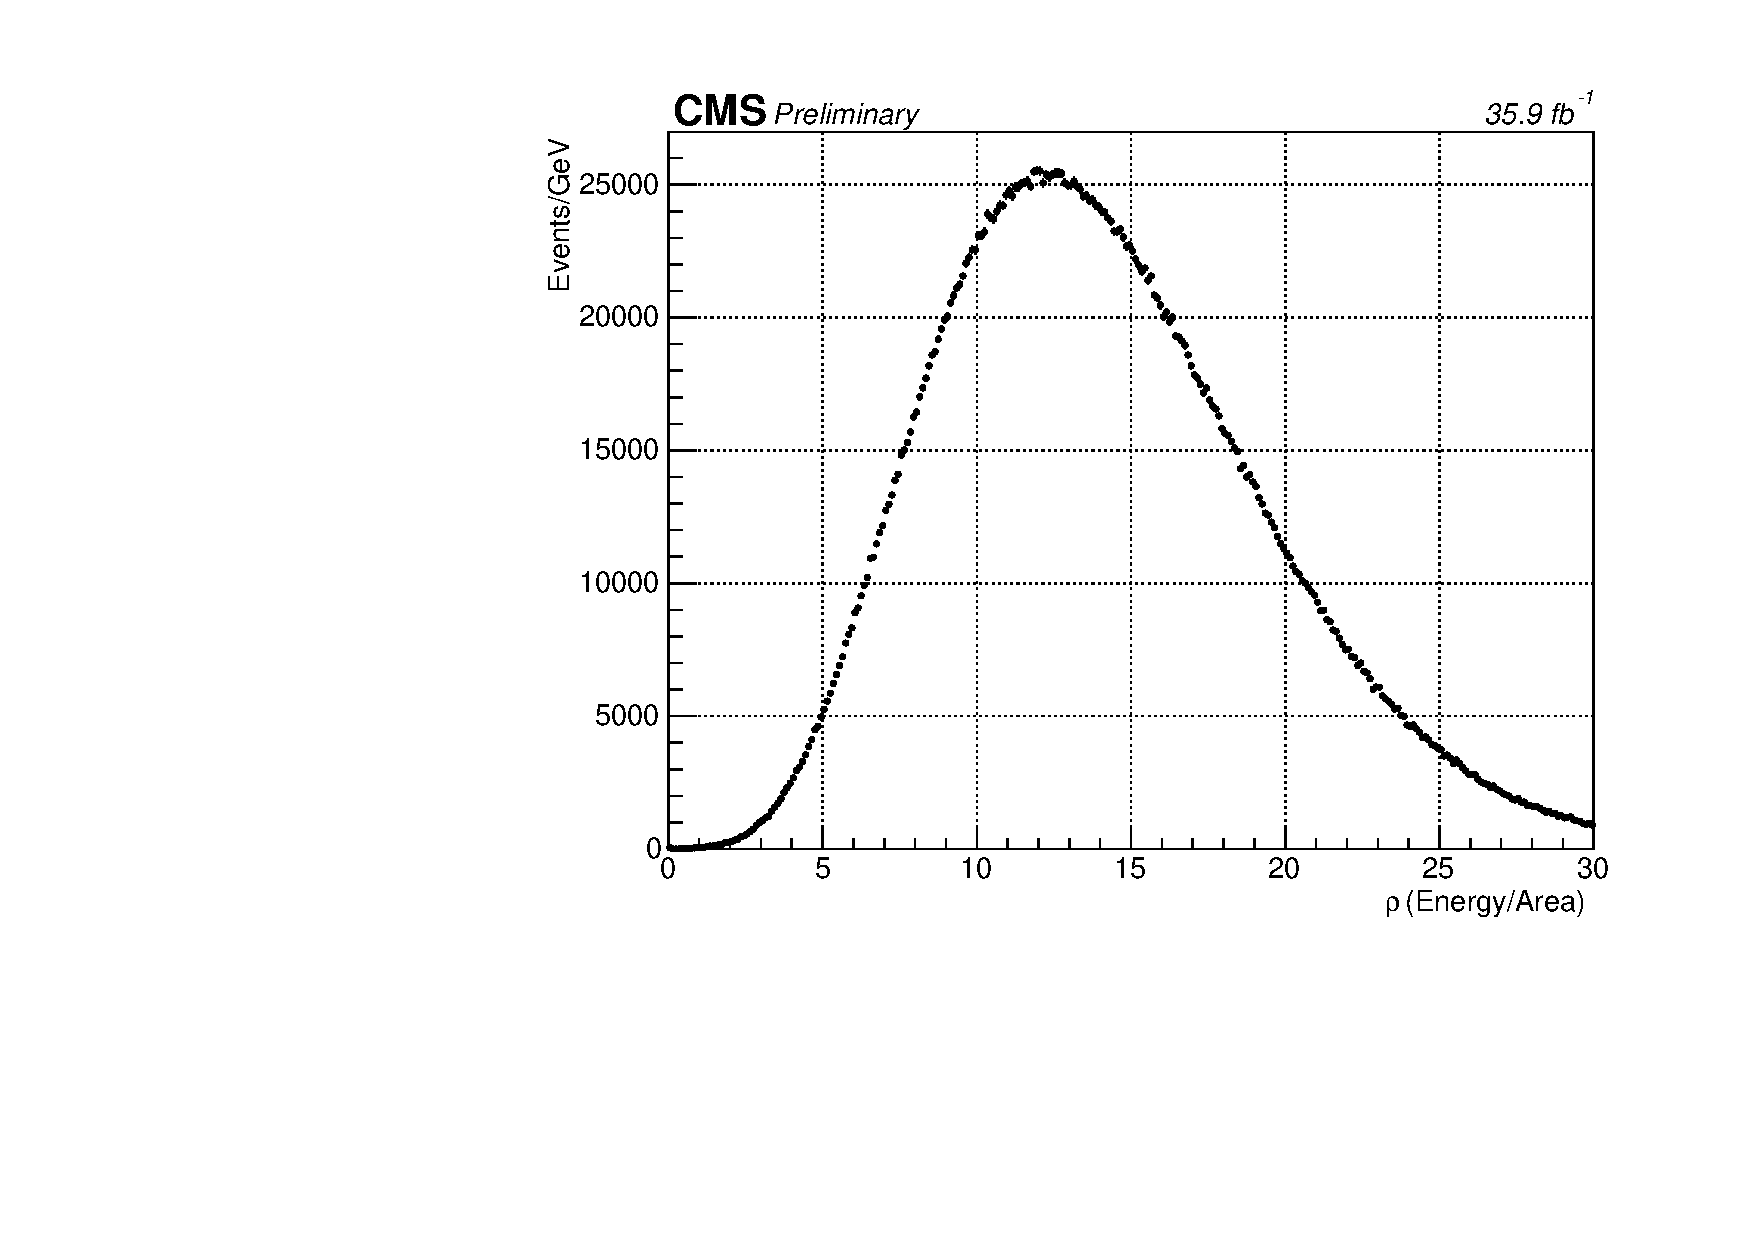
\includegraphics[width=0.8\linewidth]{Figures/EventReconstruction/rho.pdf}
       \caption{Average transverse momentum density $\rho$ for the 2016 $p$-$p$ data set. }
       \label{fig:rho}
\end{figure*}

%%%%%%%%%%%%%%%%%%%%%%%%%%%%%%%%%%%%%%%%%

\section{Photon reconstruction}
\label{sec:phoReco}
For defining jets and calculating \ETmiss, the PF reconstruction of photons and electrons is used. 
For photons and electrons used to define signal regions or control samples, however, a more optimized reconstruction that achieves a better energy resolution is employed \cite{phoPerf8TeV,elePerf8TeV}. First, an intercalibration is performed between the ECAL crystals to ensure their responses are uniform. The first-order intercalibration is applied using the laser monitoring system described in Section~\ref{sec:ECAL}. Further corrections are derived by looking at the invariant mass distribution in $\pi_0 \rightarrow \gamma\gamma$ and $\eta \rightarrow \gamma\gamma$ decays, and by noting that the energy deposited by pileup and the underlying event should be symmetric in $\phi$.

In order to achieve an excellent energy resolution, the clustering algorithm must collect the deposits corresponding to all electrons from photon conversions and all photons from electron bremsstrahlung. Similar to the PF cluster reconstruction described above, the reconstruction of photon clusters begins with a local energy maxima or ``seed" crystal. In the barrel, clusters have a fixed width of 5 crystals in $\eta$ centered on the seed. The initial cluster is made from parallel 5 $\times$ 1 strips in $\eta \times \phi$, and further strips in the $\phi$ direction (up to a total of 17 strips) are added if the energy is above a set threshold and lower than the previously added strip. In the endcap, the default cluster size is a 5 $\times$ 5 region, and adjacent 5 $\times$ 5 regions are added to the supercluster if they are sufficiently energetic. Any overlapping signal in the preshower detectors is simply added to the supercluster energy.

The variable $R_9$ is defined as the ratio of the energy in a 3 $\times$ 3 array of crystals to the energy in the full supercluster. It is used to distinguish between converted and unconverted photons. For photons that have converted, the value of $R_9$ is lower because the $e^+/e^-$ pair will separate in the $\phi$ direction due to the strong magnetic field. If $R_9$ is greater than 0.93, then the photon is classified as unconverted, and the energy of the 5 $\times$ 5 region is assigned as the photon supercluster energy. If the photon has converted (ie, $R_9 < 0.93$), then the full supercluster energy is used. 

A series of corrections are applied to the supercluster energy to account for variations in the shower containment and any potential losses for photons that convert in the tracker. Shower containment can vary for several reasons, including variations in the longitudinal depth at which the shower passes through the sides of the crystal and is lost in the inter-crystal dead space. The corrections are derived in simulation as a function of $\eta$, \ET, $R_9$, and the spread of the cluster in $\phi$. After the corrections, the photon energy resolution is better than 3\% for photons in the barrel \cite{phoPerf8TeV}.

It is worthwhile to note that the photon reconstruction algorithm does not differentiate between showers initiated by an electron and those initiated by a photon. This is important, because it means that $Z \rightarrow ee$ events can be used as a high-purity sample of $e/\gamma$ objects to study essential analysis inputs. These include the trigger efficiency (as previously described in Chapter~\ref{chap:Trigger}) and the photon ID efficiency in data and simulation (see Section~\ref{sec:phoSF}). 

Chapter~\ref{chap:EventSelect} will discuss the offline criteria used to further refine the photon selection.

  \chapter{TRIGGER SYSTEM}
\label{chap:Trigger}
%%%%%%%%%%%%%%%%%%%%%%%%%%%%%%%%%%%%%%%%%%%%%%%%%%%%%%%
%%%%%%%%%%%%%%%%%%%%%%%%%%%%%%%%%%%%%%%%%%%%%%%%%%%%%%%
%%%%%%%%%%%%%%%%%%%%%%%%%%%%%%%%%%%%%%%%%%%%%%%%%%%%%%%

\section{Overview of the CMS trigger}
\label{sec:trigOverview}
Many more collisions occur within the LHC than can be stored and analyzed. At the four interaction points of the LHC, bunches of protons collide every 25 ns. For every bunch crossing, there are on average 25 ``soft-scatter" collisions (pileup). This corresponds to an overall event rate of 1 GHz. Given that each event produces approximately 1 MB of data, it is impossible to store every event or even the majority of events. This has been especially true in recent years, with the LHC continually breaking new records for instantaneous luminosity. 

To solve this problem, the CMS detector includes a sophisticated trigger system to determine which events get written to tape and eventually analyzed. The CMS trigger  is divided into two steps: the hardware-based Level 1 (L1) trigger, and the software-based High Level Trigger (HLT). The L1 trigger reduces the rate from 1 GHz to approximately 100 kHz, and the HLT makes the final decisions necessary to reduce the rate to a few hundred Hz, the maximum amount that can be written and stored. The L1 trigger and the HLT are both highly configurable, which allows CMS to define and alter the thresholds as needed to suit different running conditions. Both steps of the CMS trigger are described in more detail below. 

%%%%%%%%%%%%%%%%%%%%%%%%%%%%%%%%%%%%%%%%%%%%%%%%%%%%%%%
%%%%%%%%%%%%%%%%%%%%%%%%%%%%%%%%%%%%%%%%%%%%%%%%%%%%%%%

\section{Level 1 trigger}
\label{sec:L1}
The L1 trigger performs rough calculations of event parameters using field-pro-grammable gate arrays located in the detector cavern. The L1 trigger only has 3.8 $\mu$s to make a decision about each event in order to reduce the output event rate to 100 kHz \cite{L1trig}. For inputs, the L1 trigger receives data from the ECAL, HCAL, and muon detector subsystems. The L1 trigger is naturally divided into two paths. The calorimeter trigger, shown schematically in Figure~\ref{fig:caloL1T}, takes data from the ECAL and HCAL subsystems and builds photon, electron, and jet candidates, as well as overall event quantities such as missing transverse momentum and total hadronic activity. The second half of the L1 trigger is the muon trigger, and its overall structure is shown in Figure~\ref{fig:muonL1T}. The output from the muon and calorimeter triggers goes into the Global Trigger (GT) processor \cite{L1_GT}, which makes the final decision regarding whether or not to accept the event. 

%%%%%%%%%%%%%%%%%%%%%%%%%%%%%%%%%%%%%%%%%%%%%%%%%%%%%%%

\subsection{Calorimeter trigger}
As shown in Figure~\ref{fig:caloL1T}, the raw inputs for the calorimeter trigger are trigger primitives (TP) from the ECAL and the HCAL. The trigger primitives from the HCAL are divided between the HCAL Barrel and Endcap (HB and HE, respectively), and the forward HCAL (HF). Trigger primitives consist of coarse information about the energy deposits  in the calorimeter for every bunch crossing. The ECAL is divided into trigger towers, groups of crystals corresponding to a region of approximately 0.087 $\times$ 0.087 in $\eta$ and $\phi$, and a TP is generated by summing the energy from each crystal in the tower. In the HCAL, TPs are generated for each trigger tower by summing the transverse energy in two consecutive time slices. 

Layer-1 of the calorimeter trigger collects the TPs from the ECAL and HCAL. Its primary role is to distribute the data to one of nine Layer-2 nodes. Each Layer-2 node receives the full set of of TPs for a particular bunch crossing, and identifies photon, electron, jet, and $\tau$-tagged jet candidates using several dynamic clustering and local maxima finding algorithms. The outputs from the Layer-2 nodes are fed into a de-multiplexing (demux) node, which ranks the candidates by transverse momentum and sends the data to the Global Trigger. 

%CITE http://iopscience.iop.org/article/10.1088/1748-0221/12/03/C03021/pdf
%CITE http://iopscience.iop.org/article/10.1088/1748-0221/11/02/C02029/pdf
%Maybe also https://arxiv.org/pdf/1609.02366.pdf

\begin{figure*}[h]
\begin{center}
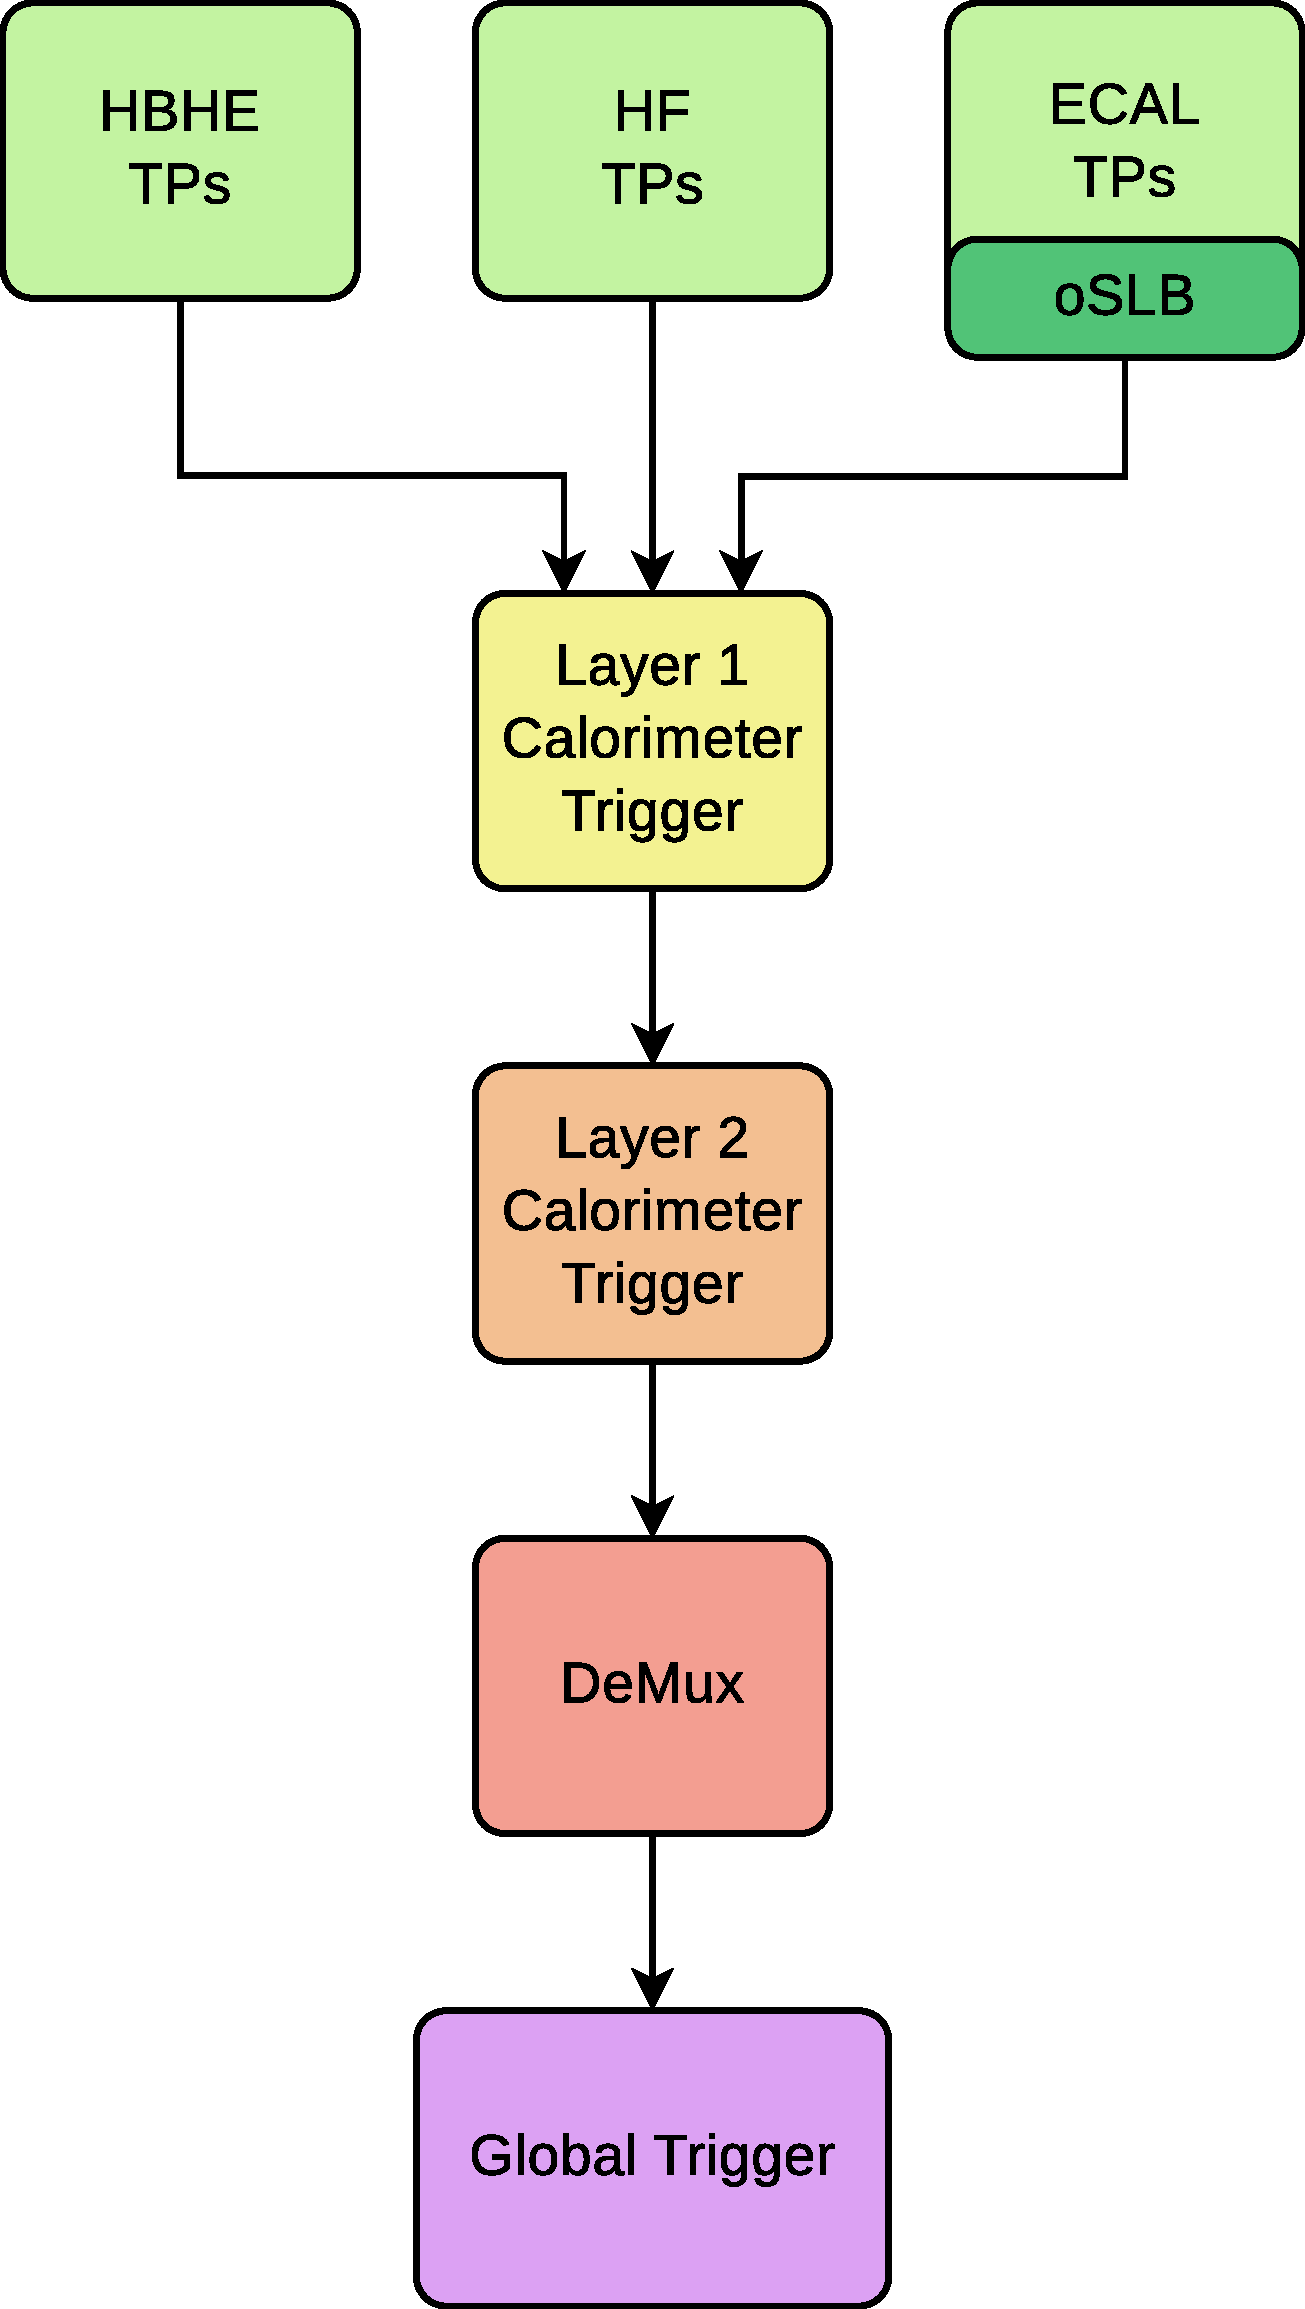
\includegraphics[width=0.6\textwidth]{Figures/Trigger/caloL1T.pdf}
\end{center}
\caption{Schematic showing the overall structure of the calorimeter half of the L1 trigger. Reprinted from Reference~\cite{L1twiki}.}
\label{fig:caloL1T}
\end{figure*}

%%%%%%%%%%%%%%%%%%%%%%%%%%%%%%%%%%%%%%%%%%%%%%%%%%%%%%%

\subsection{Muon trigger}
Information from all three of the muon detector subsystems---the cathode strip chamber (CSC) detectors, resistive plate chamber (RPC) detectors, and drift tubes (DT)---are combined in the L1 muon trigger to reconstruct muon candidates and their momenta. The muon trigger has three track-finding subsystems that reconstruct muons for different $|\eta|$ regions: the barrel track finder ($|\eta| < 0.83$), the endcap track finder ($|\eta| > 1.24$), and the overlap track finder ($0.83 < |\eta| < 1.24$).

Trigger primitives from the DT and RPC detectors are first combined in the TwinMUX system into ``super-primitives". This step serves to increase the precision of the position and timing of muon hits by taking advantage of the redundancy between the two subsystems.  The barrel track finder uses the super-primitives as inputs for its track finding algorithm, processing twelve 30$^{\circ}$ wedges in parallel. 

The endcap track finder receives information from the CSC detectors, and the overlap track finder uses information from all three subsystems. Both of these track finders use large look-up tables to convert specific hit patterns into \pT assignments for the muon candidates.

The outputs from all three track finders are sent to the Global Muon Trigger, which ranks the muons by quality and transverse momentum and sends the top 8 muon candidates to the Global Trigger for a final decision on the event.

\begin{figure*}[h]
\begin{center}
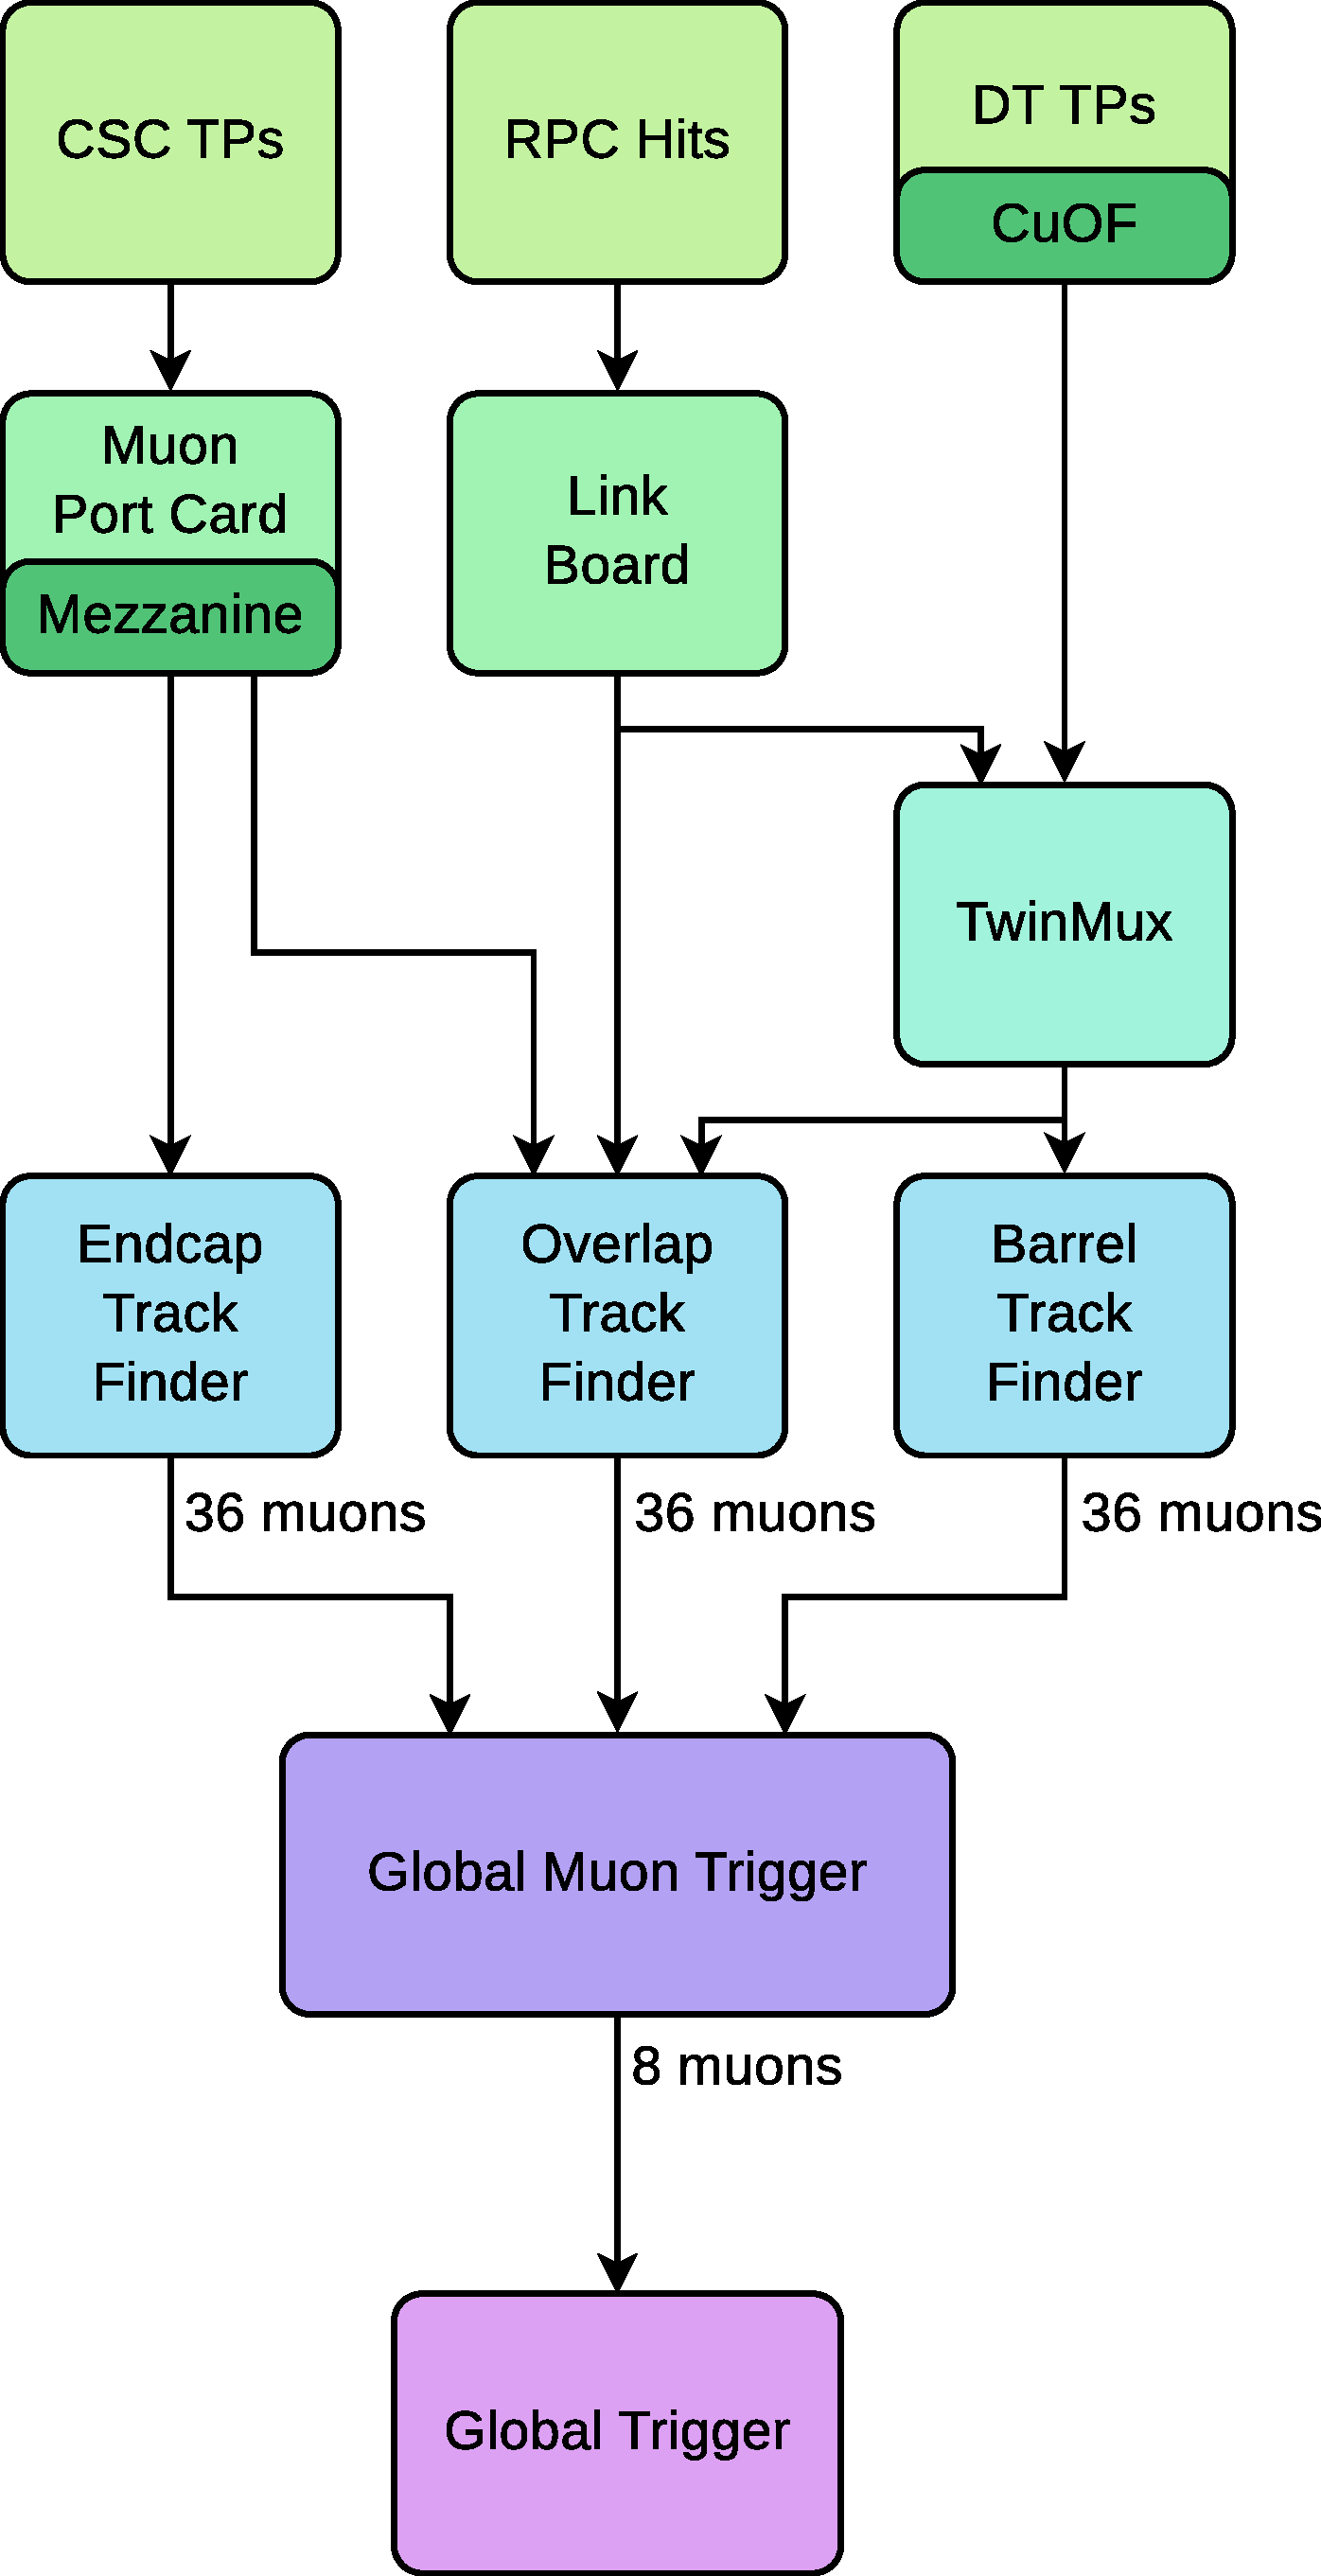
\includegraphics[width=0.7\textwidth]{Figures/Trigger/muonL1T.pdf}
\end{center}
\caption{Schematic showing the overall structure of the muon half of the L1 trigger. Reprinted from Reference~\cite{L1twiki}.}
\label{fig:muonL1T}
\end{figure*}

\subsection{Global Trigger}
The reconstructed objects and quantities built by the calorimeter trigger and the muon trigger---photon, electron, jet, and muon candidates, missing energy and total hadronic activity---get sent to the Global Trigger (GT) for final processing. The GT can implement up to 512 different trigger algorithms using these objects \cite{L1_GT}. For example, one of the L1 algorithms (or ``seeds") used in this analysis is DoubleEG\_22\_12.  This path requires two electron or photon candidates with leading and trailing \pT greater than 22 and 12 GeV, respectively.

A full set of L1 algorithms is known as the L1 menu. The menu can be adjusted as needed to meet the requirements of the CMS physics program. 
In particular, the ``prescale" of each L1 seed can be adjusted 
to take full advantage of varying LHC running conditions and instantaneous luminosities. 
A prescale is an integer value $N$ used to reduce the rate of a trigger path by only applying the trigger to
1 out of every $N$ events. For the 2016 data-taking period, the lowest unprescaled DoubleEG seed was
DoubleEG\_22\_12, but the menu also included several prescaled algorithms with lower \pT thresholds.

%%%%%%%%%%%%%%%%%%%%%%%%%%%%%%%%%%%%%%%%%%%%%%%%%%%%%%%
%%%%%%%%%%%%%%%%%%%%%%%%%%%%%%%%%%%%%%%%%%%%%%%%%%%%%%%

\section{High Level Trigger}
\label{HLT}
The High Level Trigger (HLT) uses a large farm of commercially available PCs to further reduce the rate to a few hundred Hz. The HLT receives fully-built event data from the CMS data acquisition system (DAQ) and processes only those bunch crossings that have passed the L1 trigger. The 13,000 CPU cores used in the HLT run the CMS software framework referred to as CMSSW, the same framework that is used in the offline analysis. 

Approximately 400 HLT ``paths" are used to select events of interest. Each HLT path is a single set of criteria for accepting an event if it satisfies a particular physics signature. The full list of HLT paths is referred to as the HLT menu. The HLT menu is often updated to reflect improvements in the software, updates to the calibrations, changes to the beam condition, or revisions to the physics signatures being sought. 

The HLT has a limited amount of time it can spend making a decision on a single bunch crossing. For this reason, each HLT path is ``seeded" by one or more L1 algorithms. When an event gets passed to the HLT from the DAQ, the HLT only processes those paths that are seeded by L1 bits that fired. 
For example, the diphoton HLT path used in this analysis is seeded by a combination of single and double e/$\gamma$ (EG) L1 algorithms. If none of those particular L1 seeds fired, then the HLT path will not get run on that event. 

In addition, significant time is saved at the HLT by running the steps (filters) of each HLT path in order from least CPU intensive to most CPU intensive. If the event fails any of the filters in an HLT path, then the processing is immediately aborted and the remaining filters do not get run. In the diphoton HLT path described below, the most CPU intensive filter is the invariant mass calculation, and therefore it runs only if the event has already satisfied the rest of the path's requirements.

Based on its general physics signature, each HLT path is assigned to a primary data set (PD). For this analysis, signal events are included in the DoubleEG PD. The SingleElectron and SinglePhoton data sets are also used for object identification studies.

%%%%%%%%%%%%%%%%%%%%%%%%%%%%%%%%%%%%%%%%%%%%%%%%%%%%%%%
%%%%%%%%%%%%%%%%%%%%%%%%%%%%%%%%%%%%%%%%%%%%%%%%%%%%%%%
%%%%%%%%%%%%%%%%%%%%%%%%%%%%%%%%%%%%%%%%%%%%%%%%%%%%%%%

\section{Analysis triggers}
\label{sec:analysisTrig}

The HLT paths used in this analysis are listed in Table~\ref{tab:triggers}. These triggers were developed for the $H \rightarrow \gamma\gamma$ search, 
but also serve our analysis well. Two triggers are used: a primary trigger that requires the diphoton invariant mass to be greater than 90 GeV, and a control
trigger that was designed to collect $Z\rightarrow ee$ events. 

\begin{table}[ht]
\caption{HLT TRIGGER PATHS}
\label{tab:triggers}
\begin{center}
\begin{tabular}{|c|}
\hline
\hline
\bf{Primary Trigger}   \\                                                                                                 
HLT\_Diphoton30\_18\_R9Id\_OR\_IsoCaloId\_AND\_HE\_R9Id\_Mass90\_v* \\     
\hline                                               
\bf{Control Sample Trigger} \\                                                                                       
HLT\_Diphoton30\_18\_R9Id\_OR\_IsoCaloId\_AND\_HE\_R9Id\_ \\
DoublePixelSeedMatch\_Mass70\_v* \\                              
\hline
\hline
\end{tabular}
 \justify{List of triggers used to accumulate the events in the 35.9~\fbinv data sample.}
\end{center}
\end{table}

\subsection{Trigger requirements}
\label{sec:trigRequirements}
The requirements to pass the various parts of the trigger
are listed in Table~\ref{tab:trigcuts}.
Because we only use photons with $|\eta| < 1.4442$ in this analysis
(see Chapter~\ref{chap:EventSelect} for full event selection requirements), we list only
the trigger requirements in the barrel. 

\begin{table}[ht]
\caption{PRIMARY TRIGGER REQUIREMENTS}
\label{tab:trigcuts}
\begin{center}
\begin{tabular}{|c| c |}
\hline
\hline
\textbf{Name} & \textbf{Cuts} \\
\hline
Diphoton30\_18\_ &  Leading photon \pt$ > 30$ GeV \\
 & Sub-leading photon \pt$ > 18$ GeV \\
 \hline
R9Id\_ & $R_9 > 0.85$\\
\hline
IsoCaloId\_ &  \sigmaietaieta$< 0.015$\\
 & ECAL isolation~$<~(6 + 0.012 \times$Photon \ET) \\
 & Track isolation~$<~(6 + 0.002 \times$Photon \ET) \\
 \hline
HE\_R9Id\_ & H/E $< 0.1$ \\
 & $R_9 > 0.5$\\
 \hline
Mass90\_  & $m_{\gamma\gamma} > 90$ GeV \\                                                                        
\hline
\hline
\end{tabular}
 \justify{Definition of cuts used in the primary analysis trigger, HLT\_Diphoton30\_18\_ R9Id\_OR\_IsoCaloId\_AND\_HE\_R9Id\_Mass90\_v*}
\end{center}
\end{table}

Each of the variables used in the trigger are defined below. See Chapter~\ref{chap:EventSelect} for more information on how energy deposits in the calorimeter are reconstructed into photon ``superclusters".

\begin{itemize}
\item{\ET:} The transverse energy \ET of a photon is defined
as the magnitude of the projection
of the photon momentum on the plane perpendicular to the beam axis.
\item{$R_9$:} The variable $R_9$ is
a measure of the overall transverse spread of the shower. It is the ratio
of the energy deposited in the ECAL inside a 3x3 crystal matrix centered on
the most energetic crystal in the supercluster to the supercluster
 raw energy.
\item{$\sigma_{i\eta i \eta}:$} The shower width \sigmaietaieta is
      the log-fractional energy-weighted spread within the 5x5 crystal matrix centered on the
      crystal with the largest energy deposit in the supercluster. The symbol
      i$\eta$ indicates that the variable is obtained by measuring position by
      counting crystals.
\item{ECAL isolation:} The ECAL isolation is
      the sum of all energy deposits in the ECAL within a cone of \dR
      $<$0.3 centered on the photon.
\item{Track isolation:} The track isolation is
      the sum of the energies of tracks in the tracker within a cone of \dR
      $<$0.3 centered on the photon.
\item{H/E:} The ratio between the energy deposited in the HCAL
      tower closest to the supercluster position and the energy deposited to
      that supercluster in the ECAL is referred to as H/E.
  \end{itemize}

All photons are required to pass the H/E and loose $R_9$ cuts in
\_HE\_R9Id\_, and either the tighter $R_9$ cuts in
\_R9Id\_ or the isolation and shape cuts in \_IsoCaloId\_.
The leading leg of the filter requires the photon candidate
to be matched to an L1 seed. It can be matched to one of several
SingleEG and DoubleEG L1 filters, but the largest contribution comes
from the lowest unprescaled triggers: namely, SingleEG40 and
DoubleEG$\_$22$\_$15.
Both photons must satisfy the trailing filter, which is unseeded.
In addition to the cuts listed above, the invariant mass of
the diphoton system is required to be greater than 90 GeV.

The control trigger shares all of the same requirements as the primary trigger, with two exceptions: 
the invariant mass of the two electromagnetic objects is required to be greater than 55 GeV rather than 90 GeV, 
and both electromagnetic objects are required to be matched to a pixel seed. A pixel seed is defined
as at least two hits in the pixel detectors that are consistent with the location of the energy deposit in the ECAL. 

%%%%%%%%%%%%%%%%%%%%%%%%%%%%%%%%%%%%%%%%%%%%%%%%%%%%%%%
%%%%%%%%%%%%%%%%%%%%%%%%%%%%%%%%%%%%%%%%%%%%%%%%%%%%%%%
%%%%%%%%%%%%%%%%%%%%%%%%%%%%%%%%%%%%%%%%%%%%%%%%%%%%%%%

\section{Trigger efficiency}
\label{sec:trigEff}
An important input to the analysis is the overall trigger efficiency. Due to the similarity of the ECAL response 
to electrons and photons, the trigger efficiency can be calculated from 
$Z\rightarrow ee$ events in data using the tag-and-probe method. In this method, two electron candidates
are required. One serves as the ``tag" and is required to pass loose photon identification criteria. 
The second electron candidate serves
as the ``probe" and has to satisfy the same selection criteria as our offline photon identification (see Section~\ref{sec:ObjSelect}). 
In order to ensure a high purity of electromagnetic objects, the invariant mass of the di-electron system must be between 75 and 105~GeV. 
For this study, tag-and-probe events were collected by requiring that the tag pass
a single electron control trigger, HLT\_Ele27\_WPTight\_Gsf.


The efficiency $\epsilon$ of the HLT path or trigger filter that is being studied is given by the following equation, where $N_{total}$ is the total number of tag and probe pairs 
passing all requirements, and $N_{pass}$ is the number of tag and probe pairs in which  the probe passes the trigger filter.
\begin{equation}
 \epsilon_{trig} = N_{pass} / N_{total}
\end{equation}

\subsection{Efficiency of primary trigger}
\label{sec:TnP_Eff}

Because our analysis trigger is seeded by the OR of multiple SingleEG and DoubleEG L1 seeds, the names of which changed over the course of the 2016 data-taking period, calculating the L1 efficiency on its own proved to be tricky. Instead, it was simpler to calculate the total efficiency with which photon candidates pass both the L1 seed and the leading leg of the HLT path. This efficiency as a function of photon \pt is shown in Figure~\ref{fig:leadEff}. The efficiency was fit to an error function to calculate the overall efficiency at the plateau. For photon \pt $>~40$ GeV, the leading filter is 98.2\% efficient.

\begin{figure*}[h]
\begin{center}
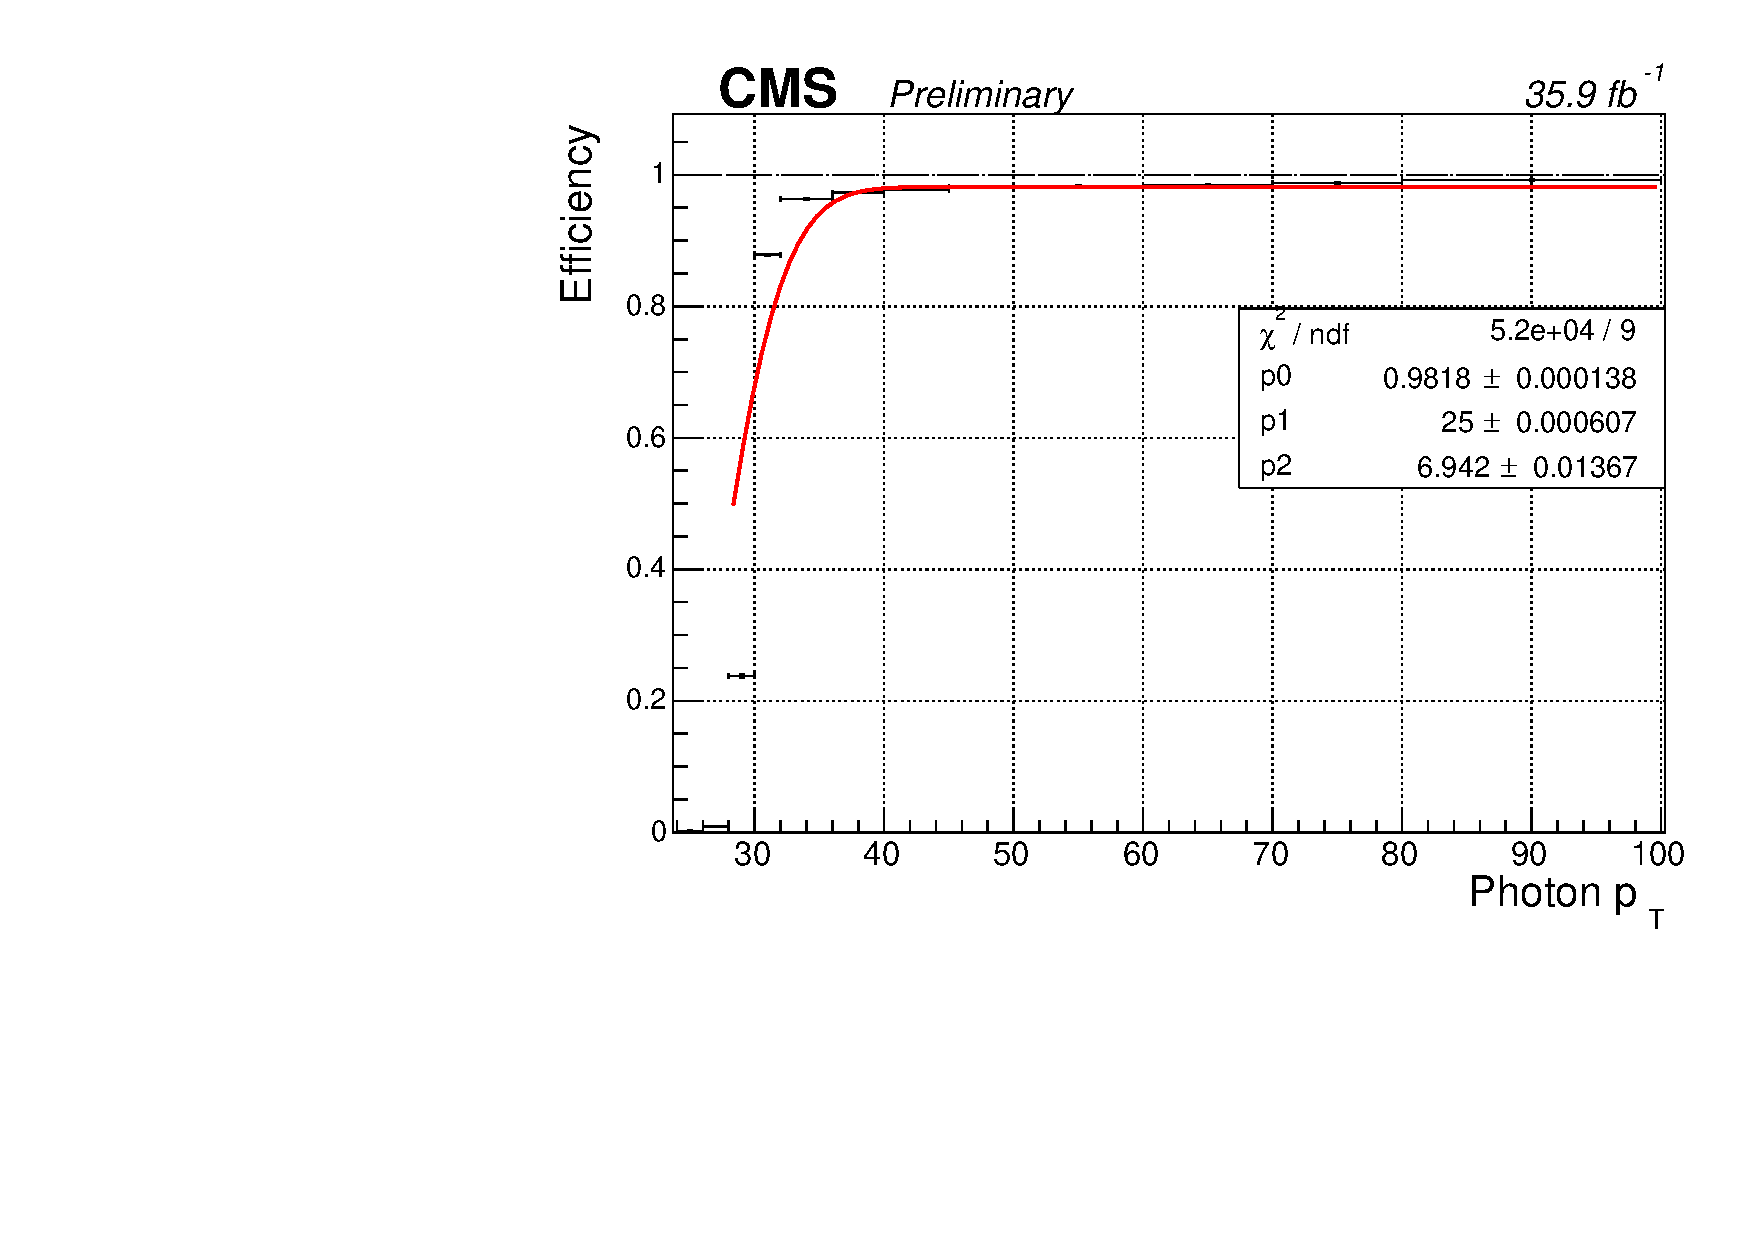
\includegraphics[width=0.9\textwidth]{Figures/Trigger/leadingEff.pdf}
\end{center}
\caption{Efficiency of the L1 seed and the leading leg of the primary analysis trigger with respect to photon \pT. 
For $\pT > 40$ GeV, the trigger is 98.2\% efficient.}
\label{fig:leadEff}
\end{figure*}

Tag and probe objects for the trailing leg efficiency must pass the same set of requirements as those used in the leading leg efficiency calculation, with the additional requirement that the tag must pass the leading filter. This requirement arises from the way HLT modules are structured. Filters are processed sequentially, and if an event fails one filter, the subsequent filters are skipped. Figure~\ref{fig:trailEff} shows the efficiency of the trailing filter as a function of photon \pt. For $\pT > 40$ GeV, the trigger is 99.8\% efficient.

\begin{figure*}[h]
\begin{center}
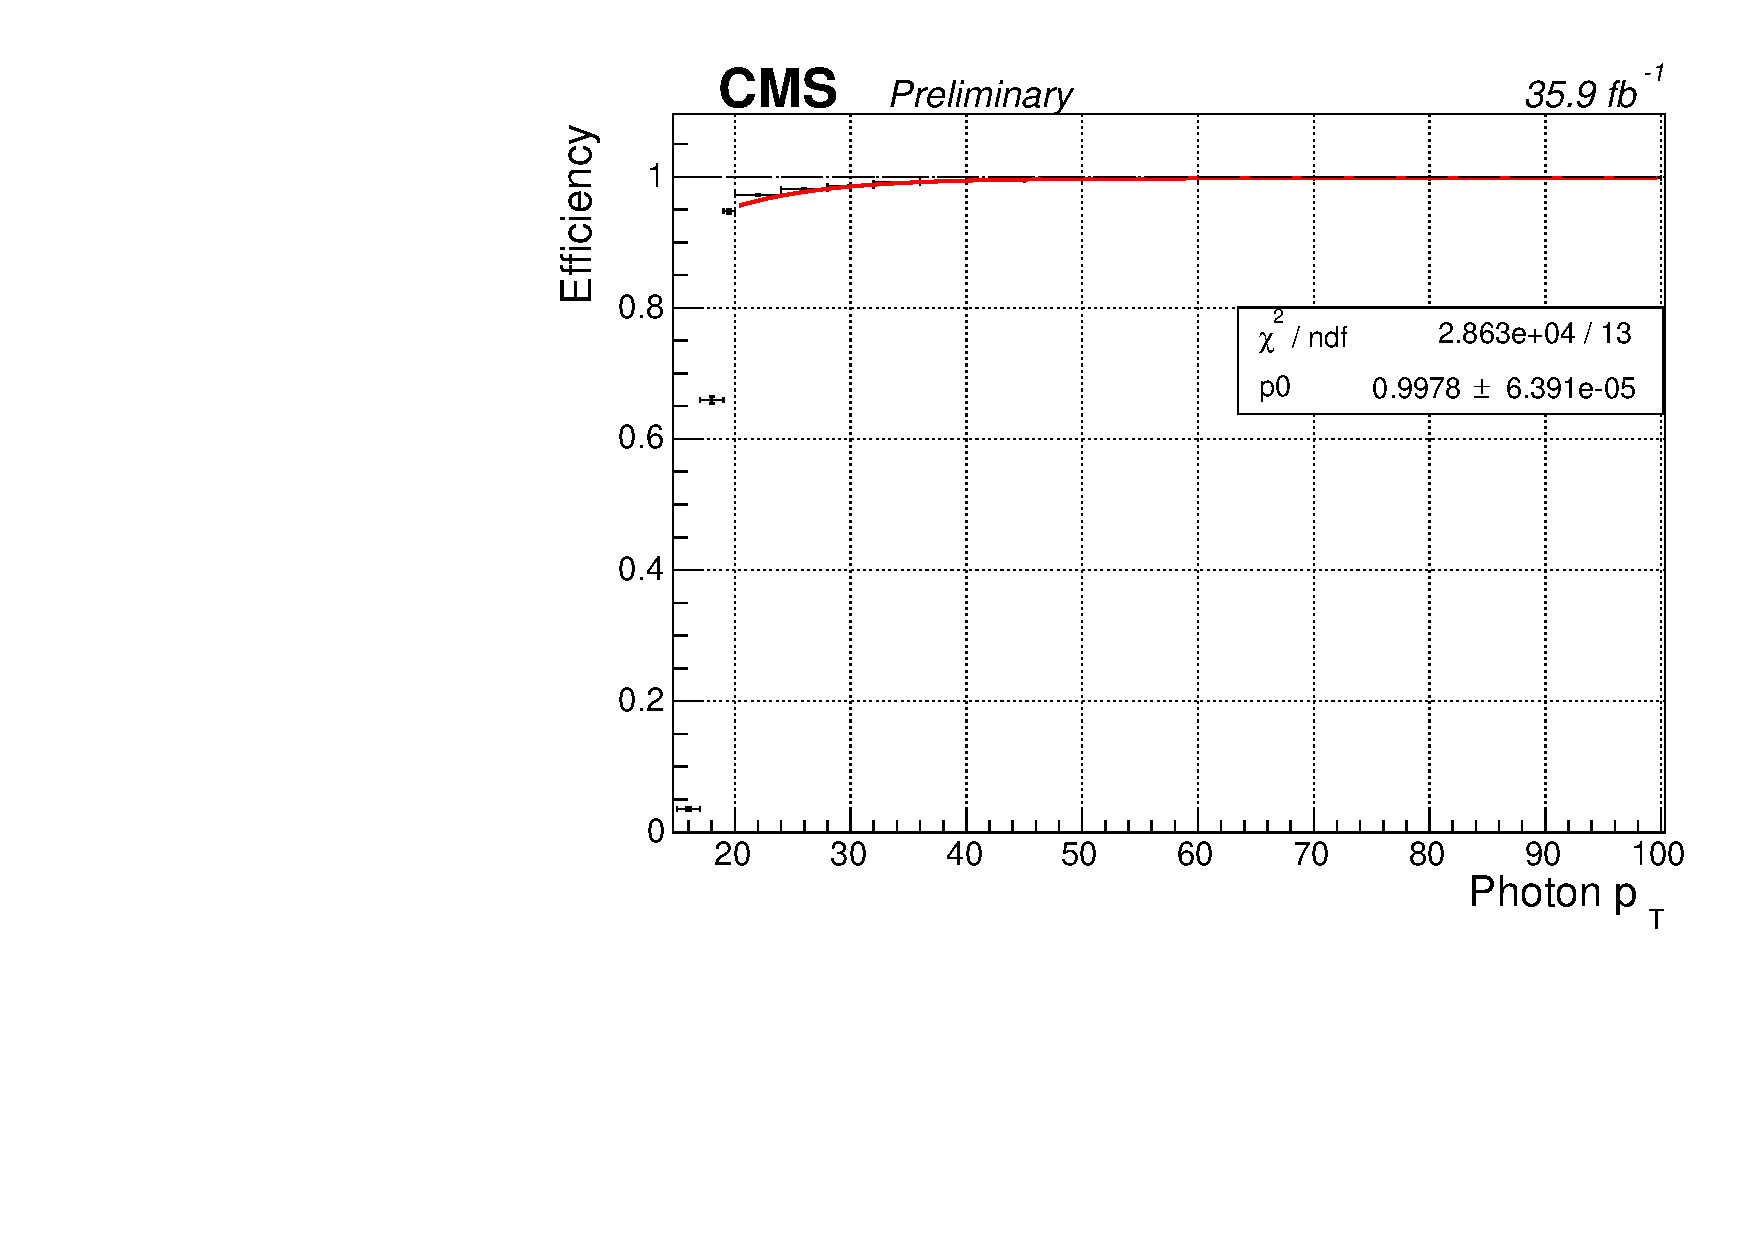
\includegraphics[width=0.9\textwidth]{Figures/Trigger/trailingEff.pdf}
\end{center}
\caption{Efficiency of the trailing leg of the primary analysis trigger with respect to photon \pT. 
For $\pT > 40$ GeV, the trigger is 99.8\% efficient.}
\label{fig:trailEff}
\end{figure*}

Finally, we calculated the efficiency of the trigger with respect to the diphoton invariant mass. For this calculation, we required two photons passing our analysis selection criteria, two photons satisfying the trailing leg of the trigger, and one photon passing the leading leg of the trigger. The efficiency was given by the number of diphoton events passing the full HLT path over the total number of diphoton events passing our requirements. The efficiency of the trigger as a function of invariant mass is shown in Figure~\ref{fig:InvMassEff}. For $m_{\gamma\gamma} > 100$ GeV, the trigger is 99.4\% efficient.

The efficiency of the trigger as a whole is the product of all three efficiencies. Two factors of the trailing leg efficiency are needed since both photons are required to pass that leg:
\begin{equation}
 \epsilon_{trig} = \epsilon_{lead} \times \epsilon_{trail}^2 \times \epsilon_{mass} = 97.2\%
\end{equation}

\begin{figure*}[h]
\begin{center}
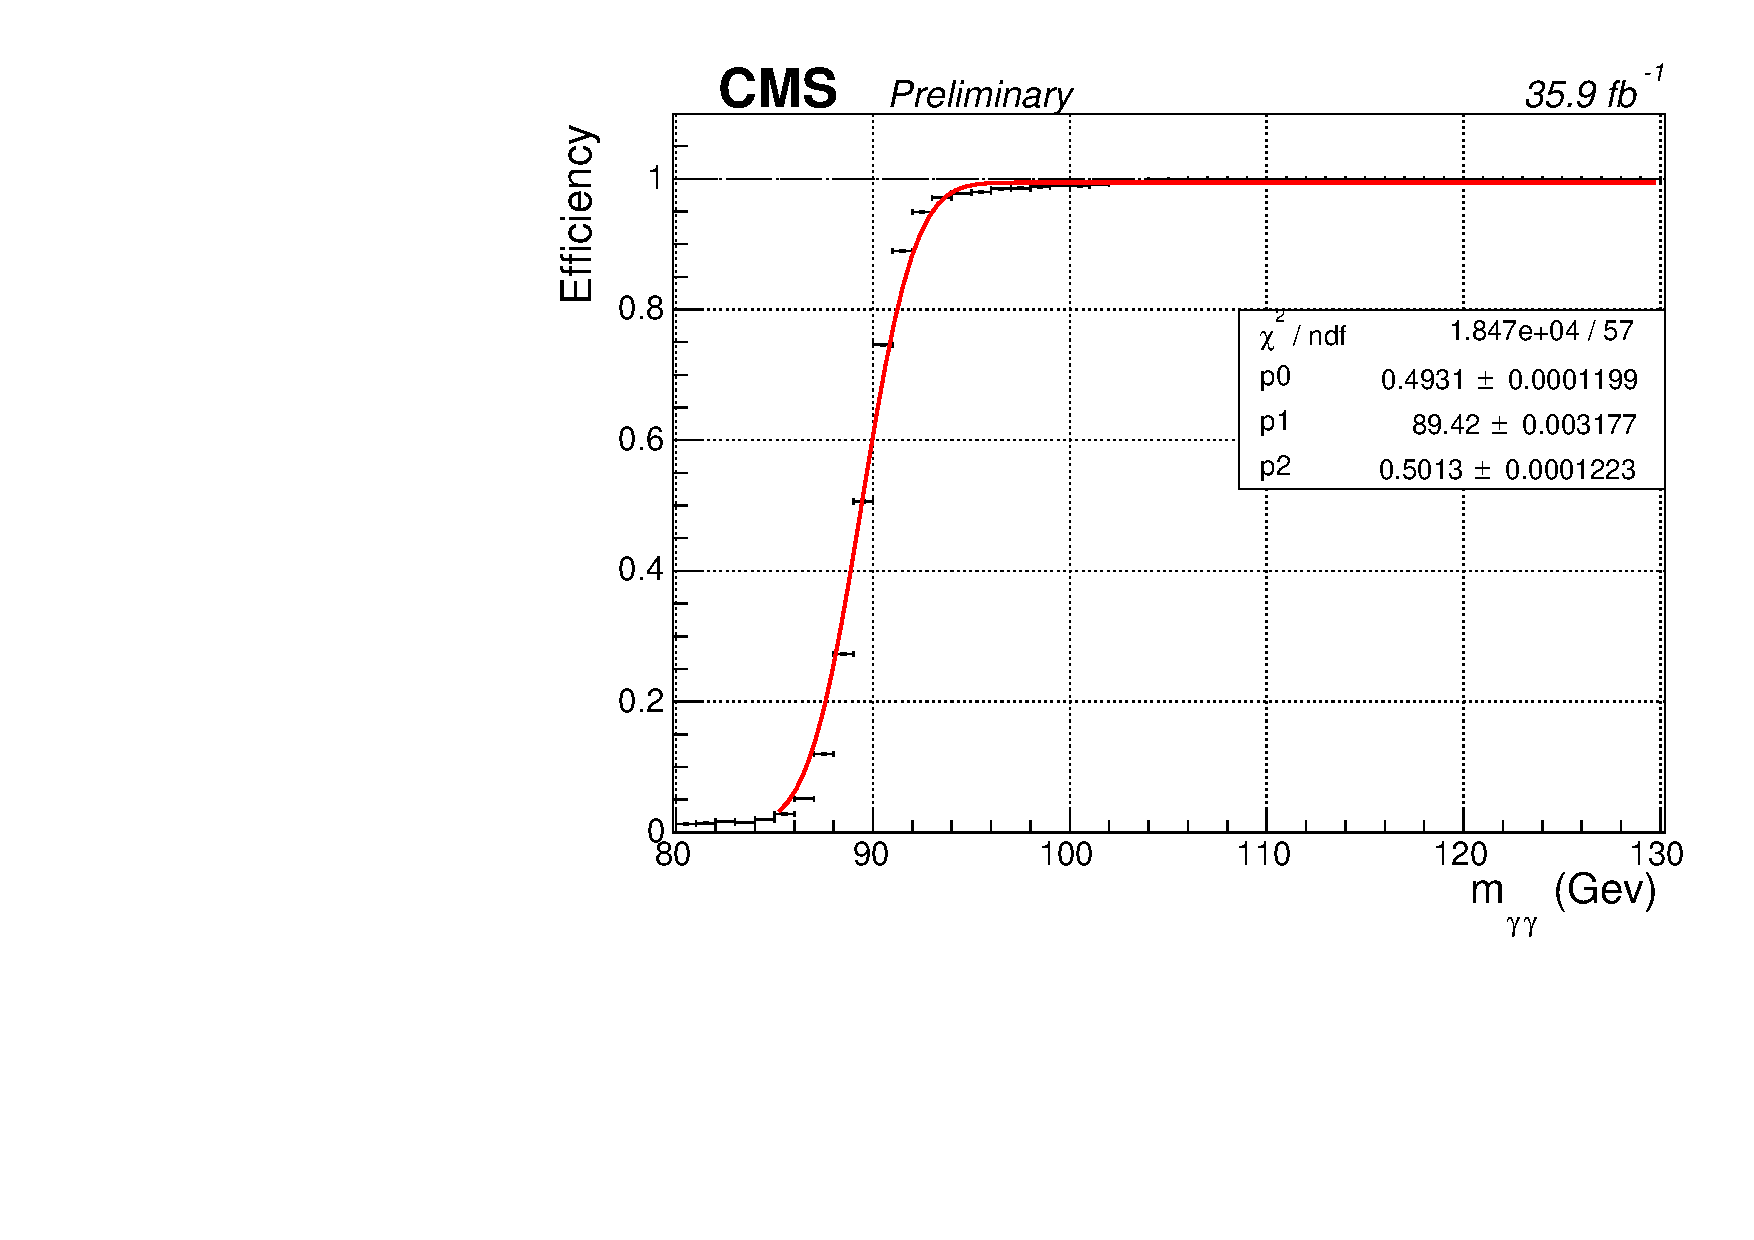
\includegraphics[width=0.9\textwidth]{Figures/Trigger/InvMassEff.pdf}
\end{center}
\caption{Efficiency of the primary analysis trigger with respect to the invariant mass of the diphoton system. 
For $m_{\gamma\gamma} > 100$ GeV, the trigger is 99.4\% efficient.}
\label{fig:InvMassEff}
\end{figure*}

\subsection{Efficiency of double electron trigger}
\label{sec:eeEff}
In the secondary trigger listed in Table~\ref{tab:triggers}, the pixel seed requirement is applied only to the trailing
leg of the trigger. This additional requirement results in a significantly lower overall efficiency for this leg. As shown in Figure~\ref{fig:controlTrailEff},
the trigger is only 90.4\% efficient for $\pT > 40$ GeV.
Since all other cuts are the same between the two triggers, however, the leading leg efficiency is the same as that shown in Figure~\ref{fig:leadEff}.
This results in an overall trigger efficiency of 79.8\% for the control trigger.

\begin{figure*}[h]
\begin{center}
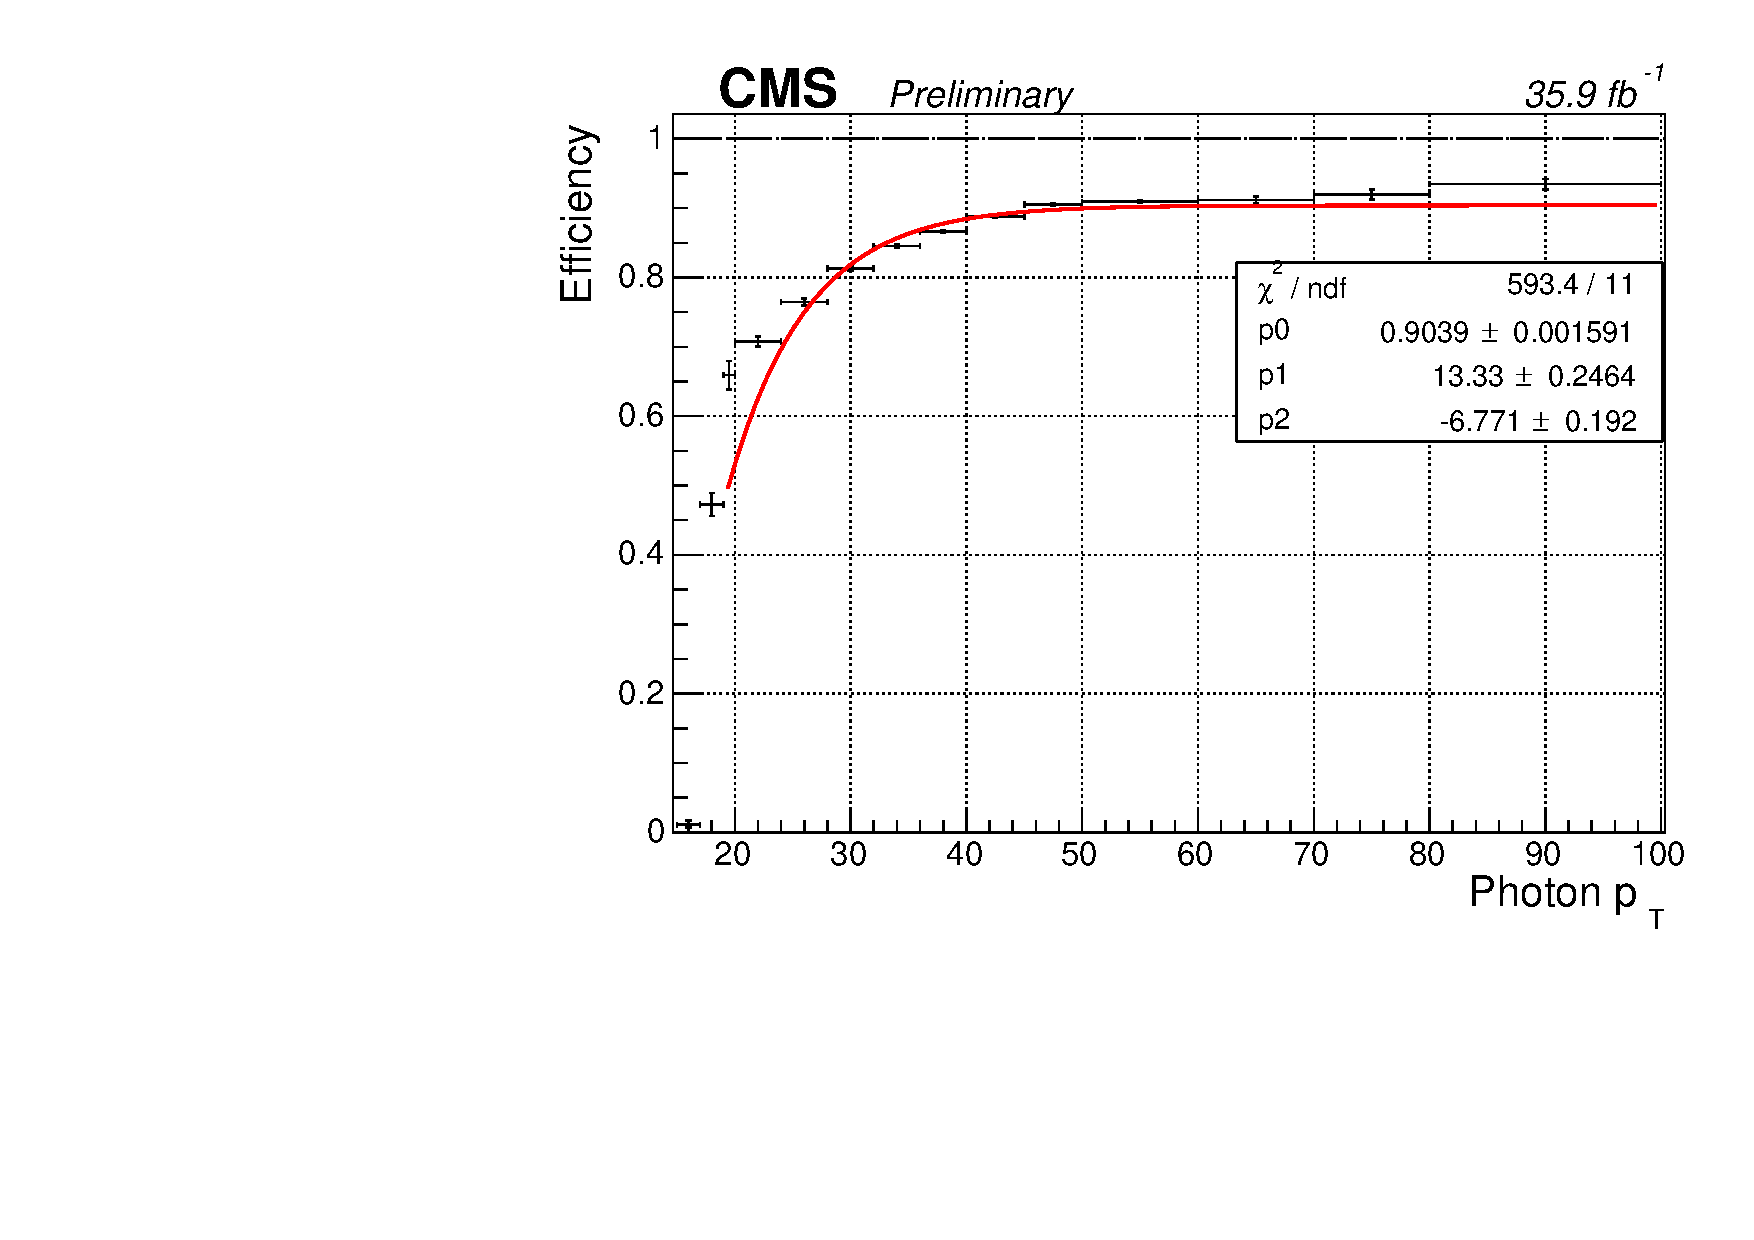
\includegraphics[width=0.9\textwidth]{Figures/Trigger/controlTrailingEff.pdf}
\end{center}
\caption{Efficiency of the trailing leg of the control trigger with respect to photon \pT. 
For $\pT > 40$ GeV, the trigger is 90.4\% efficient. The drop in efficiency with respect to the primary analysis 
trigger is caused by requiring both electromagnetic objects to be matched to a pixel seed.}
\label{fig:controlTrailEff}
\end{figure*}


  \chapter{DATA SETS AND SAMPLE DEFINITIONS}
\label{chap:EventSelect}

\section{Data samples}

As already mentioned, this analysis was performed using 35.9 \fbinv collected with the CMS detector in 2016. More specifically, the data sets listed in Table~\ref{tab:datasets} were used. These correspond to the reprocessing of the data that took place in February 2017 to include improved calibrations and performance corrections. The relevant ``golden JSON" file was used to specify which events passed all of the offline CMS data quality monitoring requirements: \\
Cert$\_$271036-284044$\_$13TeV$\_$23Sep2016ReReco$\_$Collisions16$\_$JSON.txt

\begin{table}[ht]
\caption{DATA SAMPLES}
\label{tab:datasets}
\begin{center}
\begin{tabular}{|>{\centering\arraybackslash}m{0.9\linewidth}|}
\hline
%\hline
%\textbf{Data sets} \\
\hline
/DoubleEG/Run2016B-03Feb2017$\_$ver2-v2/MINIAOD \\
/DoubleEG/Run2016C-03Feb2017-v1/MINIAOD \\
/DoubleEG/Run2016D-03Feb2017-v1/MINIAOD \\
/DoubleEG/Run2016E-03Feb2017-v1/MINIAOD \\
/DoubleEG/Run2016F-03Feb2017-v1/MINIAOD \\
/DoubleEG/Run2016G-03Feb2017-v1/MINIAOD \\
/DoubleEG/Run2016H-03Feb2017$\_$ver2-v1/MINIAOD \\
/DoubleEG/Run2016H-03Feb2017$\_$ver3-v1/MINIAOD \\      
\hline
\hline
\end{tabular}
 \justify{List of data samples used in this analysis.}
\end{center}
\end{table}

\section{MC samples}
\label{sec:MC}
Monte Carlo (MC) simulations are used for several purposes in this analysis. Simulations
of the signal processes are used to determine signal efficiencies, and
background process simulations are used for validation of the analysis performance
and to model the contribution from $Z\gamma\gamma\rightarrow\nu\nu\gamma\gamma$
events. 

There are three steps to create simulated events. The first step is the 
event generation, which simulates the primary scattering given an 
initial state ($p$-$p$ collisions in our case) and a list of final state particles.
To do so, a Monte Carlo (MC) method is utilized. The momentum phase-space
of the final particles is randomly sampled using a probability distribution
proportional to the differential cross section. For our analysis samples,
the \textsc{MadGraph}5~\cite{Alwall:2014hca} matrix-element generator was used.

The second step is to take the list of particles and corresponding 
momentum 4-vectors from the output of the event generator and 
perform parton showering. The partons are fragmented 
until the energy of each is below a set threshold. 
The new set of partons from the fragmentation 
are then hadronized. Additionally, the generation of initial state radiation
(ISR) occurs during this stage. 
We used the general-purpose event generator 
\PYTHIA8~\cite{Sjostrand:2007gs} for this step.

Finally, the last step is to simulate the detector response and to convert the list
of particles into detector observables. There are two approaches that were used
for the detector simulation: full simulation (FullSim) and fast simulation (FastSim). Both
rely on the \textsc{Geant}4 program.
In FullSim, the interactions are calculated from first principles using the full 
geometry of the detector modeled with as much detail as possible. In FastSim, 
the detector response is parameterized to avoid the time-consuming steps of FullSim. 
The modeling of the particle interactions 
with the tracker and calorimeters is replaced with libraries of particle showers~\cite{Abdullin:2011zz}.

The simulated tracker hits and calorimeter deposits are passed through the
full reconstruction algorithm that was previously described in
Chapter~\ref{sec:EventReconstruction} with one exception: in FastSim, the time-consuming track 
reconstruction uses the MC truth information rather than the simulated
detector hits. The final simulated output ends up in the same format as the output of the 
data reconstruction.

The full list of MC samples for this analysis is shown in Table~\ref{tab:MC}.
The background MC samples are generated with FullSim, and the signal samples 
are generated with FastSim. The signal simulation will be described in more detail in Section~\ref{sec:SimplifiedModels}. 

\begin{table}[ht]
\caption{MC SAMPLES FOR SIGNAL AND BACKGROUND}
\label{tab:MC}
\begin{center}
\begin{tabular}{|>{\centering\arraybackslash}m{0.9\linewidth}|}
\hline
\hline
\bf{SUSY Signal Samples}   \\         
\hline                                                                                         
\small{/SMS-T5Wg$\_$TuneCUETP8M1$\_$13TeV-madgraphMLM-pythia8/
          RunIISpring16MiniAODv2-PUSpring16Fast$\_$80X$\_$mcRun2$\_$
          asymptotic$\_$2016$\_$miniAODv2$\_$v0-v1/MINIAODSIM }\\
\hline
\small{/SMS-T5Wg$\_$mGo2150To2500$\_$TuneCUETP8M1$\_$13TeV-madgraphMLM-pythia8/
          RunIISpring16MiniAODv2-PUSpring16Fast$\_$80X$\_$mcRun2$\_$ 
          asymptotic$\_$2016$\_$miniAODv2$\_$v0-v1/MINIAODSIM }\\
\hline
\small{/SMS-T6Wg$\_$TuneCUETP8M1$\_$13TeV-madgraphMLM-pythia8/ 
 		     RunIISpring16MiniAODv2-PUSpring16Fast$\_$80X$\_$mcRun2$\_$ 
		     asymptotic$\_$2016$\_$miniAODv2$\_$v0-v1/MINIAODSIM }\\
\hline
\small{/SMS-T6Wg$\_$TuneCUETP8M1$\_$13TeV-madgraphMLM-pythia8/ 
          RunIISpring16MiniAODv2-PUSpring16Fast$\_$80X$\_$mcRun2$\_$ 
          asymptotic$\_$2016$\_$miniAODv2$\_$v0-v1/MINIAODSIM }\\
\hline                                               
\bf{Background MC Samples} \\ 
\hline                                                                                      
\small{/GJet$\_$Pt-40toInf$\_$DoubleEMEnriched$\_$MGG-80toInf$\_$TuneCUETP8M1$\_$13TeV$\_$Pythia8/ 
%\footnotesize{/GJet$\_$Pt-40toInf$\_$DoubleEMEnriched$\_$MGG-80toInf$\_$/
RunIISummer16MiniAODv2-PUMoriond17$\_$80X$\_$mcRun2$\_$ 
asymptotic$\_$2016$\_$TrancheIV$\_$v6-v1/MINIAODSIM} \\
\hline
\small{/ZGGToNuNuGG$\_$5f$\_$TuneCUETP8M1$\_$13TeV-amcatnlo-pythia8/
RunIISummer16MiniAODv2-PUMoriond17$\_$80X$\_$mcRun2$\_$
asymptotic$\_$2016$\_$TrancheIV$\_$v6-v1/MINIAODSIM }\\
\hline
\small{/DYJetsToLL$\_$M-50$\_$TuneCUETP8M1$\_$13TeV-madgraphMLM-pythia8/ 
RunIISpring16MiniAODv2-PUSpring16$\_$80X$\_$mcRun2$\_$
asymptotic$\_$2016$\_$miniAODv2$\_$v0$\_$ext1-v1/MINIAODSIM }\\                     
\hline
\hline
\end{tabular}
 \justify{List of MC samples used for signal and background studies.}
\end{center}
\end{table}

\section{Object definitions}
\label{sec:ObjSelect}

The MINIAOD data format of the data sets in Table~\ref{tab:datasets} includes lists of object candidates---photons, electrons, jets, etc.---from the reconstruction algorithms described in Chapter~\ref{sec:EventReconstruction}. Further refinements, however, are needed in the offline analysis to achieve the desired purities. For this analysis, the primary objects of interest are photons and electrons.

\subsection{Photon identification}
\label{sec:phoID}
Photons are required to satisfy \pT $> 40$ GeV in order to be in the region where the trigger is fully efficient. Due to the kinematics of the SUSY models under consideration, the majority of photons in SUSY events will be produced in the central region of the detector. For this reason, and to avoid the added complexity of the high-occupancy endcap, photons must be in the fiducial region of the ECAL barrel, $|\eta| < 1.4442$. 

We use the medium working point of the cut-based photon ID derived by the CMS $e/\gamma$ Physics Object Group (EGM POG). The medium working point was tuned to have an efficiency of 80\% and includes the following cuts:

\begin{itemize}
\item { H/E :} The ratio of the energy deposited in the HCAL tower directly behind the ECAL supercluster to the supercluster energy is required to be less than $0.0396$.
\item {$\sigma_{i{\eta}i{\eta}}$:} The log-fractional weighted width of the shower in i{$\eta$}-space is required to be less then $0.01022$.
\item {Particle Flow Charged Isolation :} The $\pT$ sum of all PF charged hadrons within a hollow cone of $0.02 < \Delta R < 0.3$ around the supercluster is required to be less than $0.441$~GeV.
\item {Particle Flow Neutral Isolation :} The $\pT$ sum of all neutral hadrons within a cone of $\Delta R <0.3$ around the supercluster
                                              is required to be less than $2.725 + (0.0148 \times \pT^{\gamma}) + (0.000017 \times (\pT^{\gamma})^2$).
\item {Particle Flow Photon Isolation :} The $\pT$ sum of all photons within a cone of $\Delta R < 0.3$,
                                             excluding a strip in $\eta$ of 0.015 around the supercluster, is required to be less than $2.5718 + (0.0047 \times \pT^{\gamma})$.
\end{itemize}

All of the isolation values are corrected to remove pileup contributions as described in Section~\ref{sec:pileup}. The corrected value of isolation $I_{\mathrm{corr.}}$ is given by 
\begin{equation}
I_{\mathrm{corr.}} = I_{\mathrm{uncorr.}} - \rho A_{\mathrm{eff}}
\end{equation}
The values of the effective area for each isolation correction are listed in Table~\ref{tab:EA}.

\begin{table}[ht]
    \caption{EFFECTIVE AREAS FOR ISOLATION CORRECTIONS}
    \centering
    \begin{tabular}{ | c | c | c | c |}
        \hline
        	\hline
        \textbf{$|\eta|$ Range} & \textbf{Photon Iso} & \textbf{Neutral Hadron Iso} & \textbf{Charged Hadron Iso} \\ [0.5ex]
        \hline
        	$|\eta| < 1.0 $                 & 0.120   &  0.0597 & 0.0360\\
	$ 1.0 < |\eta| < 1.479 $   & 0.1107 & 0.0807 & 0.0377 \\
		 \hline
           \hline
    \end{tabular}
    \label{tab:EA}
    \justify{Effective areas used in the definition of photon, charged hadron, and neutral hadron isolation values. }
\end{table}
In addition to the medium ID criteria, photons must satisfy $R_9 > 0.5$. This is imposed to ensure that photons pass the trigger (which includes an $R_9$ requirement) with a high efficiency. Finally, to distinguish photon candidates from electrons, photons are required to pass a pixel seed veto (PSV). That is, photons must not be matched to a pixel seed, defined as at least two hits in the pixel detectors consistent with a charged particle trajectory which would arrive at the ECAL.

\subsection{Electron identification}
\label{sec:eleID}
As already mentioned, electrons---particularly electrons from $Z\rightarrow ee$ decays---are a useful proxy for photons because of the similar response in the ECAL. We define an electron as a candidate object satisfying all of the requirements of Section~\ref{sec:phoID} but failing the PSV. Using the same ID requirements for electrons and photons enables us to define control regions with electrons without introducing any biases between the control region and the candidate diphoton sample we are trying to model. By reversing the pixel seed veto, we make the electron and photon selections orthogonal and avoid double-counting objects. The requirements for photons and electrons are listed in detail in Table~\ref{tab:ID}. 

\subsection{Fake identification}
\label{sec:fakeID}
In addition to photons and electrons, a third, orthogonal category referred to as ``fake" photons is defined. 
Fakes are primarily electromagnetically-rich jets that have been misidentified as photons. As will be described in Chapter~\ref{chap:DataAnalysis},
the predicted QCD background is derived using a double fake control sample.

Table~\ref{tab:fakeID} lists the ID criteria for fakes.
The fake definition is taken from a photon ID sideband. Fakes are required to
% must pass all of the photon identification criteria described in Section~\ref{sec:phoID}, except they
fail either the \sigmaietaieta or the charged hadron isolation requirement of the photon ID. 
This ensures that the photon and fake selection criteria are orthogonal. Upper bounds
(0.015 and 25 for \sigmaietaieta and charged hadron isolation, respectively)
are placed on the values of both variables to ensure that the fake definition does not differ too much 
from the nominal photon definition. 

In addition, fakes must satisfy $0.5 < R_9 < 0.9$. Using the more inclusive cut $R_9 > 0.5$
resulted in significant contamination from SUSY events in the double fake control sample. To
counteract the effect this cut has on the already-limited fake statistics, the
neutral hadron isolation and photon isolation cuts are loosened significantly.

\begin{table}[ht]
    \caption{PHOTON AND ELECTRON ID CRITERIA}
    \centering
    \begin{tabular}{ |>{\centering\arraybackslash}m{0.25\linewidth}| >{\centering\arraybackslash}m{0.25\linewidth} >{\centering\arraybackslash}m{0.25\linewidth} |}
        \hline
        	\hline
        \textbf{ID Requirement} & \textbf{Photons} & \textbf{Electrons} \\ [0.5ex]
        \hline
        	Pixel seed veto    & \multicolumn{1}{c|}{Applied} & \multicolumn{1}{c|}{Reversed} \\
	\hline
	\sigmaietaieta   & \multicolumn{2}{c|}{$ < 0.01022 $} \\
	Charged hadron iso. & \multicolumn{2}{c|}{$ < 0.441$} \\
	\hline
	Photon iso. & \multicolumn{2}{c|}{$ < 2.571 +0.0047~\pt$} \\
	Neutral hadron iso.   &  \multicolumn{2}{c|}{$ < 2.2725 + 0.0148~\pt+0.000017~\pt^2$} \\
        $R_9$                      & \multicolumn{2}{c|}{$ > 0.5$} \\
        H/E                     & \multicolumn{2}{c|}{$ < 0.0396$} \\
           \hline
           \hline
    \end{tabular}
    \label{tab:ID}
    \justify{Photon and electron identification criteria used to define the signal and control samples for this analysis. 
    The definitions of each of the variables can be found in 
    Section~\ref{sec:phoID}.}
\end{table}


\begin{table}[ht]
    \caption{FAKE ID CRITERIA}
    \centering
    \begin{tabular}{ |>{\centering\arraybackslash}m{0.25\linewidth}| >{\centering\arraybackslash}m{0.5\linewidth} |}
        \hline
        	\hline
        \textbf{ID Requirement} & \textbf{Fakes} \\ [0.5ex]
        \hline
        	Pixel seed veto    & Applied\\
	\hline
	\sigmaietaieta   & $0.01022 < \sigmaietaieta < 0.015 $\\
	Charged hadron iso. & $ 0.441 <$ Iso $< 25$\\
	\hline
	Photon iso. &$ < 15 +0.0047~\pt$\\
	Neutral hadron iso. & $< 15 + 0.0148~\pt+0.000017~\pt^2$\\
        $R_9$    & $0.5 < R_9 < 0.9$ \\
        H/E      & $ < 0.0396$\\
           \hline
           \hline
    \end{tabular}
    \label{tab:fakeID}
    \justify{Identification criteria for ``fakes." Fakes come from a photon ID sideband and are primarily
    jets that have been misidentified as photons. The definitions of each of the variables can be found in 
    Section~\ref{sec:phoID}.}
\end{table}

\subsection{Object cleaning}
\label{sec:ObjCleaning}

In order to avoid double counting particles, a set of object cleaning rules are applied. 
First, because muons are reconstructed with a higher purity than any other particle, 
any electromagnetic object (photon, electron, or fake) that is within \dR~$< 0.3$ of a muon candidate is removed.
Second, any photon that overlaps within \dR~$< 0.3$ of an electron is removed. Finally, if a fake overlaps with an electron or 
photon candidate within \dR~$< 0.4$, the fake candidate is removed. The larger \dR~separation for fakes is due to the fact
that fakes are primarily jets and jets are reconstructed using the \antikt algorithm with a distance
parameter of 0.4, as described in Section~\ref{sec:Jet}.  

\subsection{Lepton veto}
\label{sec:lepVeto}

In addition to the cuts described above, any event that contains additional muons or electrons is vetoed. 
No additional leptons are present in the SUSY signals of interest, so applying a lepton veto will not hurt our signal sensitivity.
More importantly, by vetoing on the presence of additional leptons, our analysis becomes orthogonal to other CMS searches for
gauge-mediated supersymmetry breaking with photons in the final state. 
%As described in Section~XX, this is particularly important for the combination paper.

\section{Signal region and control samples}
\label{sec:samples}
After the individual objects are defined and identified, each event is sorted into one of four exclusive categories based on the electromagnetic objects with the highest \pT in the event. Events with two photons comprise the signal diphoton sample, referred to as the $\gamma\gamma$ sample. Events with two electrons, one electron and one photon, or two fakes are categorized as $ee$, $e\gamma$, or $ff$ events, respectively. In each case, the two electromagnetic objects are required to be separated by \dR~$ > 0.6$. 

The  $\gamma\gamma$, $ff$, and $e\gamma$ samples are required to pass the primary trigger described in Section~\ref{sec:analysisTrig}. 
In order to ensure that the events pass the trigger with a high efficiency, the invariant mass of the two electromagnetic objects is required to be greater than 105 GeV. 
The $ee$ sample, on the other hand, is collected using the control trigger listed in Table~\ref{tab:triggers} and is required to satisfy $75 < m_{ee} < 105$ GeV. Chapter~\ref{chap:DataAnalysis} will explain in detail how each of these samples is used in this analysis.

%%%%%%%%%%%%%%%%%%%%%%%%%%%%%%%%%%%%%%%
%%%%%%%%%%%%%%%%%%%%%%%%%%%%%%%%%%%%%%%
%%%%%%%%%%%%%%%%%%%%%%%%%%%%%%%%%%%%%%%

\section{Photon ID scale factor}
\label{sec:phoSF}
The efficiency of the photon ID is measured via the tag-and-probe method in $Z \rightarrow ee$ events~\cite{phoPerf8TeV}. 
The procedure is similar to the one described in Chapter~\ref{chap:Trigger} for calculating the trigger efficiency.
A sample of $Z \rightarrow ee$ events is collected using a single electron trigger. One electron is used as the tag, and 
one electron is used as the probe. The efficiency is given by the number of probes that pass the photon ID over the 
total number of tag and probe pairs. This value is computed in both data and simulation,
and the ratio of the two efficiencies is referred to as the scale factor. 

For this analysis, the official
scale factors calculated by the EGM POG for Moriond 2017 were used.
The scale factors from the EGM POG are calculated in bins of photon \pt and
$\eta$. These are shown in Figure~\ref{fig:SF} along with the
associated uncertainties~\cite{SF_twiki}.

\begin{figure*}[htbp]
    \centering
    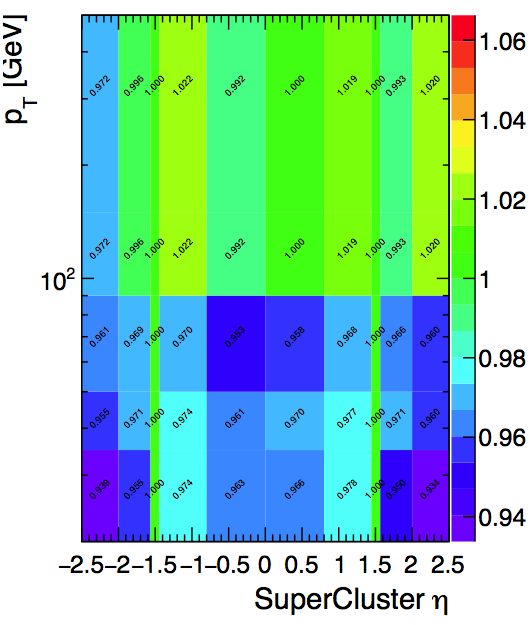
\includegraphics[width=0.49\textwidth]{Figures/EventSelect/scalefactors.png}
    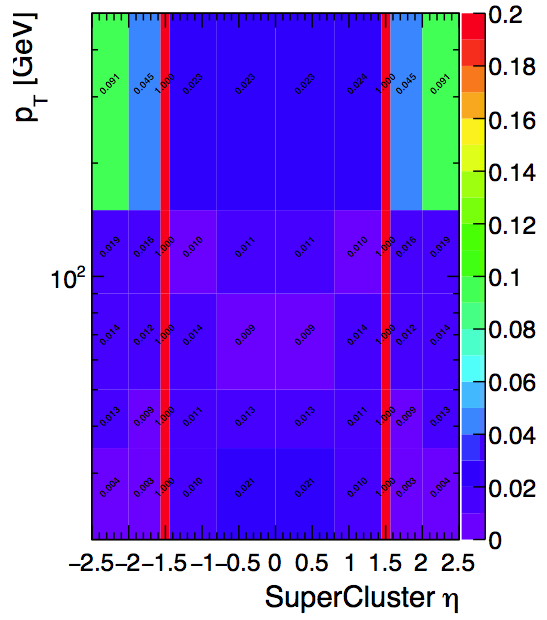
\includegraphics[width=0.49\textwidth]{Figures/EventSelect/sf_errors.png}
    \caption[Calculated scale factors and uncertainties 
      in bins of photon \pt and $\eta$.]
    {Calculated scale factors (left) and uncertainties (right)
      in bins of photon \pt and $\eta$.}
    \label{fig:SF}
\end{figure*}

Rather than using the full map of scale factors shown in Figure~\ref{fig:SF},
we compute a weighted average over all photons passing our selection criteria
in each SUSY signal mass point.
The average scale factors and uncertainties are shown in Figure~\ref{fig:SFmap}.

\begin{figure*}[htbp]
    \centering
    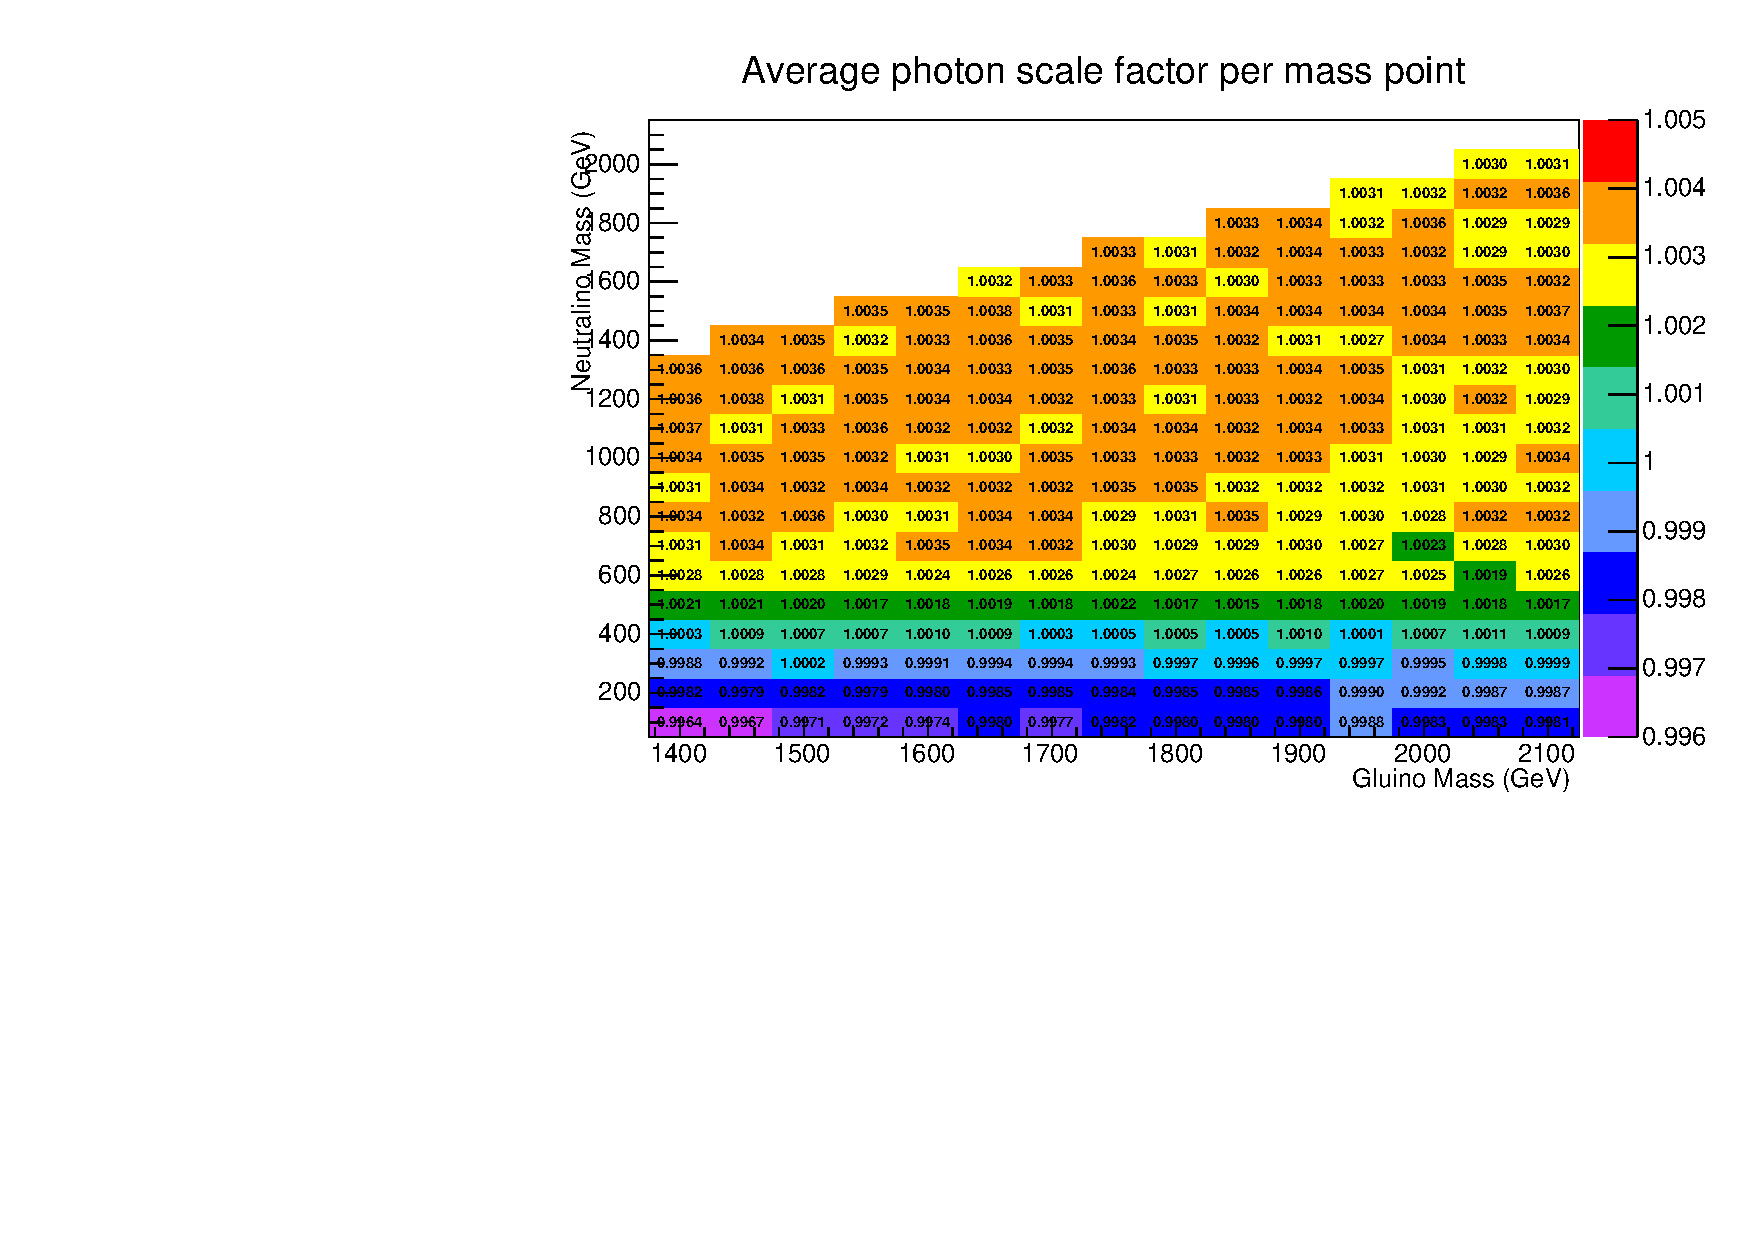
\includegraphics[width=0.8\textwidth]{Figures/EventSelect/sfmap.pdf}
    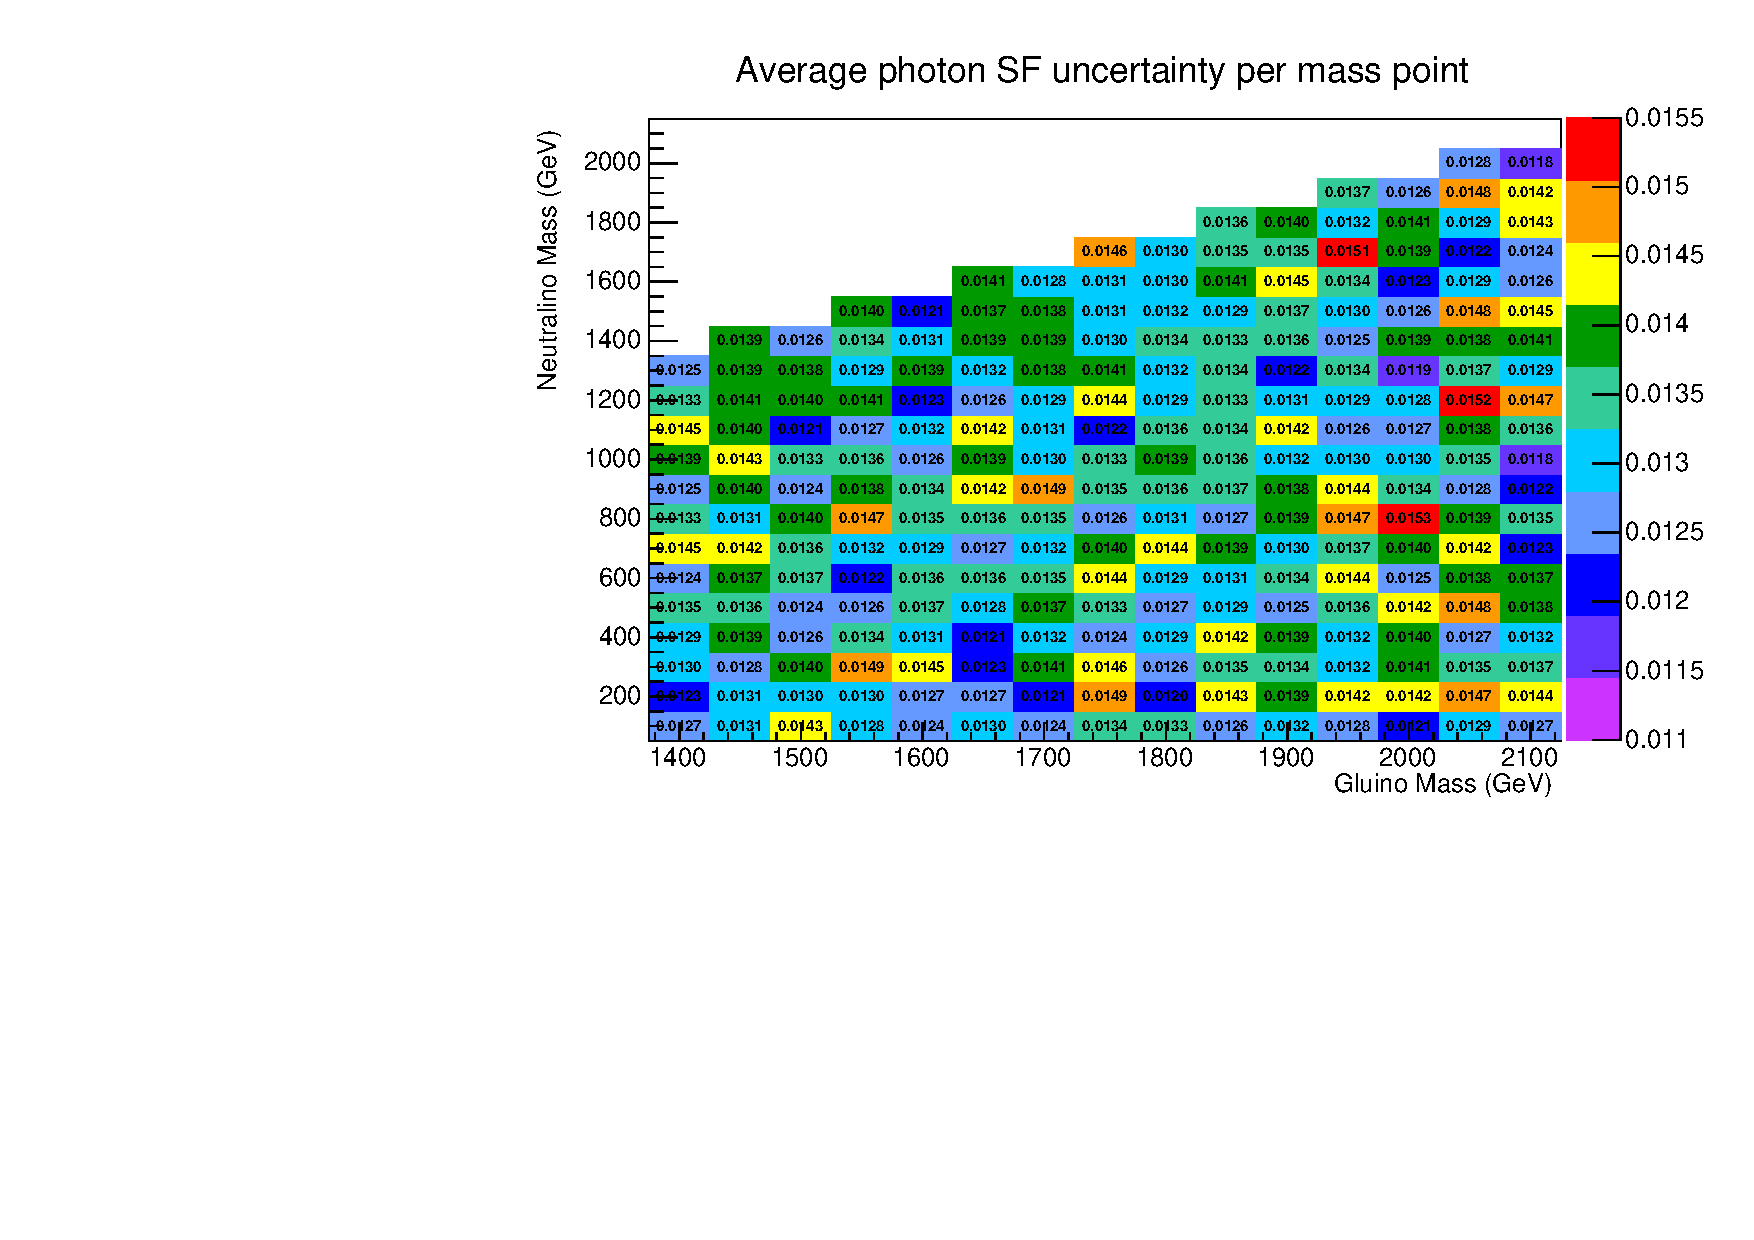
\includegraphics[width=0.8\textwidth]{Figures/EventSelect/sfmap_errors.pdf}
    \caption[Scale factors and uncertainties 
      averaged over all photons in each bin in the neutralino
      versus gluino mass plane.]
      {Scale factors (top) and uncertainties (bottom)
      averaged over all photons in each bin in the neutralino
      versus gluino mass plane.}
    \label{fig:SFmap}
\end{figure*}

The final value used in the analysis was an average over the mass
points shown in Figure~\ref{fig:SFmap}:
\begin{equation}
  \textrm{Photon Scale Factor} = 1.002\pm0.013
\end{equation}

\subsection{Scale factor for pixel seed veto}
\label{sec:PSV_SF}
Our prescription for photon identification is nearly identical to that for
electron identification, differing only by the presence or absence of a seed
track in the pixel detector. The efficiency of the pixel seed veto
for photons cannot be determined from the tag-and-probe method described above
and must be obtained from photons in $Z\rightarrow \mu\mu\gamma$
events. Again we use the official scale factor calculated by the
EGM POG:
\begin{equation}
  \textrm{Pixel Seed Veto Scale Factor} = 0.998\pm0.013
\end{equation}
Since our candidate sample requires two photons in the final state,
two factors of both values are used.


\subsection{Scale factor for $R_9$ requirement}
\label{sec:R9SF}
The photon ID used in this analysis differs from the official POG recipe in one aspect: we apply an $R_9 > 0.5$ requirement on top of the medium ID due to the presence of an $R_9$ cut in our analysis trigger. A check was performed to make sure that the $R_9$ requirement does not change the photon scale factors. The results of this study are shown in Figure~\ref{fig:R9SF}. The data/MC scale factors are all consistent with unity. We therefore choose to simply use the official scale factors described above, rather than applying any additional corrections.

\begin{figure*}[htbp]
    \centering
    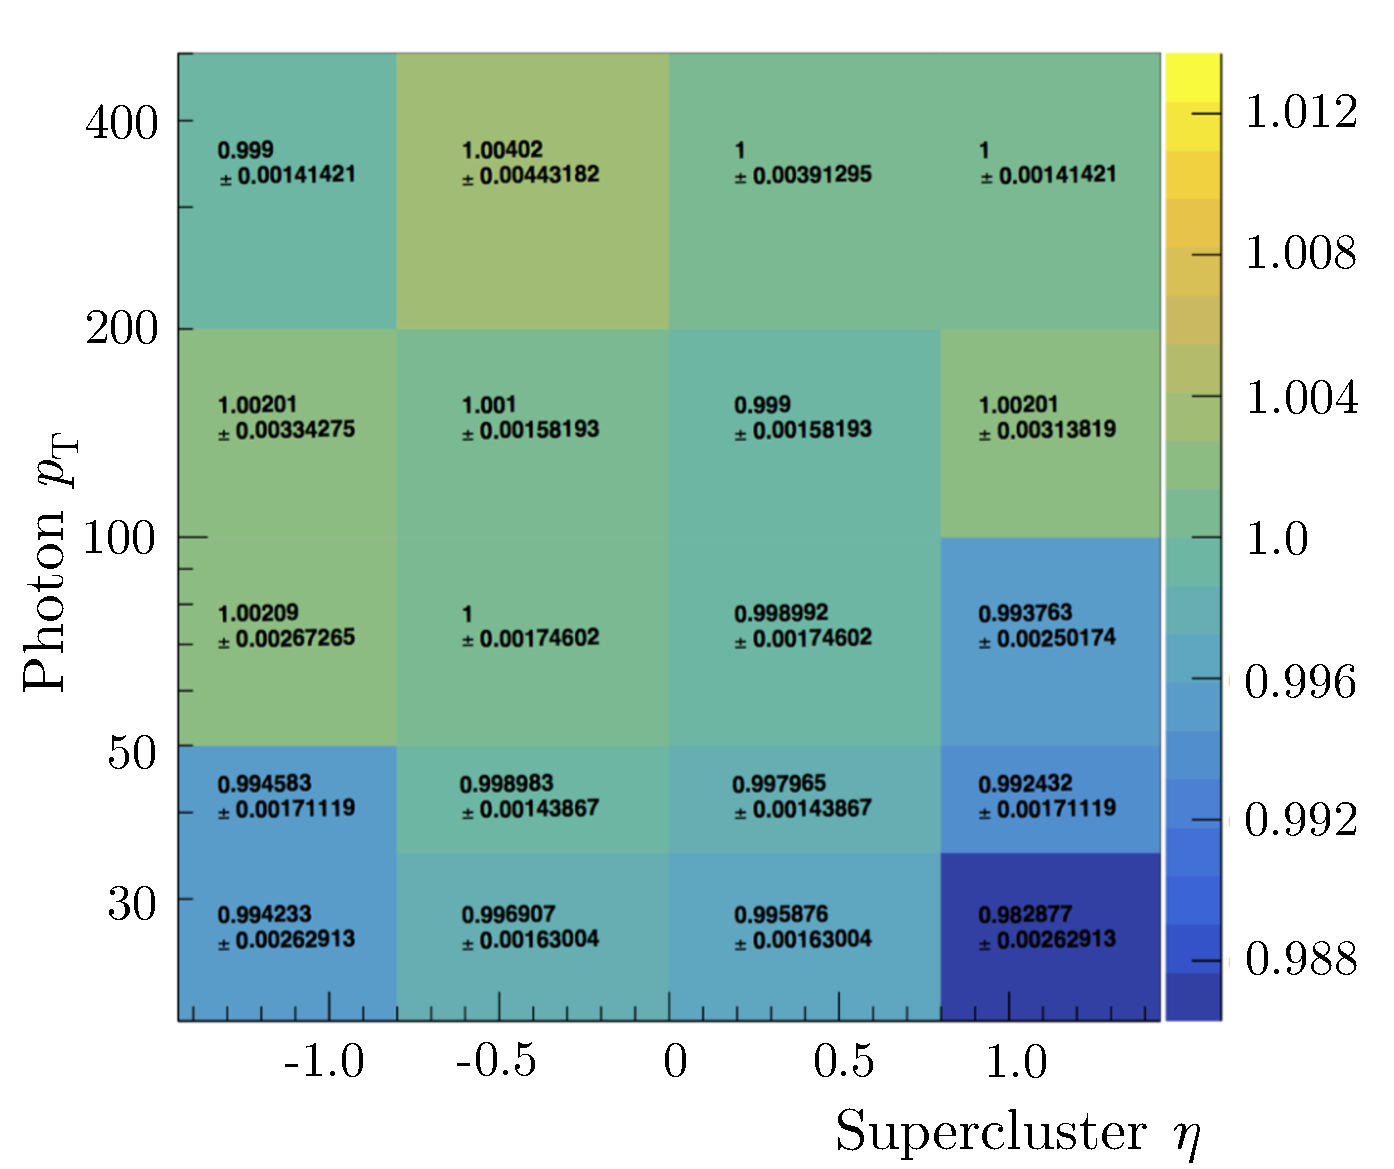
\includegraphics[width=0.9\textwidth]{Figures/EventSelect/R9SF.pdf}
    \caption[Scale factor for applying $R_9 > 0.5$ on top of the cut-based medium photon ID.]
    {Scale factor for applying $R_9 > 0.5$ on top of the cut-based medium photon ID.
    The scale factors are consistent with unity in all bins. Therefore, no additional corrections are applied to
    the scale factors described in Section~\ref{sec:phoSF}.}
    \label{fig:R9SF}
\end{figure*}



  \chapter{DATA ANALYSIS AND BACKGROUND ESTIMATION METHODS}
\label{chap:DataAnalysis}

\section{Overview}

There are several standard model processes that can mimic our signal events. The largest background contribution comes from quantum chromodynamics (QCD) processes. These are primarily multi-jet events, where electromagnetically-rich jets are misidentified as photons, but can also include processes with true photons either from associated photon production or initial-state radiation. In both cases, there is no inherent \ETmiss in the event. Instead, the measured \ETmiss is actually the result of mismeasured hadronic activity. As described in Section~\ref{sec:QCD}, this background is estimated in an entirely data-driven way using a control region derived from a sideband of our photon ID. 

The second-largest background is the electroweak (EWK) background. This background is comprised of $W\gamma$ or $W$+jet events where $W\rightarrow e \nu$. In this case, there is inherent \ETmiss from the neutrino, and these events can mimic our signal topography if the electron is misidentified as a photon. By measuring the misidentification rate in data, we can use an $e\gamma$ control sample to estimate the contribution from the EWK background. The EWK background estimation method is described in detail in Section~\ref{sec:EWK}. 

Finally, there is an irreducible background from $Z\gamma\gamma\rightarrow\nu\nu\gamma\gamma$ events. This background is modeled via simulation and is described in Section~\ref{sec:Zgg}.

%%%%%%%%%%QCD Methodology %%%%%%%%%%%%%%%%%%

\section{QCD background}
\label{sec:QCD}

Due to the large QCD cross section, the most significant background for this analysis comes from QCD events without true \ETmiss and without two real photons. 
The observed \ETmiss is the result of mismeasured hadronic activity, and in most cases the ``photons" are misidentified jets with a large electromagnetic component.

To estimate the contribution from the QCD background in our signal region, we use the ``fake" object selection that was described in Section~\ref{sec:ObjSelect}. The fake identification criteria is orthogonal to the nominal photon identification, and therefore provides a sideband that can be used as a control region. The \ETmiss tail of the QCD background is modeled using a ``fake-fake" (``$ff$") control sample made up of events with two fakes that pass the additional criteria outlined in Section~\ref{sec:samples}.

\subsection{Di-EM \pT reweighting}
\label{sec:diempt}

Because the \ETmiss in the QCD background and the $ff$ control sample arises from poorly measured hadronic activity, it is important that the amount of hadronic activity in the control sample matches that of the $\gamma\gamma$ events we are trying to model.

To account for potential differences between the samples, we define a variable referred to as the ``\diempt" of an event. Di-EM \pT is defined as the magnitude of
the vector sum of the transverse momentum of the two electromagnetic objects (photons, electrons or fakes):
\begin{equation}
 \vec{p}_\mathrm{T}^{\, \,\mathrm{di\mbox{-}EM}}=\vec{p}_{\mathrm{T}1}+\vec{p}_{\mathrm{T}2}
 \label{equ:diempt}
\end{equation}

As illustrated in Figure~\ref{fig:diempt}, the \diempt variable is used as a measure of the total hadronic recoil. Because CMS measures the energies of electromagnetic objects with greater precision than the energy of jets, this variable is a more accurate representation of the hadronic recoil than simply adding up the transverse momentum of the jets themselves. 

\begin{figure*}[h]
\begin{center}
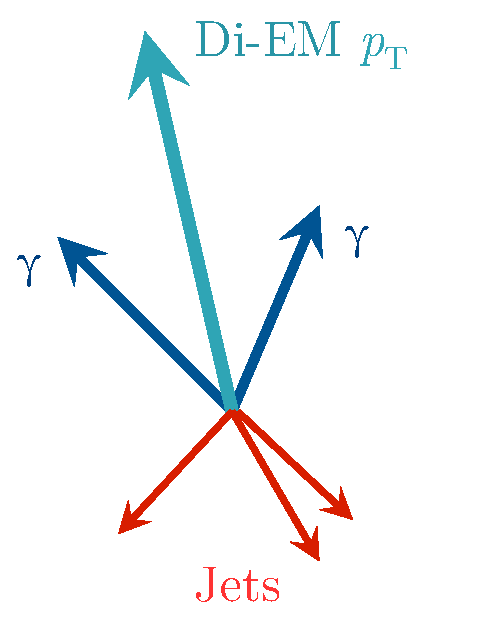
\includegraphics[width=0.3\textwidth]{Figures/DataAnalysis/Diempt.pdf}
\end{center}
\caption{The \diempt vector, shown in light blue, is the vector sum of the \pT of the two photons in the event, shown in blue. The magnitude of the \diempt vector is used to model the hadronic recoil, shown in red. }
\label{fig:diempt}
\end{figure*}

The \diempt distributions for the $\gamma\gamma$ candidate sample and the $ff$ control sample are shown in Figure~\ref{fig:ggffDiempt}. The $ff$ events are reweighted using the $\gamma\gamma$/$ff$ ratios displayed in the ratio plot of Figure~\ref{fig:ggffDiempt}. The $ff$ \ETmiss distribution is normalized to the \ETmiss $<~50$ GeV region of the $\gamma\gamma$ sample, where signal contamination is minimal. 

\begin{figure*}[h]
\begin{center}
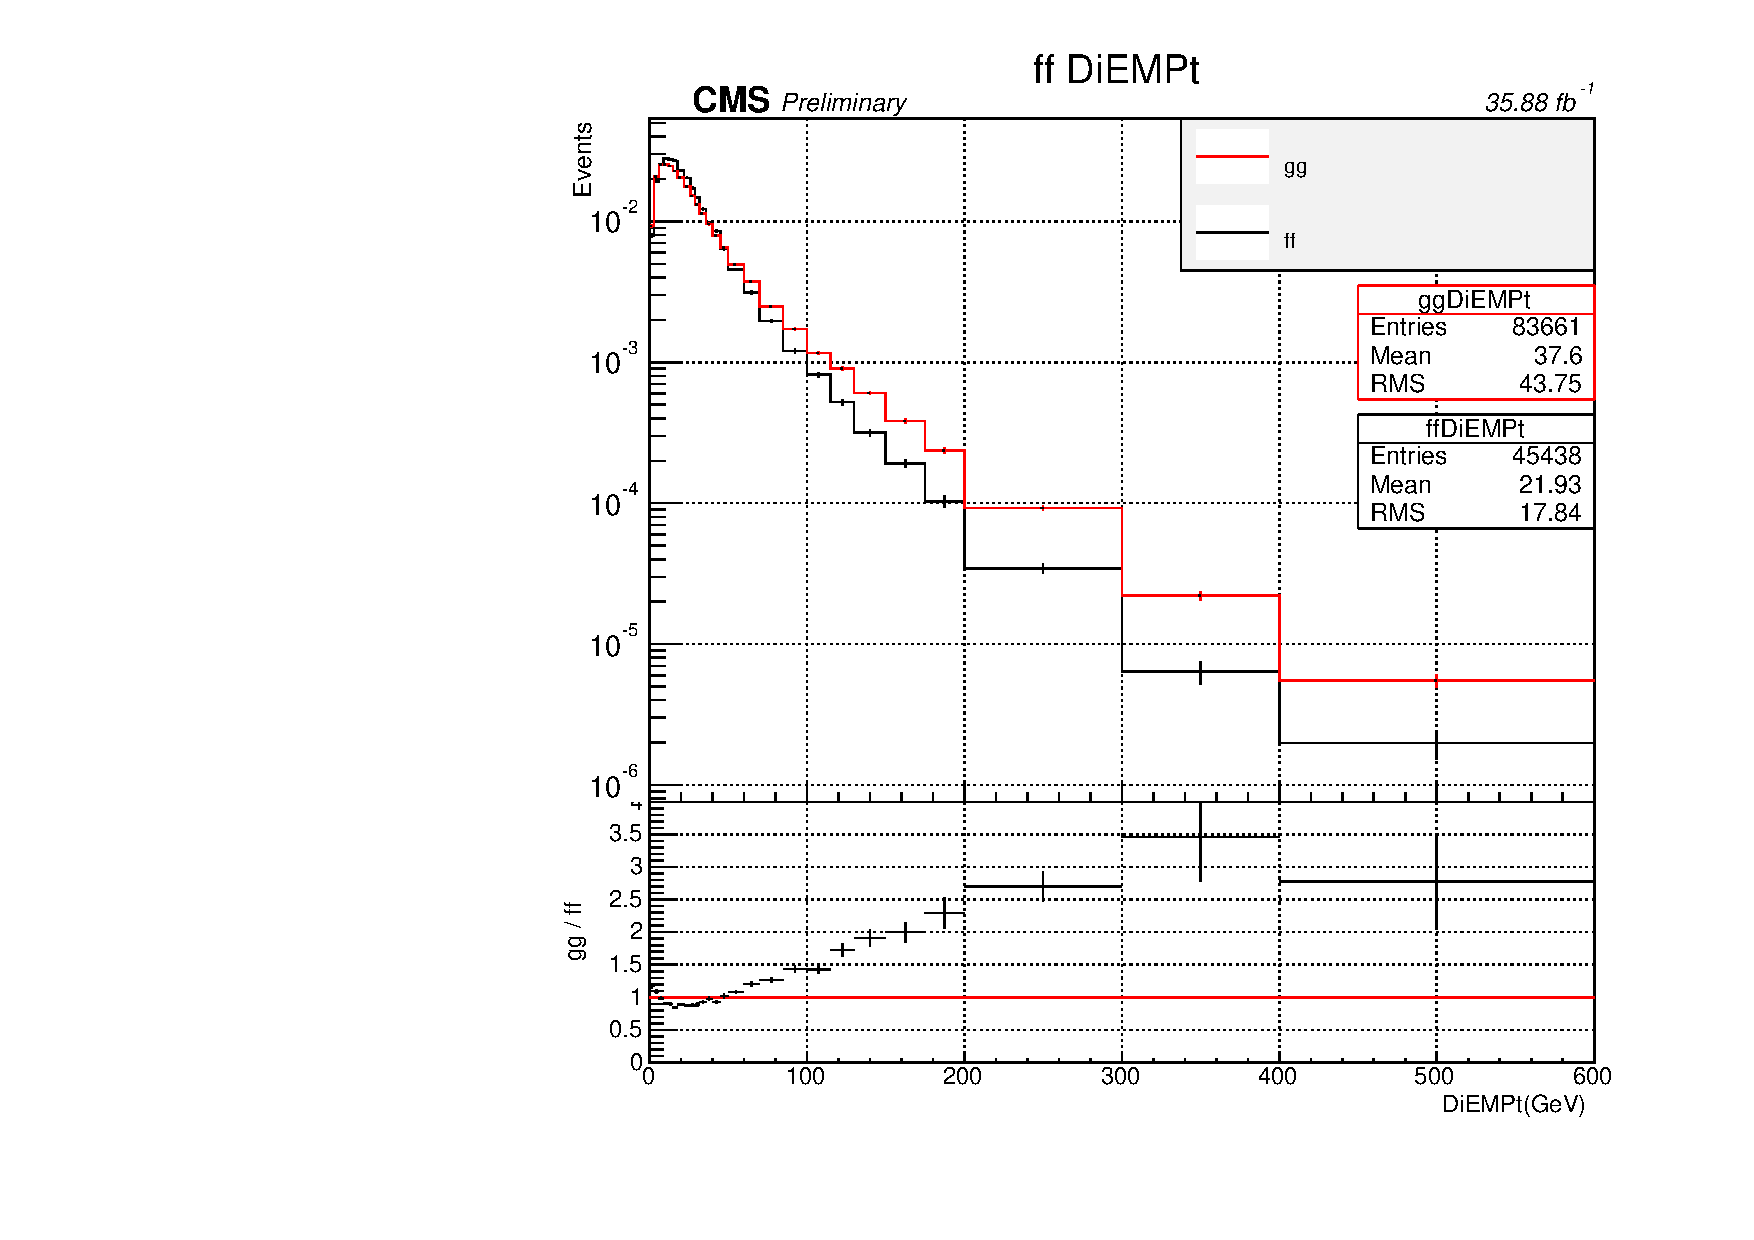
\includegraphics[width=0.9\textwidth]{Figures/DataAnalysis/ggffDiempt.pdf}
\end{center}
\caption{\Diempt distributions of the $ff$ control sample (black) and the $\gamma\gamma$ candidate sample (red). The ratio plot on the bottom shows the $\gamma\gamma$/$ff$ ratios that are used to reweight the $ff$ \ETmiss distribution. }
\label{fig:ggffDiempt}
\end{figure*}

The unweighted $ff$ and $\gamma\gamma$ \ETmiss distributions are shown in Figure~\ref{fig:ggffUnweighted}. A comparison between the unweighted and \diempt reweighted $ff$ \ETmiss distributions is shown in Figure~\ref{fig:compareUnweighted}. Finally, Figure~\ref{fig:ggffReweighted} compares the reweighted $ff$ \ETmiss distribution to the candidate $\gamma\gamma$ \ETmiss distribution.

\begin{figure*}[h]
\begin{center}
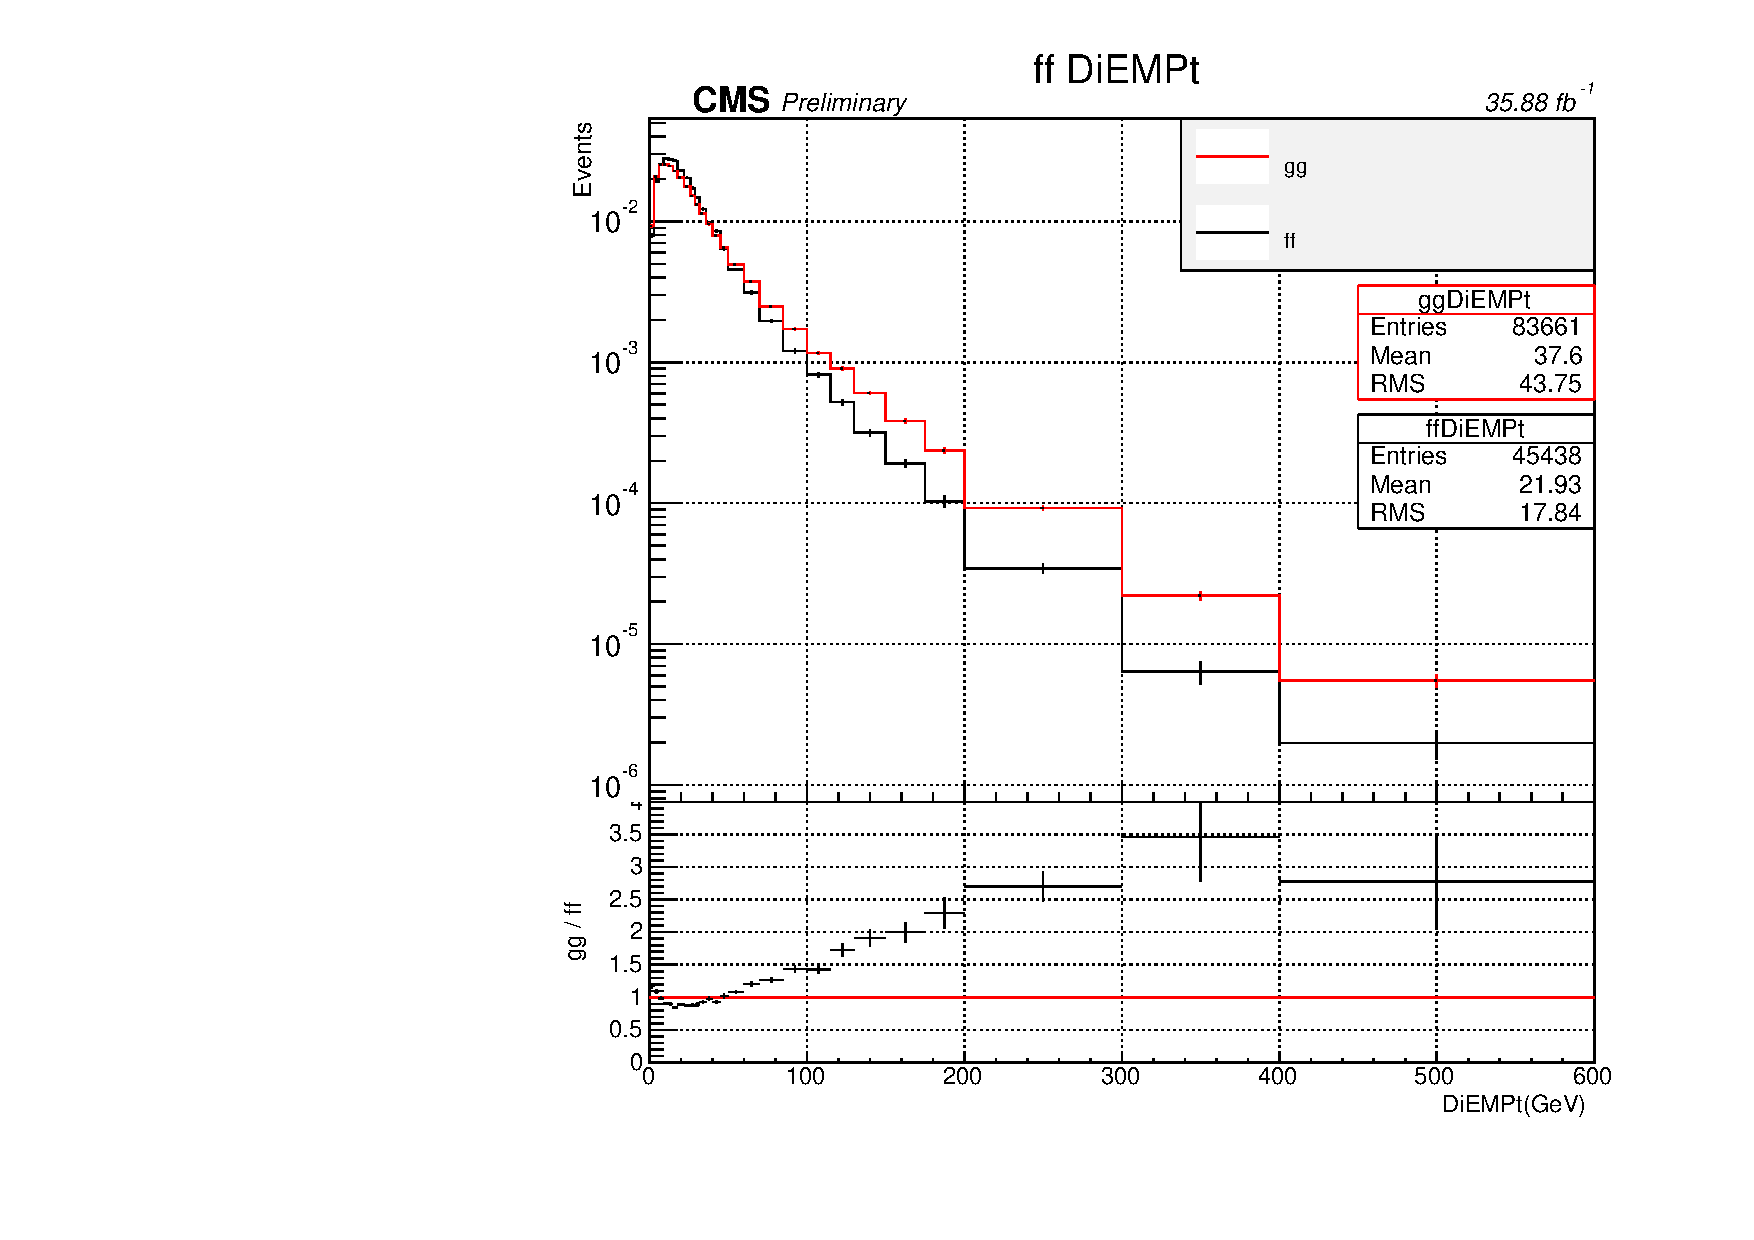
\includegraphics[width=0.9\textwidth]{Figures/DataAnalysis/ggffUnweighted.pdf}
\end{center}
\caption{\Diempt distributions of the $ff$ control sample (black) and the $\gamma\gamma$ candidate sample (red). The ratio plot on the bottom shows the $\gamma\gamma$/$ff$ ratios that are used to reweight the $ff$ \ETmiss distribution. }
\label{fig:ggffUnweighted}
\end{figure*}

\begin{figure*}[h]
\begin{center}
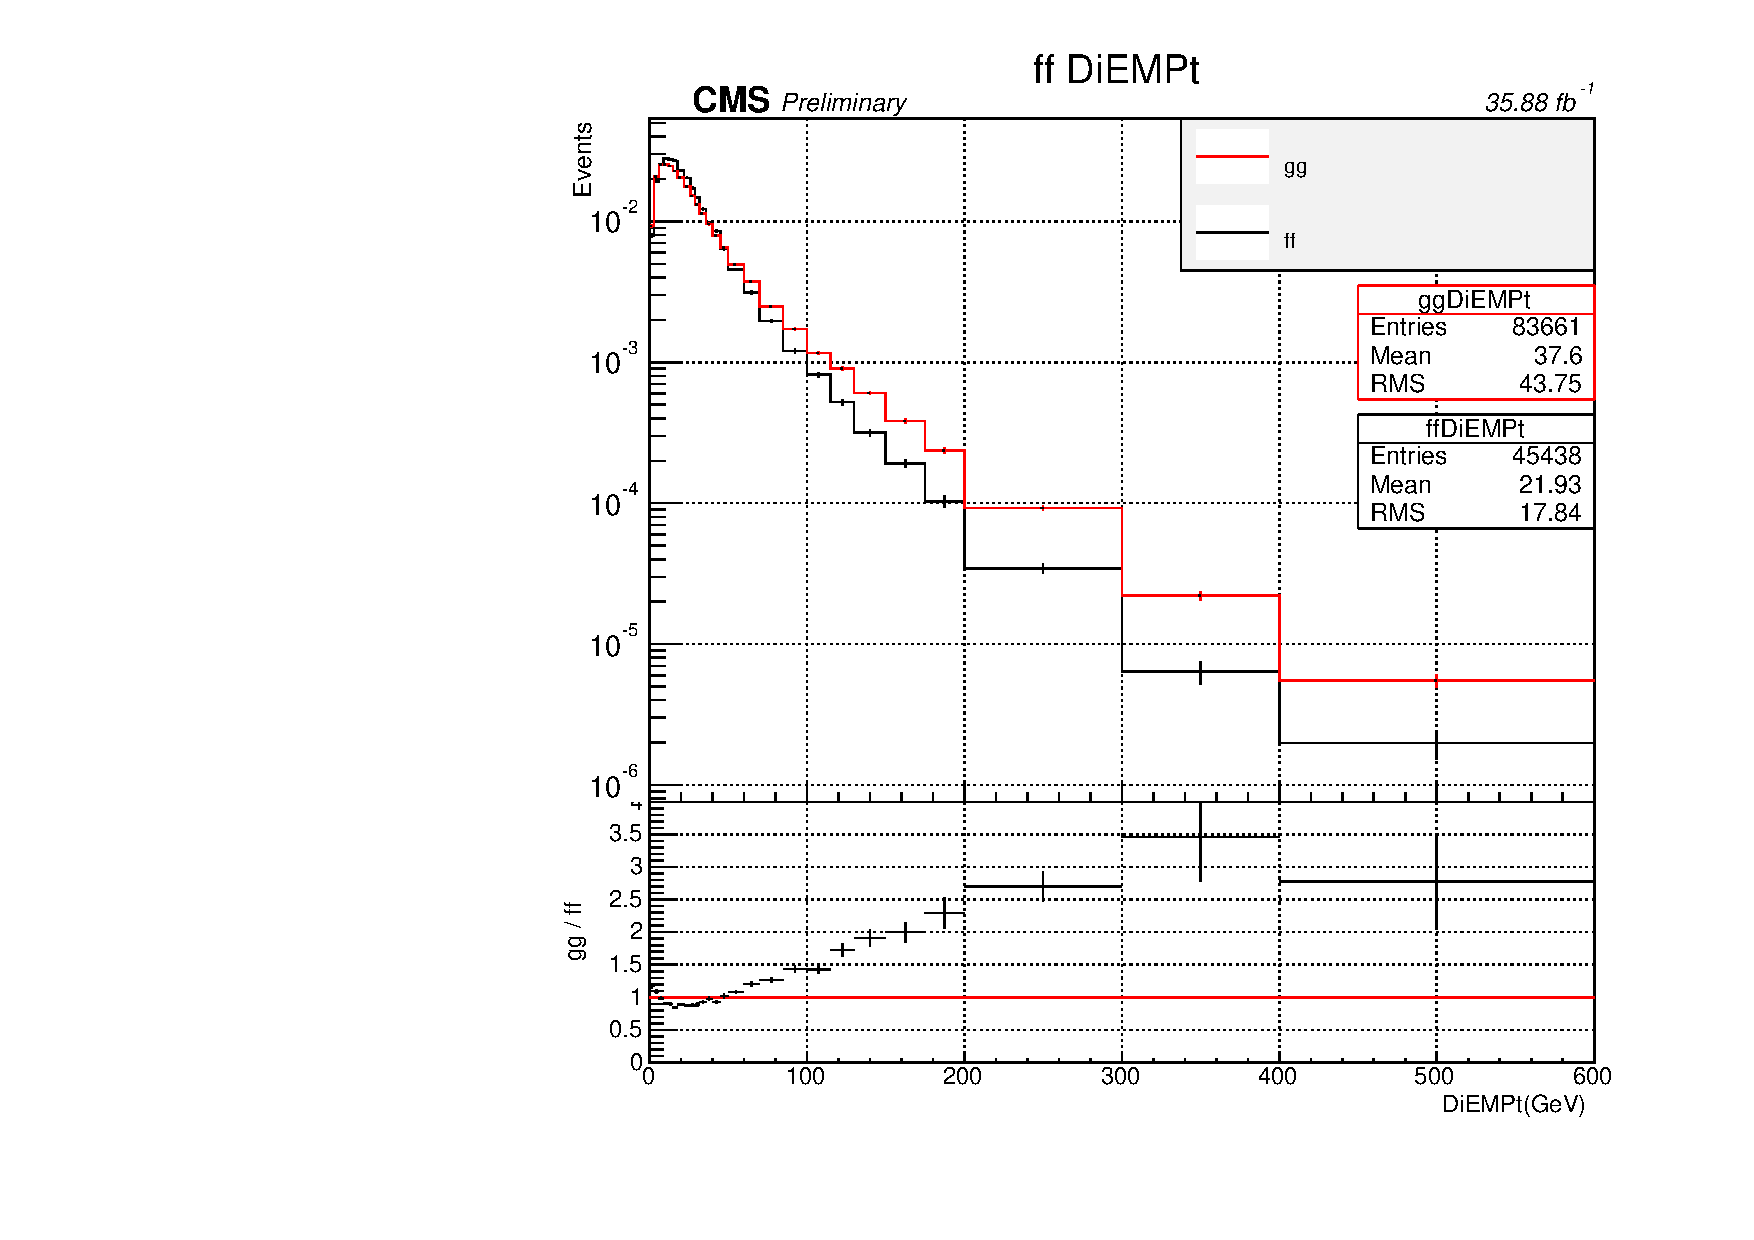
\includegraphics[width=0.9\textwidth]{Figures/DataAnalysis/compareUnweighted.pdf}
\end{center}
\caption{\Diempt distributions of the $ff$ control sample (black) and the $\gamma\gamma$ candidate sample (red). The ratio plot on the bottom shows the $\gamma\gamma$/$ff$ ratios that are used to reweight the $ff$ \ETmiss distribution. }
\label{fig:compareUnweighted}
\end{figure*}

\begin{figure*}[h]
\begin{center}
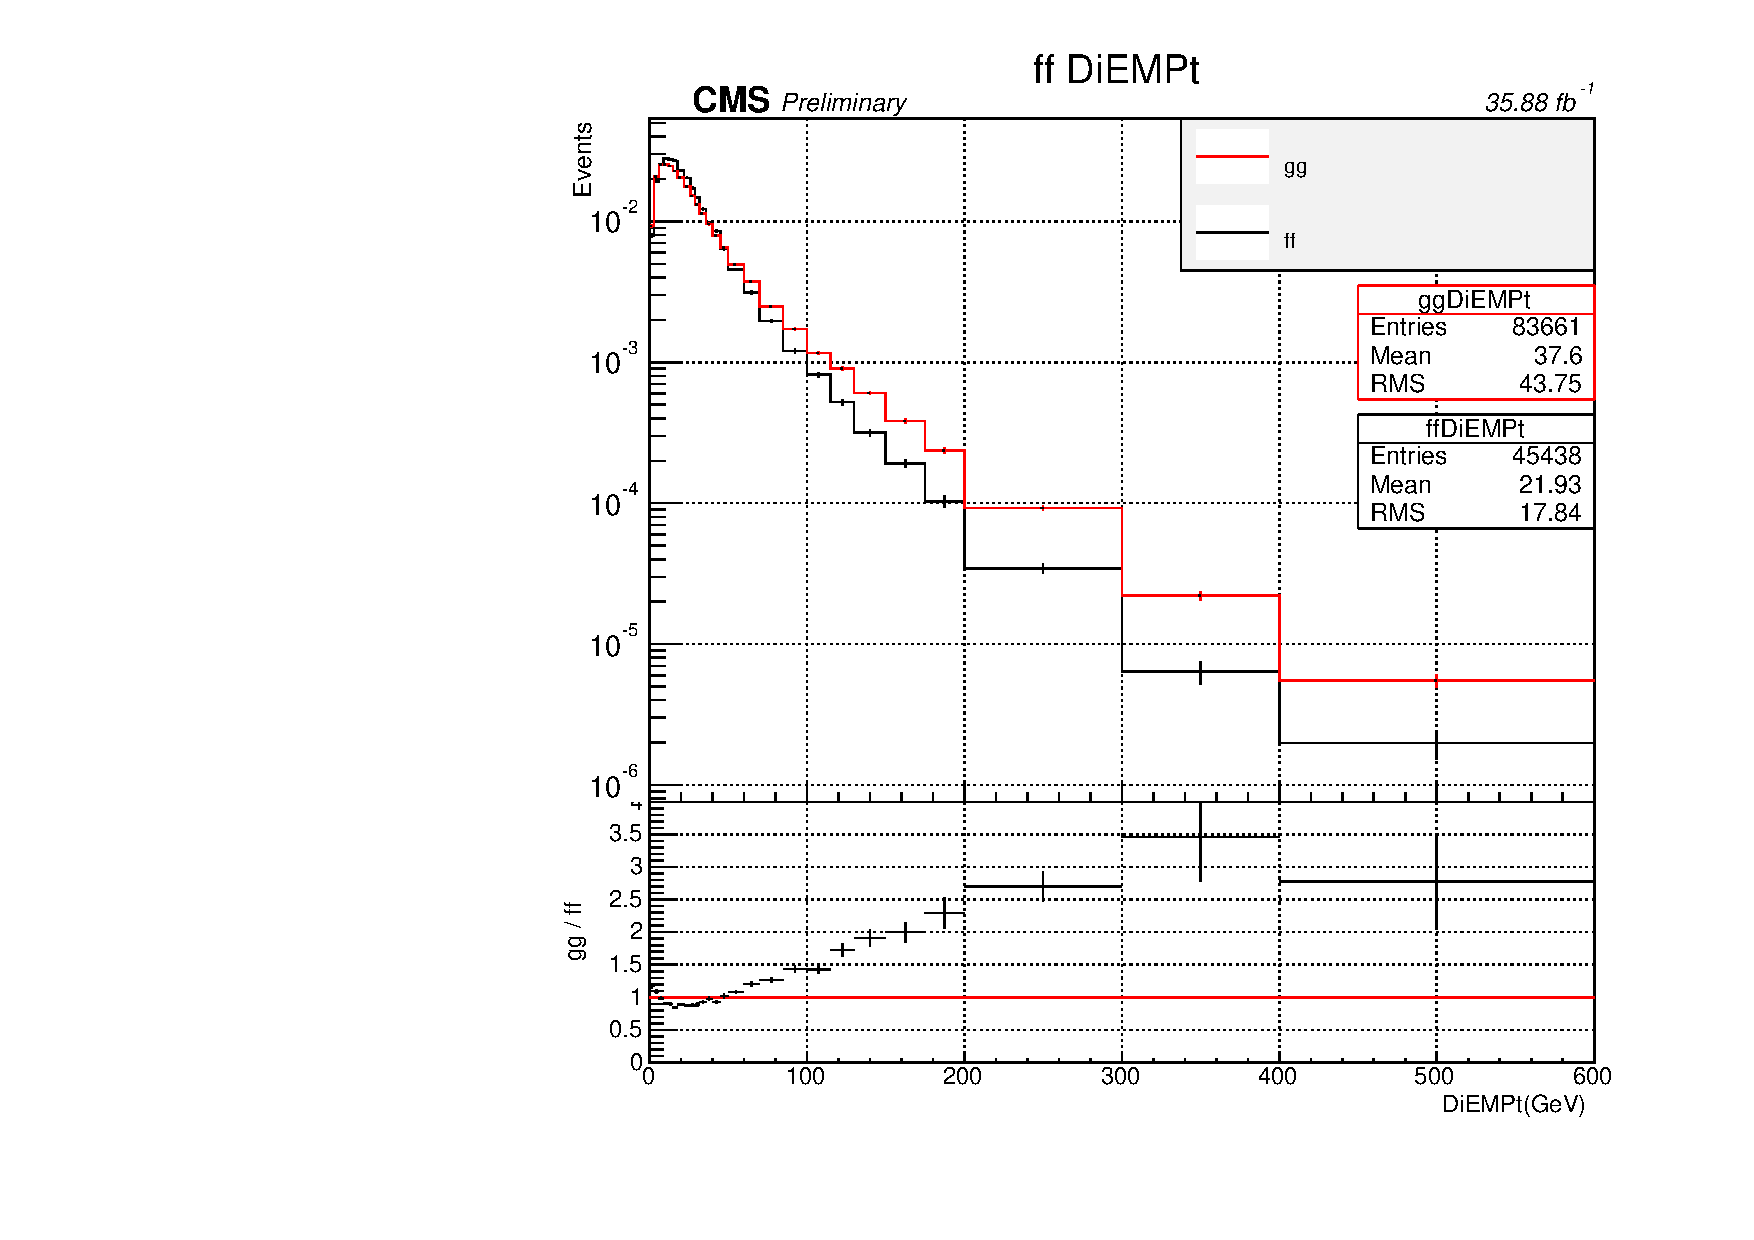
\includegraphics[width=0.9\textwidth]{Figures/DataAnalysis/ggffReweighted.pdf}
\end{center}
\caption{\Diempt distributions of the $ff$ control sample (black) and the $\gamma\gamma$ candidate sample (red). The ratio plot on the bottom shows the $\gamma\gamma$/$ff$ ratios that are used to reweight the $ff$ \ETmiss distribution. }
\label{fig:ggffReweighted}
\end{figure*}

%%%%%%Cross Check and Systematics%%%%%%

\subsection{Cross check on QCD background}
\label{sec:crossCheck}

In order to set a systematic uncertainty on the overall \ETmiss shape predicted using the \diempt reweighting method, we sought an alternate way to estimate the QCD background. This cross check relies on the assumption that the ratio of $\gamma\gamma$ events to $ff$ events should not depend sensitively on \ETmiss. If this assumption is true, then we should be able to extrapolate from the low-\ETmiss control region to the high-\ETmiss signal region.

\begin{figure*}[h]
\begin{center}
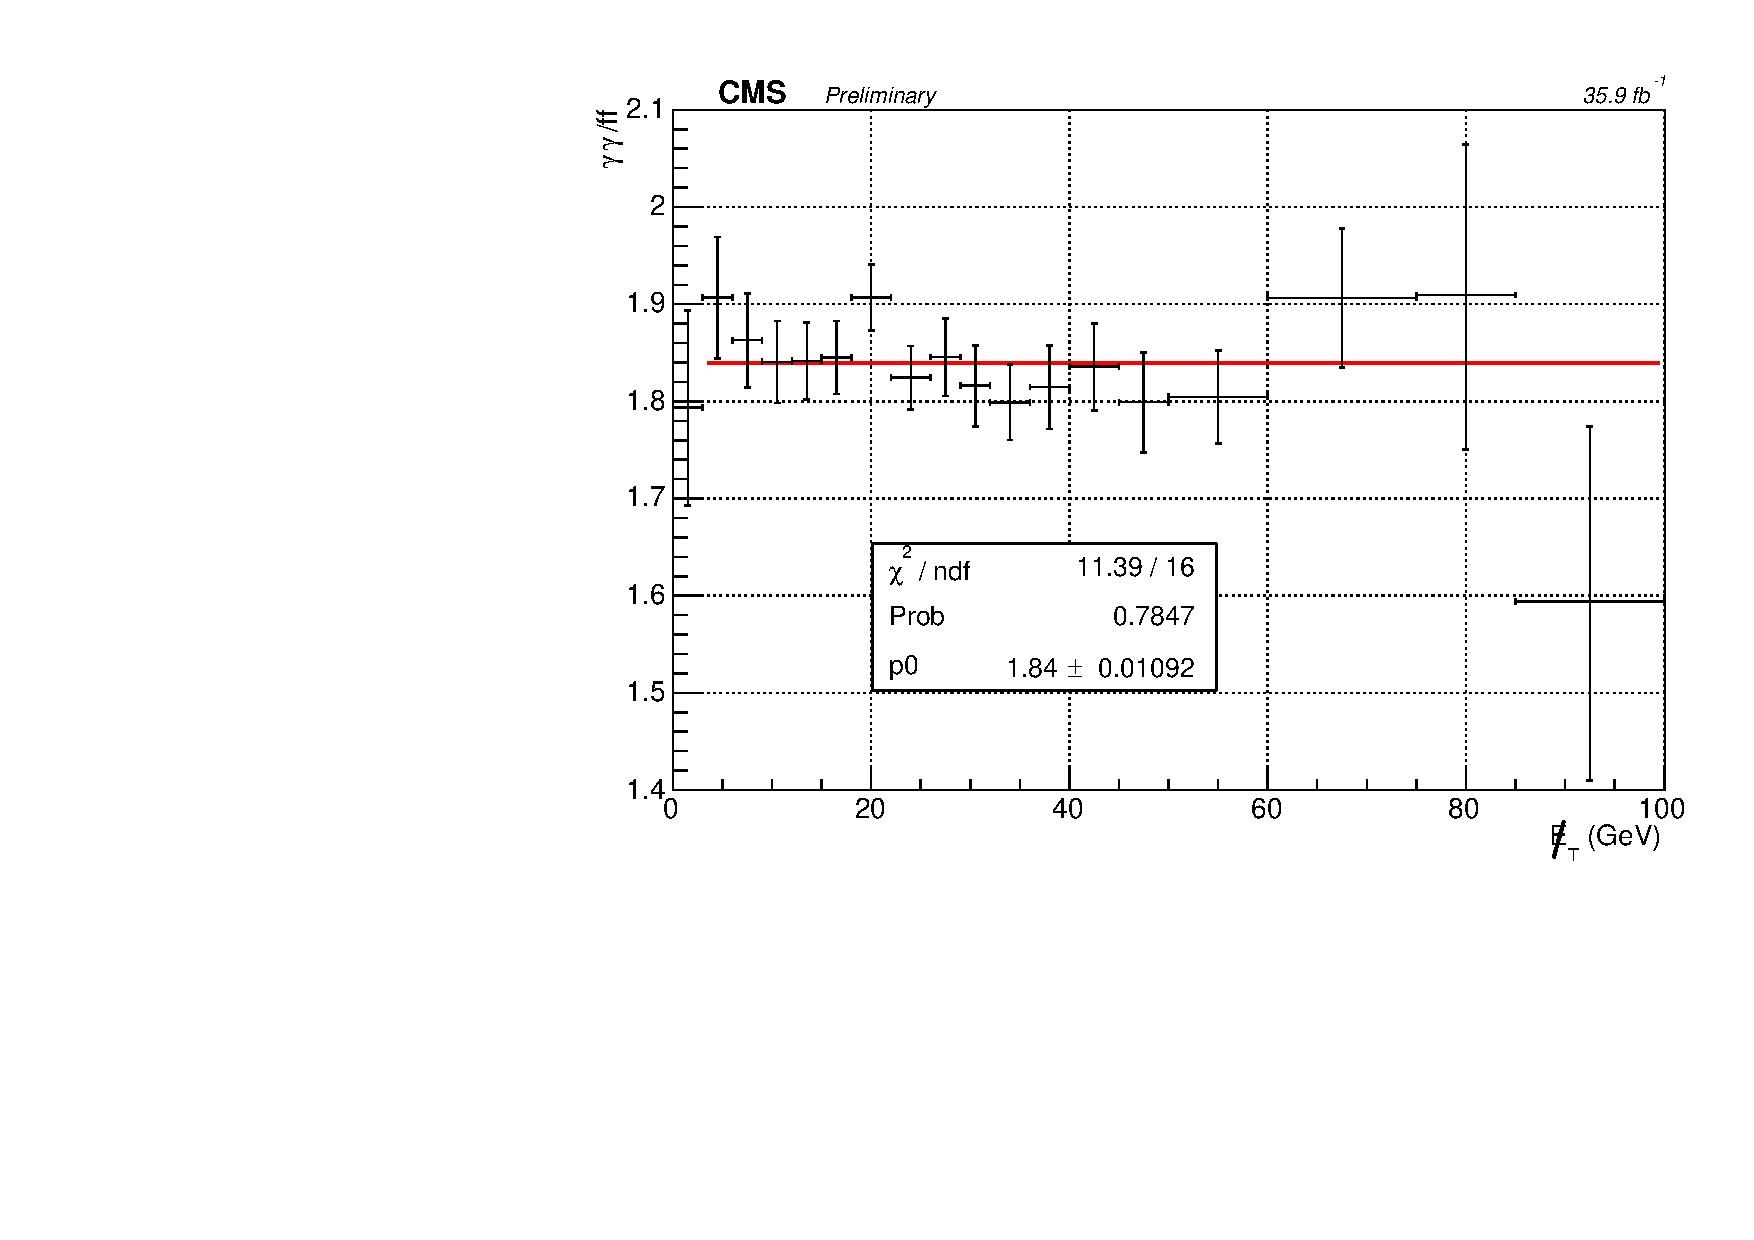
\includegraphics[width=0.9\textwidth]{Figures/DataAnalysis/crossCheckFit.pdf}
\end{center}
\caption{The ratio of $\gamma\gamma$ to $ff$ events for \ETmiss$ < 100$ GeV. 
The ratio has been fit to a constant function, which can then be used to 
extrapolate to the \ETmiss$ >100$ GeV signal region. 
This provides an alternative estimation method for the QCD background.}
\label{fig:crossCheck}
\end{figure*}

Figure~\ref{fig:crossCheck} shows the ratio of $\gamma\gamma$/$ff$ as a function of \ETmiss in the \ETmiss $<$ 100 GeV control region. The ratio has been fit to a constant function $f(\ETmiss)$. Using this function, the expected number of $\gamma\gamma$ events in bin $i$ of the signal region is given by the following equation:

\begin{equation}
N_{\gamma\gamma}^i = f(\ETmiss) \times N_{ff}^i 
\end{equation}

Table~\ref{tab:crossCheck} compares the expected QCD background contribution as predicted with the cross check method to that predicted with the \diempt reweighting method. For the cross check method, the uncertainty arising from the choice of fitting function is estimated by taking the difference between the results when fitting to a constant to the results when fitting to a linear function. In addition, the cross check uncertainties listed in Table~\ref{tab:crossCheck} include the statistical uncertainty from the limited control sample statistics and the $1~\sigma$ uncertainties from the fit. For the \diempt reweighting method, the uncertainties include the statistical uncertainty and the uncertainty from the \diempt reweighting procedure (this systematic is described in detail in Section~\ref{sec:QCDSysUncert}). 

\begin{table}[ht]
     \caption{COMPARISON BETWEEN REWEIGHTING METHOD AND RATIO METHOD FOR THE QCD BACKGROUND ESTIMATE}
     \centering
     {\renewcommand{\arraystretch}{1.2} %<- modify value to suit your needs                                                            
     \begin{tabular}{| c | c | c | c |}
     \hline
     \hline
    \ETmiss bin (Gev) & Reweighted ff estimate & Ratio method estimate \\
     \hline
    $100-115$ & ${69.23}^{+ 15.18}_{-12.68}$ & ${ 55.19}^{+ 12.03}_{-10.33}$ \\
    $115-130$ & ${30.89}^{+ 11.76}_{-8.82}$  & ${ 22.08}^{+ 8.39}_{-6.59}$ \\
    $130-150$ & ${25.98}^{+ 11.95}_{-8.61}$  & ${ 16.55}^{+ 7.56}_{-5.69}$ \\
    $150-185$ & ${20.49}^{+ 10.12}_{-7.11}$  & ${ 14.72}^{+ 7.26}_{-5.45}$ \\
    $185-250$ & ${8.74}^{+ 11.65}_{-5.89}$   & ${ 3.68}^{+ 4.85}_{-2.47}$ \\
    $> 250$     & ${5.13}^{+ 11.86}_{-4.43}$   & ${ 1.84}^{+ 4.23}_{-1.60}$ \\
     \hline
     \hline
     \end{tabular}
}
	\justify{Comparison of the background estimate using the di-EM \pt reweighting method and the $\gamma\gamma$/$ff$ ratio method. The uncertainties on the 
	 di-EM \pt reweighting method include the statistical uncertainties and the reweighting uncertainty. The uncertainties on the ratio method include the 
	 statistical uncertainties, the uncertainties in the fit parameter, and the uncertainty from the choice of fit function. }
     \label{tab:crossCheck}
\end{table}


The two methods give overlapping predictions
within uncertainty, and therefore this cross check serves to validate our di-EM \pt reweighting
background estimation method. The difference between the two methods
is taken as a systematic uncertainty on the overall \ETmiss shape.

%%%%%%%%%%%%%%%%%%%%%%%%%%%%%%%%%%%%%%%
%%%%%%%%EWK background %%%%%%%%%%%%%%%%%%%%%%
%%%%%%%%%%%%%%%%%%%%%%%%%%%%%%%%%%%%%%%

\section{Electroweak background}
\label{sec:EWK}

The subdominant background for this search is comprised of W$\gamma$ and W+jet events where W$\rightarrow e \nu$ and the electron is misidentified as a photon. This background is referred to as the electroweak (EWK) background. Unlike the QCD background, there is inherent \ETmiss in these events from the escaping neutrino. 

To estimate this background, we first calculate the rate at which electrons are misidentified as photons. This is done by comparing the invariant mass peak in a double electron sample ($ee$) with the invariant mass peak in a sample of events with one electron and one photon ($e\gamma$). The composition of the $e\gamma$ control sample is investigated in Section~\ref{sec:EWKMC} and the calculation of this ``fake rate" is described in detail in Section~\ref{sec:fakeRate}. To get the final expected contribution from the EWK background in our signal region, the fake rate is used to calculate a transfer factor (Section~\ref{sec:transfer}). By applying the transfer factor to an $e\gamma$ control sample, we are able to estimate how many of our candidate $\gamma\gamma$ events are actually events with one photon and one electron that has been misidentified as a photon (Section~\ref{sec:EWKresults}). 

%%%%%%%%%%%%%%%%%%%%%%%%%%%%%%%%%%%%%%%

\subsection{Composition of $e\gamma$ sample}
\label{sec:EWKMC}
The $e\gamma$ control sample is primarily made up of $\gamma~+$ jets or W$\gamma$ events. A data versus MC comparison of this control sample is shown in Figure~\ref{fig:dataMCEG}. The data distribution was fit using the simulated $\gamma~+$ jet and W$\gamma$ shapes as templates. From the fit, it was determined that 80\% of the $e\gamma$ events observed in data are from $\gamma~+$ jets  processes, and the remaining 20\% are W$\gamma$ events.  
In the \ETmiss$>100$~GeV signal region, however, W$\gamma$ events dominate.
For $100 < \ETmiss < 130$~GeV, 12.1\% of the MC prediction is made up of
$\gamma~+$ jet processes. For $\ETmiss >130$~GeV, 
$\gamma~+$ jet events contribute only 2.6\%.

\begin{figure*}[h!]
	\centering
	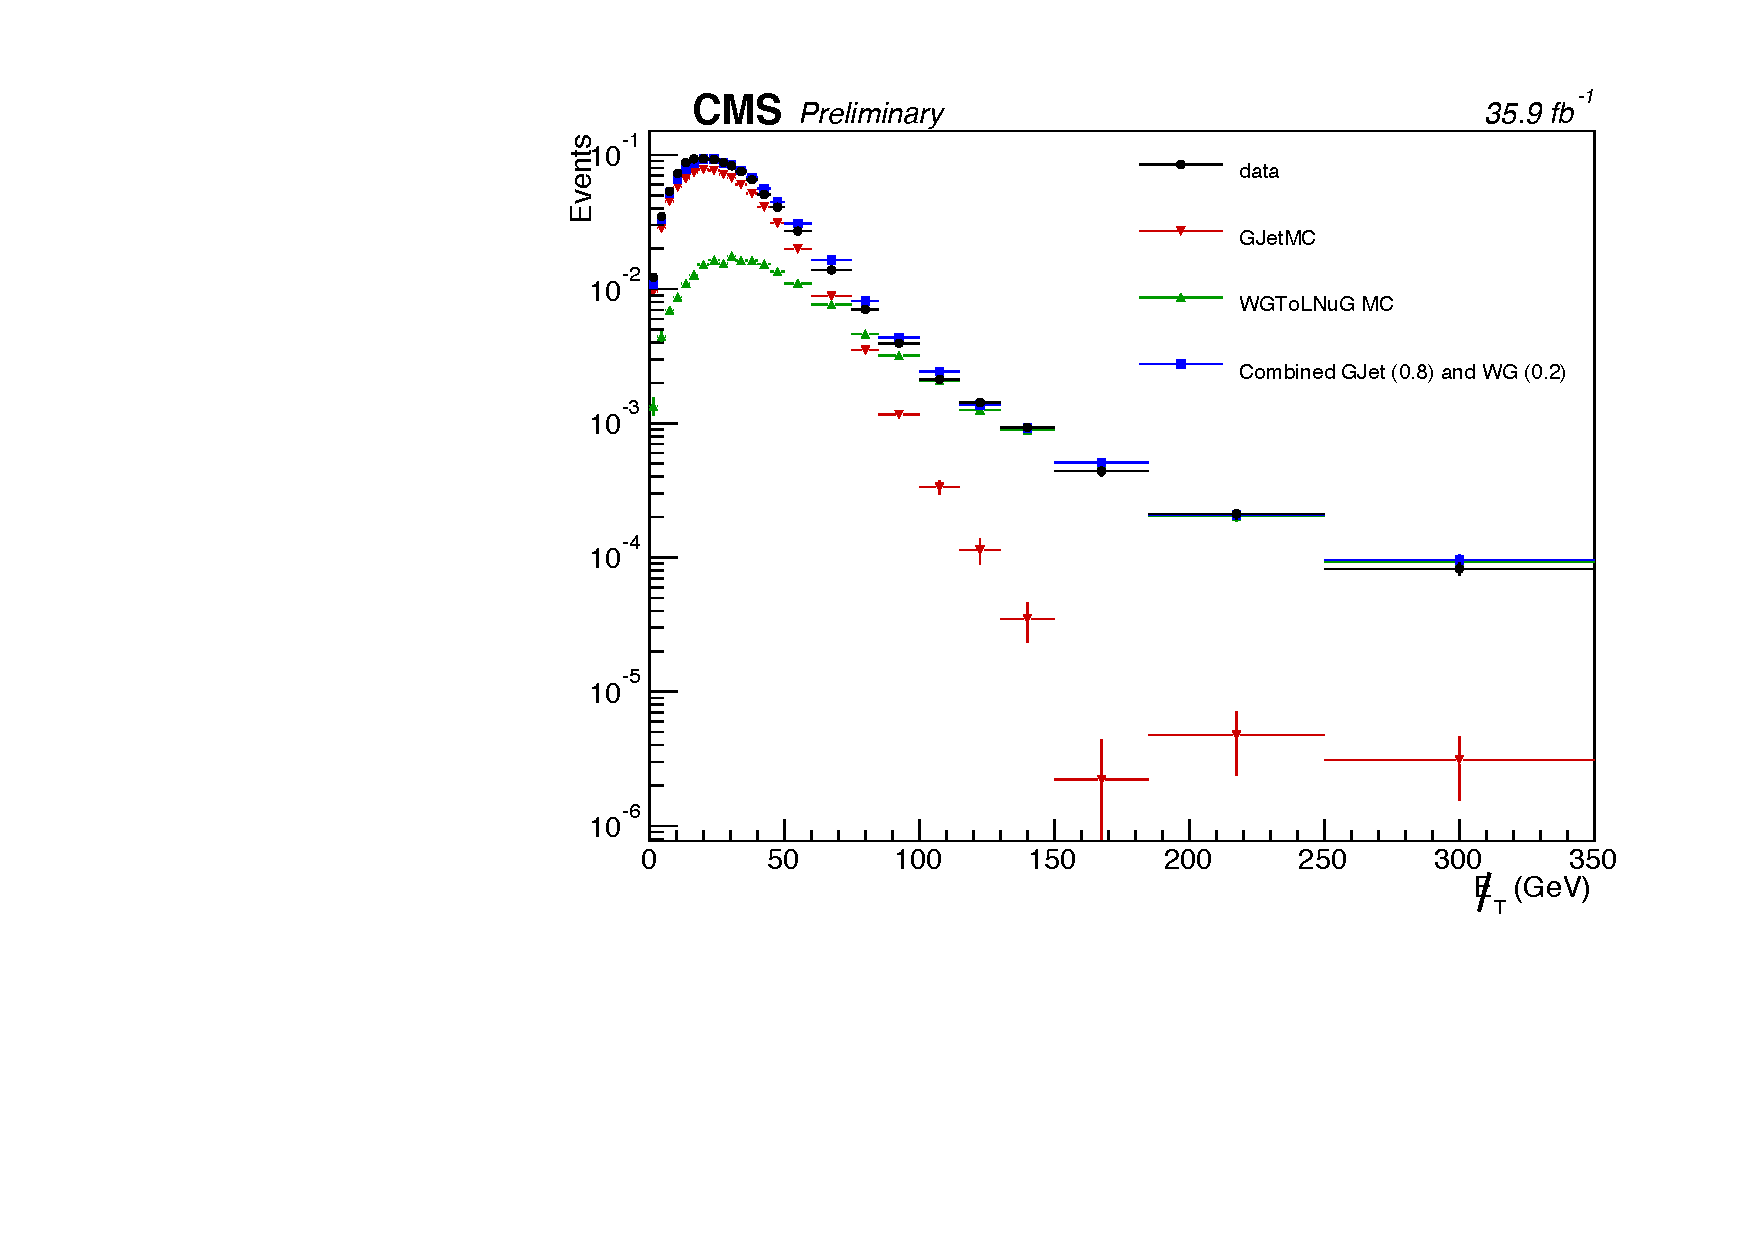
\includegraphics[width=0.8\textwidth]{Figures/DataAnalysis/dataMC_EG.pdf}
       \caption{Data versus MC comparison of the $e\gamma$ control sample \ETmiss distribution. To determine the relative contributions of the
       $\gamma~+$ jet and W$\gamma$ processes, the data distribution was fit using the $\gamma~+$ jet and W$\gamma$ shapes as templates. The data
       are shown in black, and the total MC prediction is shown in blue. The $\gamma~+$ jet MC (red) was scaled to 80\% of the observed events in data. and 
       the W$\gamma$ MC (green) was scaled to 20\% of the data distribution.
	}
   	\label{fig:dataMCEG}
\end{figure*}

%%%%%%%%%%%%%%%%%%%%%%%%%%%%%%%%%%%%%%%

\subsection{Fake rate calculation}
\label{sec:fakeRate}

A tag and probe method is used for the fake rate calculation. Events are selected using a single electron trigger. Electrons passing medium ID criteria and 
satisfying \pT $> 30$ GeV and $|\eta| < 2.1$ are used as tags. The tags are required to be matched to the object firing the single electron trigger within \dR$ < 0.2$. 
Probes are photon candidates with \pT $> 40$ GeV that pass all of the identification criteria described in Chapter~\ref{chap:EventSelect} except for the pixel seed veto. The tag and probe objects are required to be separated by \dR$ > 0.3$ and have an invariant mass between 40 and 140 GeV. If there are multiple tag and probe pairs in a single event, all possible combinations are considered. If the probe has a pixel seed, then it is labeled as an electron and falls into the $ee$ sample. If the probe does not have a pixel seed, however, then it is labeled as a photon and is included in the $e\gamma$ sample. 

Because processes other than $Z\rightarrow ee$ decays can be included in this sample, a fit is performed on each invariant mass distribution. The shape of the invariant mass peak in $Z\rightarrow ee$ MC is used as a signal template, and an electron + muon control region in data is used as the background template. After fitting the $ee$ and $e\gamma$ distributions in data, the integrals of the signal shapes between 80 and 100 GeV are referred to as $N_{ee}^Z$ and $N_{e\gamma}^Z$, respectively. 
Figure~\ref{fig:invMassShapes} shows the shapes of the data distributions as well as the background and signal templates with arbitrary normalization. The results after the fit are shown as well. 

\begin{figure*}[h]
\begin{center}
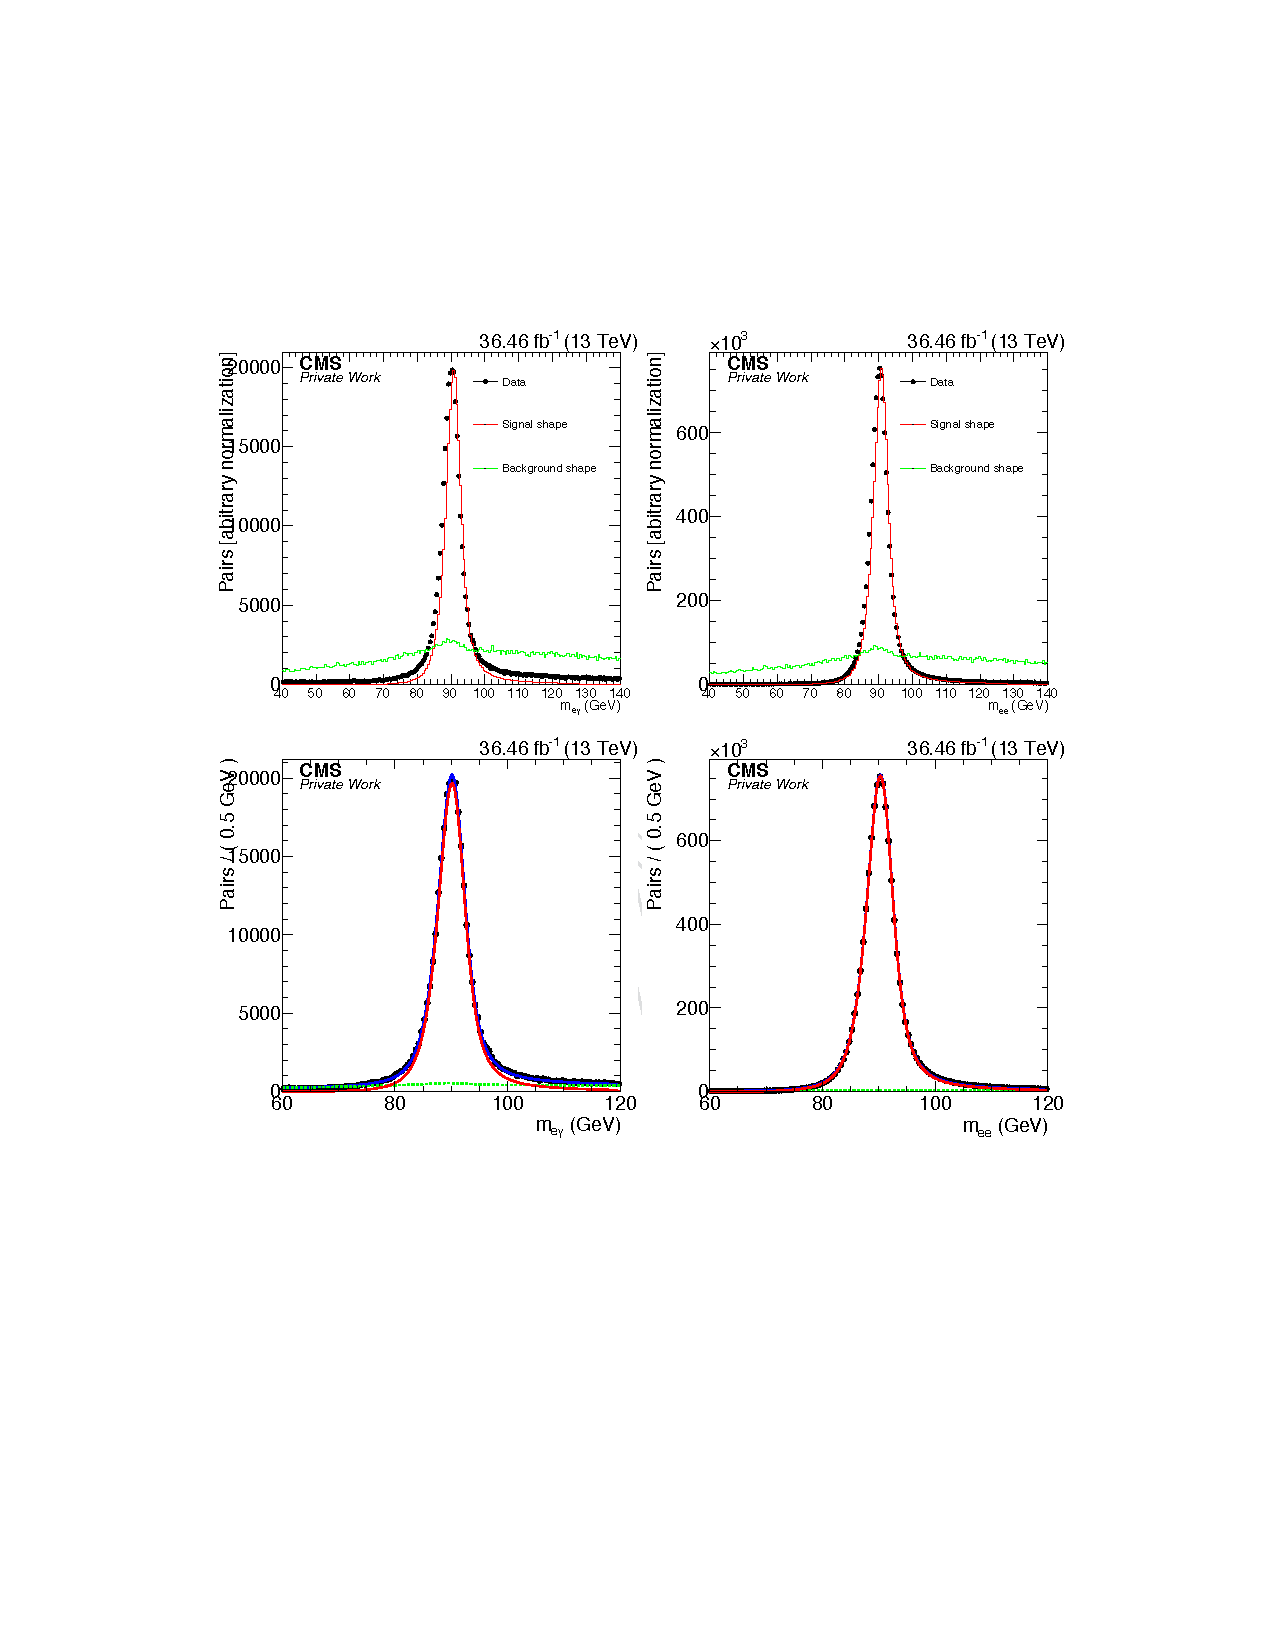
\includegraphics[width=\textwidth]{Figures/DataAnalysis/EWKInvMassShapes.pdf}
\end{center}
\caption{Invariant mass distributions for the $e\gamma$ (left) and $ee$ (right) samples. Each plot includes the data (black markers), 
the signal template (red), and the background template (green). The top plots demonstrate the shape of each distribution with arbitrary 
normalization, and the bottom plots show the distributions after the fits are performed.
}
\label{fig:invMassShapes}
\end{figure*}

The maximum of the background shape at 90 GeV arises from the \pT thresholds of the tag and probe objects. The \pT distributions tend to be sharply falling, so most probes have a \pT around 40 GeV and most tags have a \pT around 30 GeV. Changing the probe \pT threshold changes the position of the peak in the background template.

The ratio $R_{\gamma/e} = N_{e\gamma}^Z/N_{ee}^Z$ is calculated from the fits and found to be $R_{\gamma/e} = 2.63\%$ overall. The fits are performed in bins of different kinematic variables to investigate any potential dependencies of $R_{\gamma/e}$. These are shown in Figures~\ref{fig:fakeRateKin1} and \ref{fig:fakeRateKin2}. 

\begin{figure*}[h]
\begin{center}
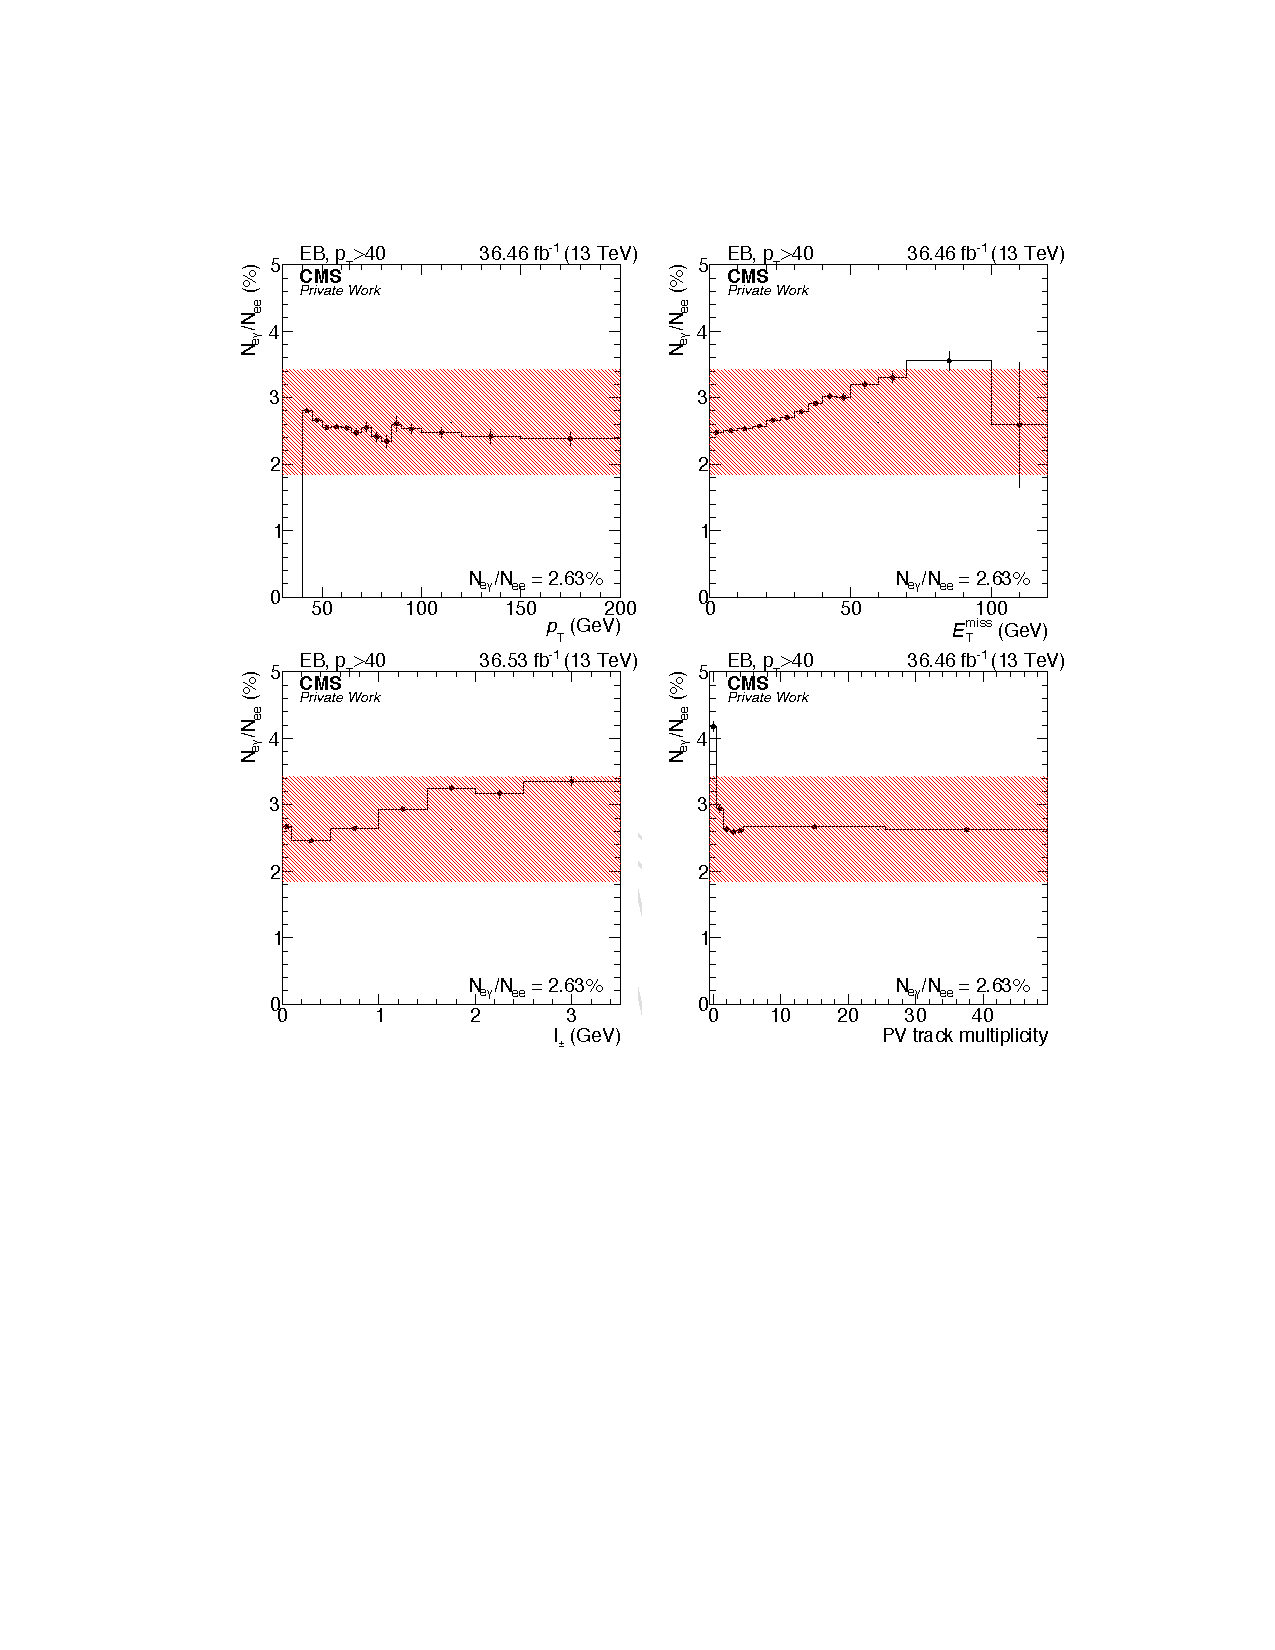
\includegraphics[width=\textwidth]{Figures/DataAnalysis/fakeKin1.pdf}
\end{center}
\caption{Value of $R_{\gamma/e}$ as a function of various kinematic variables for probes in the barrel: probe \pT, \ETmiss, isolation I$_{\pm}$, 
and track multiplicity of the primary vertex (PV). The red band corresponds to a 30\% uncertainty 
on $R_{\gamma/e}$.
}
\label{fig:fakeRateKin1}
\end{figure*}

\begin{figure*}[h]
\begin{center}
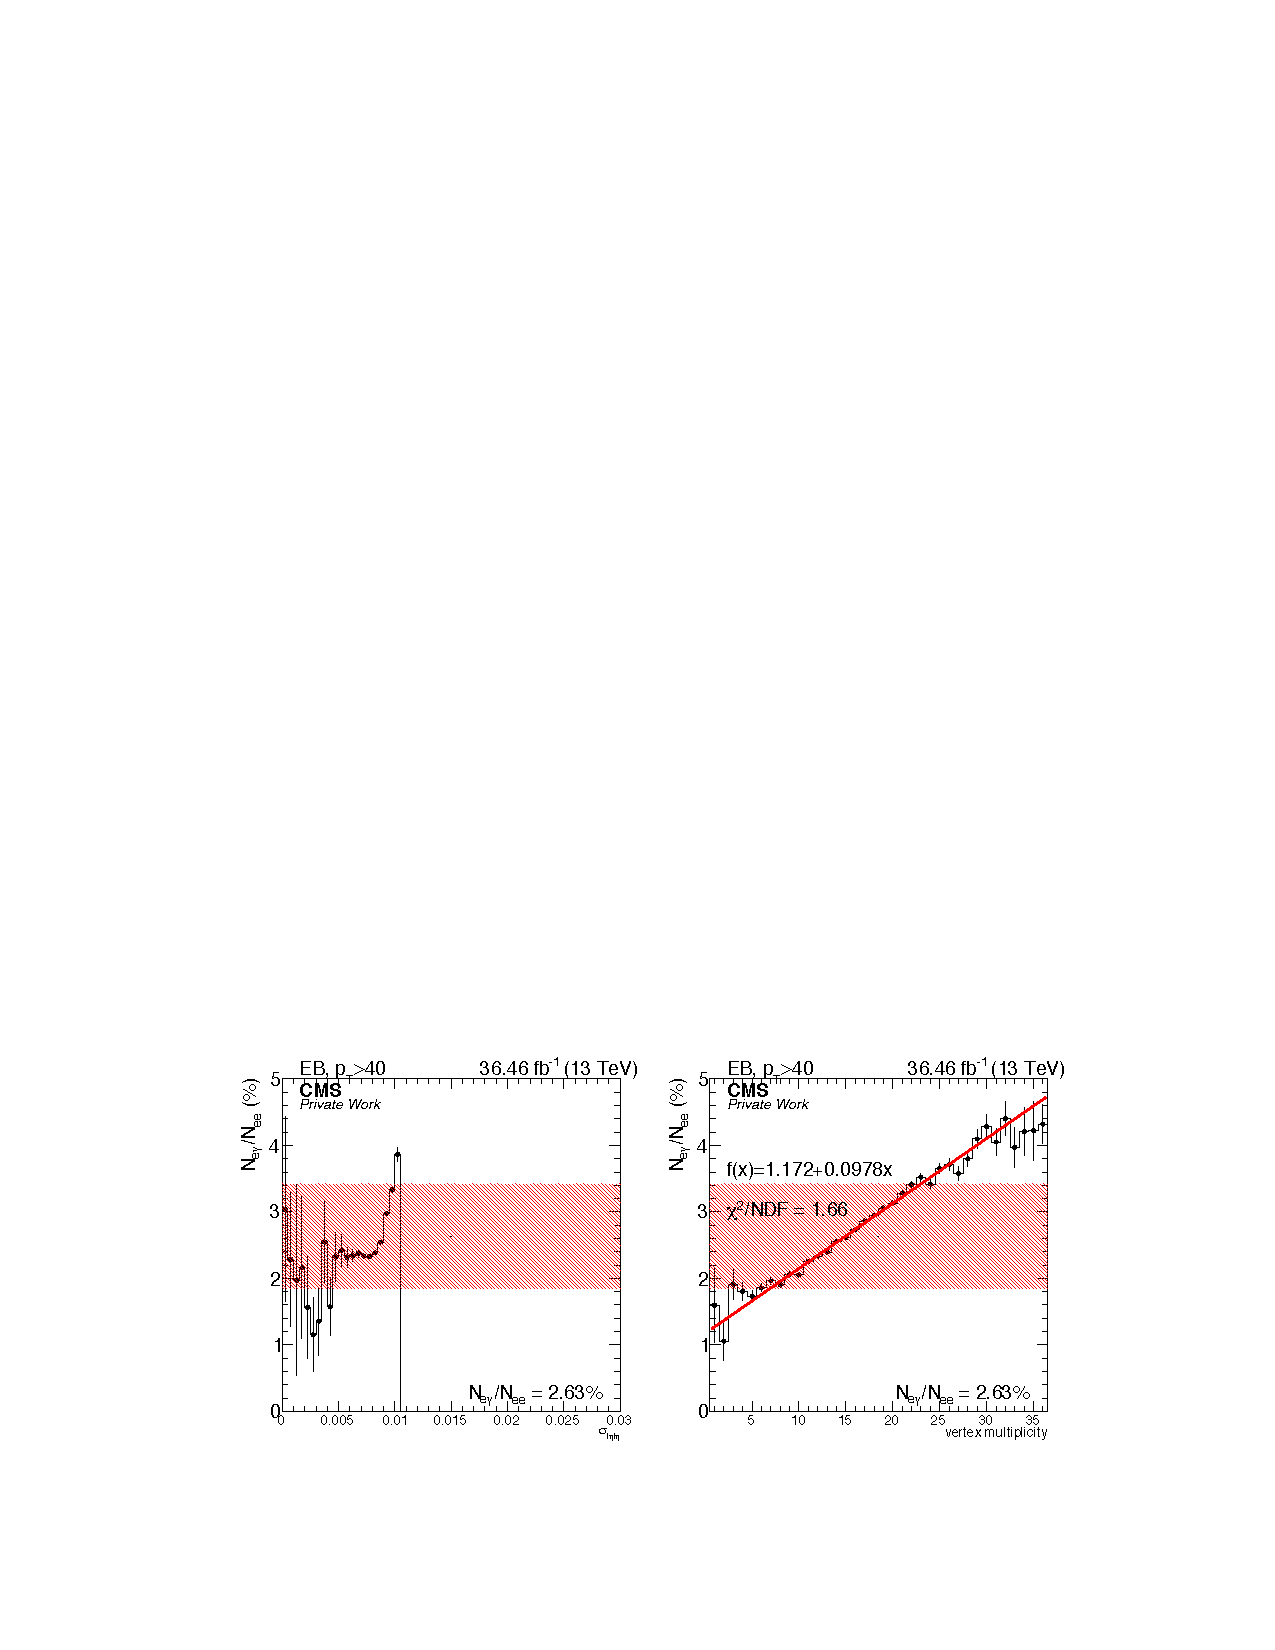
\includegraphics[width=\textwidth]{Figures/DataAnalysis/fakeKin3.pdf}
\includegraphics[width=\textwidth]{Figures/DataAnalysis/fakeKin2.pdf}
\end{center}
\caption{Value of $R_{\gamma/e}$ as a function of various kinematic variables for probes in the barrel: \sigmaietaieta of the probe, 
vertex multiplicity, jet multiplicity, and probe $|\eta|$. The red band corresponds to a 30\% uncertainty 
on $R_{\gamma/e}$.
}
\label{fig:fakeRateKin2}
\end{figure*}

A 30\% systematic uncertainty is assigned to the ratio $R_{\gamma/e}$ to cover the observed dependencies. 
This is shown in the red bands in Figures~\ref{fig:fakeRateKin1} and \ref{fig:fakeRateKin2}. The strongest dependency is with respect
to the vertex multiplicity. Recall that vertex multiplicity is a proxy for the number of pileup interactions in the event. For a similar analysis that 
used this fake rate XX cite Knut XX, $R_{\gamma/e}$ was parameterized as a function of the vertex multiplicity, but no significant difference was found between 
applying the linear fit shown in Figure~\ref{fig:fakeRateKin2} rather than the constant value of 2.63\%.

The distinctive features of $R_{\gamma/e}$ as a function of $|\eta|$ are due to detector effects. Similar features are seen in data quality monitoring plots showing the occupancy of the ECAL crystals as a function of $\eta$ and $\phi$. 

%%%%%%%%%%%%%%%%%%%%%%%%%%%%%%%%%%%%%%%

\subsection{Calculating EWK estimate}
\label{sec:transfer}
The number of observed $Z\rightarrow ee$ events in the $e\gamma$ and $ee$ mass spectra can be expressed as a function of $f_{e\rightarrow\gamma}$, the rate at which electrons are misidentified as photons:
\begin{equation}
\begin{aligned}
\label{equ:fake}
N_{e\gamma}^Z &= f_{e\rightarrow\gamma}(1- f_{e\rightarrow\gamma})N_{Z}'\\
N_{ee}^Z &= (1-f_{e\rightarrow\gamma})^2N_{Z}'
\end{aligned}
\end{equation}
where $N_{Z}'$ is the actual number of $Z\rightarrow ee$ events. 

%Solving for $f_{e\rightarrow\gamma}$, we get
%\begin{equation}
 %f_{e\rightarrow\gamma} = N_{e\gamma}/(2N_{ee}+N_{e\gamma})
%\end{equation}

If we then consider a generic sample of $N_{e\gamma}'$ events with a real photon and a real electron, 
the number of events $N_{e\gamma}$ that will actually get reconstructed as having one photon and one electron is given by:
\begin{equation}
N_{e\gamma}=(1-f_{e\rightarrow\gamma})N_{e\gamma}'
\end{equation}

The background $N_{\gamma\gamma}$, the fraction of $N_{e\gamma}'$ that ends up in the candidate
$\gamma\gamma$ sample, can be written as:
\begin{equation}
N_{\gamma\gamma} = f_{e\rightarrow\gamma} N_{e\gamma}' = N_{e\gamma}\frac{f_{e\rightarrow\gamma}}{1-f_{e\rightarrow\gamma}}
\end{equation}

By looking at Equation~\ref{equ:fake}, it can be seen that this last factor is precisely the ratio $R_{\gamma/e} = N_{e\gamma}^Z/N_{ee}^Z = 2.63\%$ that was discussed above. Thus, the EWK background prediction is simply given by $R_{\gamma/e}$ times the number of observed $e\gamma$ events. 

%%%%%%%%%%%%%%%%%%%%%%%%%%%%%%%%%%%%%%%

\subsection{EWK results}
\label{sec:EWKresults}

Table XX shows the final EWK estimate in the six signal region bins. There are two sources of uncertainty on the EWK estimate: the statistical uncertainty from the limited number of $e\gamma$ events observed in data, and the 30\% systematic uncertainty from the calculation of the fake rate. Both of these are included in the uncertainties listed in Table XX.


%%%%%%%%%%%%%%%%%%%%%%%%%%%%%%%%%%%%%%%
%%%%%%%%ZGG background %%%%%%%%%%%%%%%%%%%%%%
%%%%%%%%%%%%%%%%%%%%%%%%%%%%%%%%%%%%%%%

\section{Irreducible background}
\label{sec:Zgg}

In addition to the QCD and EWK backgrounds, there is a small irreducible background from $Z\gamma\gamma\rightarrow\nu\nu\gamma\gamma$ events. Because there is inherent \ETmiss from this process, it is not included in the QCD background, and because it has two true photons, it is not included in the EWK background either. We model this background using MC simulation and assign a 50\% uncertainty to the estimate to cover any potential mismodeling. The predicted background from $Z\gamma\gamma$ events is shown in Table~\ref{tab:ZGG}.

XX Table XX 

%\subsection{Cross checking normalization}
%\label{sec:ZggNorm}
%To cross check the $Z\gamma\gamma$ normalization obtained from data, we compare the observed number of $Z\gamma\gamma\rightarrow ee \gamma\gamma$ events seen in data to that predicted via MC. These processes are different only in the decay mode of the $Z$ boson, and therefore should give an accurate indication of how well the process is simulated in MC. The results are shown in Table XX. 

%%%%%%%%%%%%%%%%%%%%%%%%%%%%%%%%%%%%%%%
%%%%%%%%Uncertainties %%%%%%%%%%%%%%%%%%%%%%
%%%%%%%%%%%%%%%%%%%%%%%%%%%%%%%%%%%%%%%

\section{Systematic uncertainties}
The systematic uncertainties fall into two main categories: 
those associated with one of the background estimates,
and other uncertainties used in the limit-setting procedure.

\subsection{Uncertainties on background estimates}
\label{sec:QCDSys}
The largest uncertainties on the background estimate come from the QCD prediction method.
The uncertainties on the QCD estimate are summarized for each \ETmiss bin in the signal region in
Table~\ref{tab:QCDSysUncert}. All uncertainties are expressed as numbers of events.

One of the uncertainties on the QCD estimate comes from the \diempt reweighting procedure. Recall that to
correct for differences in hadronic activity in the events, the \ETmiss distribution of the $ff$ sample 
is reweighted by \diempt, so that its \diempt spectrum matches that of the double photon
candidate sample. To propagate the uncertainty from the \diempt reweighting, we generated
one thousand different \diempt ratios. In each case, the value of the ratio in each bin is obtained by varying the
nominal \diempt ratio using a Gaussian distribution with $\sigma$ equal to the statistical uncertainty of that bin. 
We then reweight the \ETmiss distributions of the $ff$ control sample with the 1000
generated \diempt ratios. Final uncertainties are then determined from the fluctuations in each
\ETmiss bin by finding the range that includes 68\% of the new \ETmiss values. 

 Another systematic uncertainty on the QCD background estimation comes from the 
 uncertainty in the overall \ETmiss shape. To estimate this uncertainty, we use the ratio method 
 described in Section~\ref{sec:crossCheck} as a cross-check. 
 By fitting the ratio of $\gamma\gamma$ to $ff$ at low \ETmiss to a constant, 
 the expected number of $\gamma\gamma$ events at high \ETmiss can be extrapolated from the observed 
 number of $ff$ events. This procedure gives us a second estimates for the QCD background in each
bin of \ETmiss. The difference between the two estimates is taken as a symmetric
systematic uncertainty and is shown in the second-to-last column
of Table~\ref{tab:QCDSysUncert}.

As described above, there are two uncertainties on the EWK background: 
the statistical uncertainty from the limited statistics in the control region and 
the 30\% uncertainty on the $e\rightarrow\gamma$ fake rate. 
For the $Z\gamma\gamma$ background, the only uncertainty considered is 
a 50\% uncertainty to cover any potential mismodeling of the \ETmiss shape or 
uncertainty on the $Z\gamma\gamma\rightarrow\nu\nu\gamma\gamma$ cross section. 

\subsection{Other sources of systematic uncertainties}
\label{sec:otherSys}

In addition to the systematic uncertainties arising from the background estimation techniques
described above, there are other systematic uncertainties that affect the
final analysis sensitivity. These uncertainties are summarized in Table~\ref{tab:SysUncert}. 
Ranges of uncertainty arise when there are different values for the uncertainty
for different signal points.
 
The first is the uncertainty in the Parton Distribution Functions (PDF?s) and the variation of 
cross section ratios (K factors) between leading order PDF?s
and next-to-leading order PDF?s. The PDF uncertainties are taken from the NNPDF30 variations XX cite XX .

Other uncertainties on the signal include finite MC statistics and the photon data/MC scale
factor described in Section~\ref{sec:phoSF}. There is also a 2.5\% uncertainty on the integrated
luminosity of the data sample \cite{lumiPAS}. 

Finally, an additional source of uncertainty comes from propagating the jet energy scale uncertainty described in Section~\ref{sec:JEC} to the \ETmiss. 
The expected signal yields are re-calculated using the 1 $\sigma$ fluctuations of \ETmiss if the jet energy scale is varied by its uncertainty. The difference between the yields with and without the jet energy scale changes is taken as a systematic uncertainty. 

%The nominal \ETmiss value is calculated using jets with only the Type-I corrections applied. 





  \chapter{Results and Interpretations}
\label{chap:Results}

\section{Prediction versus observation}
\label{sec:fullCount}
After deriving estimates for all Standard Model backgrounds, we compare the number of 
observed events with the expected number of background events. 
The \ETmiss distributions for the full background prediction and the unblinded data are
shown in Figure~\ref{fig:FinalPlot}. Three benchmark signal models are also shown, 
corresponding to the T5gg simplified model 
(described in detail in Section~\ref{sec:SimplifiedModels}) with gluino mass equal to 1700 GeV.

Table~\ref{tab:ExpObs} shows the expected and observed numbers of events for each bin in the signal region.
Within the uncertainties, no excess is observed with respect to the Standard Model prediction.


\begin{table}[ht]
    \caption{EXPECTED AND OBSERVED EVENTS IN THE SIGNAL REGION}
    \centering
    \begin{tabular}{ |c|c|c|c|c|c|}
        \hline
        $\ETmiss$ (GeV) & Exp. QCD & Exp. EWK &  Z$\gamma\gamma$ events  &Total exp. & Observed \\ [0.5ex]
        \hline
        $100 - 115$ & ${69.23}^{+20.67}_{-18.91}$ & 8.17 $\pm$2.5  & 1.30$\pm$0.65 & ${ 78.69 }^{+ 22.58 }_{- 20.98 }$ & 65  \\
        $115 - 130$ & ${30.89}^{+14.69}_{-12.46}$ & 5.50 $\pm$1.70 & 1.14$\pm$0.57 & ${ 37.53 }^{+ 16.05 }_{- 14.04 }$ & 27 \\
        $130 - 150$ & ${25.98}^{+15.21}_{-12.76}$ & 4.78 $\pm$1.48 & 1.12$\pm$0.56 & ${ 31.88 }^{+ 16.44 }_{- 14.20 }$ & 17 \\
        $150 - 185$ & ${20.49}^{+11.65}_{-9.16} $ & 3.95 $\pm$1.24 & 1.32$\pm$0.66 & ${ 25.76 }^{+ 12.80 }_{- 10.59 }$ & 13 \\
        $185 -  250$& ${8.74} ^{+12.70}_{-7.765}$ & 3.52 $\pm$1.11 & 1.28$\pm$0.64 & ${ 13.55 }^{+ 13.05 }_{- 8.31  }$ & 8  \\
        $\geq 250$  & ${5.13} ^{+12.31}_{-5.514}$ & 2.11 $\pm$0.69 & 1.14$\pm$0.57 & ${ 8.38  }^{+ 12.48 }_{- 5.88  }$ & 10 \\
        \hline
    \end{tabular}
    \label{tab:ExpObs}
\end{table}

\begin{figure*}[h]
\begin{center}
\includegraphics[width=0.9\textwidth]{Figures/Results/finalPlot.pdf}
\end{center}
\caption{\ETmiss distributions for the full background estimation and the observed data. The black points represent the observed \ETmiss distribution. 
The QCD background is shown in red, the EWK background
is shown in blue, and the $Z\gamma\gamma$ background is shown in green. 
The combined uncertainty on the background estimation is shown in yellow.}
\label{fig:FinalPlot}
\end{figure*}

%%%%%%%%%%%%%%%%%%%%%%%%%%%%%%%%%%%%%%%

\section{Simplified Models}
\label{sec:SimplifiedModels}

Two simplified models are used in the interpretation of the results. The T5gg simplified model assumes gluino (\gluino) pair production and the T6gg model assumes squark (\squark) pair production. Example decay chains for both models are shown in Figure~\ref{fig:gluinoSquarkDecay}.

\begin{figure*}[htbp]
    \centering
    \includegraphics[width=0.45\textwidth]{Figures/Results/gluinoDecay.pdf}
    \includegraphics[width=0.45\textwidth]{Figures/Results/squarkDecay.pdf}
    \caption{Diagrams showing the production of signal events in the collision
        of two protons with four momenta ${P}_{1}$ and ${P}_{2}$. In gluino
        \gluino~pair production in the T5gg simplified model (left), the gluino
       decays to an antiquark \antiquark, quark q, and neutralino \neutralino. In
        squark \squark~pair production in the T6gg simplified model (right), the
        squark decays to a quark and a neutralino. In both cases, the
        neutralino subsequently decays to a photon $\gamma$~and a gravitino \gravitino.
        In the diagram on the right, we do not distinguish between squarks and
        antisquarks.}
    \label{fig:gluinoSquarkDecay}
\end{figure*}

In both models, the lightest supersymmetric particle (LSP) is the gravitino, \gravitino, which is taken to be nearly massless. The next-to-lightest supersymmetric particle (NLSP) is the neutralino, \neutralino. The models assume 100\% branching fraction for 
$\neutralino\rightarrow\gravitino\gamma$ and 
$\gluino\rightarrow \mathrm{q} \antiquark \neutralino$ and 
$\squark\rightarrow \mathrm{q} \neutralino$.

In order to study the expected SUSY signal distributions, two
signal Monte Carlo scans were produced.
The T5Wg scan was produced in bins of gluino mass and neutralino mass,
and the T6Wg scan was produced in bins of squark mass and neutralino mass.
The leading-order event generator \textsc{MadGraph}5\_a\MCATNLO~\cite{Alwall:2014hca}
is used to simulate the signal samples, which
were generated with either two gluinos or two squarks and up to two additional
partons in the matrix element calculation. The parton showering, hadronization,
multiple-parton interactions, and the underlying event were described by the
\PYTHIA 8~\cite{Sjostrand:2007gs} program with the CUETP8M1 generator tune.
The detector response is simulated using
CMS fast simulation~\cite{Abdullin:2011zz}.

A total of 40,000 events were produced for
each bin, except for bins with gluino or squark masses above 2.0 TeV, where only
20,000 events were produced per bin.
For gluino masses from 1,400 to 2,500 GeV, events were generated
in bins of 50 GeV.  In the T6Wg scan, the squark masses ranged from
1,400 GeV to 2,050 GeV in bins of 50 GeV.
The neutralino masses ranged from 10 GeV up to the mass
of the gluino or squark and were binned in
100 GeV segments. Finer binning was used in the compressed region where
$M_{\neutralino}$ is within 300 GeV of $M_{\gluino}$ or $M_{\squark}$,
and in the region with low $M_{\neutralino}$.
These mass ranges were selected to overlap and
expand upon the mass ranges excluded by previous
searches~\cite{ATLAS:2016aa,CMS:2016_anal}.

The parton distribution
functions are obtained from NNPDF3.0~\cite{Ball:2014uwa}
The cross sections are calculated at NLO+NLL accuracy
~\cite{Kulesza:2009kq, Beenakker:2009ha},
with all the unconsidered sparticles assumed to be heavy and decoupled.
The uncertainties on the cross sections are calculated as
described in Ref. ~\cite{Borschensky:2014cia}.


%%%%%%%%%%%%%%%%%%%%%%%%%%%%%%%%%%%%%%%

\section{Signal acceptance and efficiency}

\section{Limits}

  \chapter{CONCLUSIONS}
\label{chap:Conclusions}

In this dissertation, a search for gauge-mediated supersymmetry breaking (GMSB) in events with two photons and missing transverse momentum was described. The analysis was performed with 35.9 \fbinv of data taken with the CMS detector in 2016. Fully data-driven background estimations were developed for the two primary backgrounds. For the QCD background, the background prediction was taken from a double fake control sample that had been reweighted by the $\gamma\gamma/ff$ \diempt distribution to correct for differences in hadronic activity. For the EWK background, we first calculated the rate at which photons were misidentified as photons by looking at the invariant mass spectrum in an $ee$ sample and an $e\gamma$ sample. This rate was then applied to an $e\gamma$ control sample satisfying the same criteria as the candidate $\gamma\gamma$ sample. Additionally, there is a small background from $Z\gamma\gamma\rightarrow\nu\nu\gamma\gamma$ events that was modeled in simulation. 

No evidence for GMSB was observed, and limits were placed on the masses of supersymmetric particles. Results were interpreted in the context of two simplified models, one assuming squark pair production and the other assuming gluino pair production. Gluino masses below 1.90 TeV and squark masses below 1.62 TeV are excluded at a 95\% confidence level.
  
  
 % Begin each chapter with \chapter{TITLE}. Chapter titles must be in all caps
 % and ensuring that they are is your responsibility.

\appendix

 % If you have appendices, add them here.
 % Begin each one with \chapter{TITLE} as before- the \appendix command takes
 % care of renaming chapter headings and creates a new page in the Table of
 % Contents for them.
 % \include{appendix-one}

\backmatter              % Place for bibliography and index


\bibliographystyle{nddiss2e}
 \bibliography{References}           % input the bib-database file name


\end{document}

%%
\endinput
%%
%% End of file `template.tex'.
